\begin{frame}[plain]
  \titlepage
  \note{[00:00--00:30] Introduce yourself as Morgan Hough, Executive Director of NeuroTechX. Thank the organizers. This talk is about NeuroTechX: what it is, what we do, how that work contributes to the community, and what it can mean for people building neurotech companies. The Tokyo meeting is the audience context.}
\end{frame}

% Career history supplied directly by Morgan Hough, September 5, 2026.
\section{My background}
\NTXDivider{About Me}
\begin{frame}{From Simple Systems Neurobiology\newline to HD-EEG \& Neuroimaging}
  \begin{columns}[c,onlytextwidth]
    \column{.61\textwidth}
      \fontsize{9.5}{11}\selectfont
      \textbf{A dual academic background}\par
      Biochemistry and molecular biology, alongside experimental psychology.\par\smallskip
      \textbf{Crustacean Behavioral Neurobiology Research Group}\par
      Started a student lab; built our own equipment to study operant conditioning in green crabs.\par\smallskip
      \textbf{After college: Karl Pribram}\par
      Worked on a novel high-density EEG system.\par\smallskip
      \textbf{Electrical Geodesics, Inc.}\par
      Worked under Don Tucker; later became software engineering manager.\par
    \column{.35\textwidth}
      \centering
      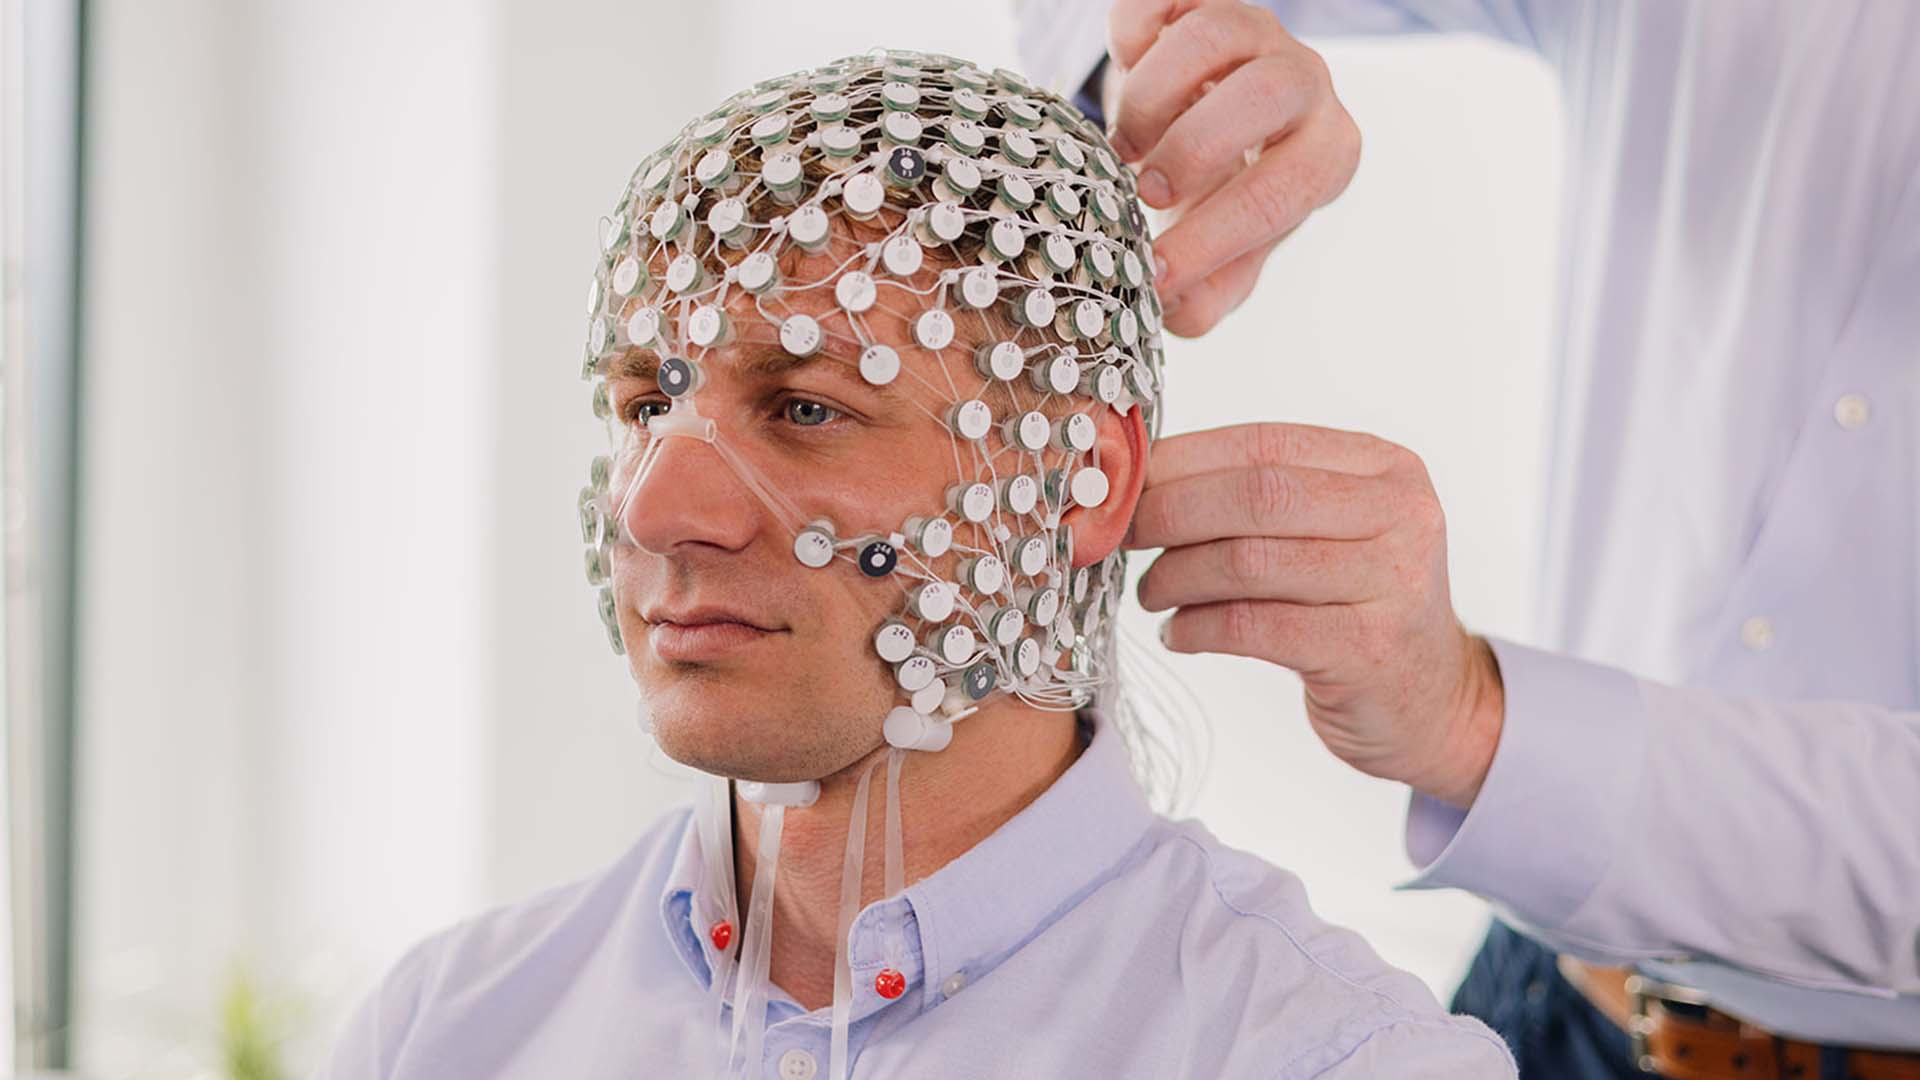
\includegraphics[width=\linewidth,height=20mm,keepaspectratio]{assets/history/egi-hd-eeg-sensor-net.jpg}
      \par{\tiny HD-EEG Geodesic Sensor Net\par}\smallskip
      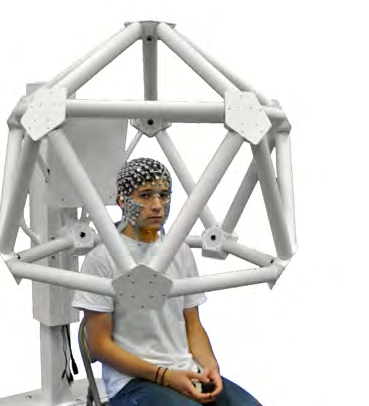
\includegraphics[width=\linewidth,height=22mm,keepaspectratio]{assets/history/egi-geodesic-camera-dome.png}
      \par{\tiny Geodesic Photogrammetry System\par}
  \end{columns}
  \smallskip{\tiny\color{NTXMuted}Equipment illustrations: \href{https://www.magstim.com/ges-500/}{Magstim EGI}; \href{https://www.egi.com/research-division/electrical-source-imaging/photogrammetry-sensor-digitization}{EGI sensor-digitization brochure}\par}
  \note{The right-hand images are official equipment illustrations, not Morgan or archival photos from his employment. The sensor-net photo comes from Magstim's GES 500 page; the camera dome was extracted from EGI's 2016 Sensor Digitization brochure. The Geodesic Photogrammetry System photographs electrode locations; it is distinct from the EEG sensor net. No claim is made that these particular product generations were the systems Morgan developed.}
  \note{[00:30--01:30] My academic background was dual: biochemistry and molecular biology, and experimental psychology. As a student I started the Crustacean Behavioral Neurobiology Research Group. We built our own equipment for studying operant conditioning in green crabs. This is an early example of the hands-on, collaborative approach that connects to the community-building story. After college I began working for Karl Pribram on a novel high-density EEG system. I was then hired by Electrical Geodesics, Inc., where I worked under Don Tucker and later became software engineering manager. The sequence and biographical details are supplied directly by Morgan; no degree titles, institutions, dates, or experimental results have been inferred.}
\end{frame}

\begin{frame}{UCSF and Oxford: neuroimaging methods}
  \begin{columns}[c,onlytextwidth]
    \column{.52\textwidth}
      \small
      \textbf{Dynamic Neuroimaging Lab, UCSF}\par
      Lab manager with Greg Simpson.\newline HD-EEG, MEG, and fMRI.\par\medskip
      \textbf{FMRIB, University of Oxford}\par
      Methods with Steve Smith and Mark Jenkinson in the Analysis Group.\par\medskip
      \textbf{Academic focus}\par
      Psychiatric applications of neuroimaging.\par\medskip
      \textbf{Physics-based head models}\par
      EEG, EIT, TES, TMS, and TFUS.\par
    \column{.44\textwidth}
      \centering
      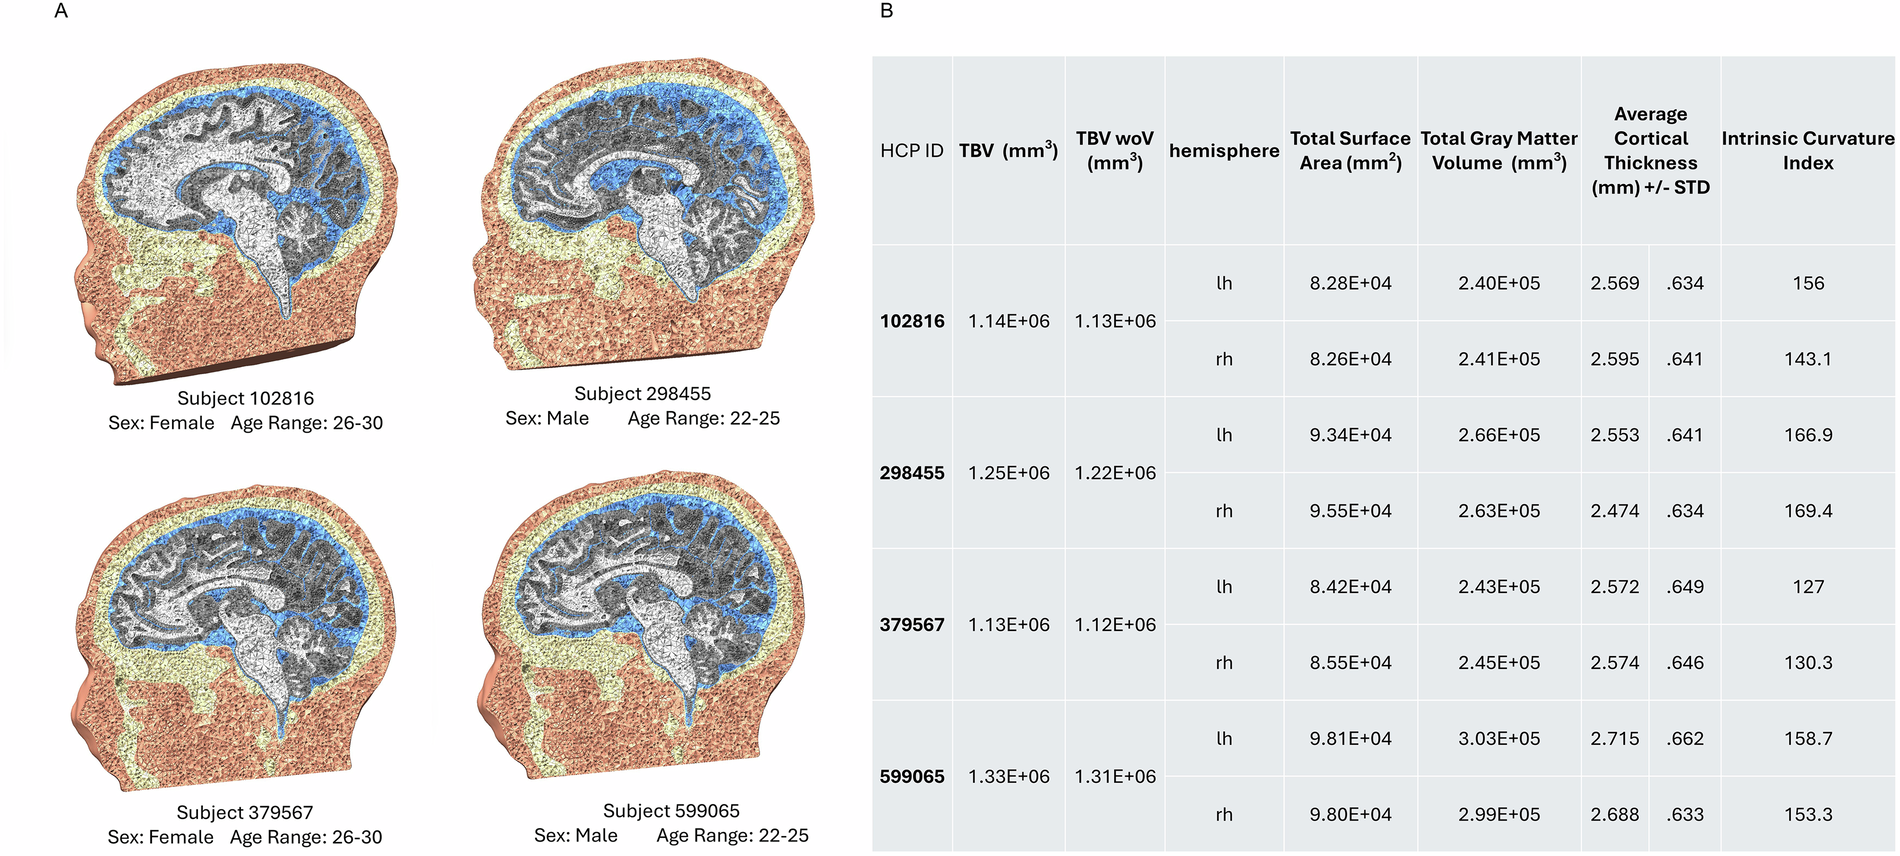
\includegraphics[trim=0bp 0bp 1040bp 0bp,clip,width=\linewidth,height=46mm,keepaspectratio]{assets/history/fem-berger-2025-fig2.png}
      \par\smallskip{\scriptsize MRI-derived finite-element head models\newline Skin, skull, CSF, eyes, gray and white matter\par}
  \end{columns}
  \smallskip{\tiny\color{NTXMuted}Image: \href{https://doi.org/10.1038/s41597-025-04886-0}{Berger et al., Scientific Data 12, 516 (2025), Fig.\ 2A}; cropped; \href{https://creativecommons.org/licenses/by/4.0/}{CC BY 4.0}\par}
  \note{Illustrative published finite-element head models, not Morgan's own results or Fijee output. Taylor A. Berger, Miles Wischnewski, Alexander Opitz, and Ivan Alekseichuk (2025), Human head models and populational framework for simulating brain stimulations, Scientific Data 12, 516, doi:10.1038/s41597-025-04886-0. Figure 2A shows four example subjects with six tissue types; subjects are not shown to scale. The slide crops out panel B's morphometric table without altering the models. Reused under CC BY 4.0.}
  \note{[01:30--02:30] At UCSF I was lab manager for the Dynamic Neuroimaging Lab under Greg Simpson, working with HD-EEG, MEG, and fMRI. At FMRIB, University of Oxford, I worked on methods development with Steve Smith and Mark Jenkinson in the Analysis Group. My academic work is primarily focused on psychiatric applications of neuroimaging. My technical expertise includes physics-based head models for EEG, EIT, TES, TMS, and TFUS. These descriptions are supplied directly by Morgan; they describe research focus and expertise, not claims of clinical efficacy or additional qualifications.}
\end{frame}

\begin{frame}{San Francisco: SKERI and Neuroscape}
  \begin{columns}[c,onlytextwidth]
    \column{.45\textwidth}
      \textbf{Smith Kettlewell Eye Research Institute}\par
      With Alex Wade\par\bigskip
      \textbf{Neuroscape at UCSF}\par
      With Adam Gazzaley
    \column{.51\textwidth}
      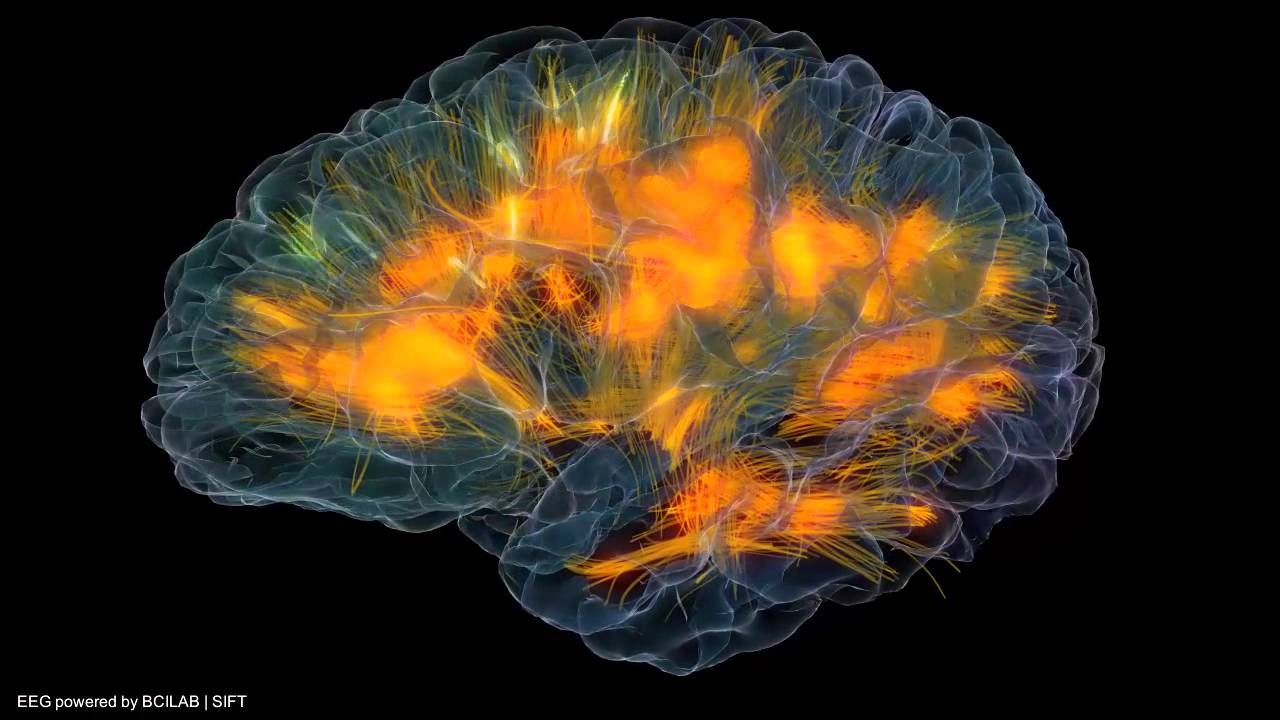
\includegraphics[width=\linewidth,height=43mm,keepaspectratio]{assets/history/neuroscape-glassbrain-video.jpg}
      \par\smallskip{\scriptsize Glass Brain --- MRI, diffusion imaging, and HD-EEG\newline Image: Neuroscape, UCSF\par}
  \end{columns}
  \smallskip{\tiny\color{NTXMuted}\href{https://neuroscape.ucsf.edu/technology/interventions-and-diagnostics/}{Neuroscape: Glass Brain}; \href{https://www.youtube.com/watch?v=dAIQeTeMJ-I}{official flythrough video}\par}
  \note{[02:30--03:00] After Oxford I returned to San Francisco: Smith Kettlewell Eye Research Institute with Alex Wade, then Neuroscape at UCSF with Adam Gazzaley. Glass Brain illustrates the Neuroscape setting: MRI and diffusion imaging provide anatomical context for HD-EEG activity visualization. This is the thumbnail of the official flythrough linked by Neuroscape, not a direct photograph of neural activity. Image credit: Neuroscape, UCSF. Their terms allow attributed non-commercial use but not commercial distribution or use as a presentation's primary feature. This supporting biography image is not the presentation's cover or central theme.}
\end{frame}

\begin{frame}{Back in San Francisco}
  \begin{columns}[c,onlytextwidth]
    \column{.55\textwidth}
      \small
      \textbf{Biopunk Lab}\par
      Founding Member --- synthetic neurobiology\par\smallskip
      \textbf{Neurotech@Frontier Tower}\par
      Lead\par\smallskip
      \textbf{Other Minds Lab}\par
      Co-founder\par\smallskip
      \textbf{Orthogonal Research \& DevoWorm Group}\par
      Lab Member\par\smallskip
      \textbf{NeuroTechX}\par
      Executive Director
    \column{.41\textwidth}
      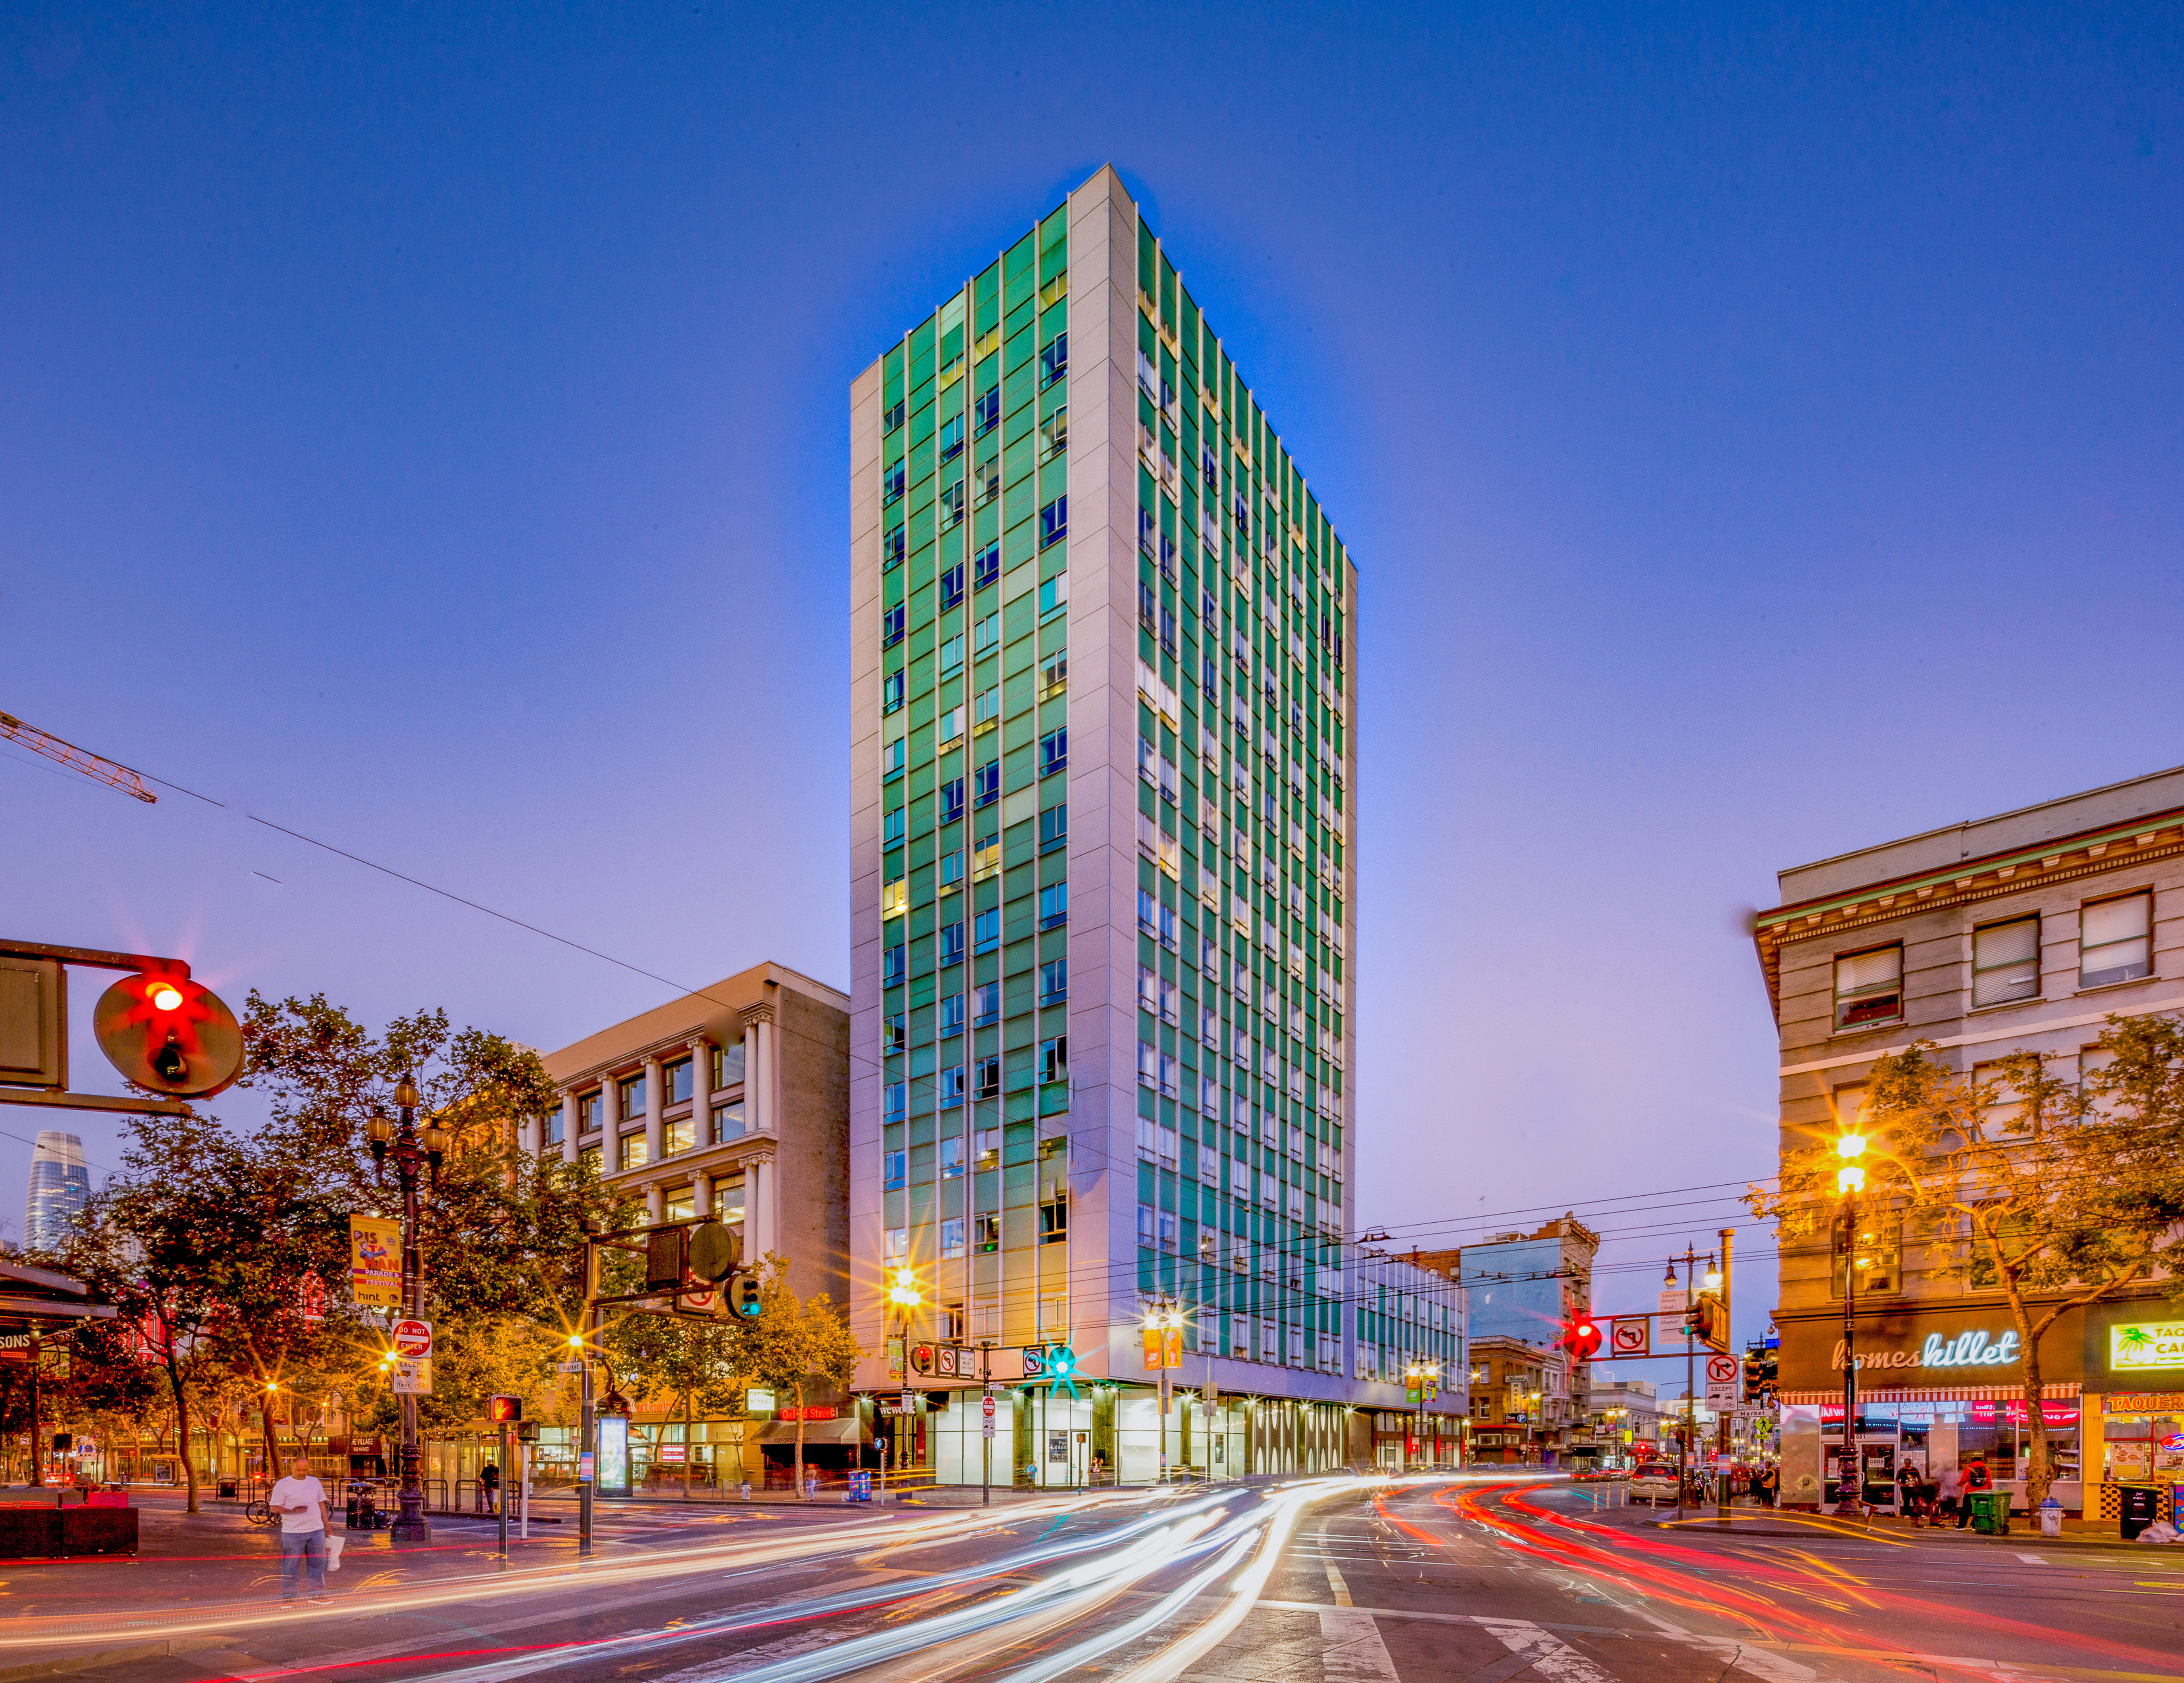
\includegraphics[width=\linewidth,height=52mm,keepaspectratio]{assets/history/frontier-tower-exterior.jpg}
      \par\smallskip
      {\tiny Frontier Tower, 995 Market Street\par
      Earlier exterior photo: \href{https://www.995market.com/}{Colliers / 995 Market listing}}
  \end{columns}
  \note{[03:00--03:30] I am a founding member of Biopunk Lab, working on synthetic neurobiology. I lead Neurotech@Frontier Tower, am co-founder of the Other Minds Lab, and am a lab member with Orthogonal Research and the DevoWorm Group, alongside my role as Executive Director of NeuroTechX. Membership and biographical details are supplied directly by Morgan; no dates, employment status, or additional project claims are inferred. The exterior image is an earlier property-listing photo of 995 Market Street, now Frontier Tower, not a photograph of current Frontier Tower activities.}
\end{frame}


\section{What is NeuroTechX?}
\NTXDivider{What is NeuroTechX?}
\begin{frame}{What is NeuroTechX?}
  \begin{columns}[T,onlytextwidth]
    \column{.52\textwidth}
      \NTXPoint{A nonprofit community}{Connecting neuroscience and technology.}
      \NTXPoint{Founded in Montr\'eal in 2015}{City chapters, student groups, and open source hardware and software projects.}
      \NTXPoint{Three pillars}{Community, education, and professional development.}
    \column{.43\textwidth}
      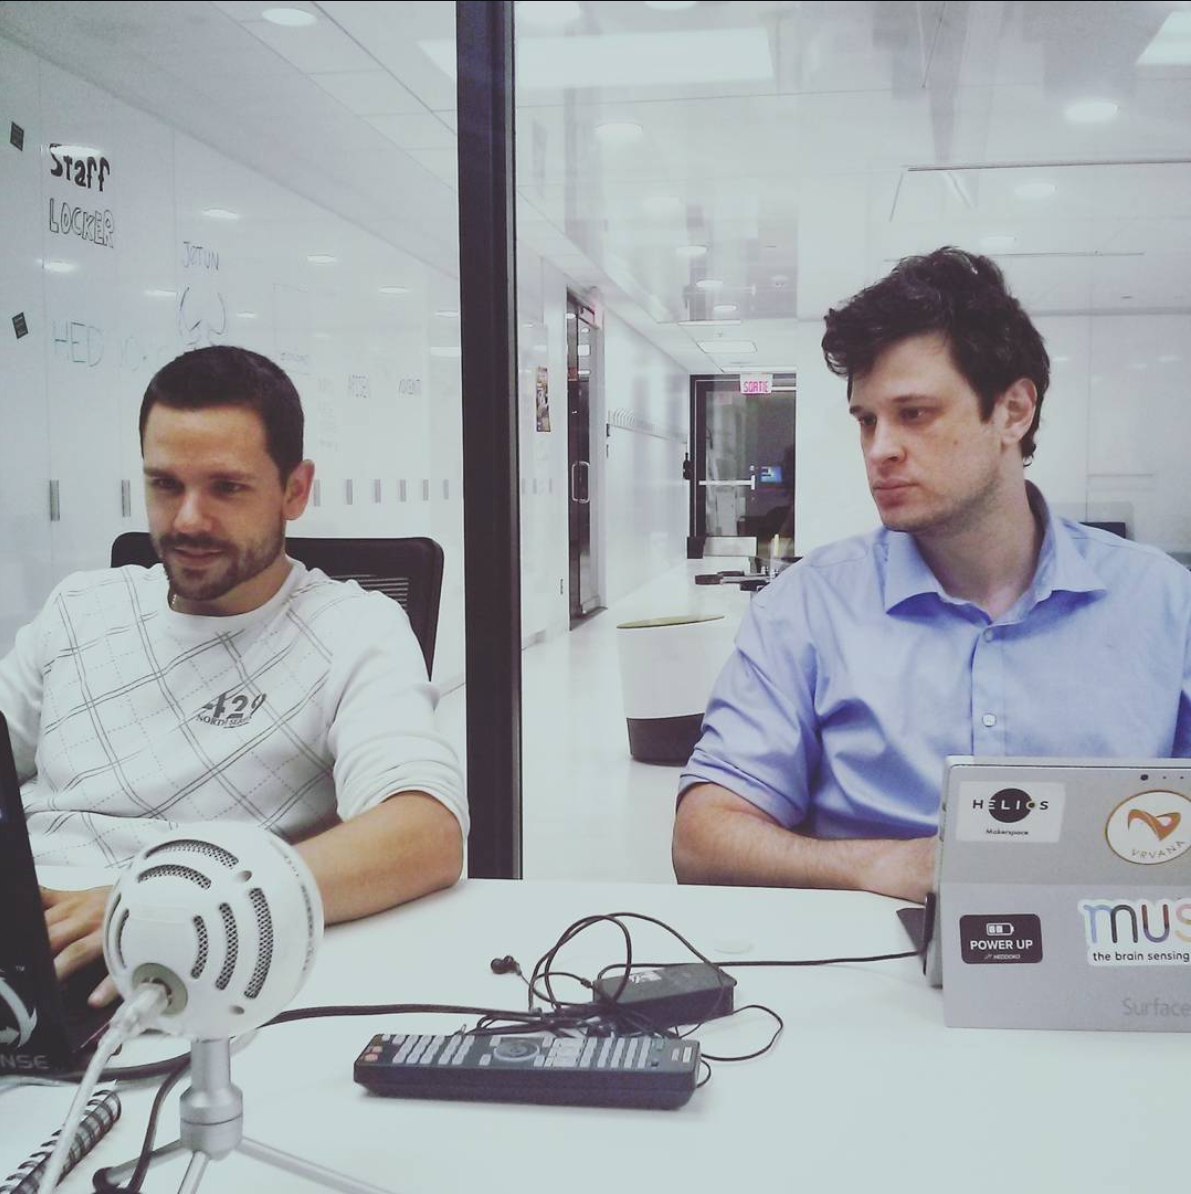
\includegraphics[width=\linewidth,height=47mm,keepaspectratio]{assets/people/neurotechx-instagram-1.png}
      \par\smallskip{\scriptsize Sydney Swaine-Simon and Yannick Roy\par}
  \end{columns}
  \NTXSource{https://www.neurotechx.org/about}{NeuroTechX: Our Story; photo from NeuroTechX's Instagram archive}
  \note{[03:30--04:30] Your original deck describes the organization as originally Societe BCI de Montreal and then a global community. The public history dates NeuroTechX's founding to 2015. Introduce the purpose without membership totals or superlatives. The exact legal history is not expanded beyond your supplied account.}
\end{frame}

\begin{frame}{What do we do?}
  \begin{columns}[c,onlytextwidth]
    \column{.43\textwidth}
      \small
      \NTXPoint{Community building}{Chapter meetings, hacknights, student chapters, hackathons, and student competitions.}
      \NTXPoint{Make learning accessible}{The NeuroTech Primer, workshops, webinars, and open science.}
      \NTXPoint{Build and share tools}{EEG-ExPy, MOABB, and contributions across open neurotechnology.}
    \column{.53\textwidth}
      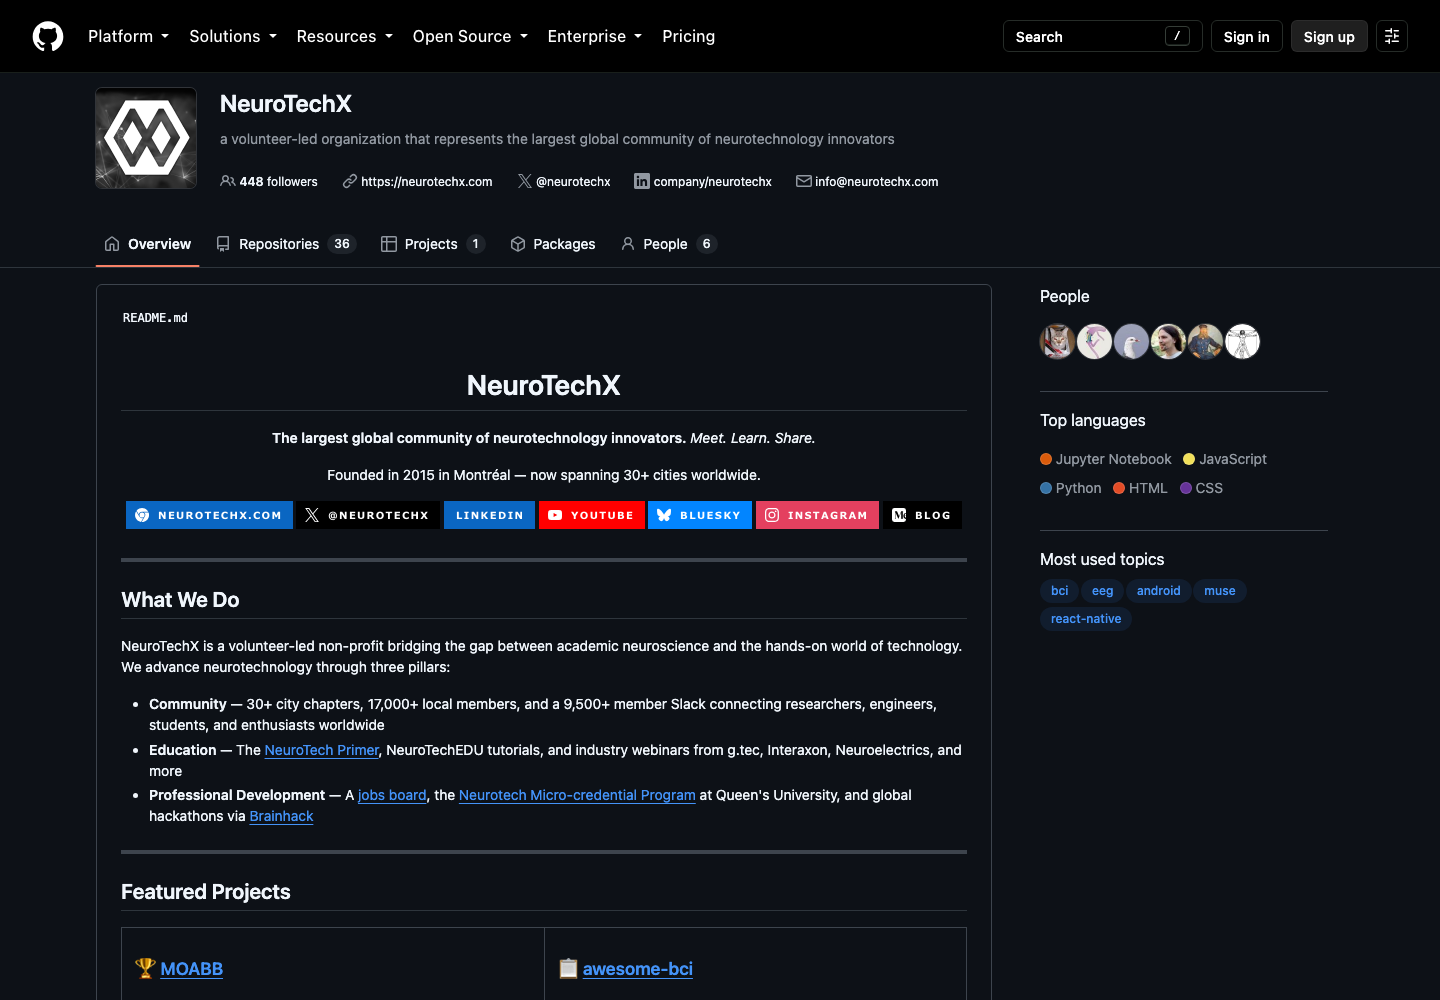
\includegraphics[width=\linewidth,height=49mm,keepaspectratio]{assets/history/neurotechx-github-org.png}
      \par\smallskip{\scriptsize \href{https://github.com/NeuroTechX}{github.com/NeuroTechX}\par}
  \end{columns}
  {\tiny\color{NTXMuted}Sources: \href{https://www.neurotechx.org/education}{NeuroTechX education}; GitHub organization homepage, captured September 6, 2026\par}
  \note{[04:30--05:30] This is the overview of the activities in your original slides. The next section makes each concrete. The image is an authentic logged-out screenshot of the NeuroTechX GitHub organization homepage, captured September 6, 2026. Point to the shared organization as a place where community work becomes accessible code and resources. Page counters and profile claims are a snapshot, not audited totals or additional claims in this talk. Distinguish NeuroTechX projects from independent tools our community uses or contributes to.}
\end{frame}

\section{What do we do?}
\NTXDivider{Community Building}
\begin{frame}{The first wave of BCI: control your world}
  \begin{columns}[c,onlytextwidth]
    \column{.61\textwidth}
      \small
      \NTXPoint{Consumer headsets opened the door}{Games, feedback, and device-control experiments made brain signals something people could explore outside a lab.}
      \NTXPoint{The promise brought people together}{Hardware to try, software to write, and results to compare: a starting point for hacknights and community building.}
      {\small\textbf{Early entry points}\par}
      {\small Muse \enspace EMOTIV \enspace NeuroSky \enspace OpenBCI\par}
      \medskip
      {\small\textbf{The ecosystem kept growing}\par}
      {\small Neurosity \enspace BrainBit \enspace Bitbrain \enspace MindAffect\par}
    \column{.35\textwidth}
      \centering
      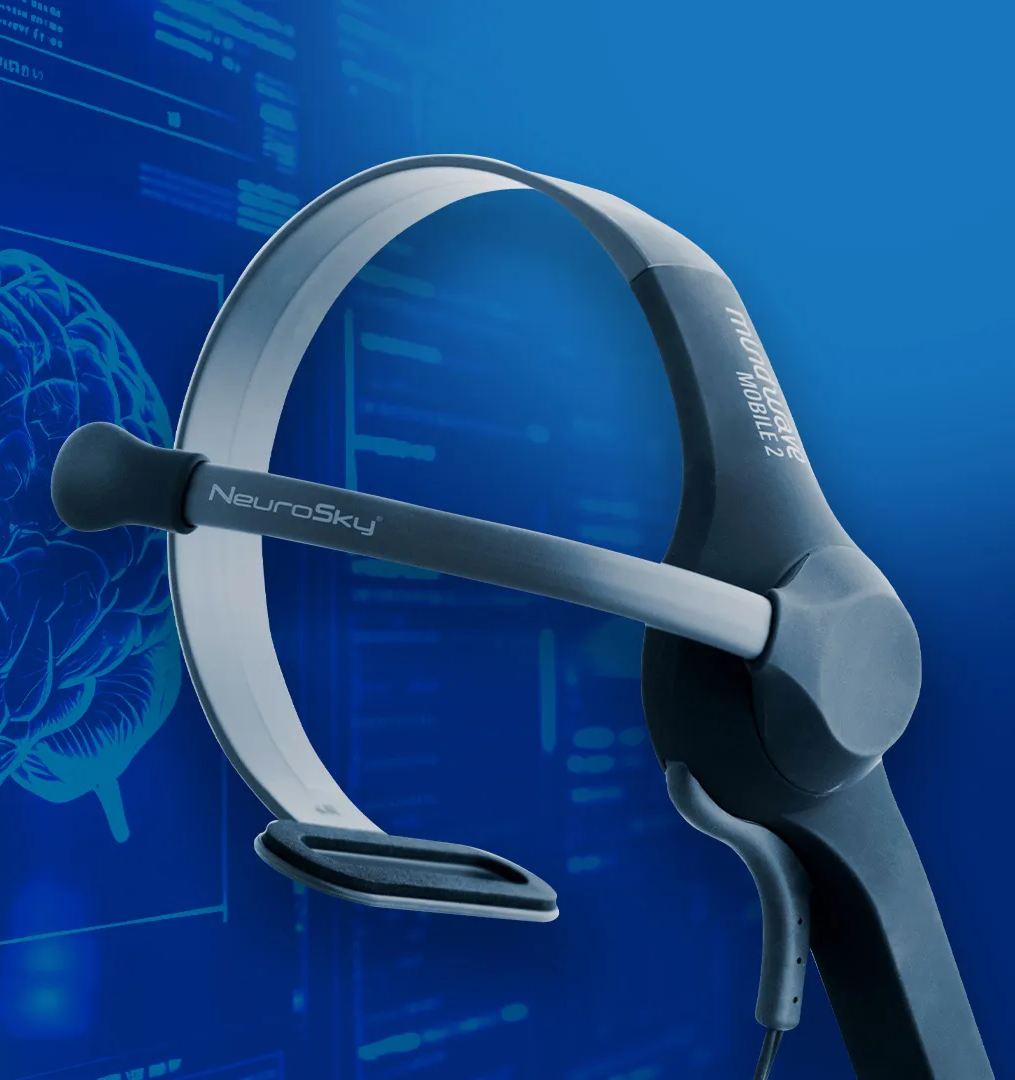
\includegraphics[width=\linewidth,height=40mm,keepaspectratio]{assets/history/neurosky-mindwave-mobile2.png}\par\smallskip
      {\tiny NeuroSky MindWave Mobile 2\newline Later model illustrating the headset lineage\newline Photo: NeuroSky\par}
  \end{columns}
  {\tiny\color{NTXMuted}Morgan's community-history framing. Sources: \href{https://www.emotiv.com/blog/how-emotiv-epoc-changed-the-world-of-neurotechnology}{EMOTIV}; \href{https://choosemuse.com/pages/team}{Muse}; \href{https://neurosky.com/neurosky-products/mindwave-headset/}{NeuroSky}; \href{https://openbci.com/community/openbci-on-kickstarter/}{OpenBCI}\par}
  \note{[05:30--07:00] Morgan's first wave means consumer and accessible non-invasive BCI driving community development, not the invention of BCI. The promise attracted people; making hardware work and understanding signals gave them a reason to learn together. Early milestones: EPOC in 2009, NeuroSky games and developer tools, OpenBCI's 2013 Kickstarter, and Muse's 2014 meditation-feedback launch. Muse was not primarily marketed for external device control. Neurosity, BrainBit, Bitbrain, and MindAffect represent the expanding ecosystem, not simultaneous launches or equal roles in NTX's founding. These span consumer products, open hardware, research devices, and BCI software, not interchangeable headsets. The MindWave Mobile 2 image depicts a later model. Control your world is an aspiration, not unrestricted thought reading, universal control, or clinical efficacy. No vendor sponsorship or formal partnership is implied. Transition to the chapter map. Detailed sources and boundaries: assets/history/first-wave-bci-sources.md.}
\end{frame}

\begin{frame}{A community across the world}
  \centering
  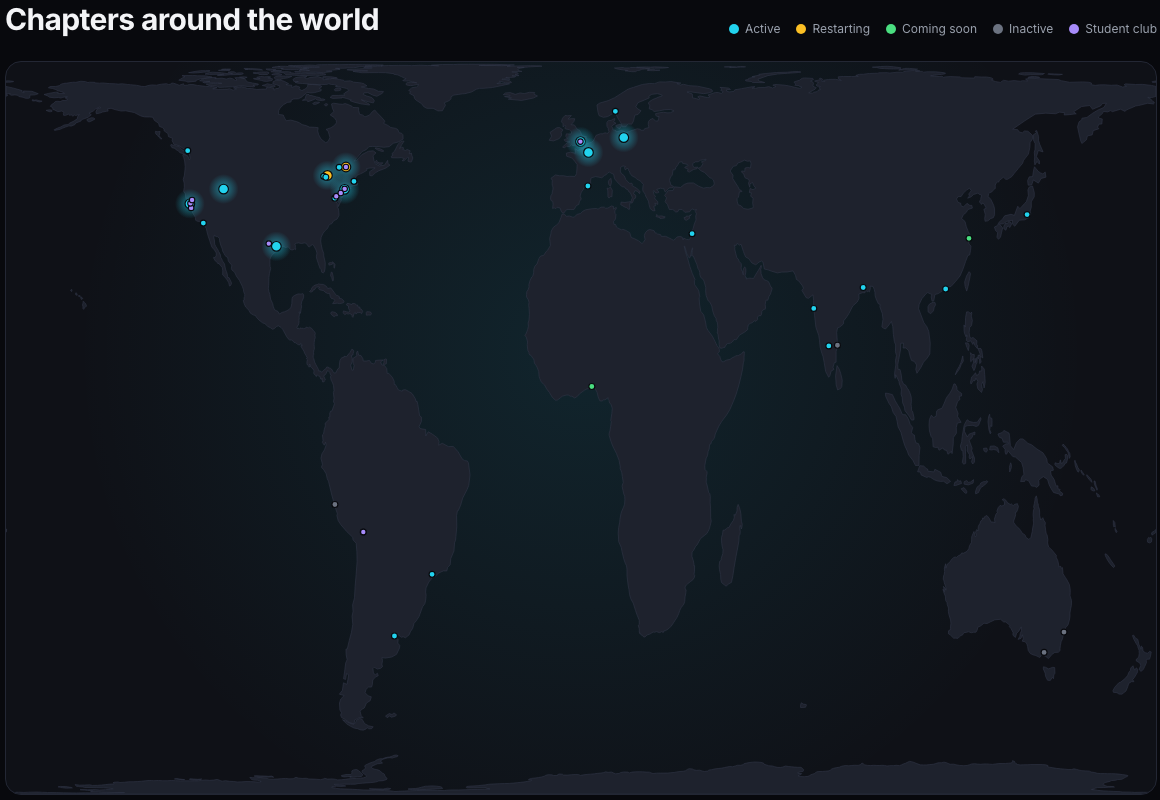
\includegraphics[width=\linewidth,height=55mm,keepaspectratio]{assets/chapters/neurotechx-community-map.png}
  \par\smallskip
  {\tiny\color{NTXMuted}\href{https://www.neurotechx.org/community}{NeuroTechX Community \& Chapters} --- website snapshot, September 6, 2026\par}
  \note{[07:00--07:30] Use the map to orient the audience before telling the local chapter histories. This is an authentic screenshot of the official community page, cropped to its map and original legend. It shows the geographic distribution of listings, not membership density or an audited count of active chapters. The legend distinguishes active, restarting, coming soon, inactive, and student club listings. A marker does not by itself establish that a chapter is currently running events.}
\end{frame}

\begin{frame}{Dans le vent}
  \framesubtitle{Local communities before NeuroTechX}
  \begin{columns}[T,onlytextwidth]
    \column{.47\textwidth}
      \textbf{San Francisco}\par\smallskip
      {\small Cognitive Technology Group\par}
      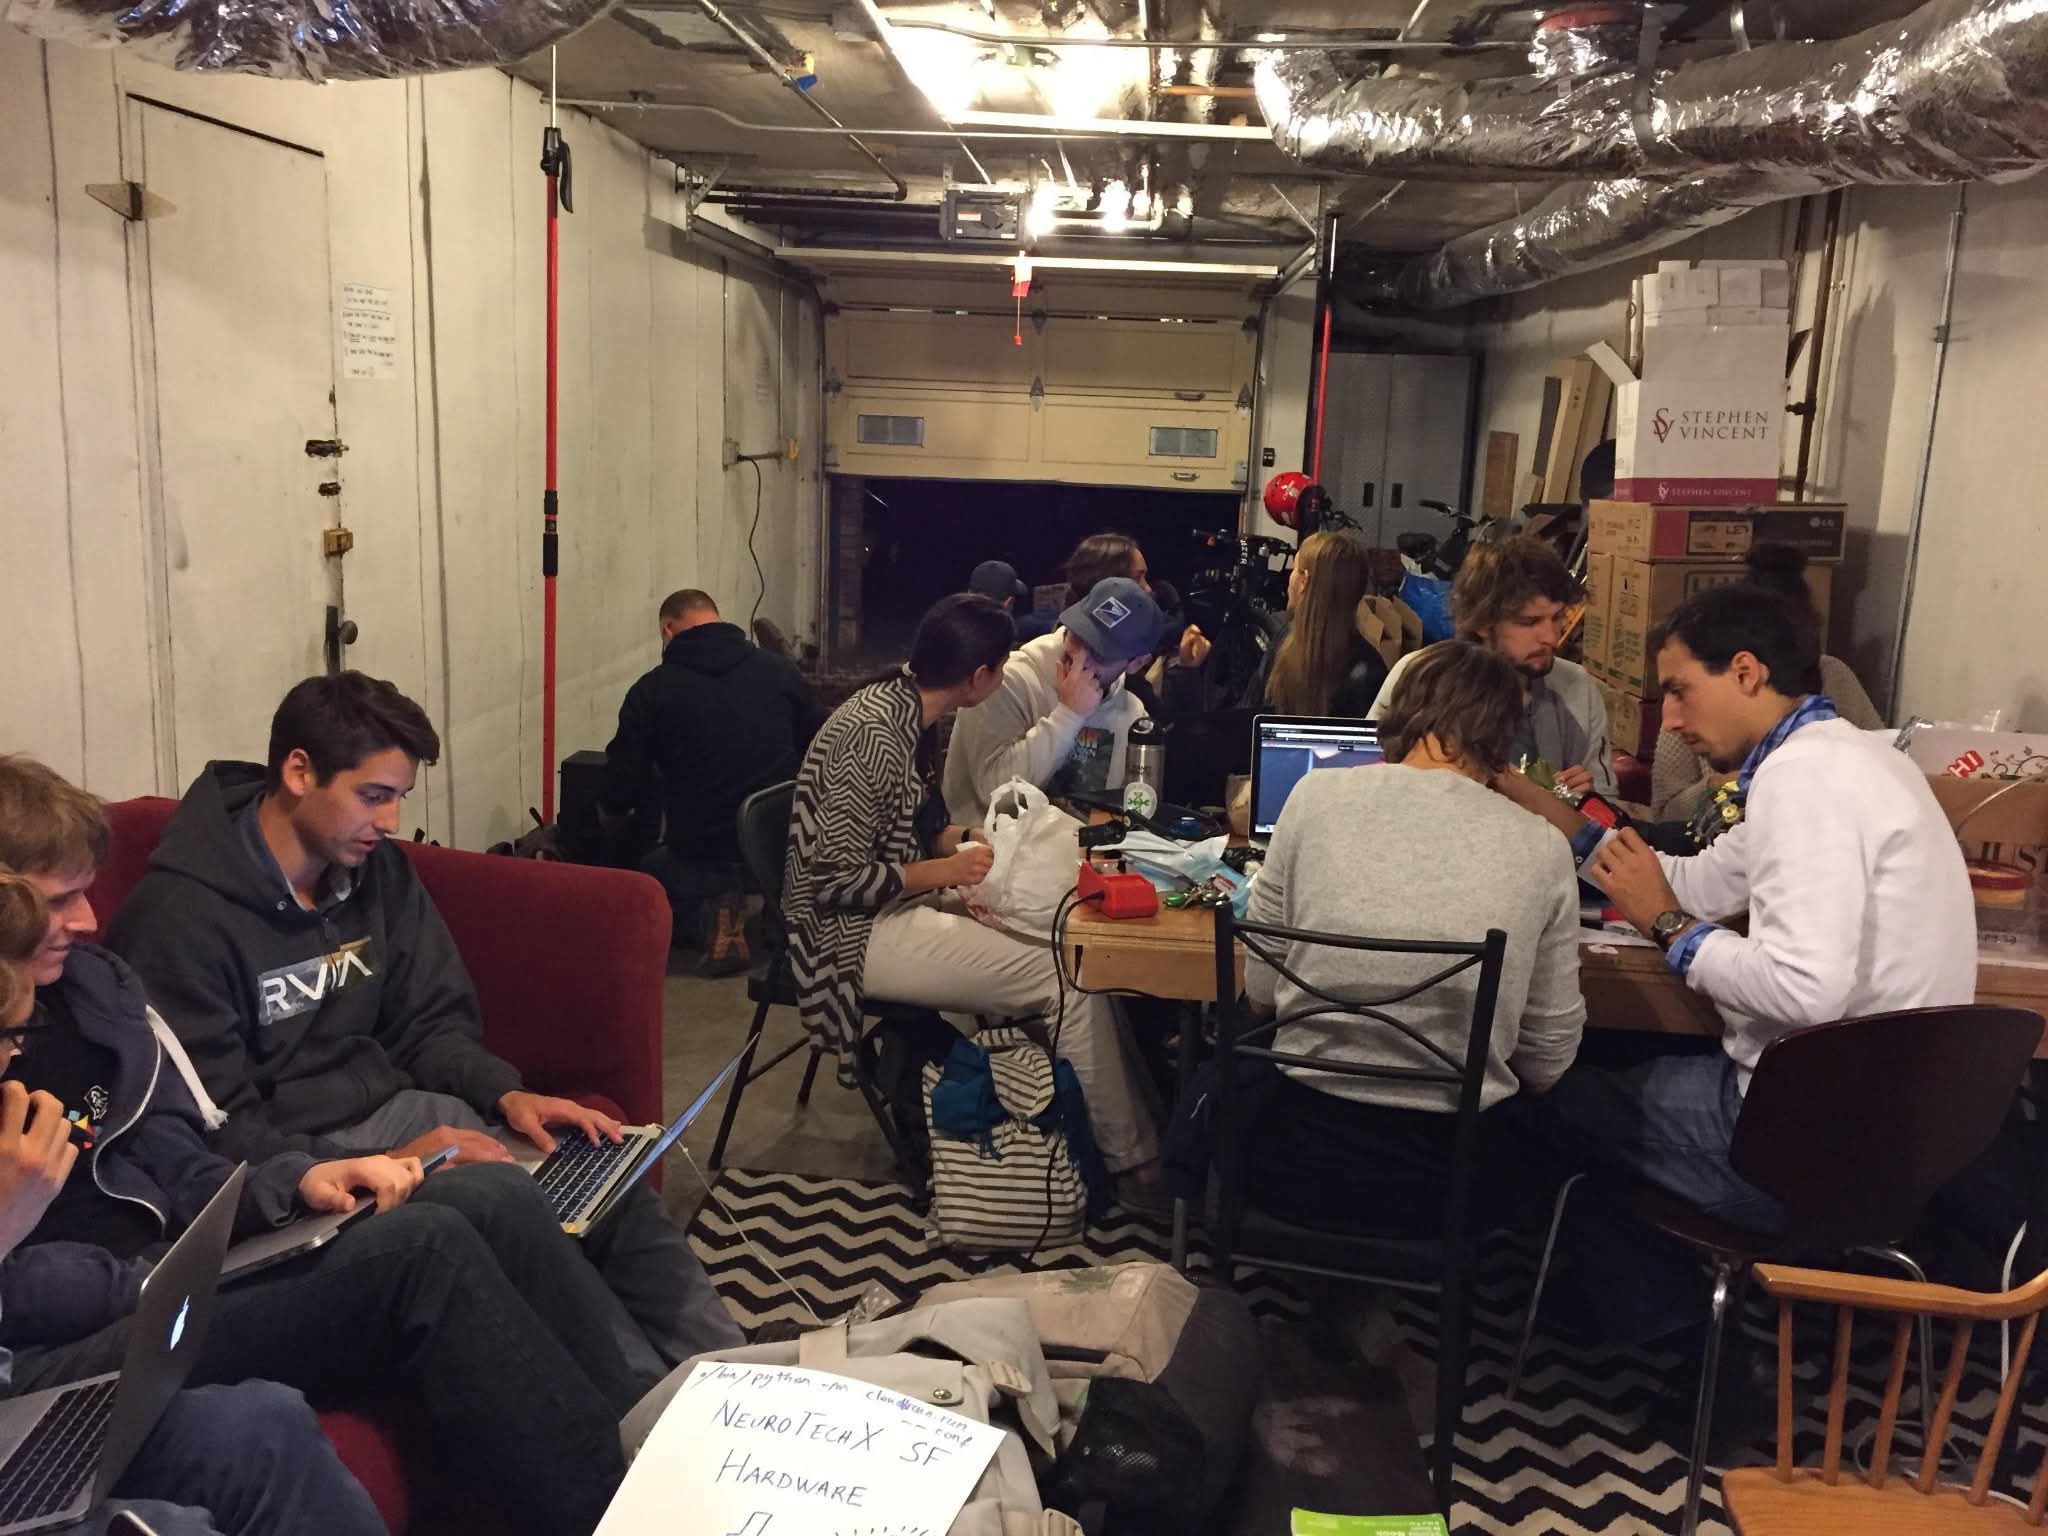
\includegraphics[width=\linewidth,height=28mm,keepaspectratio]{assets/chapters/san-francisco-original-hacknight.jpg}\par\smallskip
      {\small An existing community that became part of NeuroTechX\par}
      {\tiny Original SF Hacknights --- photo supplied by Morgan\par}
    \column{.47\textwidth}
      \textbf{Paris}\par\smallskip
      {\small CogLab --- September 2013\par}
      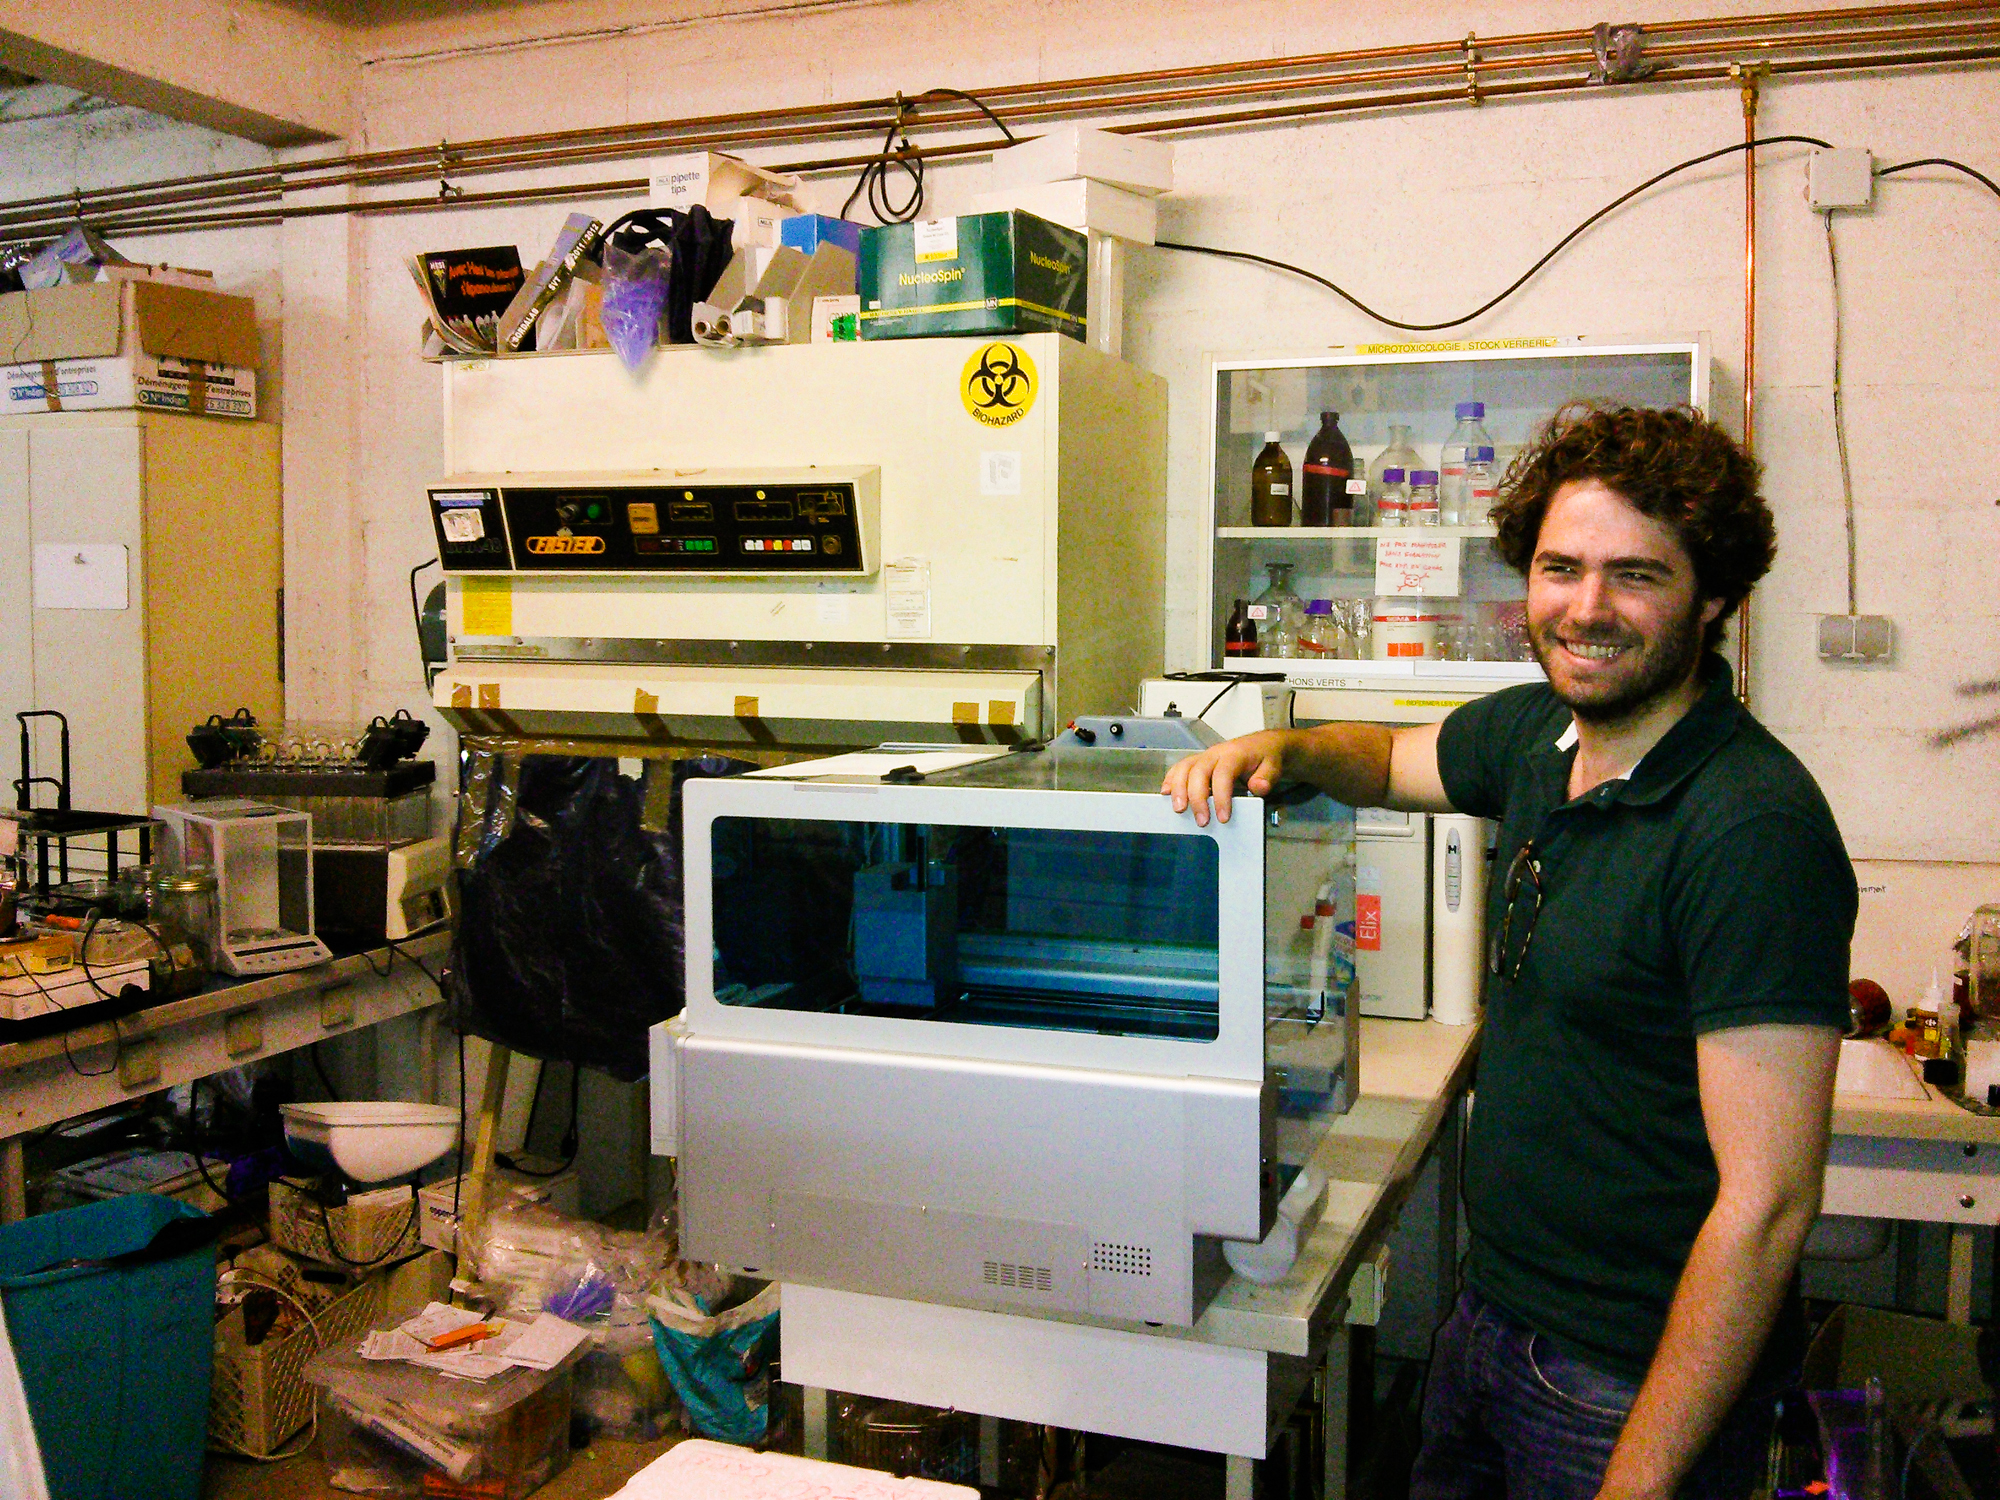
\includegraphics[width=\linewidth,height=28mm,keepaspectratio]{assets/chapters/la-paillasse-mitch-altman-2013.jpg}\par\smallskip
      {\small Launched by Romain Rouyer; incubated at La Paillasse\par}
      {\tiny La Paillasse, July 2013 --- \href{https://www.flickr.com/photos/maltman23/9379676390/}{Mitch Altman}, \href{https://creativecommons.org/licenses/by-sa/2.0/}{CC BY-SA 2.0}\par}
  \end{columns}
  {\tiny\color{NTXMuted}Sources: \href{https://github.com/Cognitive-Technology-Group}{Cognitive Technology Group archive}; \href{https://coglab.fr/about/coglab/}{CogLab: Gen\`ese}; Morgan Hough\par}
  \note{[07:30--08:15] Morgan identifies Cognitive Technology Group as the SF predecessor and CogLab as predating NeuroTechX Paris. CogLab's history dates its launch by Romain Rouyer to September 2013 and describes incubation at La Paillasse, collaboration with FRESCO and HackYourPhD, and accessible multidisciplinary experimentation. Morgan still cohosts Paris Hacknights. The SF archive contains EEG repositories created in 2014; these are not founding or affiliation dates. Neither chapter's formal transition date is asserted.}
\end{frame}

% Historical milestones, not an exhaustive chapter chronology.
\begin{frame}{San Francisco: overlapping communities, future founders}
  \begin{columns}[c,onlytextwidth]
    \column{.56\textwidth}
      \small
      \NTXPoint{Dream Team at Noisebridge}{I collaborated with the Dream Team and other groups forming around neurotech.}
      \NTXPoint{OpenBCI contributors to Neurosity founders}{AJ Keller / Push The World and Alex Castillo contributed firmware, drivers, and JavaScript tools before Neurosity.}
      \NTXPoint{Connections cross city boundaries}{AJ discovered OpenBCI through NeuroTechX; he and Alex met at a New York hackday in 2016.}
    \column{.40\textwidth}
      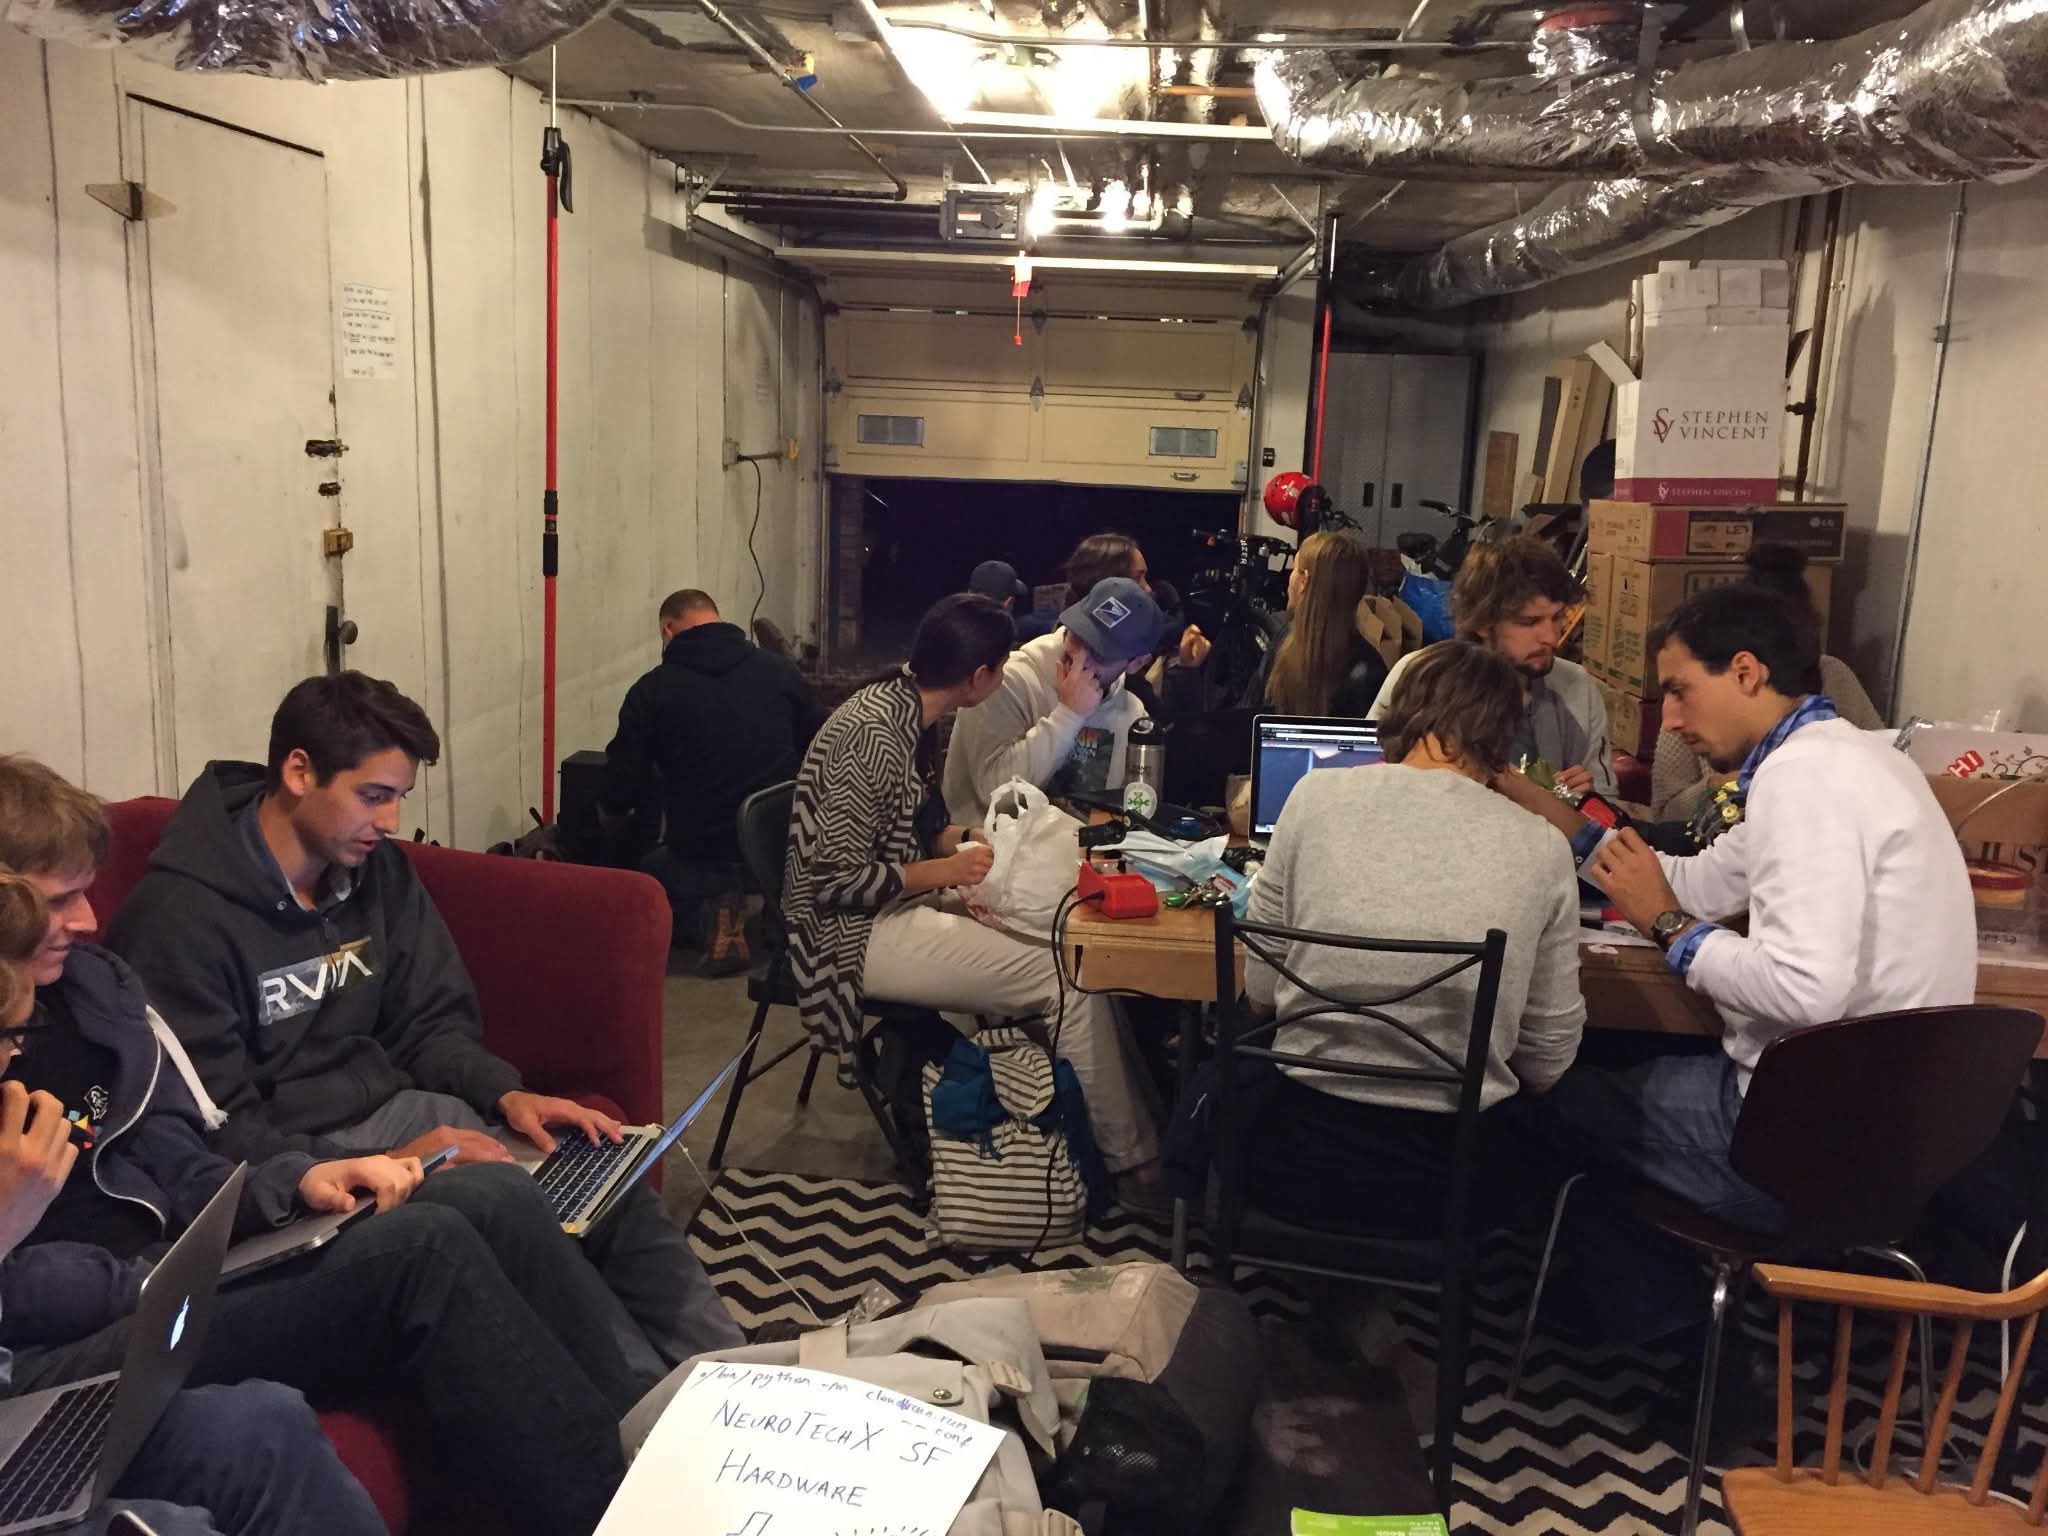
\includegraphics[width=\linewidth,height=39mm,keepaspectratio]{assets/chapters/san-francisco-original-hacknight.jpg}\par\smallskip
      {\tiny Original SF Hacknights / Morgan Hough\newline Community context, not a Dream Team event photo\par}
  \end{columns}
  {\tiny\color{NTXMuted}Sources: \href{https://www.noisebridge.net/wiki/DreamTeam}{DreamTeam}; \href{https://openbci.com/community/openbci-and-push-the-world/}{AJ Keller}; \href{https://openbci.com/community/new-javascript-open-source-projects-for-openbci/}{Alex Castillo, 2017}; \href{https://neurosity.co/about}{Neurosity}. Personal collaborations: Morgan Hough.\par}
  \note{[08:15--09:15] Morgan identifies his collaboration with the Dream Team at Noisebridge and other neurotech groups, and places Neurosity in his San Francisco ecosystem account. Noisebridge's indexed wiki describes DreamTeam as a neurohacking and AI experimentation group and lists OpenBCI, OpenEEG and other devices. AJ's OpenBCI guest post says he discovered OpenBCI through NeuroTechX. His later first-person account dates meeting Alex at an OpenBCI Friday hackday to 2016 and their shared Neurosity idea to 2018. OpenBCI's 2016 and 2017 records document Push The World's firmware and driver work; Alex's December 2017 JavaScript post thanks AJ. Distinguish New York origins of that collaboration from the later SF connection. No claim that Neurosity founded OpenBCI, that all named groups merged into NTX, or that Morgan collaborated personally with every founder. The photo is the existing SF Hacknight image, not identified as DreamTeam.}
\end{frame}

\begin{frame}{Toronto: learning together, building open tools}
  \begin{columns}[c,onlytextwidth]
    \column{.52\textwidth}
      \small
      \NTXPoint{Local roots: Steve Mann and InteraXon}{U of T's wearable and thought-controlled computing work; Ariel Garten's connection to Mann helped shape InteraXon's origins.}
      \NTXPoint{2016: learning and building together}{EEG lectures and biweekly Hacknights; open projects including EEG 101 and Neurodoro, in an ecosystem connected to InteraXon.}
      \NTXPoint{Student builders}{NeuroTechUofT's 2016 demo: VitReous, an eye-gesture interface for VR/AR.}
    \column{.43\textwidth}
      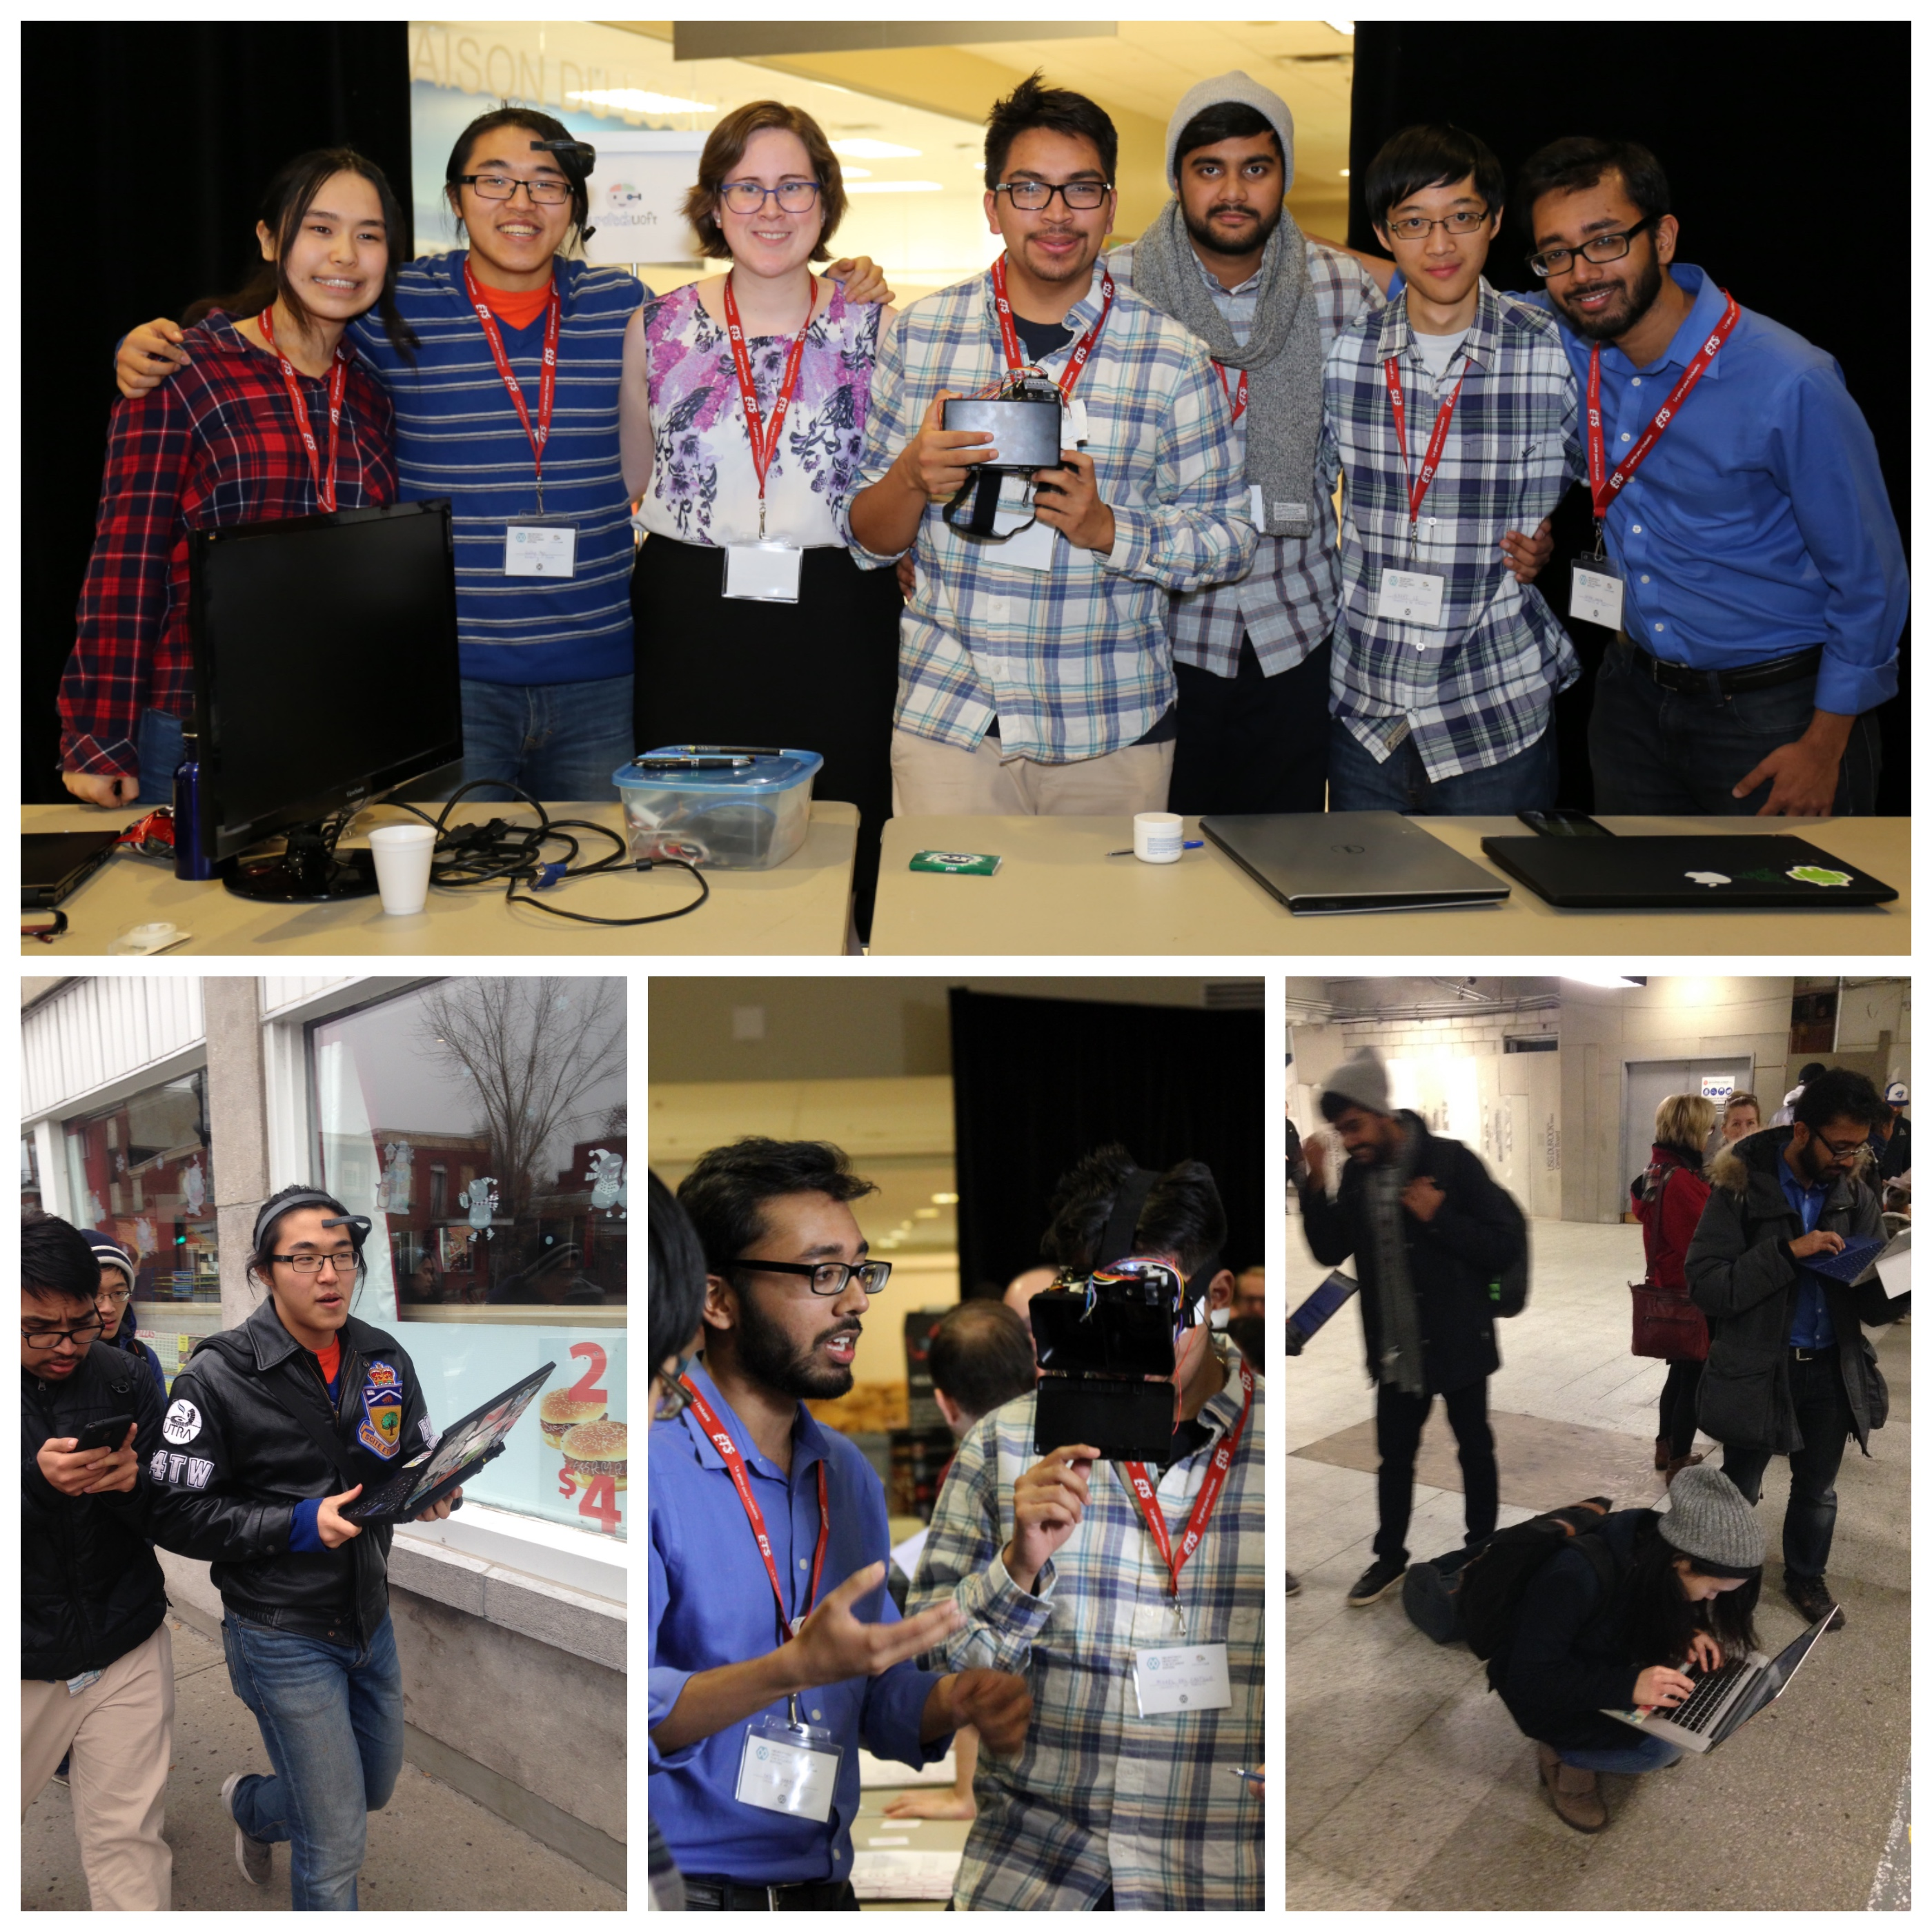
\includegraphics[width=\linewidth,height=48mm,keepaspectratio]{assets/chapters/toronto-student-demo-2016.jpg}
      \par\smallskip{\scriptsize NeuroTechUofT --- Student Demo Day, 2016\par}
  \end{columns}
  {\tiny\color{NTXMuted}Sources: \href{https://news.engineering.utoronto.ca/thought-control-technology-can-make-toast/}{U of T, 2010}; \href{https://www.ece.utoronto.ca/people/mann-s/}{Steve Mann}; \href{https://neurotechx.com/chapter/1531/}{Toronto chapter}; \href{https://neurotechx.github.io/studentclubs/news/student-clubs-2016/}{student archive / photo}\par}
  \note{[09:15--10:15] Toronto's community sits in a longer local history. U of T's August 2010 account connects InteraXon CEO Ariel Garten with her former teacher Steve Mann and his thought-controlled computing work. Mann's faculty profile documents his wearable-computing and EyeTap research. Distinguish this technology lineage from the chapter's own founding: neither Mann nor InteraXon is asserted to have founded NTX Toronto. The chapter archive names connections with InteraXon, Avertus and the Ontario Brain Institute, and describes biweekly Hacknights and open mobile projects. The February 2016 NTX Digest records January's EEG lectures. The image is NeuroTechUofT's 2016 student Demo Day, not a Mann or InteraXon demonstration. VitReous used EOG eye gestures, not EEG decoding. EEG 101 is historical: its repository was archived in 2021 after loss of Muse SDK support. The lesson is the interplay of university research, local companies, and community-led learning.}
\end{frame}

\begin{frame}{New York: from Hacknights to NeuroNYC meetings}
  \begin{columns}[c,onlytextwidth]
    \column{.52\textwidth}
      \small
      \NTXPoint{2015: an early NeuroTechX community}{Conor Russomanno's organizing history begins in July; monthly Hacknights around human--computer interfaces.}
      \NTXPoint{2016: prototype testing together}{Dark Maze was tested at a NeuroTechNYC meetup using OpenBCI.}
      \NTXPoint{2025--26: NeuroNYC meetings}{Happy hours, NeuroBall, a summer summit, and a foundation-models symposium connect today's ecosystem.}
    \column{.43\textwidth}
      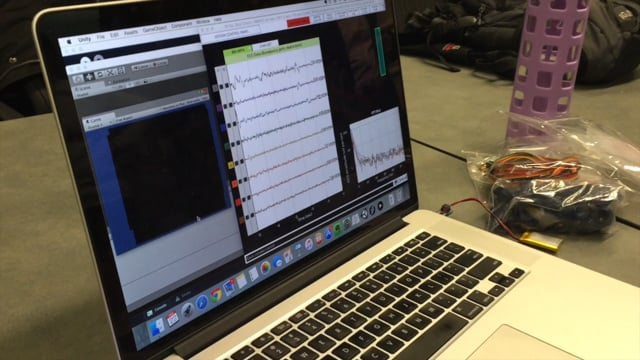
\includegraphics[width=\linewidth,height=23mm,keepaspectratio]{assets/chapters/new-york-darkmaze-2016.jpg}
      \par{\tiny Dark Maze meetup test, 2016 / Mathura\par}\smallskip
      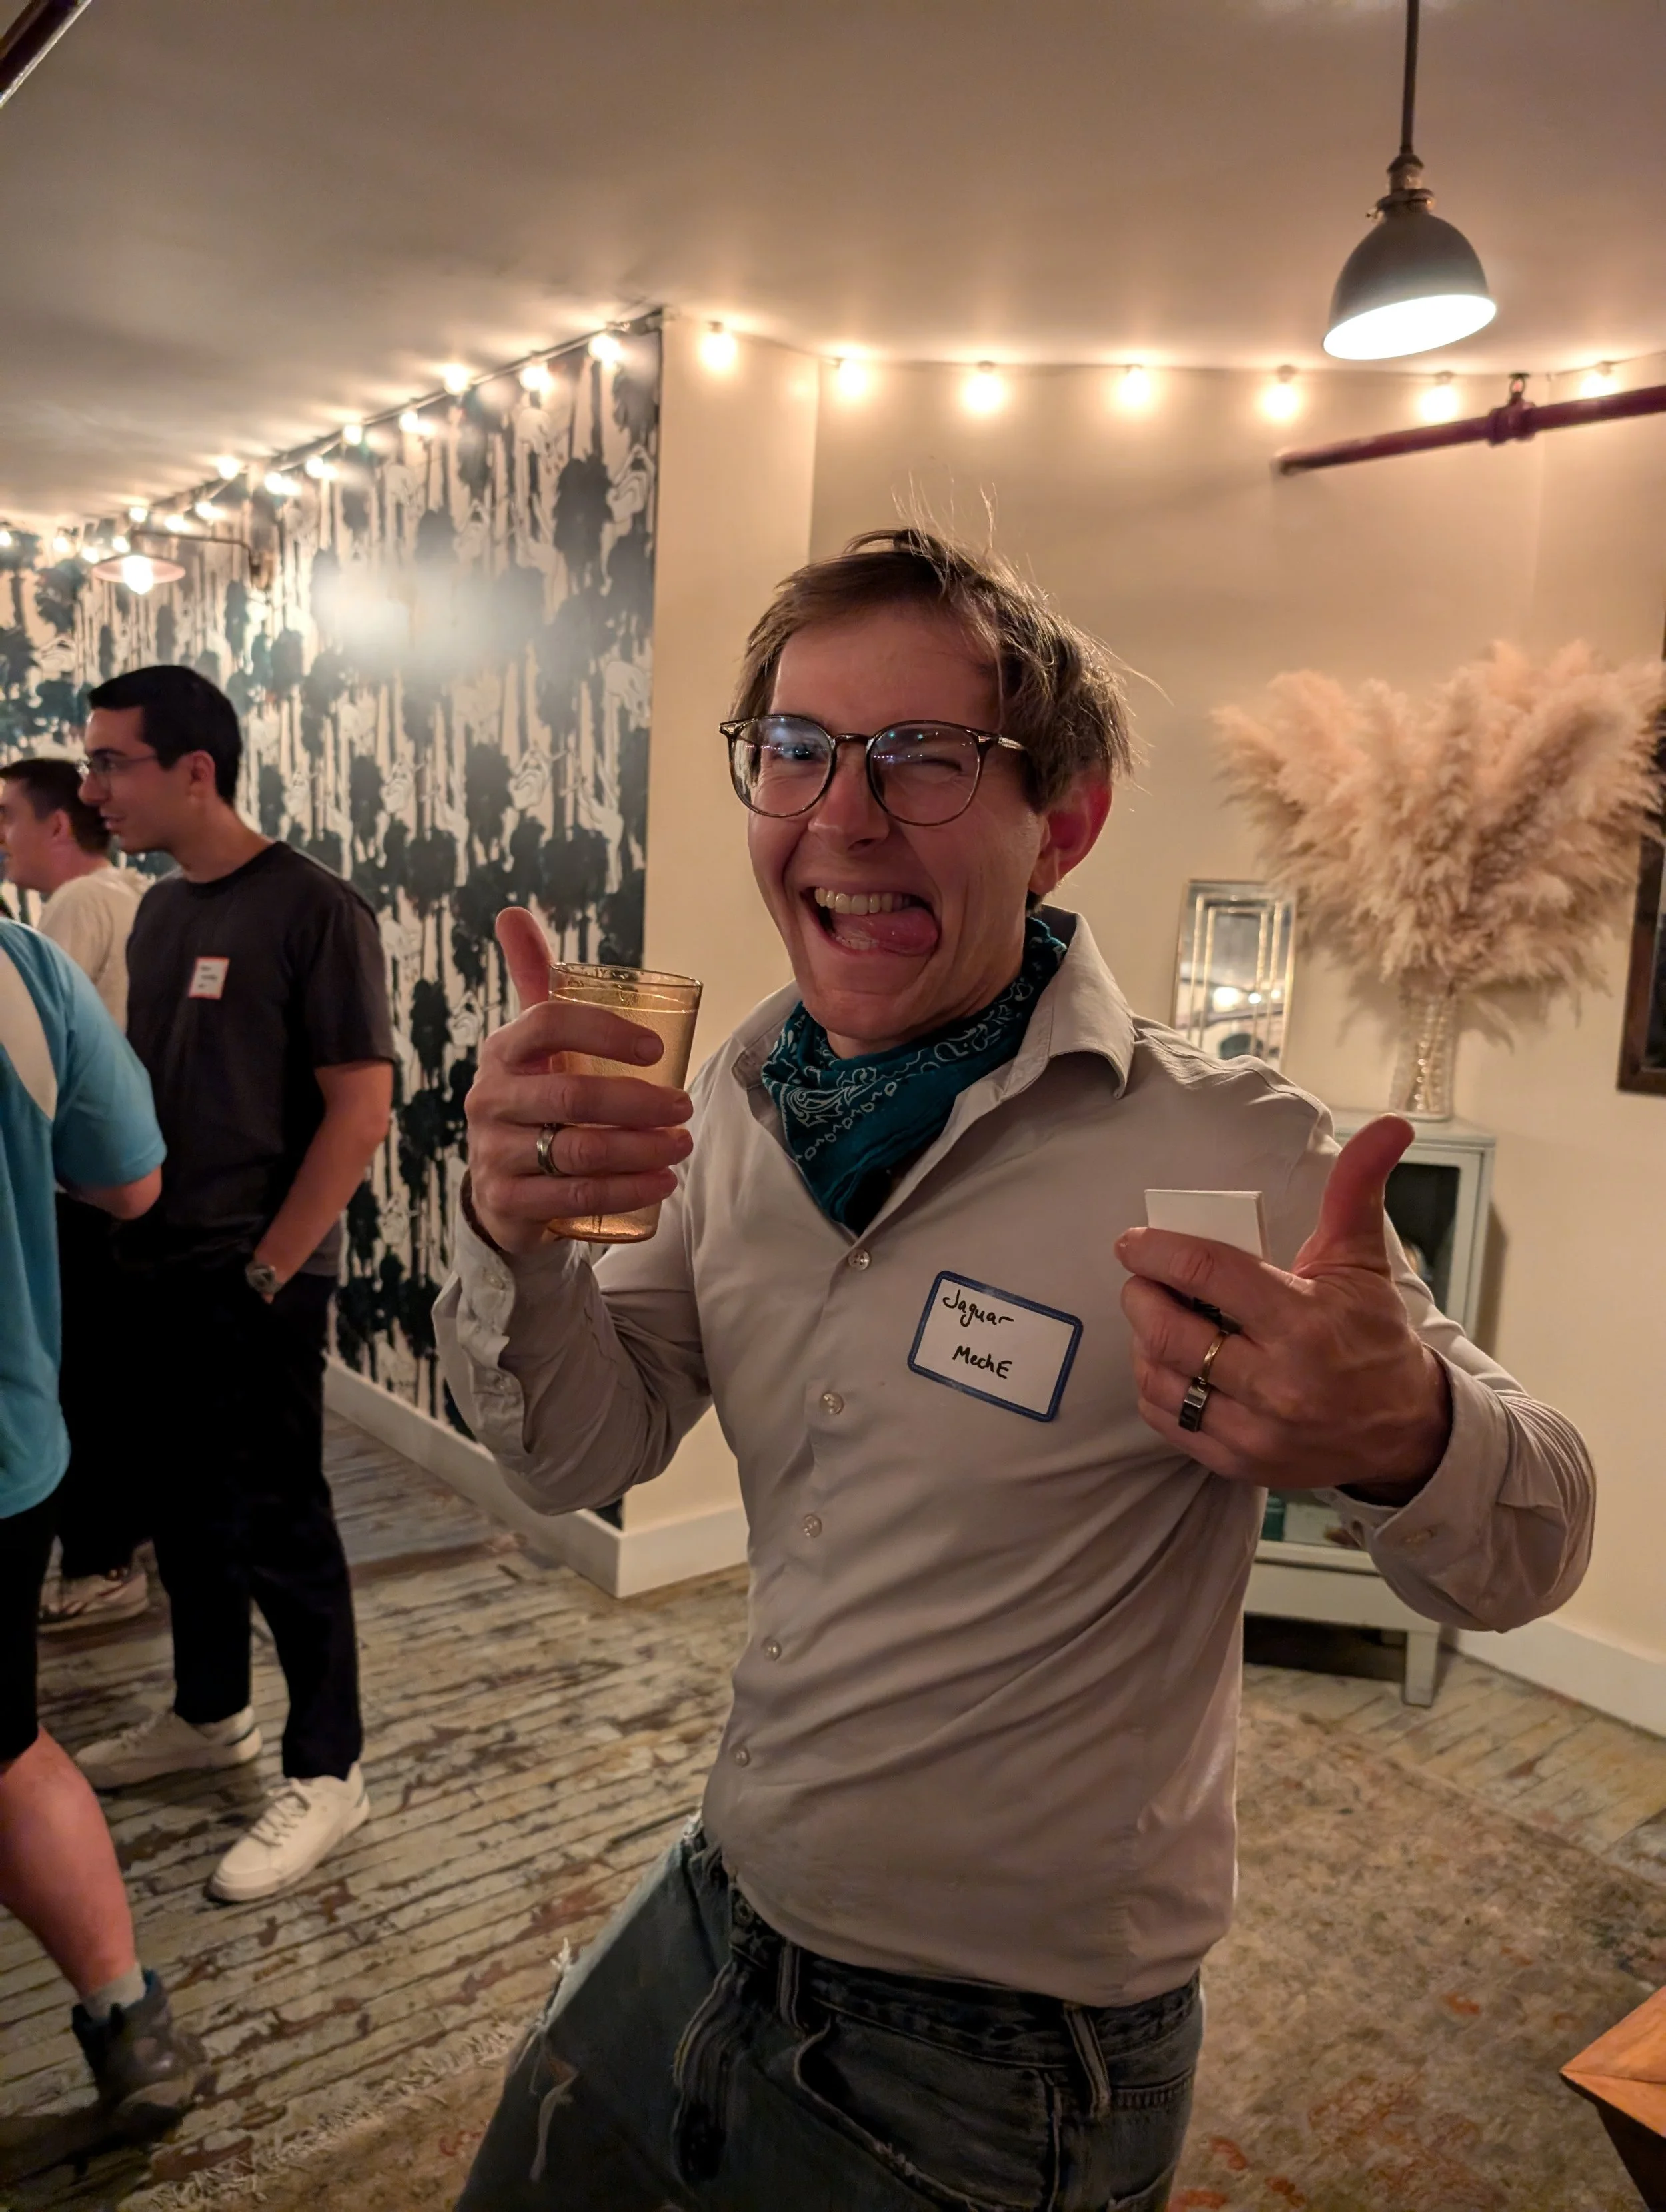
\includegraphics[width=\linewidth,height=23mm,keepaspectratio]{assets/chapters/neuronyc-calendar-meeting.png}
      \par{\tiny NeuroNYC meeting / official event-gallery photo\par}
  \end{columns}
  {\tiny\color{NTXMuted}Sources: \href{https://conorrussomanno.com/}{Conor Russomanno}; \href{https://mathuramg.com/projects/darkMaze.html}{Mathura: Dark Maze}; \href{https://neuro-nyc.org/calendar}{NeuroNYC events / photo}. Historical groups and current organizers are distinct.\par}
  \note{[10:15--11:15] Conor Russomanno dates his NeuroTechNYC organizing to July 2015. Dark Maze was tested at a meetup, documented by Mathura's February 2016 video; the thumbnail is shown above. Neural-network EEG teaching continued in a documented April 2018 Hacknight. The lower photo comes from NeuroNYC's current event gallery; its filename suggests October 2024, but no precise event date is asserted. The newer calendar documents NeuroBall in December 2025, a March 26, 2026 foundation-models symposium and a July 2026 summer summit. The summit calendar header and description disagree on the day, so only the month is used in our source notes. Present this as a continuing city ecosystem, not evidence of a legal merger, rebrand, or current NTX affiliation. The September 10, 2026 Precision Neuroscience careers event remains upcoming at the time of this talk.}
\end{frame}

\begin{frame}{Boston: founders, public dialogue, and community}
  \begin{columns}[c,onlytextwidth]
    \column{.55\textwidth}
      \small
      \NTXPoint{Chapter roots and local founders}{NTX Boston from 2016; Neurable's Ramses Alcaide and Adam Molnar in the local ecosystem.}
      \NTXPoint{2022: public conversation}{Adam joined the NTX Boston / BrainMind neuroethics panel at MIT.}
      \NTXPoint{2025: a successor gathering}{Augmentation Lab's Human Augmentation Summit, August 23, MIT Media Lab: demos, talks, and hands-on exhibits.}
    \column{.41\textwidth}
      \centering
      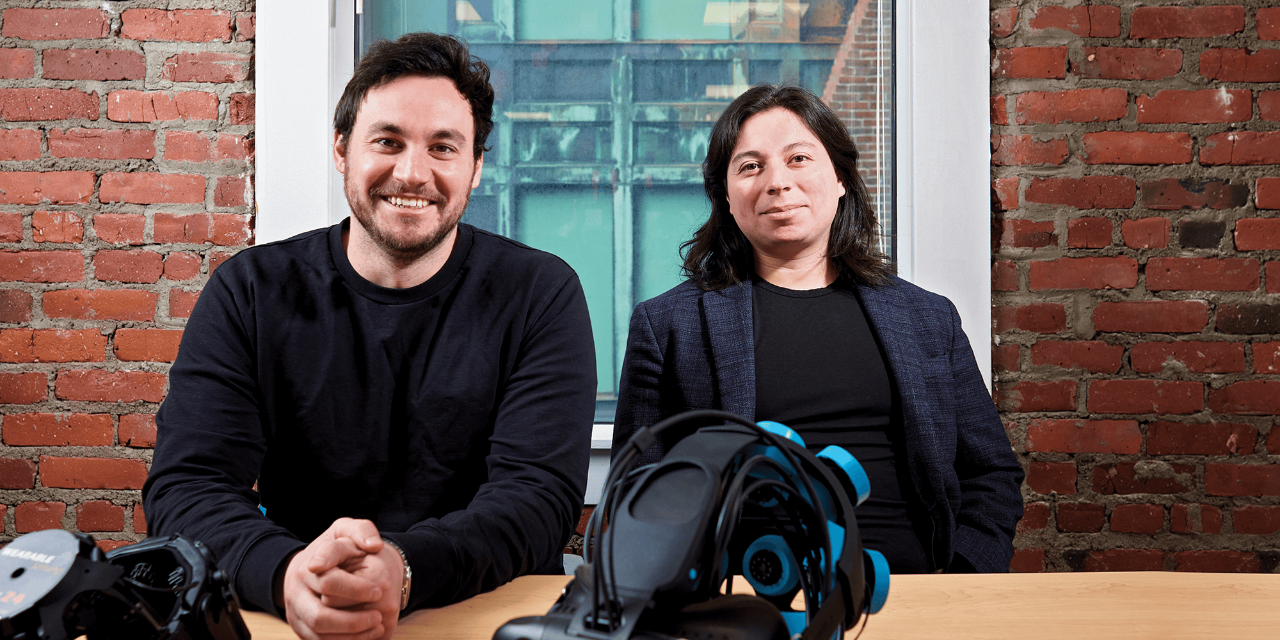
\includegraphics[width=\linewidth,height=22mm,keepaspectratio]{assets/chapters/boston-neurable-founders.png}
      \par{\tiny Adam Molnar (left), Ramses Alcaide (right)\newline Neurable HQ --- Philip Keith Photography / U-M\par}\smallskip
      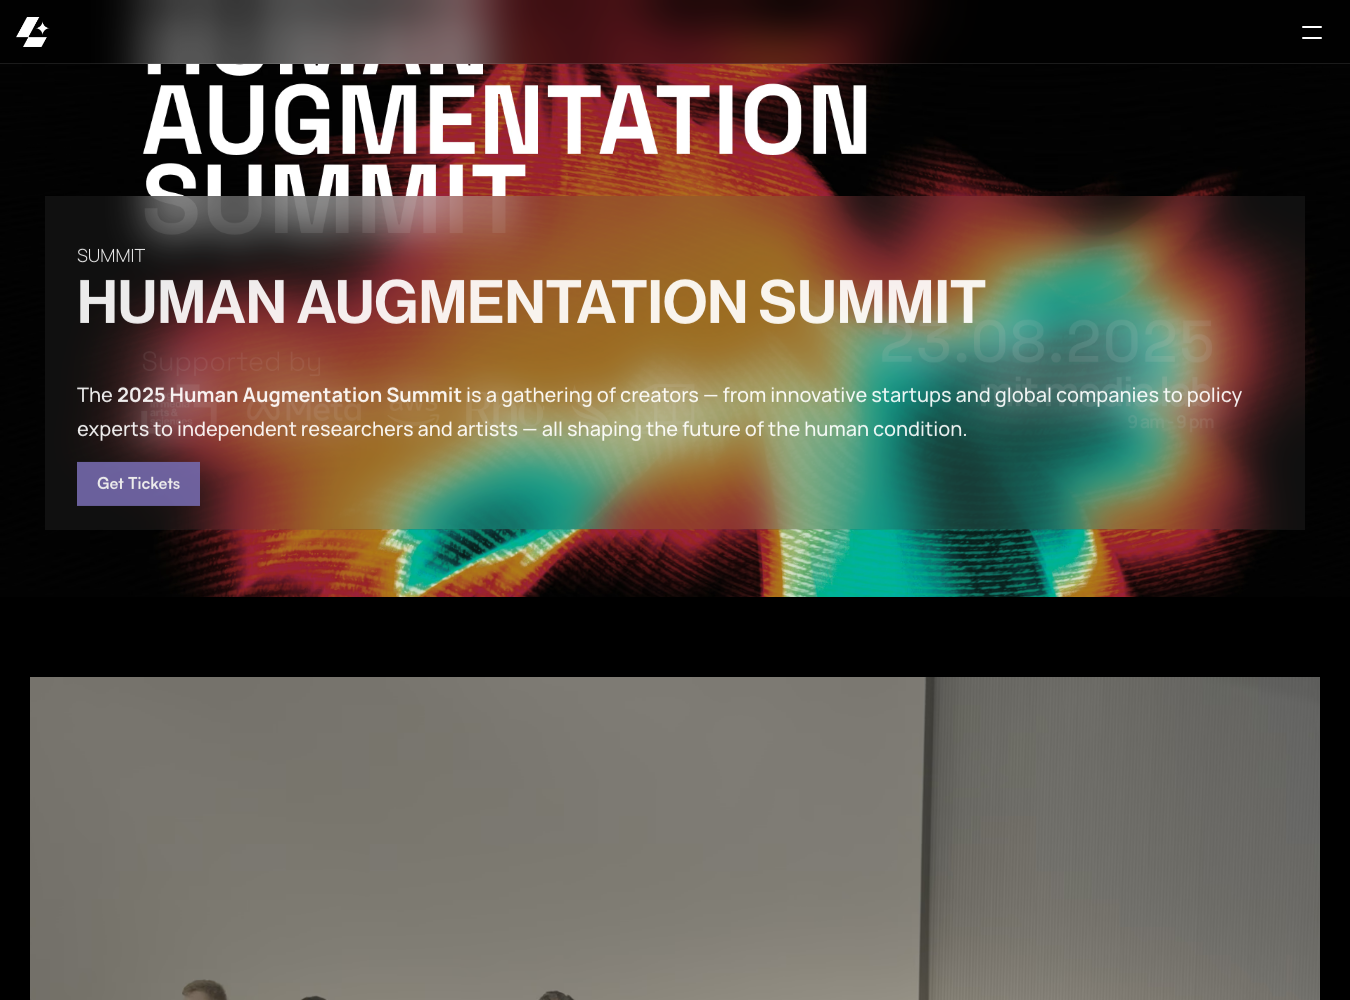
\includegraphics[trim=0 300 0 0,clip,width=\linewidth,height=22mm,keepaspectratio]{assets/history/augmentation-summit-2025-page.png}
      \par{\tiny Official 2025 summit page / Augmentation Lab\par}
  \end{columns}
  {\tiny\color{NTXMuted}Sources: \href{https://neurotechx.com/chapter/1543/}{Boston chapter}; \href{https://www.neurable.com/blog-posts/were-neurable-nice-to-meet-you}{Neurable}; \href{https://augmentationlab.org/summit}{Augmentation Lab summit}. Successor-community framing: Morgan Hough.\par}
  \note{[11:15--12:45] Boston's chapter roots date to 2016. Neurable founders Ramses Alcaide and Adam Molnar are part of the local ecosystem, not established NTX chapter founders. The upper photograph is from U-M's Spring 2023 feature, credited to Philip Keith Photography at Neurable's Boston HQ. Adam joined the June 29, 2022 NTX Boston/BrainMind neuroethics panel at MIT; Alex Higuera was credited for organizing. Morgan identifies Augmentation Lab's 2025 meeting as a successor gathering in this community history. The official page verifies the Human Augmentation Summit on August 23, 2025 at MIT Media Lab in Cambridge, with demos, talks, panels and exhibits. Successor means continuation of local community energy, not an independently verified organizational transfer or NTX ownership. The lower image is the official summit page, not a photograph proving attendance. Boston/London Buzz-in-Review history is retained elsewhere.}
\end{frame}

\begin{frame}{London: connecting research, makers, and students}
  \begin{columns}[c,onlytextwidth]
    \column{.52\textwidth}
      \NTXPoint{May 2016: first meetup at LSE}{With the NERRI project; three-minute talks designed for non-specialists.}
      \NTXPoint{2022: a shared London--Boston event}{Hybrid Buzz-in-Review linked two local communities.}
      \NTXPoint{2025: student-led building}{London Neurotech Hackathon with Imperial's Neurotech Society and partners including NeuroTechX.}
    \column{.43\textwidth}
      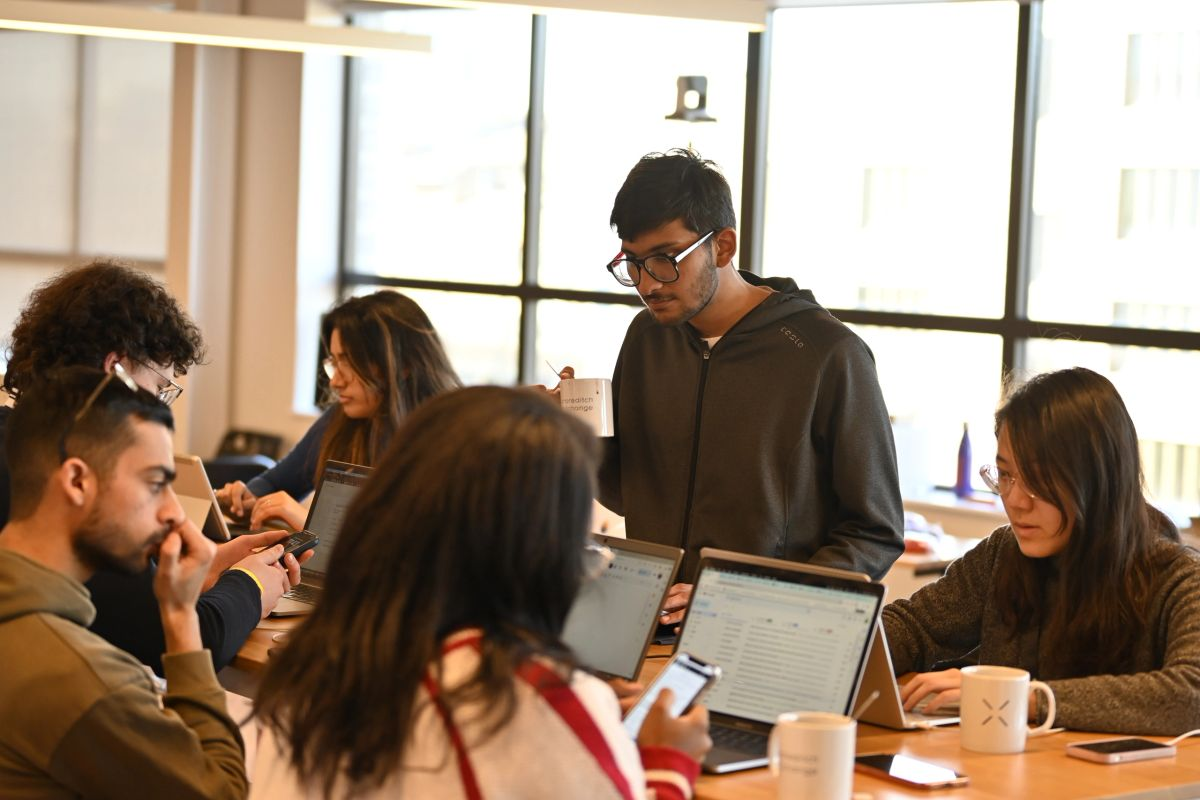
\includegraphics[width=\linewidth,height=43mm,keepaspectratio]{assets/chapters/london-hackathon-2025.jpg}
      \par\smallskip{\scriptsize London Neurotech Hackathon, January 2025\par Photo: Imperial College Neurotech Society\par}
  \end{columns}
  {\tiny\color{NTXMuted}Sources: \href{https://www.meetup.com/NeuroTechLDN/events/230512143/}{May 6, 2016 meetup}; \href{https://www.linkedin.com/posts/ben-woodington_neurotechx-ldn-bos-buzz-in-review-2022-activity-6894574014426398720-_Ash}{2022 organizer announcement}; \href{https://iclneurotech.co.uk/hackathon}{2025 organizer recap / photo}\par}
  \note{[12:45--13:45] The original Meetup listing identifies May 6, 2016 at LSE's New Academic Building as the first London chapter meetup, supported by the NERRI project. Hosts were Javier Asensio and Imre Bard. Its flash-talk format explicitly invited accessible introductions for non-academics, with research, startups, Cybathlon, and London Hackspace Brain Hackers represented. Ben Woodington's announcement describes a February 5, 2022 hybrid Buzz-in-Review shared with Boston, with London's in-person gathering at Bellavita Academy. The image is from Imperial College Neurotech Society's January 25--26, 2025 hackathon recap, which explicitly credits NeuroTechX among its partners. It is not a photograph of the 2016 or 2022 meeting. Avoid the conflicting 30/36-hour descriptions and unverified first-ever superlatives. The thread is continuity through collaborations between local organizers, researchers, makers, and students.}
\end{frame}

\begin{frame}{India: building community across distance}
  \begin{columns}[c,onlytextwidth]
    \column{.58\textwidth}
      \NTXPoint{October 2020: Neuro 2.0}{A two-day online forum connecting the India community with international speakers.}
      \NTXPoint{January 2021: shared Buzz-in-Review}{India and Australia paired in the global chapter program.}
      \NTXPoint{September 2021: India's own ecosystem}{A discussion with Eywa Neuro on invasive BMI, microelectrodes, and bioMEMS manufacturing.}
    \column{.35\textwidth}
      \centering
      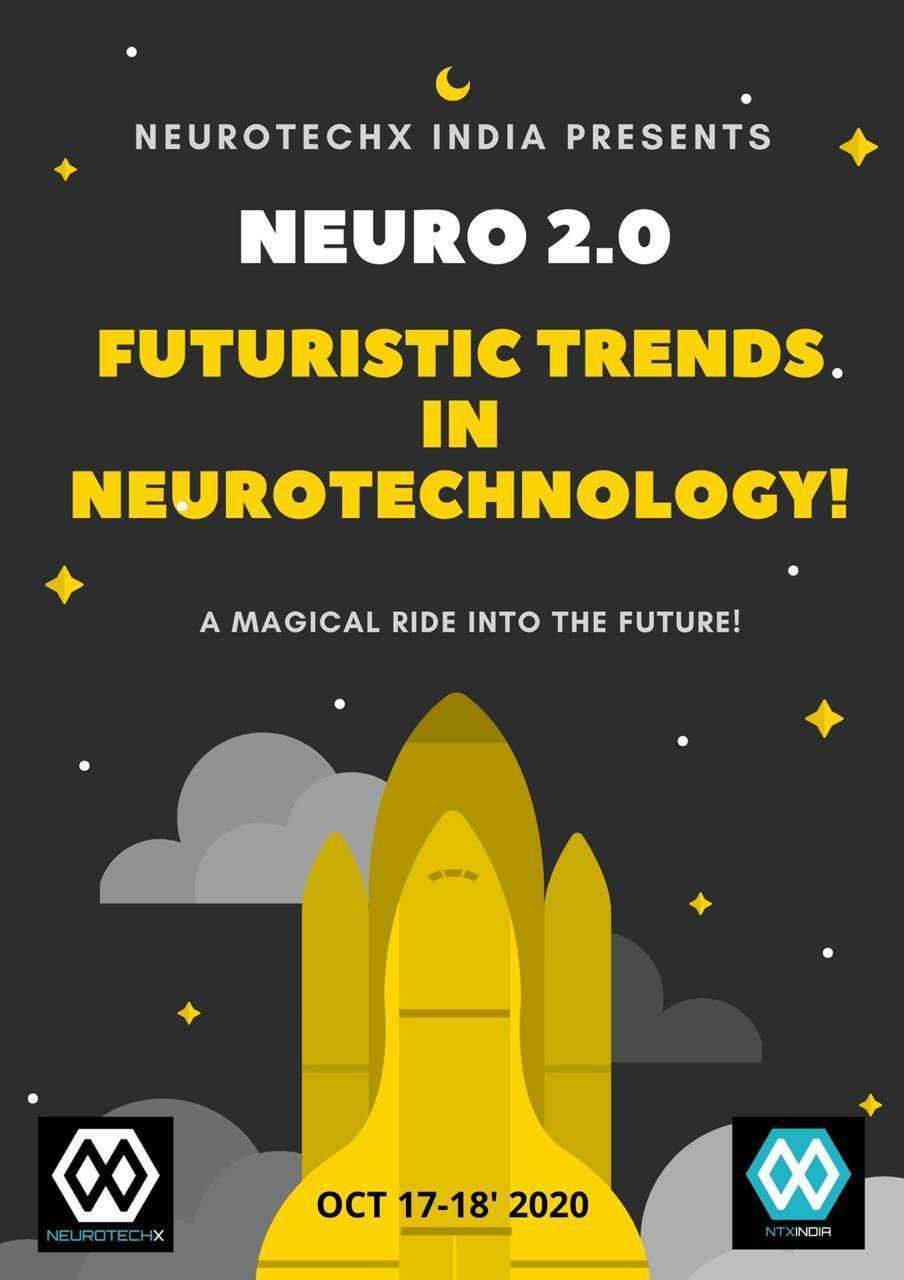
\includegraphics[width=\linewidth,height=46mm,keepaspectratio]{assets/chapters/india-neuro2-2020.jpg}
      \par\smallskip{\scriptsize Original NeuroTechX India event poster\par October 17--18, 2020\par}
  \end{columns}
  {\tiny\color{NTXMuted}Sources: \href{https://neurostars.org/t/neuro-2-0-futuristic-trends-in-neurotechnology/16962}{Neuro 2.0 announcement / poster}; \href{https://neurotechx.com/ntxbir2021/}{Buzz-in-Review 2021}; \href{https://eywaneuro.com/news}{Eywa Neuro: September 4, 2021 talk}\par}
  \note{[13:45--14:45] India is a country-wide community here, not a single city chapter. Neuro 2.0 ran online October 17--18, 2020. The original event artwork and announcement survive on Neurostars; speaker Pia Tikka's university research-group archive independently documents her participation alongside Isabella Pasqualini and David Eagleman on day two. The January 23, 2021 Buzz-in-Review program paired India and Australia. Eywa Neuro's own news archive records Kaustubh's invited September 4, 2021 NTX India talk on invasive BMI, microelectrodes, and India's role in bioMEMS manufacturing. These are documented milestones, not an asserted founding date or claims about attendance. The poster represents an online event, not evidence of an in-person gathering. The lesson is that a geographically distributed community can connect global expertise with local researchers and founders.}
\end{frame}


\begin{frame}{NeuroTechX Hacknights}
  \begin{columns}[T,onlytextwidth]
    \column{.52\textwidth}
      \NTXPoint{A recurring place to meet}{Newcomers and people already working on projects.}
      \NTXPoint{Across chapters}{San Francisco, Paris, and other local communities.}
      \NTXPoint{Work together}{Hardware, experiments, software, and help from peers.}
    \column{.43\textwidth}
      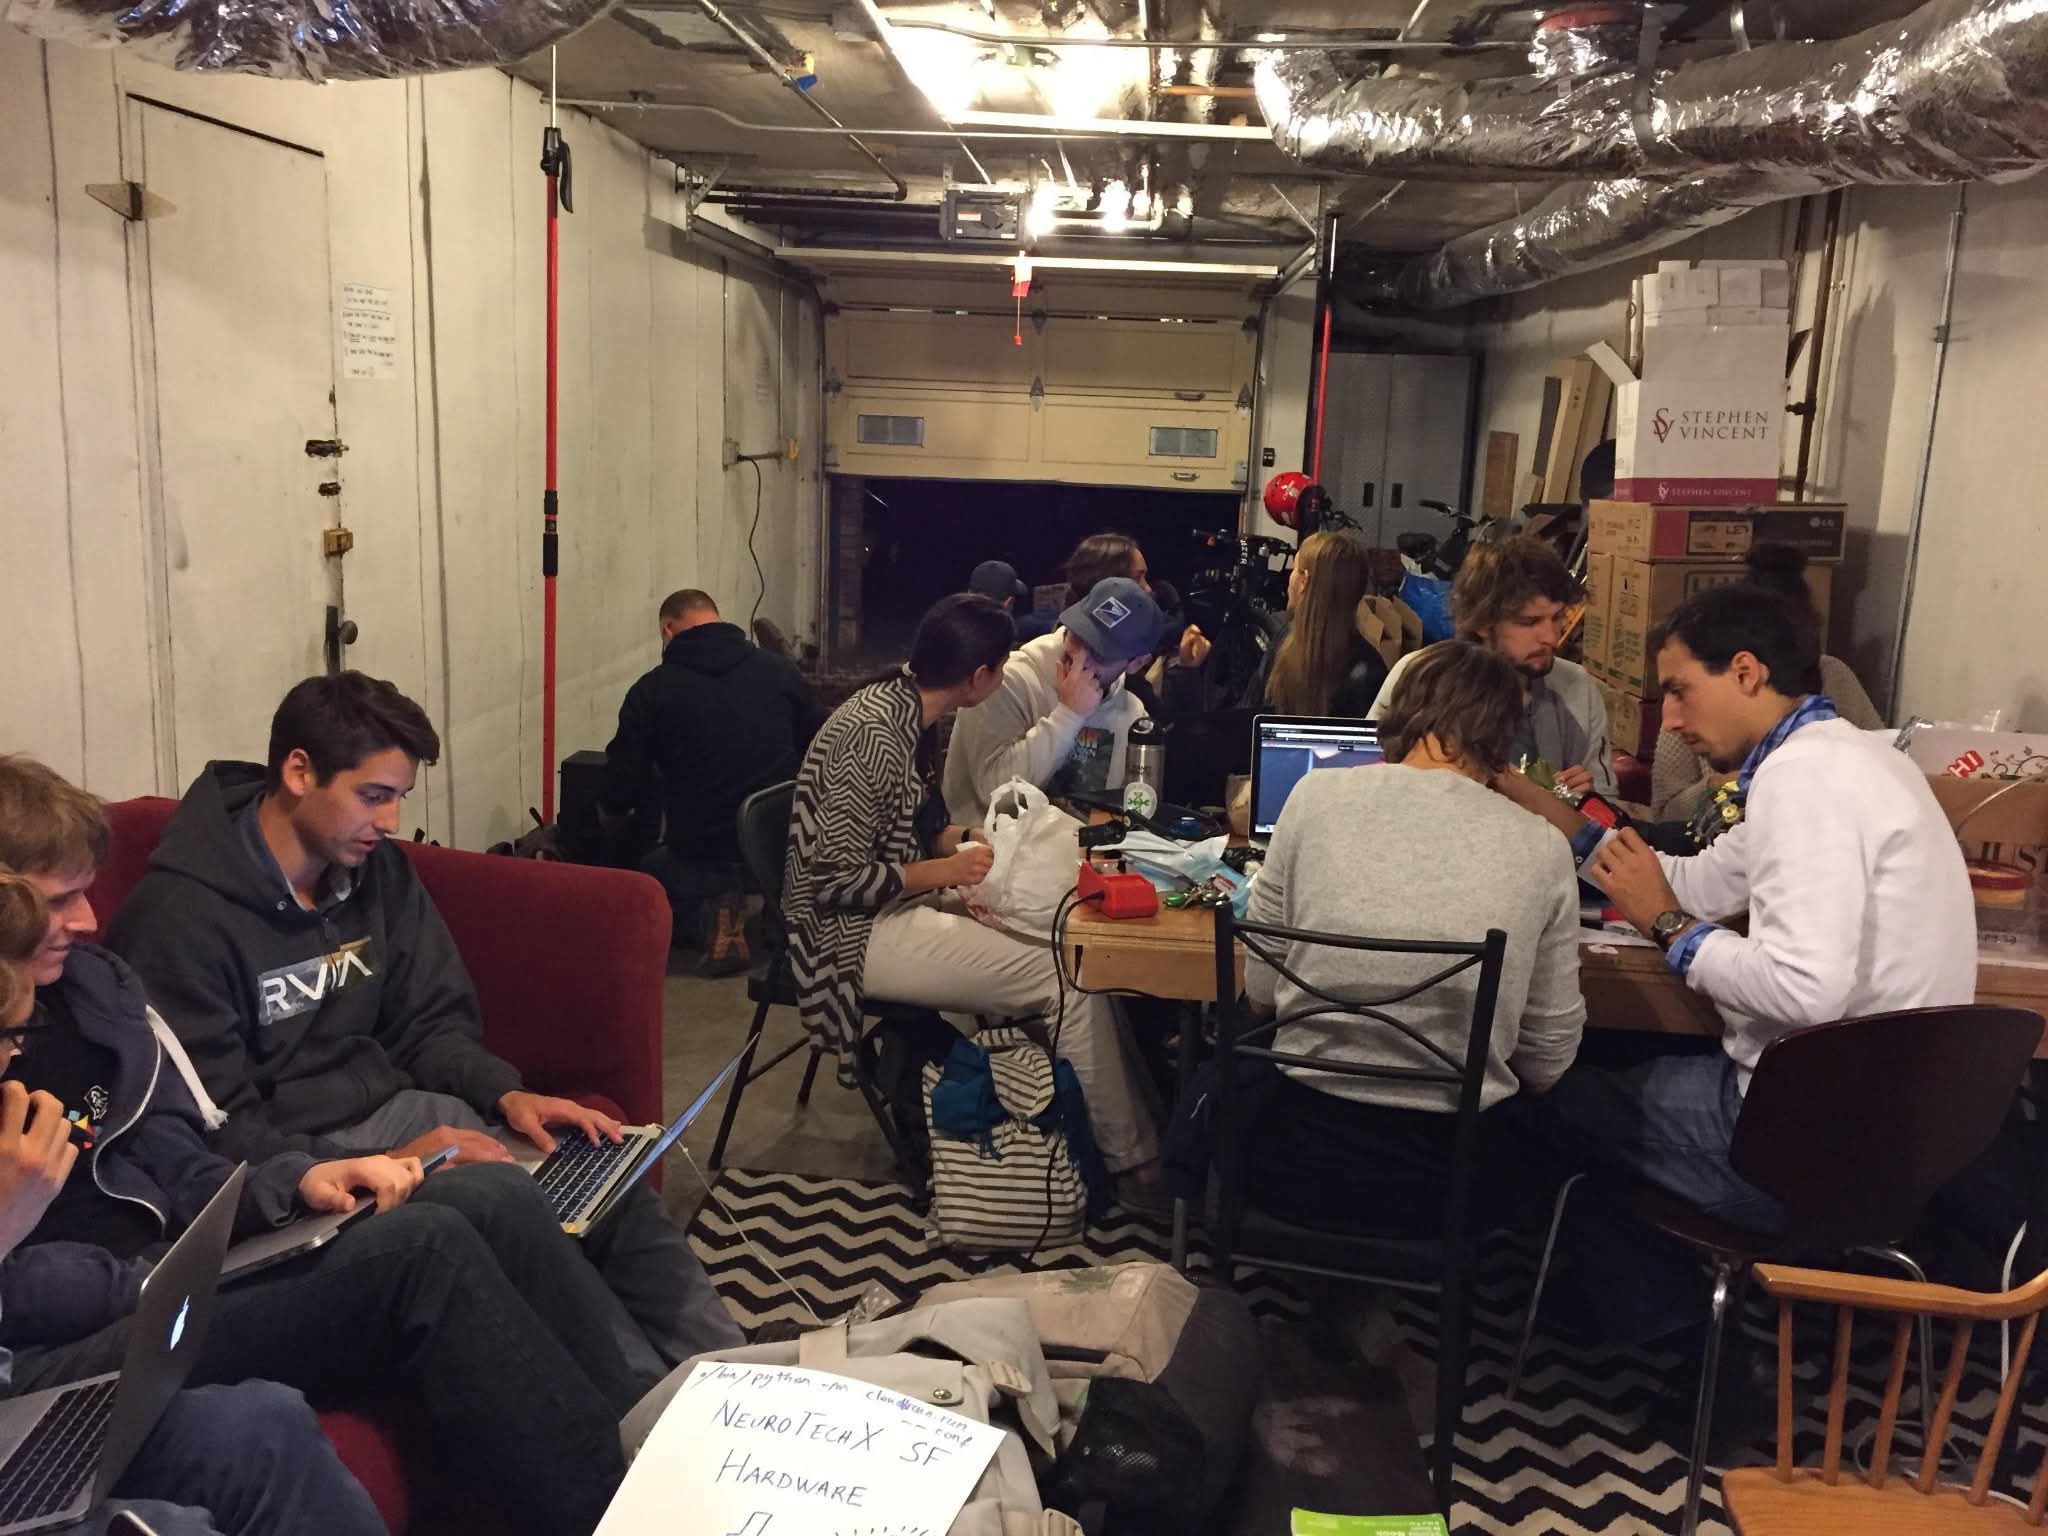
\includegraphics[width=\linewidth,height=47mm,keepaspectratio]{assets/chapters/san-francisco-original-hacknight.jpg}
      \par\smallskip{\scriptsize Original San Francisco Hacknights\par}
  \end{columns}
  {\tiny\color{NTXMuted}Photo supplied and identified by Morgan Hough\par}
  \note{[14:45--15:30] Hacknights are a NeuroTechX format, not only a San Francisco activity. This photograph shows the original SF hacknights, identified by Morgan and supplied as Image-1.jpg. Morgan also still cohosts the Paris Hacknights. Explain what a newcomer actually encounters: hardware, open science, software, and help from peers. Do not infer a date or identify individual participants from the photograph.}
\end{frame}

\begin{frame}{Buzz-in-Review: a shared annual chapter event}
  \begin{columns}[c,onlytextwidth]
    \column{.45\textwidth}
      \small
      \NTXPoint{The year in neurotechnology}{News and research for the general public.}
      \NTXPoint{Shared content, local conversations}{A common review for chapters to present and discuss.}
      \NTXPoint{A global format}{2021: 19 chapters across 10 online events.}
    \column{.51\textwidth}
      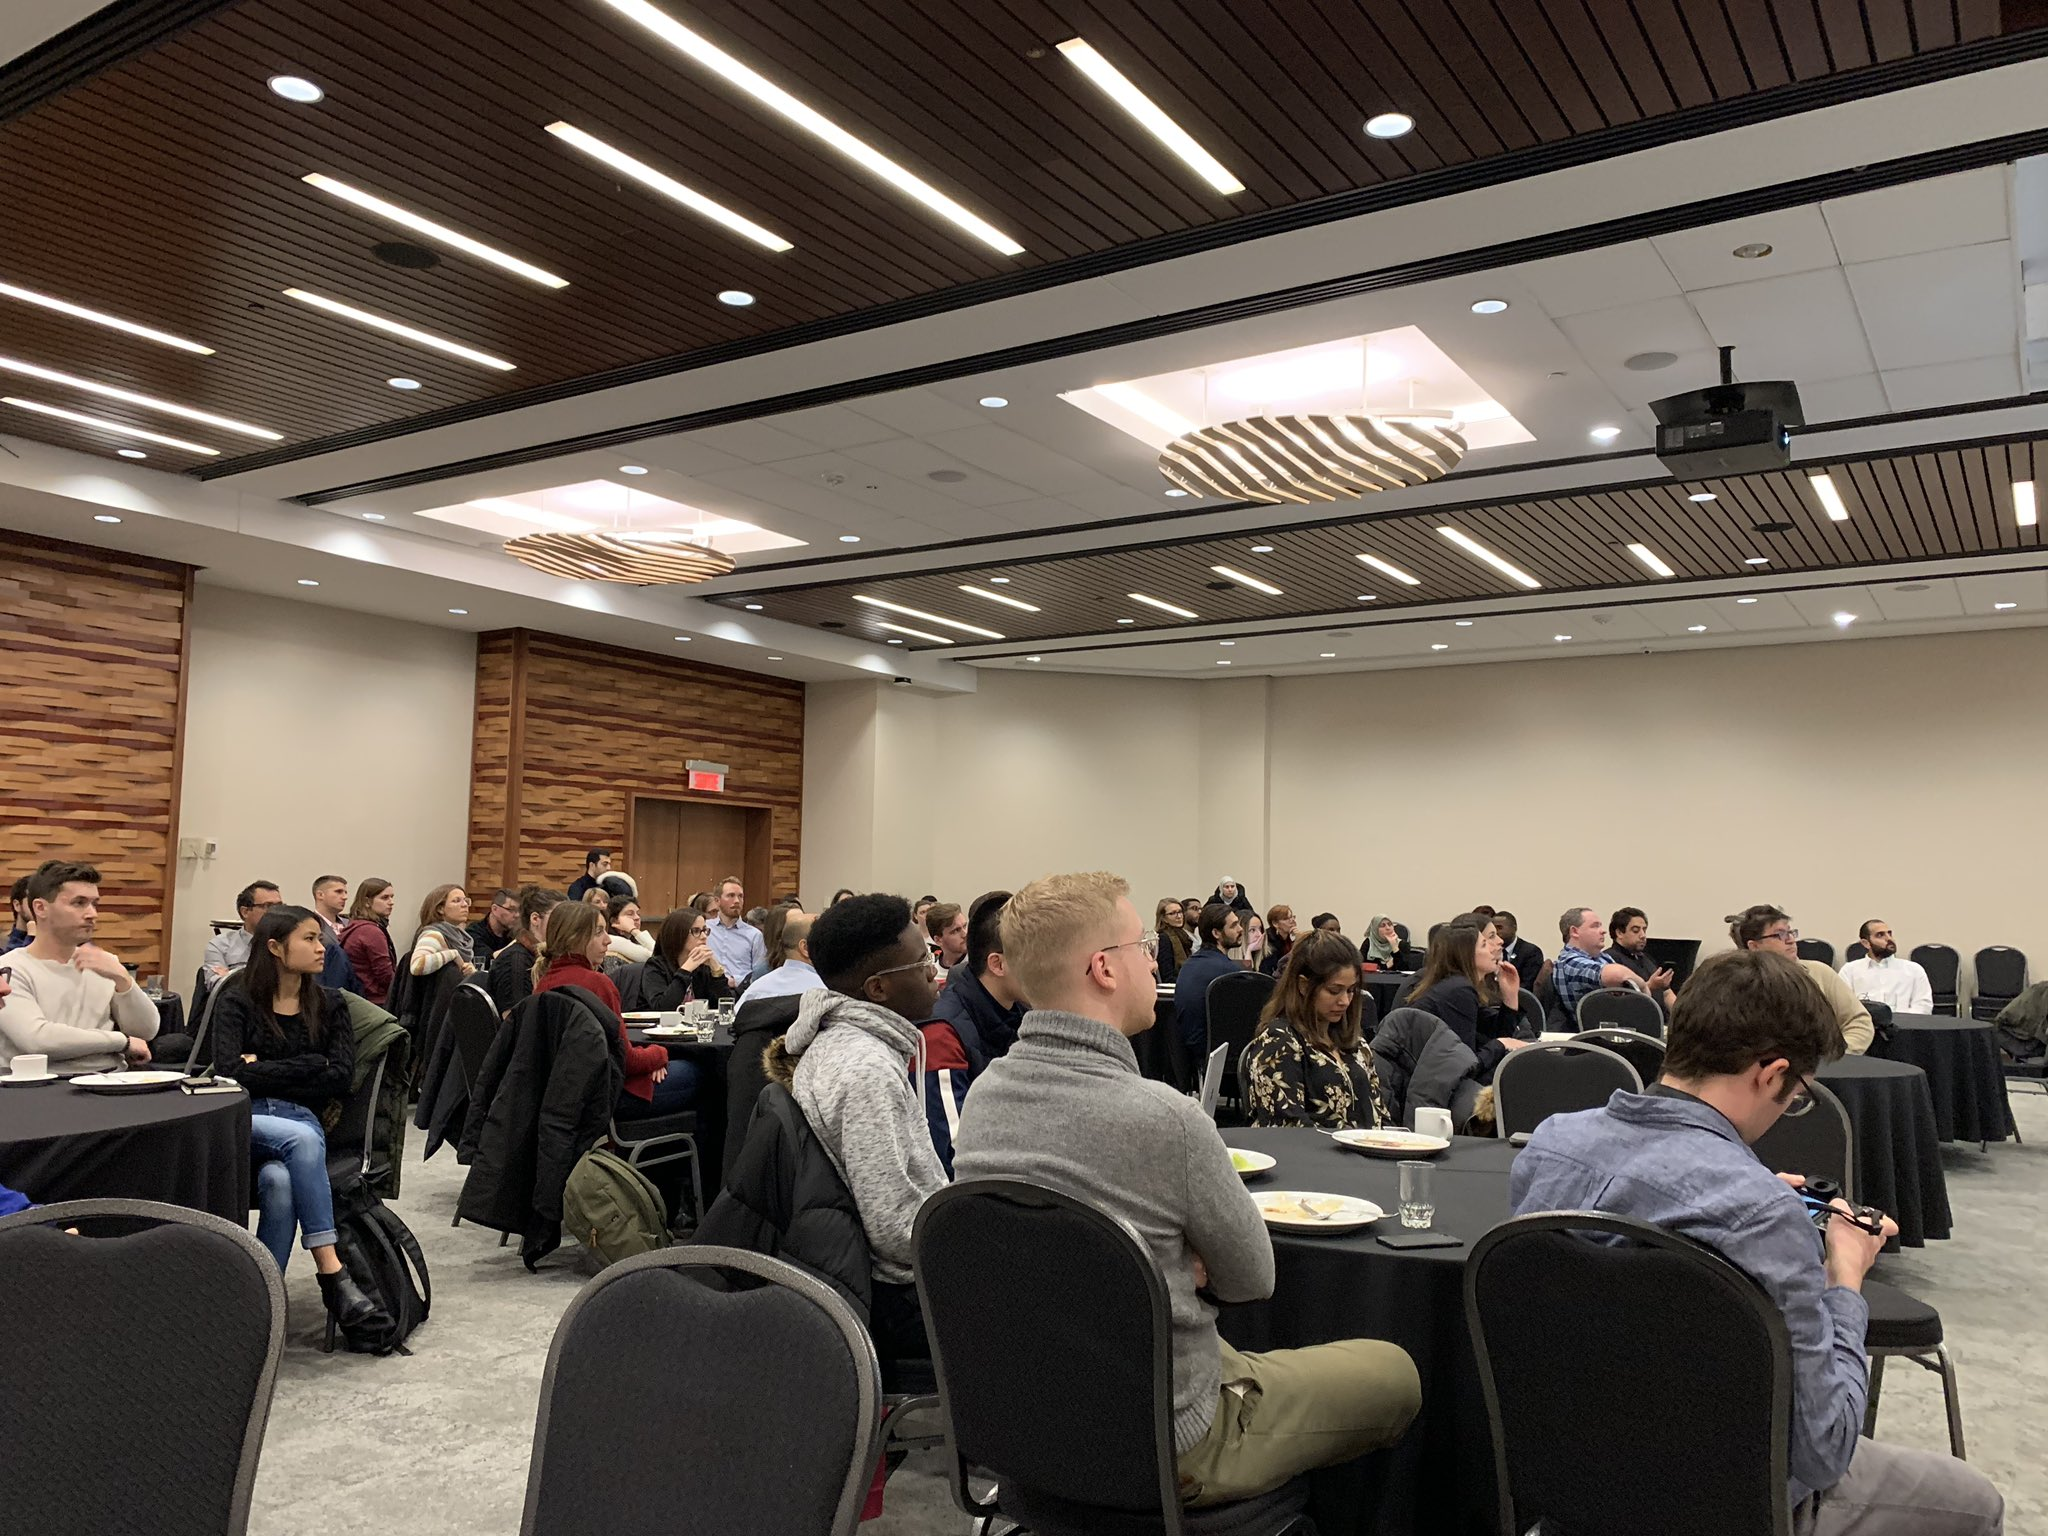
\includegraphics[width=\linewidth,height=45mm,keepaspectratio]{assets/chapters/montreal-buzz-in-review-2020.jpg}
      \par\smallskip{\scriptsize In person in Montr\'eal --- January 2020\par}
  \end{columns}
  {\tiny\color{NTXMuted}Sources: \href{https://neurotechx.com/ntxbir2021/}{Buzz in Review 2021}; photo: \href{https://twitter.com/NeuroTechMTL/status/1215643104847503363}{NeuroTechMTL}; \href{https://www.mcgill.ca/hbhl/channels/event/neurotech-buzz-review-2020-303563}{McGill / HBHL event listing}\par}
  \note{Photo: NeuroTechMTL's contemporaneous post identifies the in-person Montreal Buzz in Review 2020 event and HBHL's introduction. Retrieved via a public archive of the chapter's post; the original media URL was checked. McGill independently lists the January 9, 2020 event at New Residence Hall. The pictured event is distinct from the online 2021 program described in the text.}
  \note{[15:30--17:00] Morgan describes the annual event as providing city chapters with news and research for the general public. The 2021 event page lists 19 chapters and 10 online events; these are program figures, not audience counts. Explain how shared review material supports local public-facing conversations. Do not claim every chapter participates every year or that every event follows the same format.}
\end{frame}

\begin{frame}{NeuroTechX Content Laboratory}
  \begin{columns}[c,onlytextwidth]
    \column{.46\textwidth}
      \small
      \NTXPoint{Writers, editors, and designers}{Original articles and varied perspectives on neurotechnology.}
      \NTXPoint{Another way to contribute}{Explain the field, share a project story, or edit someone else's work.}
      \NTXPoint{A recent example}{The Future of Brain Medicine with Owen Muir\\Interview by Chay Carter, May 2026}
    \column{.50\textwidth}
      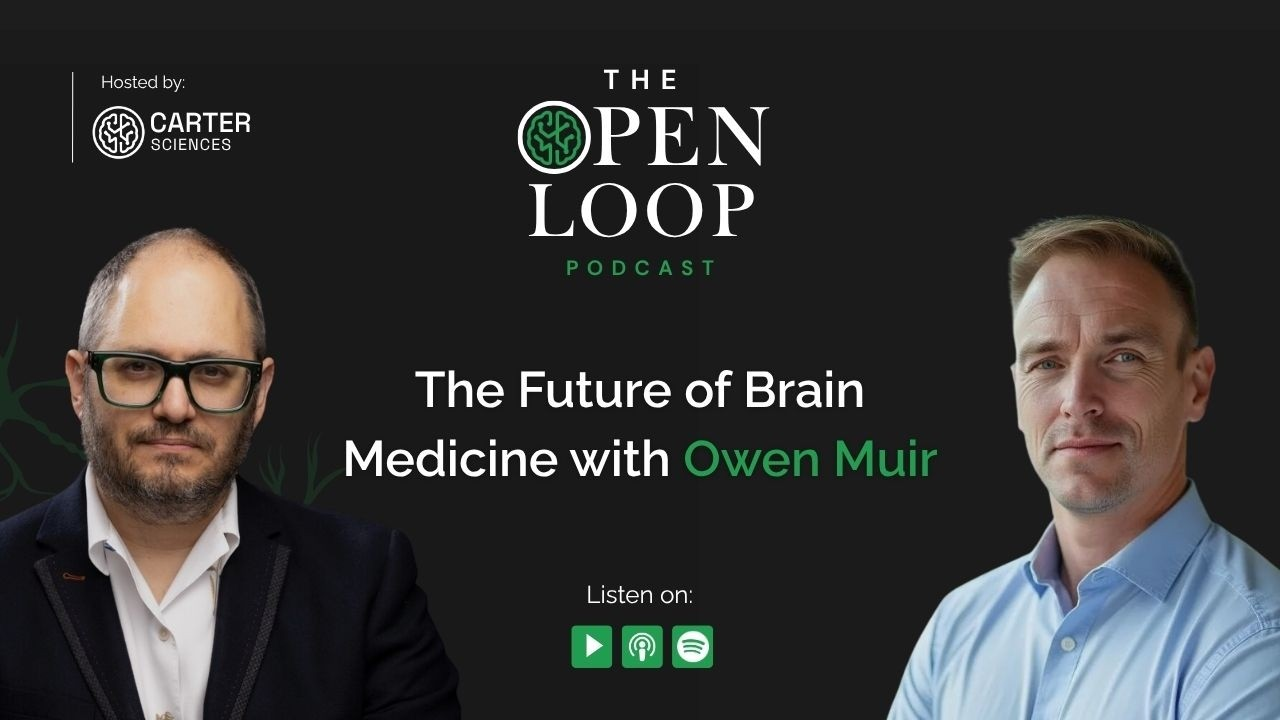
\includegraphics[width=\linewidth,height=40mm,keepaspectratio]{assets/history/content-lab-owen-interview.jpg}
      \par\smallskip{\scriptsize Original interview artwork: The Open Loop / Carter Sciences\par}
  \end{columns}
  {\tiny\color{NTXMuted}\href{https://medium.com/neurotechx/the-future-of-brain-medicine-with-owen-muir-a02360f770d5}{Read the Content Lab article}; \href{https://medium.com/neurotechx}{medium.com/neurotechx}; \href{https://www.youtube.com/watch?v=1ooyWf79Vyo}{original interview / image}\par}
  \note{[17:00--18:30] The publication brings together writers, editors, and designers. Community participation also includes communicating and explaining the work. The example is Chay Carter's interview with Owen Muir, published by the Content Lab on May 18, 2026. Medium blocked direct image retrieval and browser capture, so the visual is artwork from the original Open Loop interview, not a screenshot of Medium. Carter's own public post links the Medium version, and Muir's May 14 post embeds the original video. Credit The Open Loop / Carter Sciences. This illustrates an editorial contribution; it does not endorse clinical claims in the interview or imply the independent podcast is owned by NeuroTechX.}
\end{frame}

\begin{frame}{The NeuroTechX newsletter: a long-running community resource}
  \begin{columns}[c,onlytextwidth]
    \column{.46\textwidth}
      \small
      \NTXPoint{An archive reaching back to 2015}{November 2015: NeuroTechX Digest \#1.}
      \NTXPoint{Keeping the community connected}{Research, industry developments, projects, events, and opportunities.}
      \NTXPoint{A record of the field as it develops}{\href{https://neurotechx.org/newsletter}{neurotechx.org/newsletter}}
    \column{.50\textwidth}
      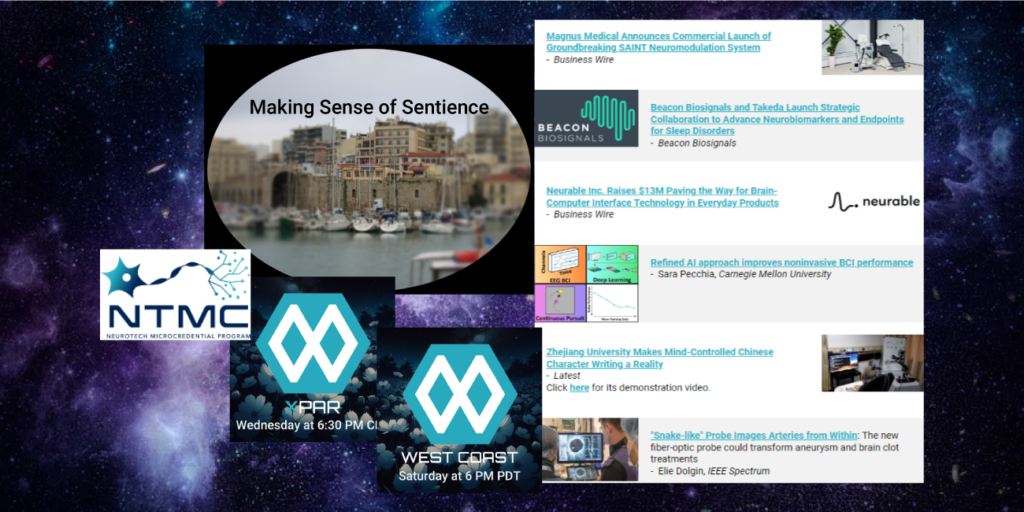
\includegraphics[width=\linewidth,height=40mm,keepaspectratio]{assets/history/ntx-newsletter-may2024.png}
      \par\smallskip{\scriptsize May 2024 newsletter --- official archive artwork\newline Image: NeuroTechX\par}
  \end{columns}
  \NTXSource{https://neurotechx.org/newsletter}{NeuroTechX newsletter archive; earliest listed edition: November 2015}
  \note{The image is NeuroTechX's May 2024 newsletter promotional collage from https://neurotechx.com/stay-tuned/, not a new screenshot or current issue. Original image filename: 20240522\_Newsletter-1024x512.png. It demonstrates the mix of community events, educational opportunities, research, and industry updates; dated headlines are not presented as current news.}
  \note{[18:30--20:00] Morgan emphasizes the newsletter's longevity and its role in keeping the community informed. The public archive lists Digest 1 in November 2015, selected earlier editions, and monthly editions in later years. It does not establish uninterrupted publication or a field-wide longevity ranking. Neurotech Reports dates Neurotech Business Report to 2001, so it clearly predates NTX. Use the documented start of the archive rather than claim first or second longest-running. Discuss the editorial work of maintaining a shared resource across changing projects and cohorts.}
\end{frame}

\NTXDivider{Open Source Software Delivers}
\begin{frame}{EEG-ExPy: roots in muse-lsl and eeg-notebooks}
  \begin{columns}[T,onlytextwidth]
    \column{.66\textwidth}
      \NTXPoint{muse-lsl: access to the signal}{Alexandre Barachant's groundwork for streaming Muse EEG through Lab Streaming Layer.}
      \NTXPoint{eeg-notebooks: build the experiment}{Community-developed protocols combining recording, stimulus presentation, and analysis.}
      \NTXPoint{EEG-ExPy: carry the work forward}{John Griffiths and contributors; PsychoPy for experiments, MNE for analysis.}
    \column{.28\textwidth}
      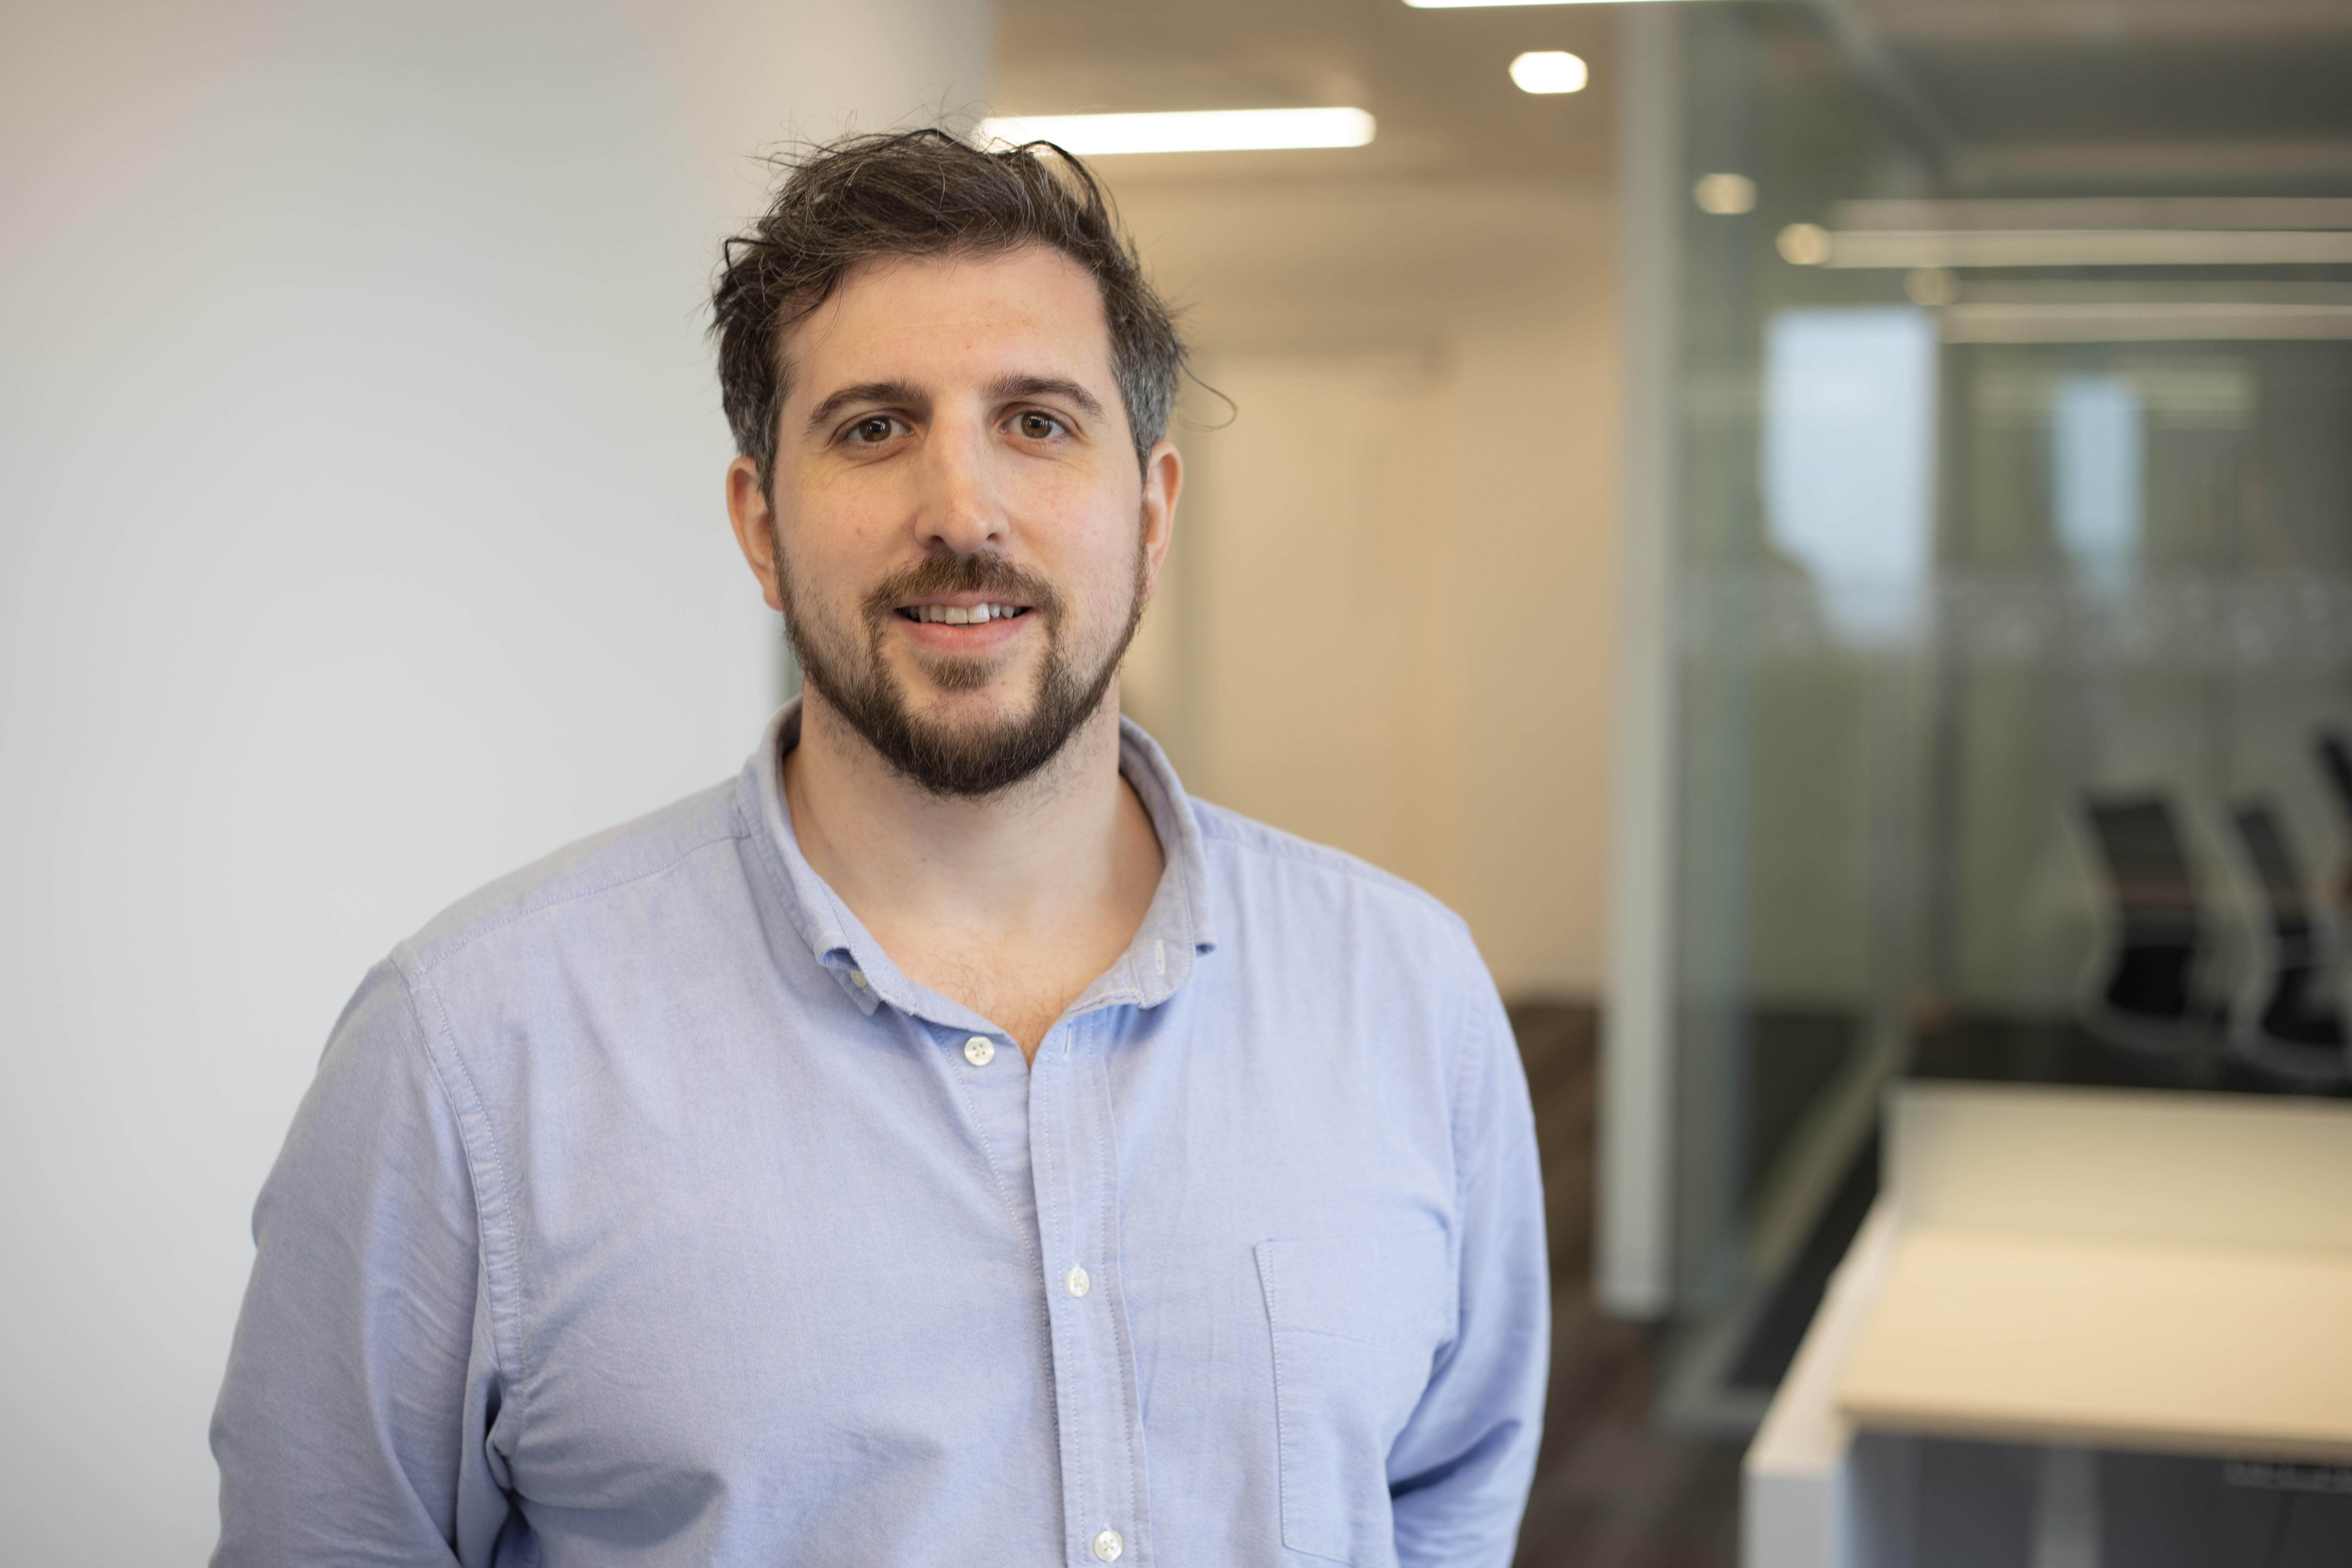
\includegraphics[width=\linewidth]{assets/people/john-griffiths.jpg}
      \par\smallskip{\small John Griffiths\par}
      \medskip{\scriptsize \href{https://www.crowdcast.io/e/brainhack-ontario/7}{Brainhack Ontario 2020\\introductory talk}\par}
  \end{columns}
  {\tiny\color{NTXMuted}Sources: \href{https://github.com/NeuroTechX/EEG-ExPy}{EEG-ExPy history and credits}; \href{https://www.grifflab.com/code_and_software/eeg-notebooks/}{Griffiths, 2019}; portrait: CAMH\par}
  \note{[20:00--21:15] The README credits Alexandre Barachant with the initial idea and much of the groundwork, including muse-lsl, and identifies John Griffiths as lead developer alongside many contributors. eeg-notebooks was later renamed EEG-ExPy; muse-lsl is a foundational dependency, not an earlier name for the same project. John's January 4, 2019 lab account describes the NTX/InterAxon connection, Brainhack experimentation, and educational use through NeuroBRITE and BrainWaves. Archived v0.2 documentation identifies his Brainhack Ontario 2020 introductory presentation and links the Crowdcast recording. The recording could not be retrieved during this edit; no quotation, screenshot, or claim about its specific contents is made. The original PsychoPy illustration has been removed from this slide, but its asset remains in the repository.}
\end{frame}

\begin{frame}{BrainFlow: shared access to more devices}
  \begin{columns}[c,onlytextwidth]
    \column{.53\textwidth}
      \small
  \NTXPoint{A common biosignal interface}{An open-source library for acquiring and processing EEG, EMG, ECG, and other sensor data.}
  \NTXPoint{Broader hardware access for EEG-ExPy}{Its device layer includes BrainFlow routes for OpenBCI, FreeEEG32, Muse, and other devices.}
  \NTXPoint{Build on each other's work}{EEG-ExPy credits Andrey Parfenov and BrainFlow for expanding device support.}
    \column{.43\textwidth}
      \centering
      {\small OpenBCI \quad FreeEEG32 \quad Muse\par}
      {\Large $\downarrow$\par}
      \fbox{\parbox{.88\linewidth}{\centering\textbf{BrainFlow}\par\small One acquisition API}}
      \par{\Large $\downarrow$\par}
      {\small Experiments \quad Analysis\newline Visualization\par}
      \par\smallskip{\scriptsize Conceptual device-to-software interface\par}
  \end{columns}
  {\scriptsize muse-lsl and BrainFlow coexist in EEG-ExPy's device layer.\par}
  \medskip
  {\tiny\color{NTXMuted}Sources: \href{https://brainflow.readthedocs.io/en/stable/}{BrainFlow documentation}; \href{https://github.com/NeuroTechX/EEG-ExPy/blob/master/eegnb/devices/eeg.py}{EEG-ExPy device layer}; \href{https://github.com/NeuroTechX/EEG-ExPy}{project acknowledgements}\par}
  \note{[21:15--22:45] BrainFlow is a separate open-source project, not an NTX-owned library. The EEG-ExPy README credits Andrey Parfenov and BrainFlow with expanding supported devices. The eegnb/devices/eeg.py module routes devices through BrainFlow or muse-lsl and includes OpenBCI variants, FreeEEG32, Muse variants, and a synthetic device. This is evidence of implemented integration, not a fresh end-to-end hardware compatibility test. A July 20, 2021 discussion records John considering BrainFlow's Muse support and native Bluetooth requirements; it does not date the initial integration or establish a completed migration then. Do not imply every BrainFlow-supported board is automatically supported by EEG-ExPy, that all boards perform equivalently, or that muse-lsl was entirely replaced. The community lesson is shared infrastructure enabling reuse across hardware.}
\end{frame}



\begin{frame}{Open-source hardware: making participation accessible}
  \begin{columns}[c,onlytextwidth]
    \column{.54\textwidth}
      \small
  \NTXPoint{Beyond low-cost EEG boards}{Access to instruments people can study, adapt, and improve.}
  \NTXPoint{OpenEIT / Spectra --- Jean Rintoul}{Electrical impedance tomography: shared hardware, firmware, and reconstruction tools.}
  \NTXPoint{un0rick --- Luc Jonveaux}{Low-cost, open ultrasound pulse-echo hardware for learning and research.}
      {\scriptsize Jean and Luc both presented at CogLab / NeuroTechX Paris Hacknights.\par}
    \column{.42\textwidth}
      \centering
      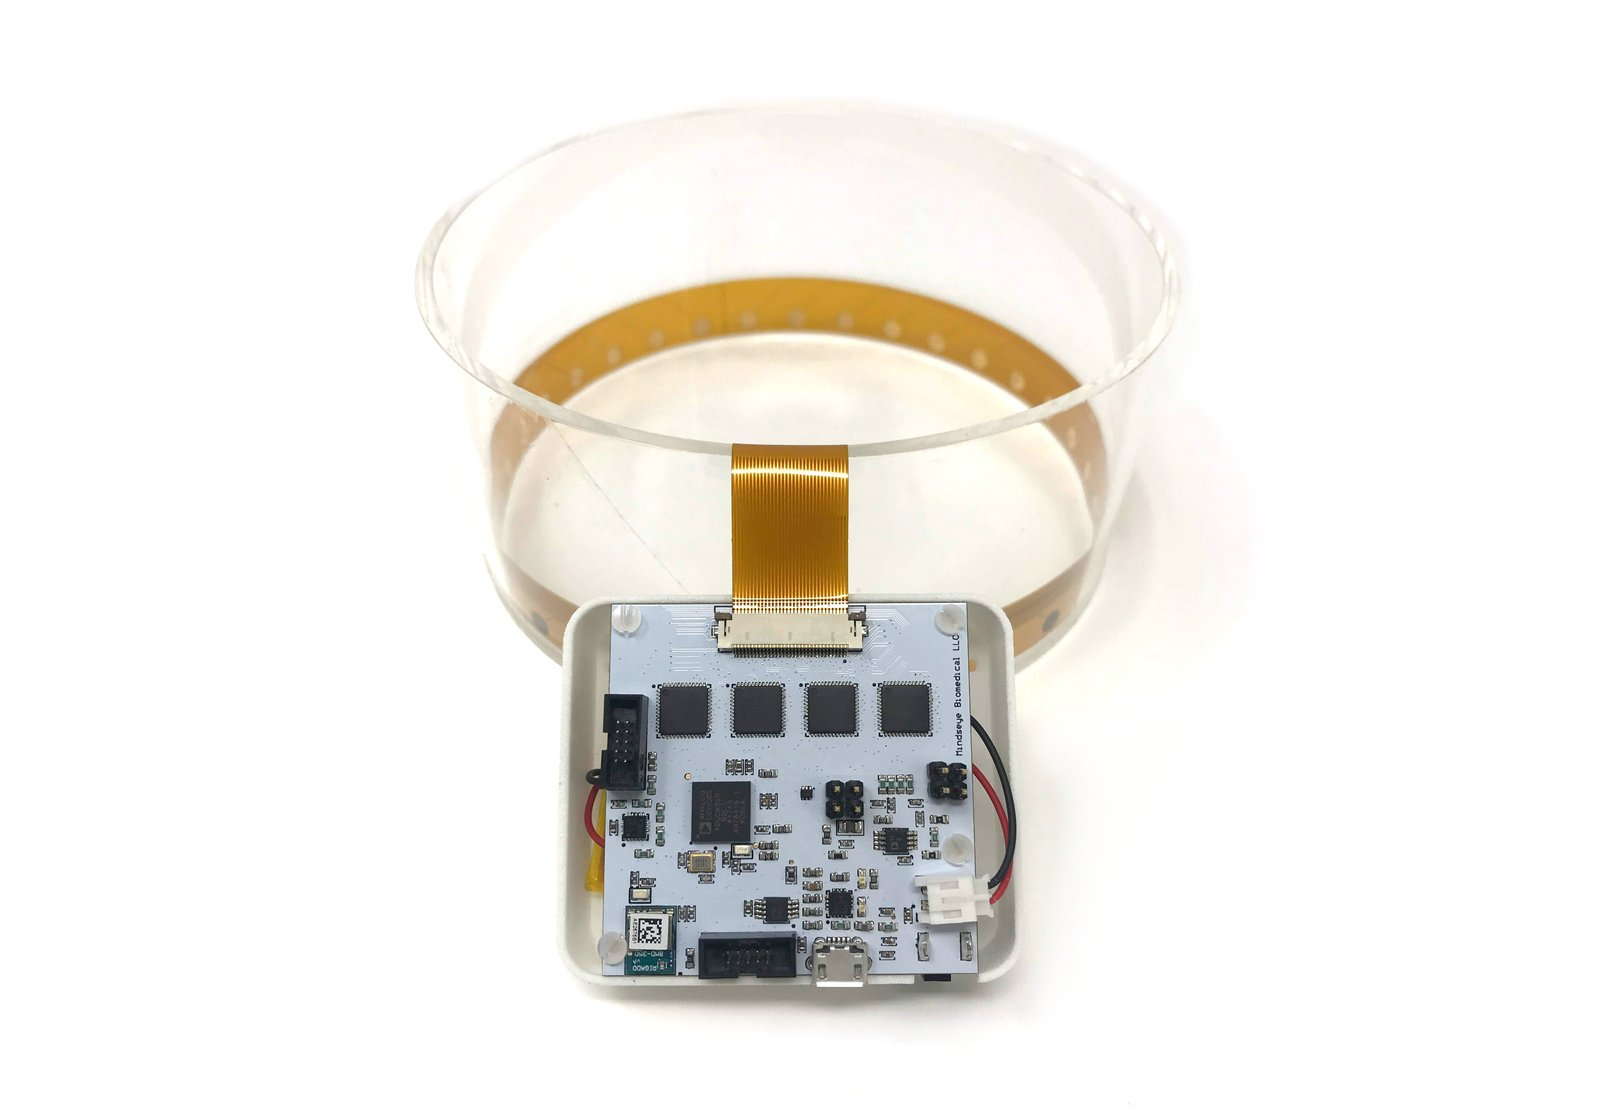
\includegraphics[width=\linewidth,height=23mm,keepaspectratio]{assets/history/spectra-kit.jpg}\par
      {\tiny Spectra --- Mindseye Biomedical / Crowd Supply\par}\smallskip
      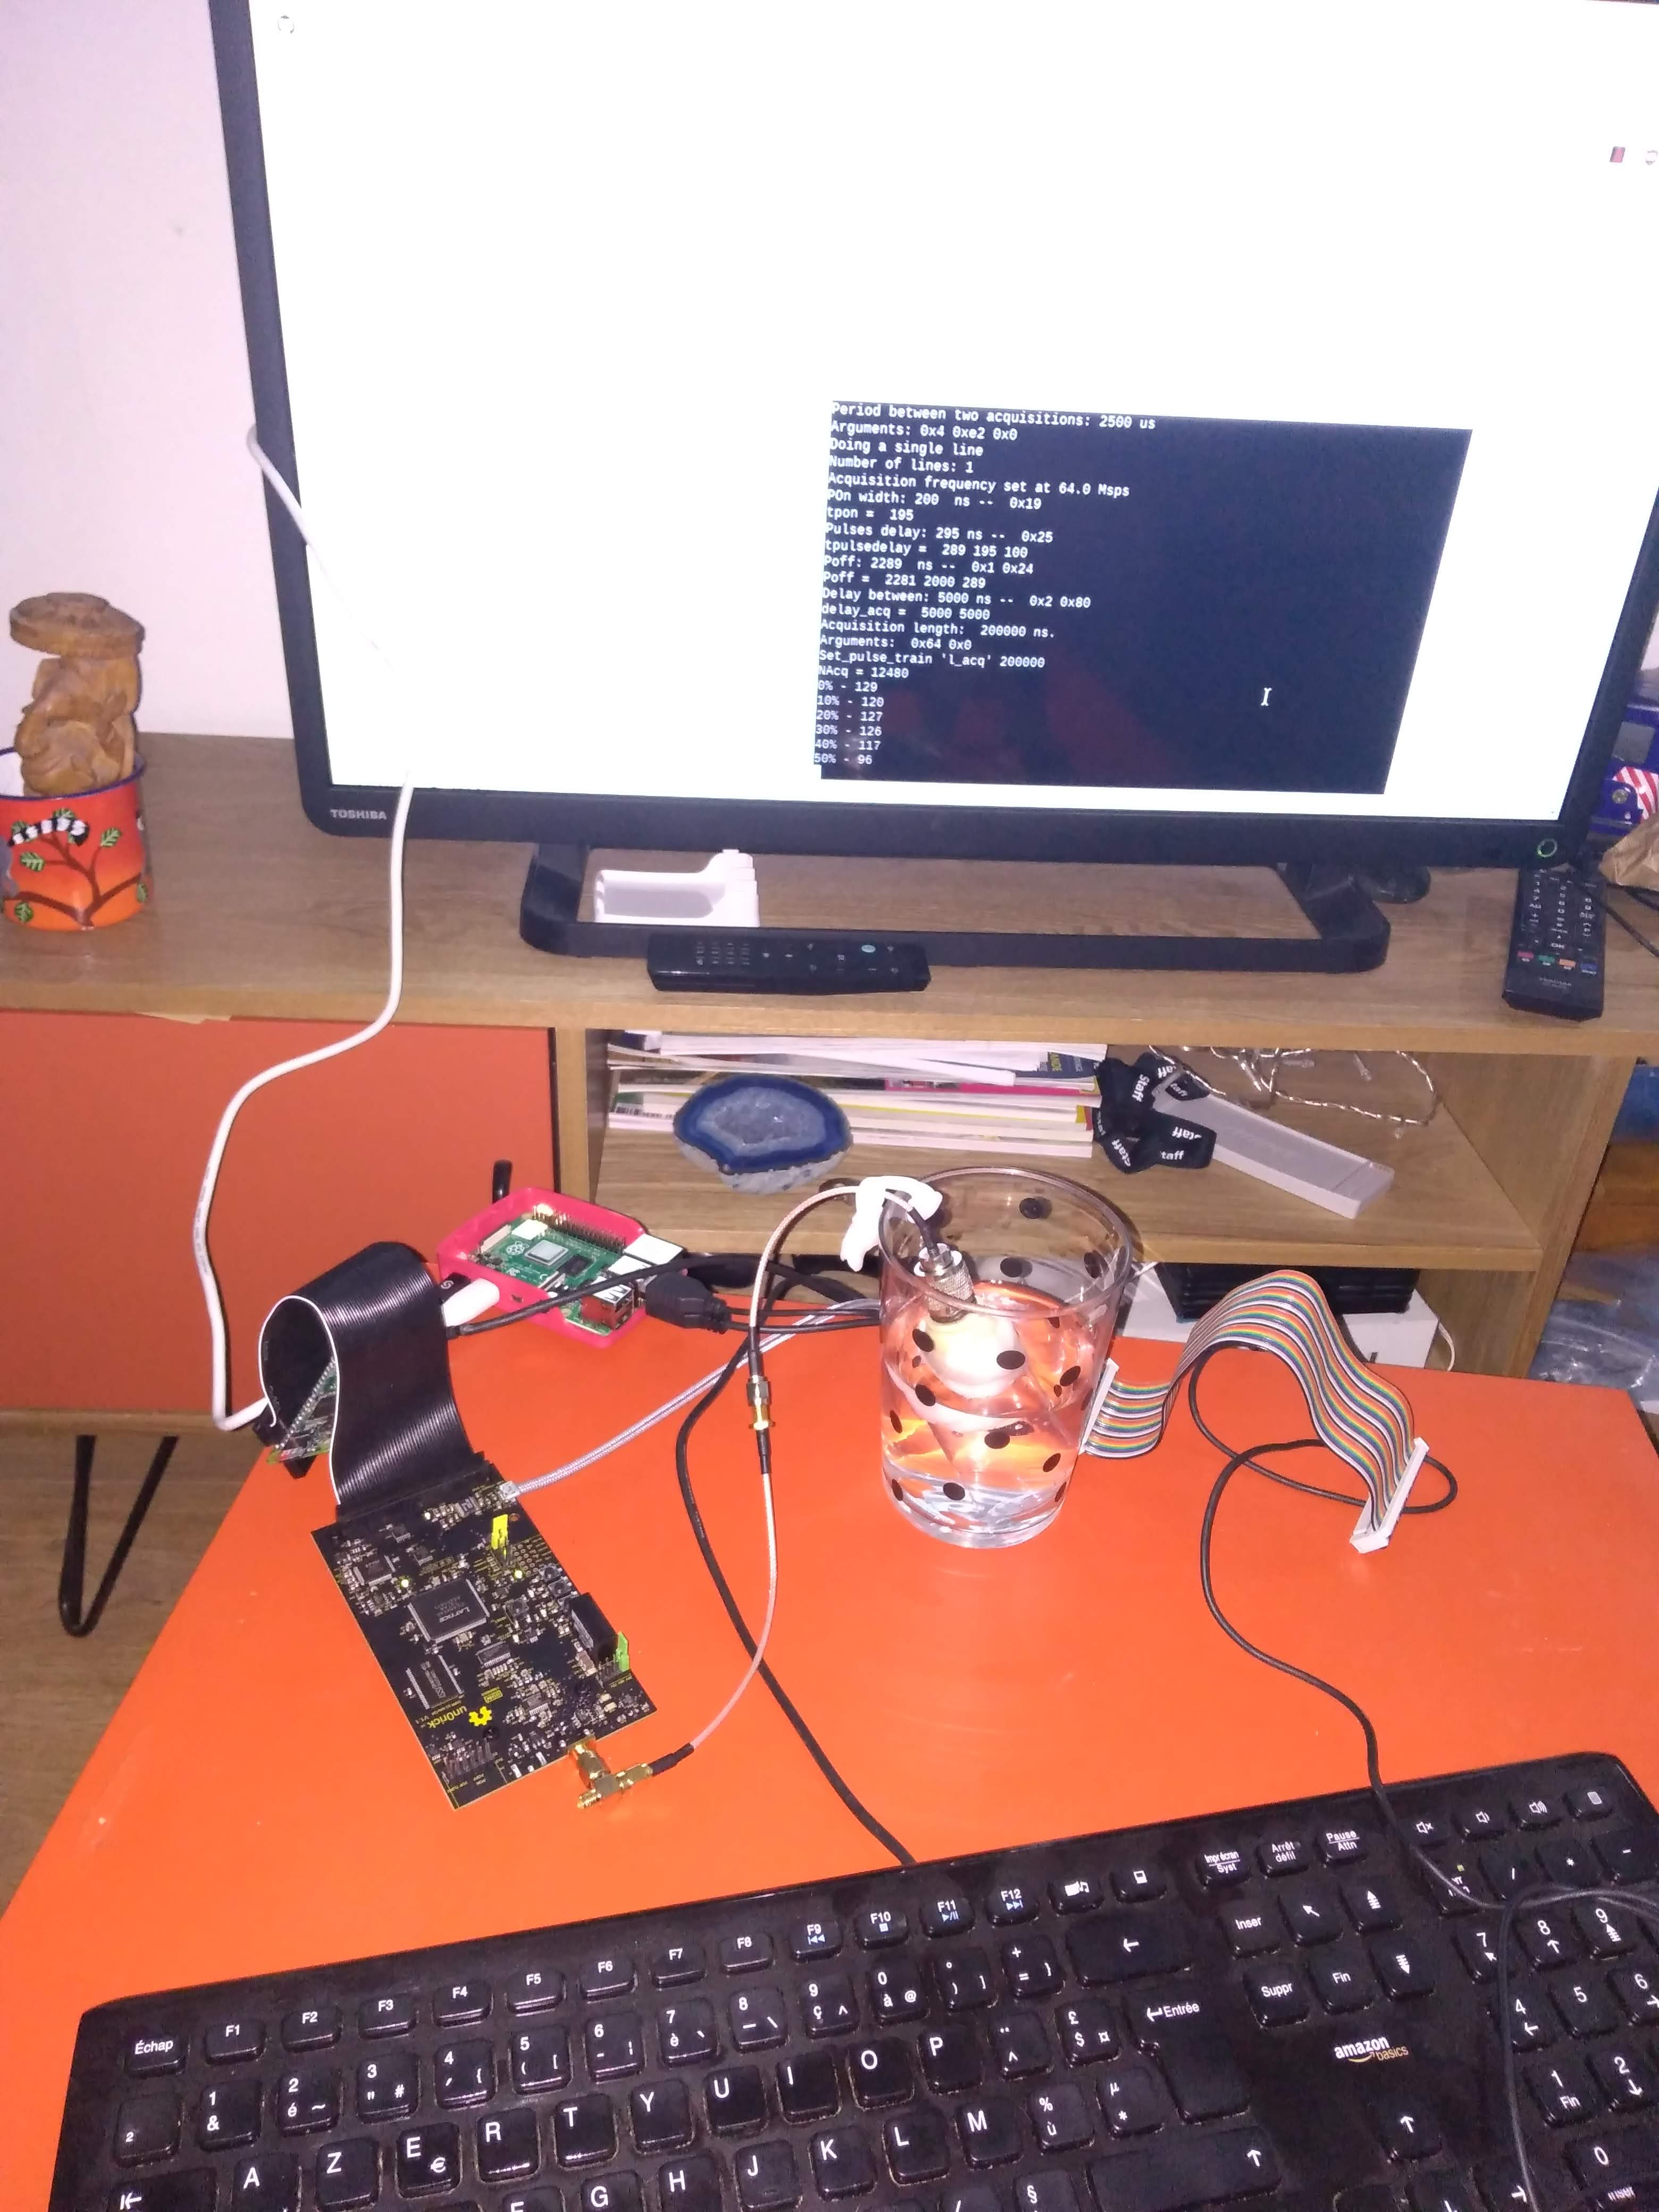
\includegraphics[width=\linewidth,height=24mm,keepaspectratio]{assets/history/un0rick-bench.jpg}\par
      {\tiny un0rick bench test --- \href{https://un0rick.cc/un0rick}{Luc Jonveaux / kelu124}\par}
  \end{columns}
  \medskip
  {\tiny\color{NTXMuted}Sources: \href{https://www.crowdsupply.com/mindseye-biomedical/spectra}{Rintoul / Mindseye: Spectra}; \href{https://doi.org/10.5334/joh.28}{Jonveaux, Schloh, Meng, Arija \& Rintoul, 2022}; \href{https://coglab.fr/activites/hacknight/}{CogLab Hacknights}\par}
  \note{[22:45--24:15] Morgan identifies support for low-cost EEG boards, OpenEIT, and ultrasound as part of NTX's contribution. CogLab's archive specifically lists Jean Rintoul presenting Spectra at HackNight 150 (June 8) and Luc Jonveaux presenting un0rick at HackNight 148 (May 18). This verifies community exposure and discussion, not funding or NTX ownership. Jean's OpenEIT documentation and Mindseye's December 5, 2019 Spectra update emphasize tutorials and lowering the entry barrier. She coauthored the 2022 Journal of Open Hardware review with Jonveaux, Schloh, Meng, and Arija. The lesson is that affordability needs documentation and people who can help newcomers. These are research and educational examples, not claims of clinical readiness, safe self-experimentation, or diagnostic equivalence. OpenEIT firmware includes noncommercial licensing restrictions: do not imply unrestricted commercial reuse. un0rick is the historical FPGA board; the project's current site also describes its newer pic0rick design.}
\end{frame}

\begin{frame}{OpenEIT: sharing the work with wider communities}
  \begin{columns}[T,onlytextwidth]
    \column{.49\textwidth}
      \NTXPoint{Jean Rintoul at 34C3}{Low-cost biomedical imaging through electrical impedance tomography.}
      \NTXPoint{OpenEIT at LIBRE Hub}{Sharing the principles, project history, and directions for accessible imaging.}
      {\small Open tools need places where people can encounter them and learn.\par}
    \column{.46\textwidth}
      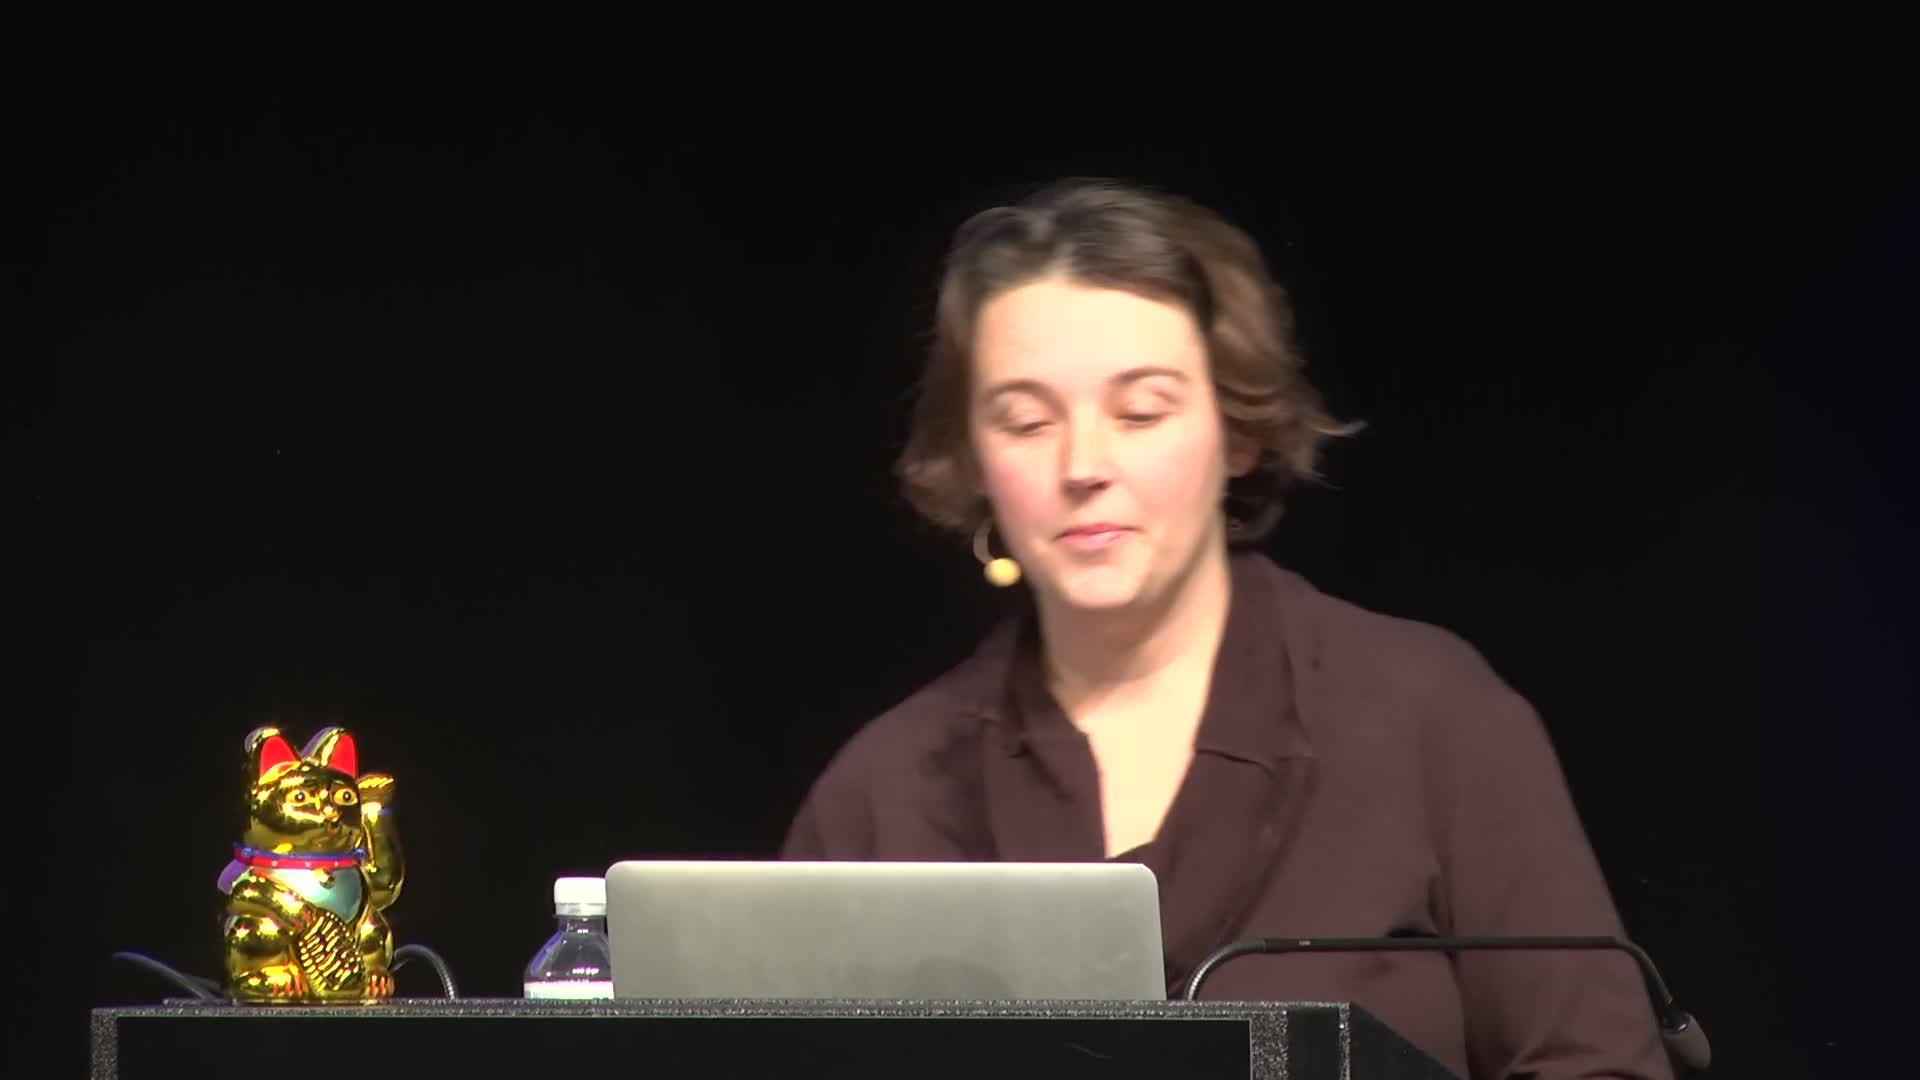
\includegraphics[width=\linewidth]{assets/people/jean-rintoul-34c3-speaking.jpg}
      \par\smallskip{\scriptsize Jean Rintoul speaking at the\\34th Chaos Communication Congress\\27 December 2017\par}
  \end{columns}
  \medskip
  {\tiny\color{NTXMuted}Frame: \href{https://media.ccc.de/v/34c3-8948-low_cost_non-invasive_biomedical_imaging}{CCC recording, 01:20}; \href{https://librehub.github.io/2025/12/02/jean-rintoul.html}{LIBRE Hub OpenEIT seminar}\par}
  \note{[24:15--25:45] The image is a frame extracted at 01:20 from Jean's official 34C3 recording, Low Cost Non-Invasive Biomedical Imaging: An Open Electrical Impedance Tomography Project, dated December 27, 2017. This is an actual speaking image, not a generated portrait. LIBRE Hub separately lists her OpenEIT seminar and its scope. Its homepage advertises January 15, 2026 but the detail page says January 15, 2025 despite a December 2025 URL; omit the year until clarified. No accessible LIBRE Hub recording or speaking photograph was found, so this image is labeled only as Congress. These are external dissemination venues, not events claimed as organized by NTX.}
\end{frame}

\begin{frame}{Low-cost EEG: more ways to start building}
  \begin{columns}[c,onlytextwidth]
    \column{.57\textwidth}
      \small
      \NTXPoint{icibici --- Colin Rowat and collaborators}{Single-channel EEG via an audio connection.\newline Credits NeuroTechX and its Slack community.}
      \NTXPoint{FreeEEG32}{Open-source, 32-channel acquisition.\newline Custom nets developed by Bernard Markus.}
      \NTXPoint{Neurogate / OctaFlow}{EEG, EMG, and ECG acquisition;\newline connections to LSL and Timeflux.}
    \column{.39\textwidth}
      \centering
      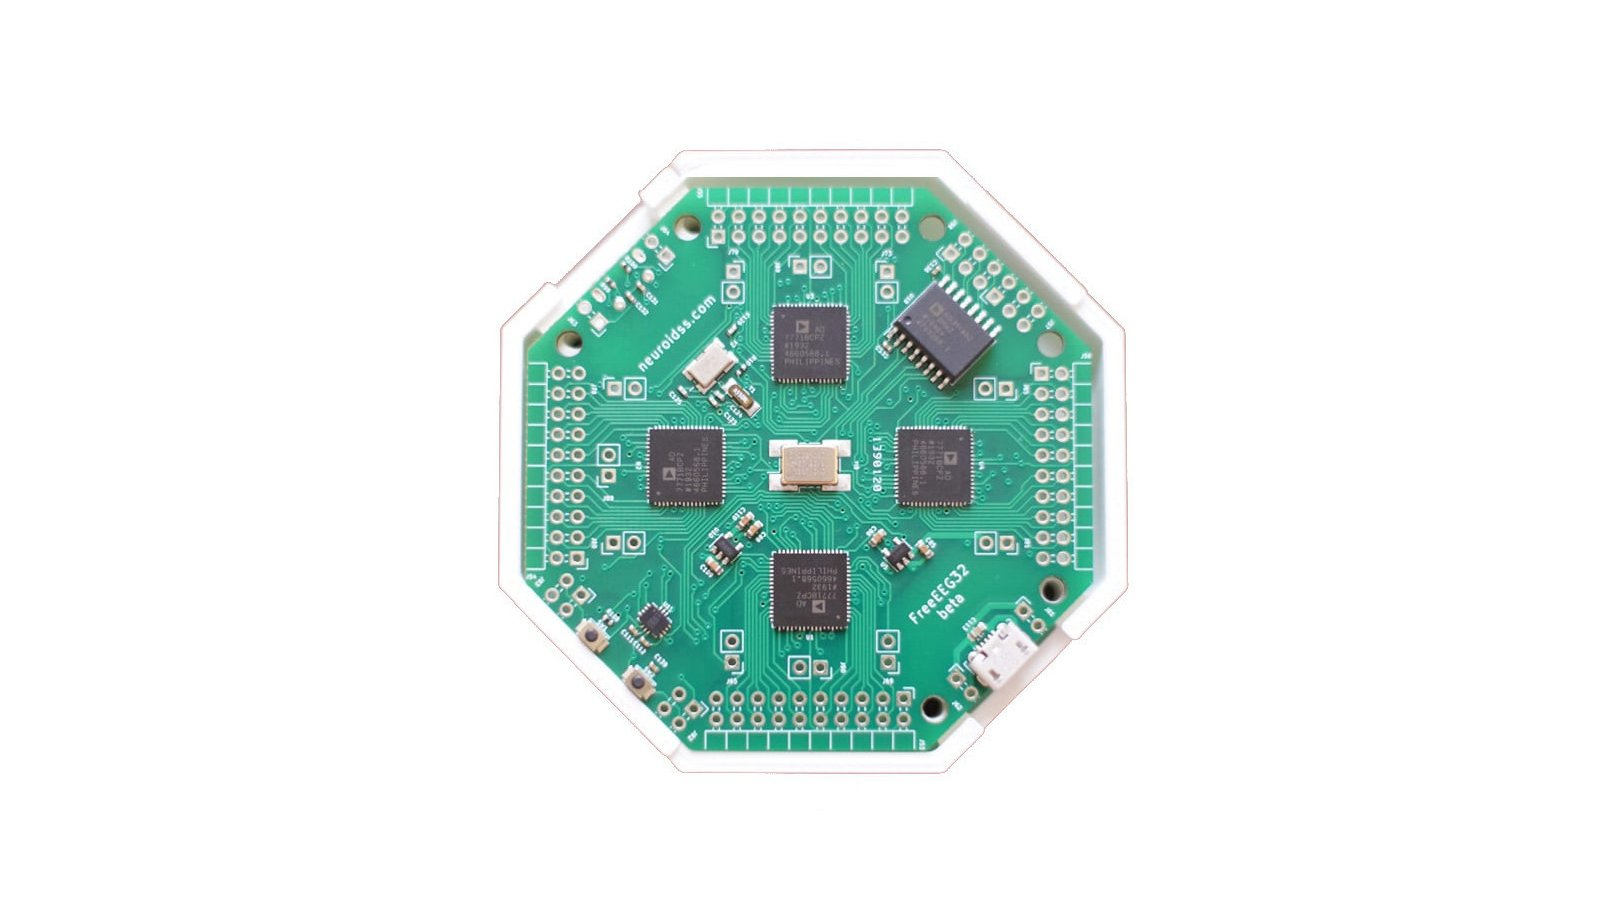
\includegraphics[width=\linewidth,height=21mm,keepaspectratio]{assets/history/freeeeg32-board.jpg}
      \par{\tiny FreeEEG32 acquisition board\par}\smallskip
      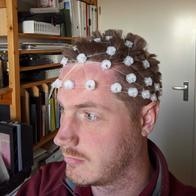
\includegraphics[height=25mm]{assets/people/bernard-markus-eeg-net.jpg}
      \par{\tiny Bernard Markus wearing his EEG net\par}
  \end{columns}
  {\tiny\color{NTXMuted}Sources: \href{https://icibici.github.io/site/}{icibici}; \href{https://www.crowdsupply.com/neuroidss/freeeeg32}{FreeEEG32}; \href{https://neurogate.io/}{Neurogate / OctaFlow}\par}
  \note{Photos: FreeEEG32 Crowd Supply campaign. Bernard Markus is identified in its team portrait, wearing his compatible net; no board connection is visible. Funded in 2021, the campaign now lists the board as discontinued. This is history, not a purchasing recommendation.}
  \note{[25:45--27:15] Morgan identifies these as community-supported projects. icibici credits NeuroTechX, Slack, and London Hackspace; Colin Rowat presented it at the 2023 hackathon. It is an engineering kit, not a consumer product, and warns against mains-connected use. Avoid historical price or cheapest claims. FreeEEG32 documents open-source 32-channel acquisition. Neurogate currently presents OctaFlow with EEG/EMG/ECG, LSL, and Timeflux; do not apply current specifications to all historical devices. These examples do not imply equivalent performance, licensing, clinical readiness, or safety for self-experimentation.}
\end{frame}

\begin{frame}{Open fNIRS: from accessible kits to research systems}
  \begin{columns}[c,onlytextwidth]
    \column{.56\textwidth}
      \small
  \NTXPoint{HEGduino --- Josh Brewster / Brains@Play}{Accessible optical sensing and biofeedback hardware.}
  \NTXPoint{OpenfNIRS}{Hardware, software, standards, and training; a directory including HEGduino and openNIRS.}
  \NTXPoint{ninjaNIRS --- Boston University}{Open, wearable, high-density fNIRS; system design and performance published in 2024.}
    \column{.40\textwidth}
      \centering
      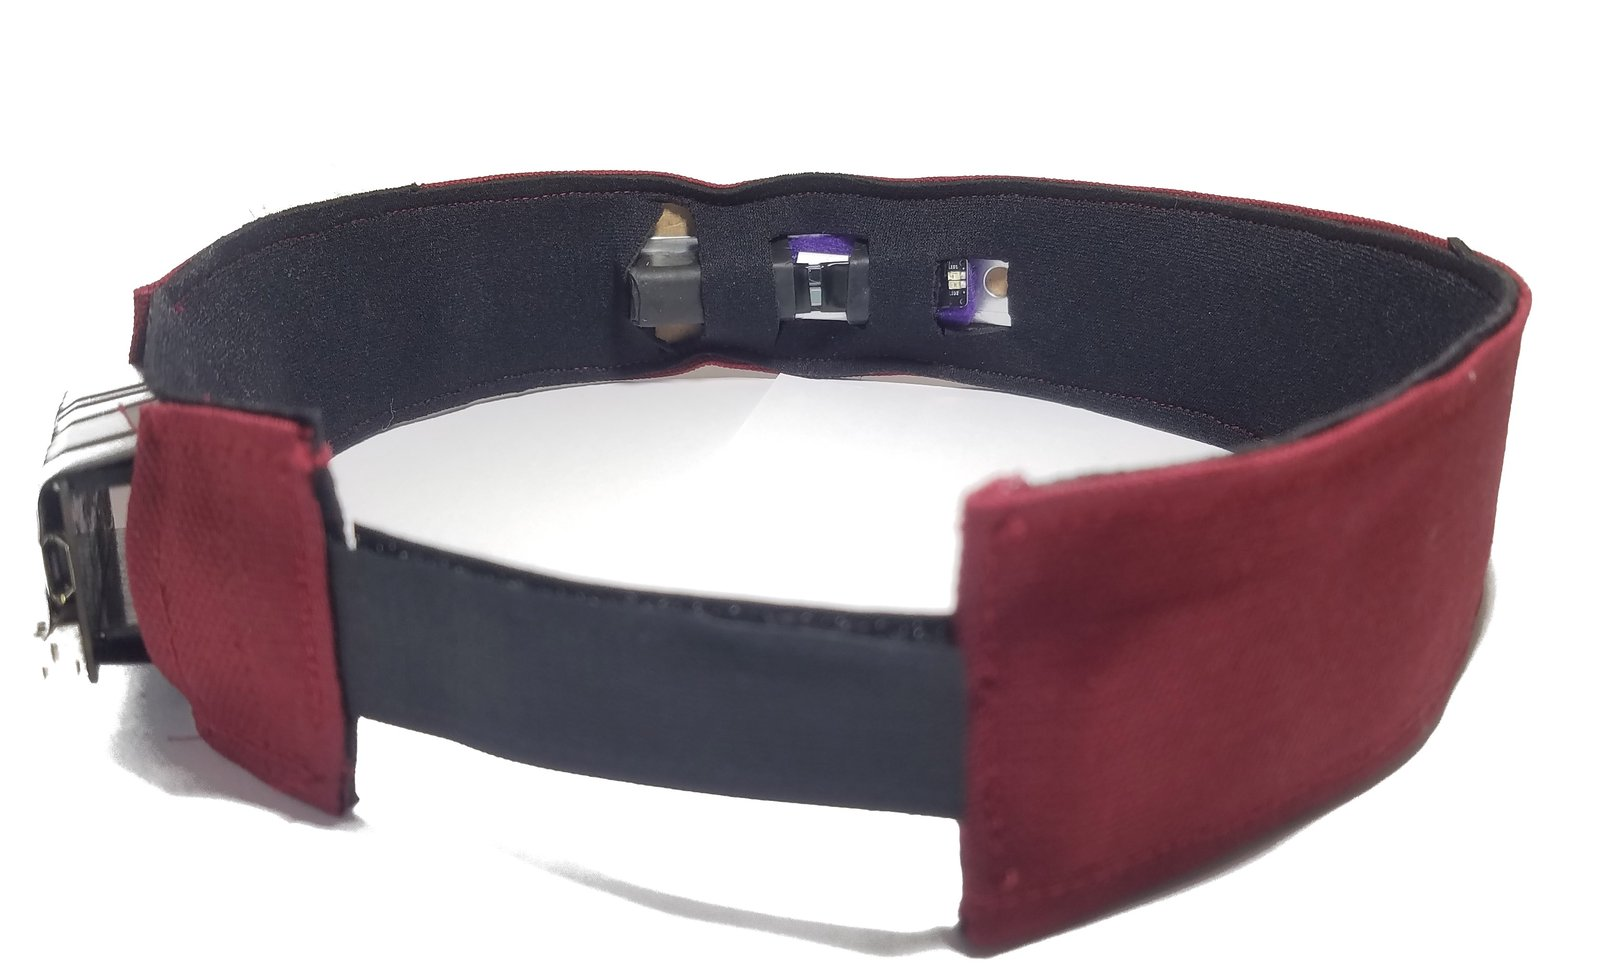
\includegraphics[width=\linewidth,height=22mm,keepaspectratio]{assets/history/hegduino-v2.jpg}\par
      {\tiny HEGduino V2 --- Alaskit / Crowd Supply\par}\smallskip
      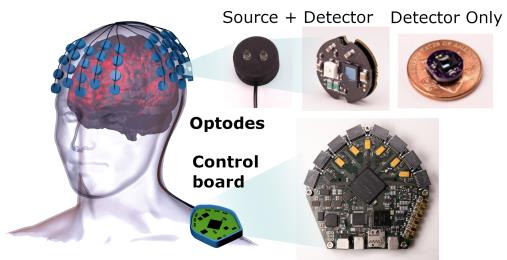
\includegraphics[width=\linewidth,height=23mm,keepaspectratio]{assets/history/ninjanirs-early-000.jpg}\par
      {\tiny Early ninjaNIRS --- \href{https://sites.bu.edu/nil/files/2020/04/AlexanderOSA.pdf}{von L\"uhmann et al., 2020}\par}
  \end{columns}
  {\scriptsize Community support connects entry-level learning with research tools.\par}
  {\tiny\color{NTXMuted}Sources: \href{https://www.crowdsupply.com/alaskit/hegduino-v2}{HEGduino V2}; \href{https://openfnirs.org/hardware/}{OpenfNIRS hardware}; \href{https://doi.org/10.1364/BOE.531501}{ninjaNIRS, Biomedical Optics Express, 2024}\par}
  \note{[27:15--28:45] Morgan supplies the account of NTX support for Josh Brewster's devices and interest in more research-oriented open fNIRS tools. The OpenfNIRS directory attributes HEGduino V2 to Joshua Brewster and Brains@Play. Distinguish the entry-level HEG/biofeedback kit from a high-density research fNIRS system; neither measures EEG. OpenfNIRS is the ecosystem, not one device; the directory separately lists Alexander von Luehmann's openNIRS 2015 hardware. ninjaNIRS is developed at Boston University's Neurophotonics Center, with its 2024 paper documenting wearable whole-head high-density hardware and performance characterization. Avoid equating affordability with equivalent sensitivity, channel coverage, or validation. No claim is made of NTX ownership, funding, or a formal partnership with Boston University or OpenfNIRS. Invite Morgan's firsthand examples of community support without inventing dates or outcomes.}
\end{frame}

\begin{frame}{Ultrasound hardware: another route into neurotech}
  \begin{columns}[c,onlytextwidth]
    \column{.55\textwidth}
      \small
      \NTXPoint{un0rick / pic0rick --- Luc Jonveaux}{Open pulse-echo hardware for learning, prototyping, and non-destructive testing.}
      \NTXPoint{Open-LIFU --- Openwater}{An open focused-ultrasound research platform: electronics, mechanical designs, firmware, planning, and simulation.}
      \NTXPoint{A place for community contributions}{Documentation, simulation, signal processing, and bench validation. Imaging and stimulation are different tasks.}
    \column{.41\textwidth}
      \centering
      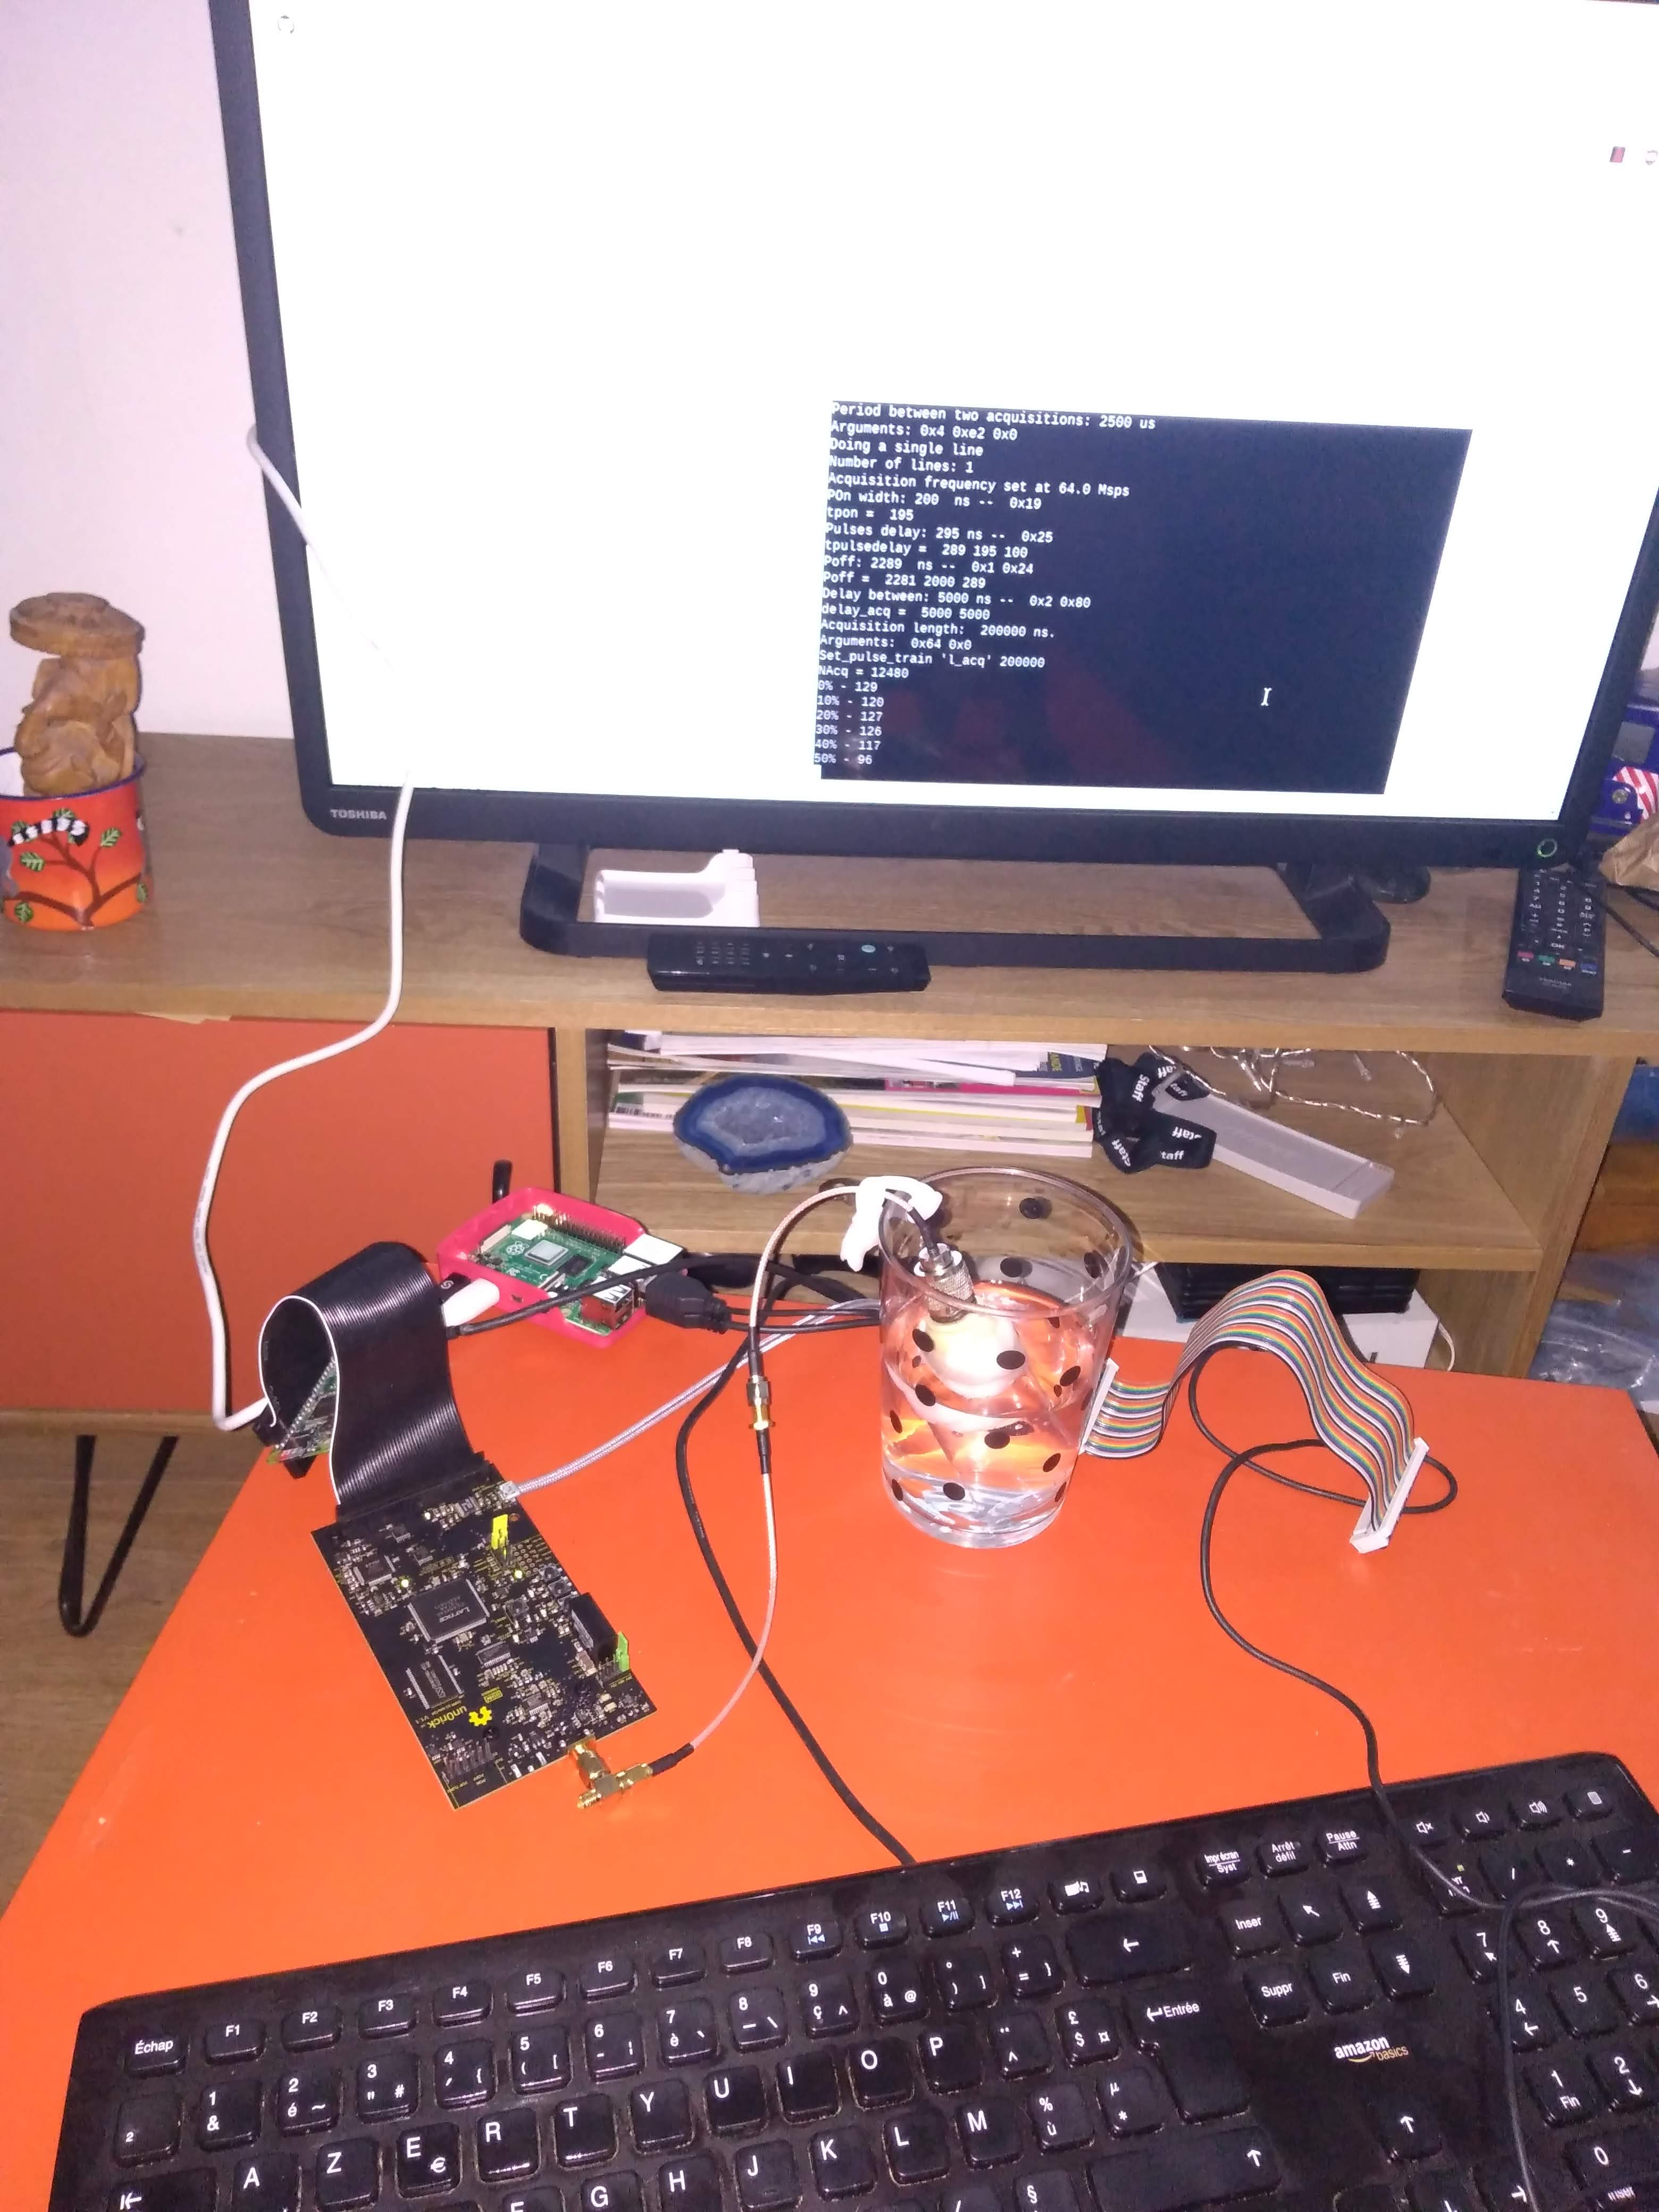
\includegraphics[width=\linewidth,height=43mm,keepaspectratio]{assets/history/un0rick-bench.jpg}\par\smallskip
      {\tiny Historical un0rick bench setup\newline Photo: Luc Jonveaux / kelu124, CC BY-SA 3.0\par}
  \end{columns}
  {\scriptsize Research hardware --- not a guide to self-administered brain stimulation.\par}
  {\tiny\color{NTXMuted}Sources: \href{https://un0rick.cc/}{un0rick open hardware}; \href{https://github.com/OpenwaterHealth}{Openwater platform repositories}\par}
  \note{[28:45--30:15] Expand the ultrasound example already introduced alongside OpenEIT. The un0rick lineage provides pulse-echo tools for learning and prototyping; the photograph shows a historical un0rick bench, not pic0rick or an Open-LIFU system. Openwater publishes separate focused-ultrasound research hardware and software repositories. Their inclusion illustrates available open research tools, not a claim that NTX owns, funds, or formally partners with either project. Do not imply that a pulse-echo board is interchangeable with a tFUS neuromodulation device or that low cost establishes diagnostic or clinical equivalence. Human stimulation requires appropriate research oversight, calibrated equipment, safety assessment, and qualified supervision. No operating parameters, human-use protocol, or claim of therapeutic efficacy is supplied. This leads into the local community that studies these methods together.}
\end{frame}

\begin{frame}{tFUS Society: a community around ultrasound}
  \begin{columns}[c,onlytextwidth]
    \column{.52\textwidth}
      \small
      \NTXPoint{Started with Leo Zaroff}{Bringing researchers, technical enthusiasts, and founders together around transcranial focused ultrasound.}
      \NTXPoint{Hosted by NeuroTechSF}{Meetings at Studio45/55 and Frontier Tower: talks, technical discussion, and shared projects.}
      \NTXPoint{From papers to shared work}{Project Sonus: ultrasound-imaging simulation and replication. Frontier Tower: a joint neuroimaging workshop with Lev Chizhov.}
    \column{.44\textwidth}
      \centering
      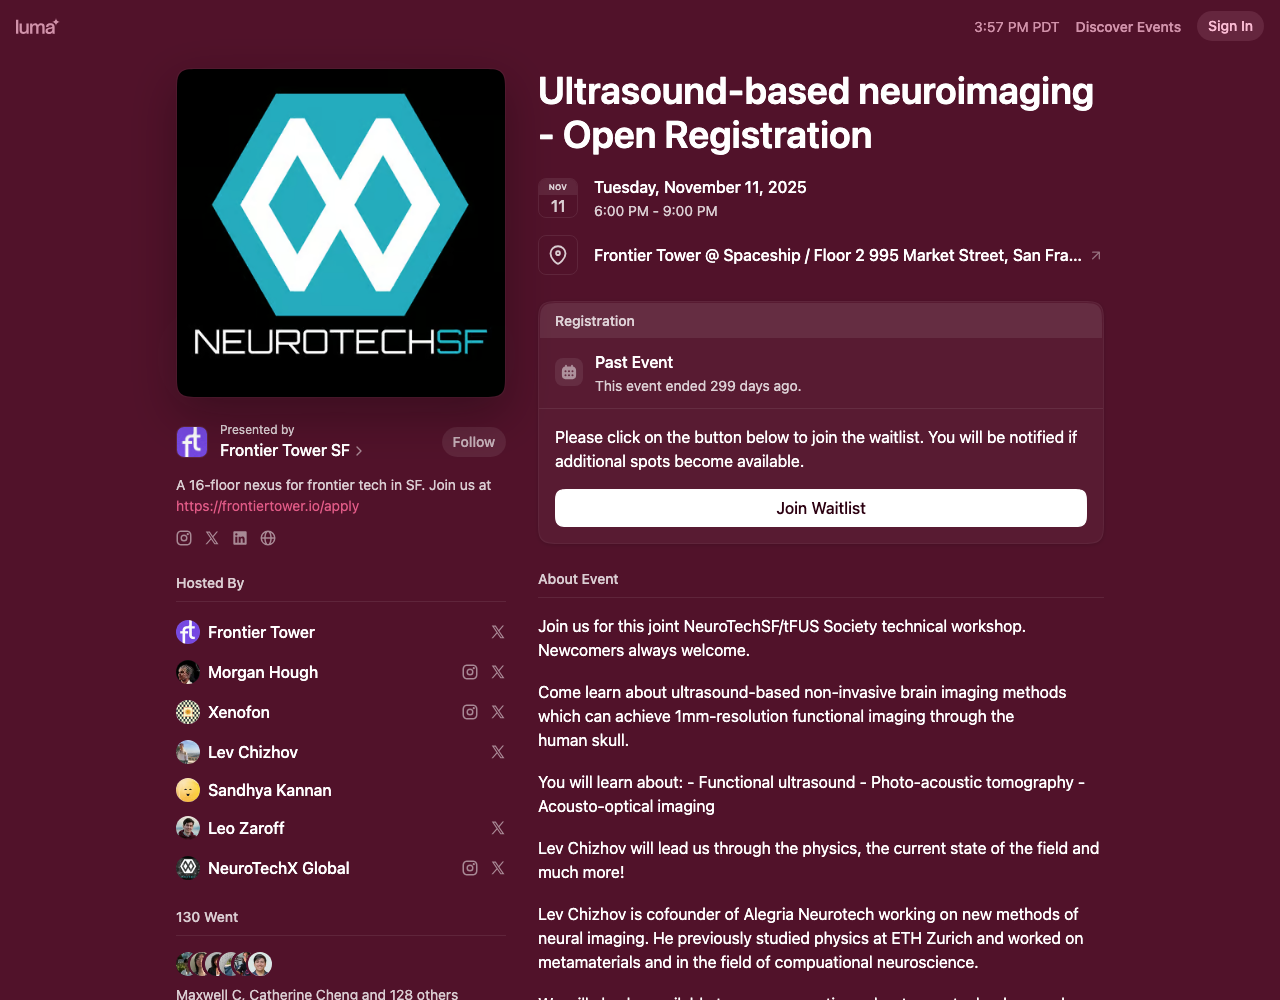
\includegraphics[width=\linewidth,height=46mm,keepaspectratio]{assets/history/tfus-frontier-event-page.png}\par\smallskip
      {\tiny Joint NeuroTechSF / tFUS Society workshop\newline Frontier Tower, November 11, 2025\newline Event-page screenshot --- not a meeting photograph\par}
  \end{columns}
  {\tiny\color{NTXMuted}Sources: \href{https://luma.com/e5kwzyvq}{Studio 55, November 6, 2024}; \href{https://luma.com/ultrasound-based-neuroimaging}{Frontier Tower workshop}; founding and Studio45 history: Morgan Hough\par}
  \note{[30:15--31:45] Morgan supplies the account that this was started with Leo and hosted by NeuroTechSF at Studio45/55 and Frontier Tower. Leo's public name is Leo Zaroff. His own April 2026 essay describes him as the founder of tFUS Society. Public Luma listings establish joint events and identify Morgan Hough, Leo Zaroff, and Nic Berry as hosts at the Studio 55 research-and-development meeting. Its local date is November 6, 2024 (UTC November 7). It describes Project Sonus as open-source simulation and replication of an academic full-waveform-inversion imaging paper; do not claim a completed working scanner or confuse imaging with stimulation. The November 11, 2025 Frontier Tower workshop lists Lev Chizhov and topics including functional ultrasound, photoacoustic tomography, and acousto-optical imaging. Its advertised resolution and safety claims are not independently adopted here. Studio 55 is verified in the public listing; Studio45 history is Morgan's supplied account, not an independently verified venue/date. RSVP labels are not audited attendance totals. No identifiable in-person meeting photo was located: the image is explicitly a screenshot of the actual event page. Replace it if Morgan supplies a verified event photograph.}
\end{frame}


\begin{frame}{Education: a way into the field}
  \begin{columns}[T,onlytextwidth]
    \column{.49\textwidth}
      \NTXPoint{The NeuroTech Primer}{An introduction to neurotechnology, including recording and stimulation.}
      \NTXPoint{Workshops and webinars}{Learn methods and hear from people working in the field.}
      \NTXPoint{Learning through contribution}{Developer meetings, open science, and shared projects.}
    \column{.46\textwidth}
      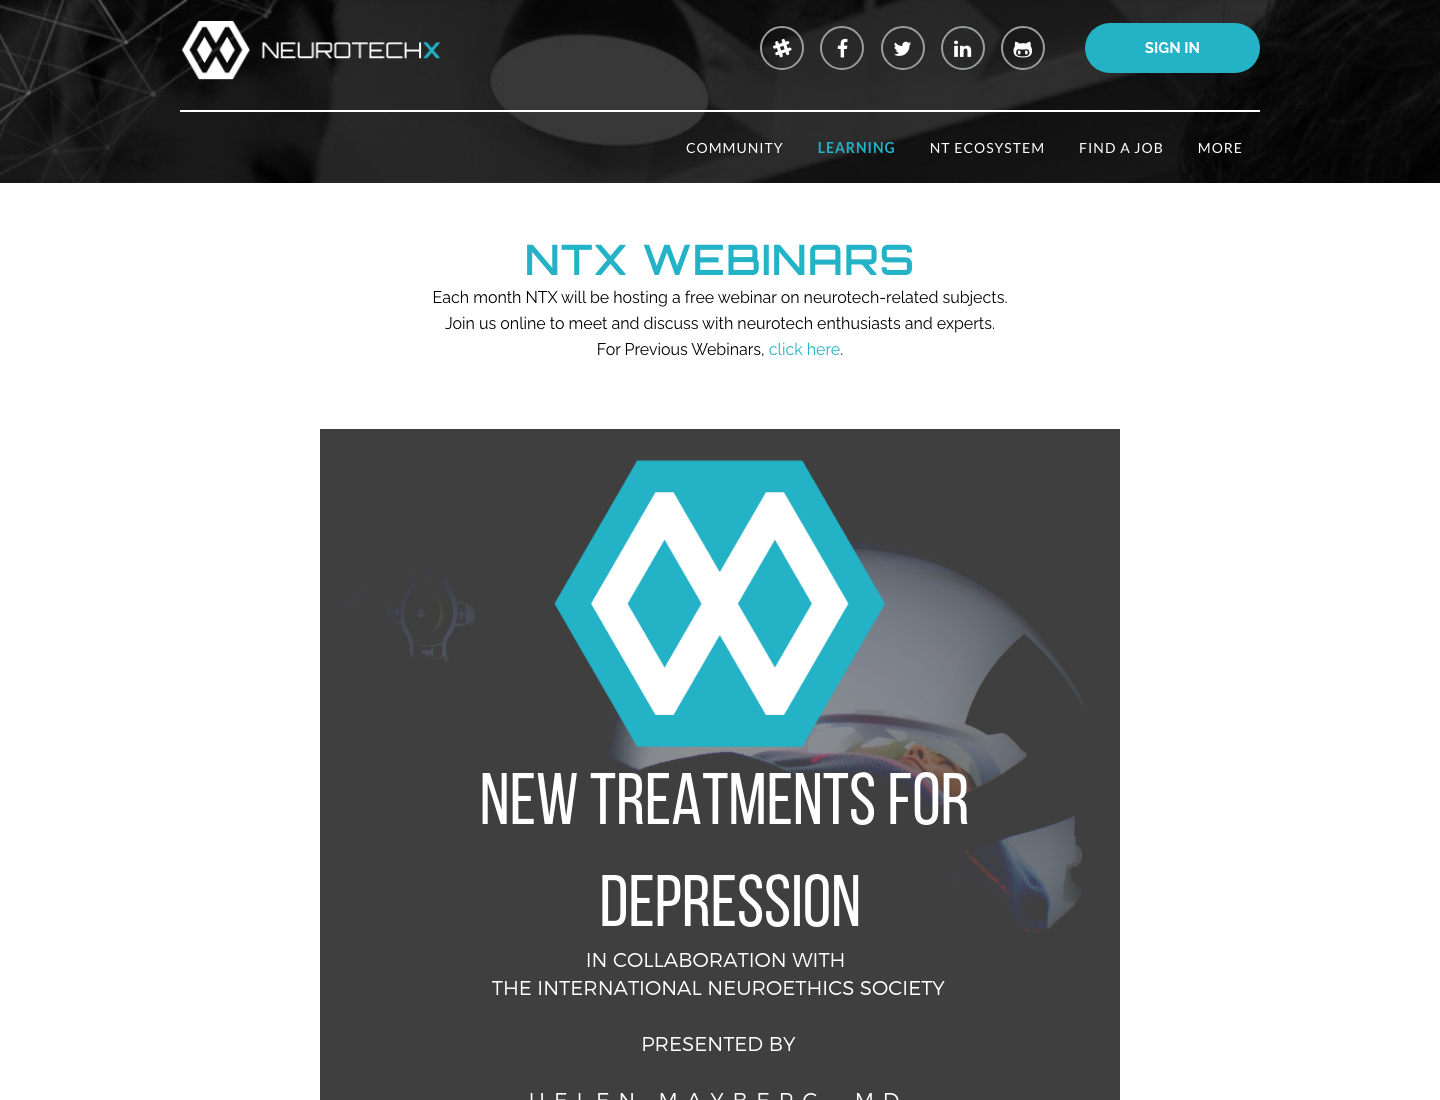
\includegraphics[width=\linewidth,height=46mm,keepaspectratio]{assets/history/neurotechx-webinar-page.png}
      \par\smallskip{\scriptsize \href{https://neurotechx.com/webinar/}{neurotechx.com/webinar}\par}
  \end{columns}
  \NTXSource{https://www.neurotechx.org/education}{NeuroTechX: The NeuroTech Primer, learning resources, and developer meetings}
  \note{[31:45--32:25] Connect this to the book and education slides in your original deck. These are several routes into participation, without claiming that every learner follows the same path. Not every resource linked on the education page was created by NeuroTechX. The right-hand visual is an authentic screenshot of neurotechx.com/webinar captured September 6, 2026. It illustrates the webinar resource, not a current event announcement. The page describes monthly webinars; distinguish this series from the weekly online pandemic Hacknights described by Morgan. The Primer cover asset remains in the repository.}
\end{frame}

\section{How do we add to the community?}
\NTXDivider{Students Are the Future}
\begin{frame}{A competition that helped organize student clubs}
  \begin{columns}[T,onlytextwidth]
    \column{.49\textwidth}
      \NTXPoint{2016: a five-club pilot}{Montr\'eal and Toronto; a November Demo Day in Montr\'eal.}
      \NTXPoint{A reason to organize}{The annual competition helped students establish university clubs.}
      \NTXPoint{A shared goal}{Build a project and show the work.}
    \column{.46\textwidth}
      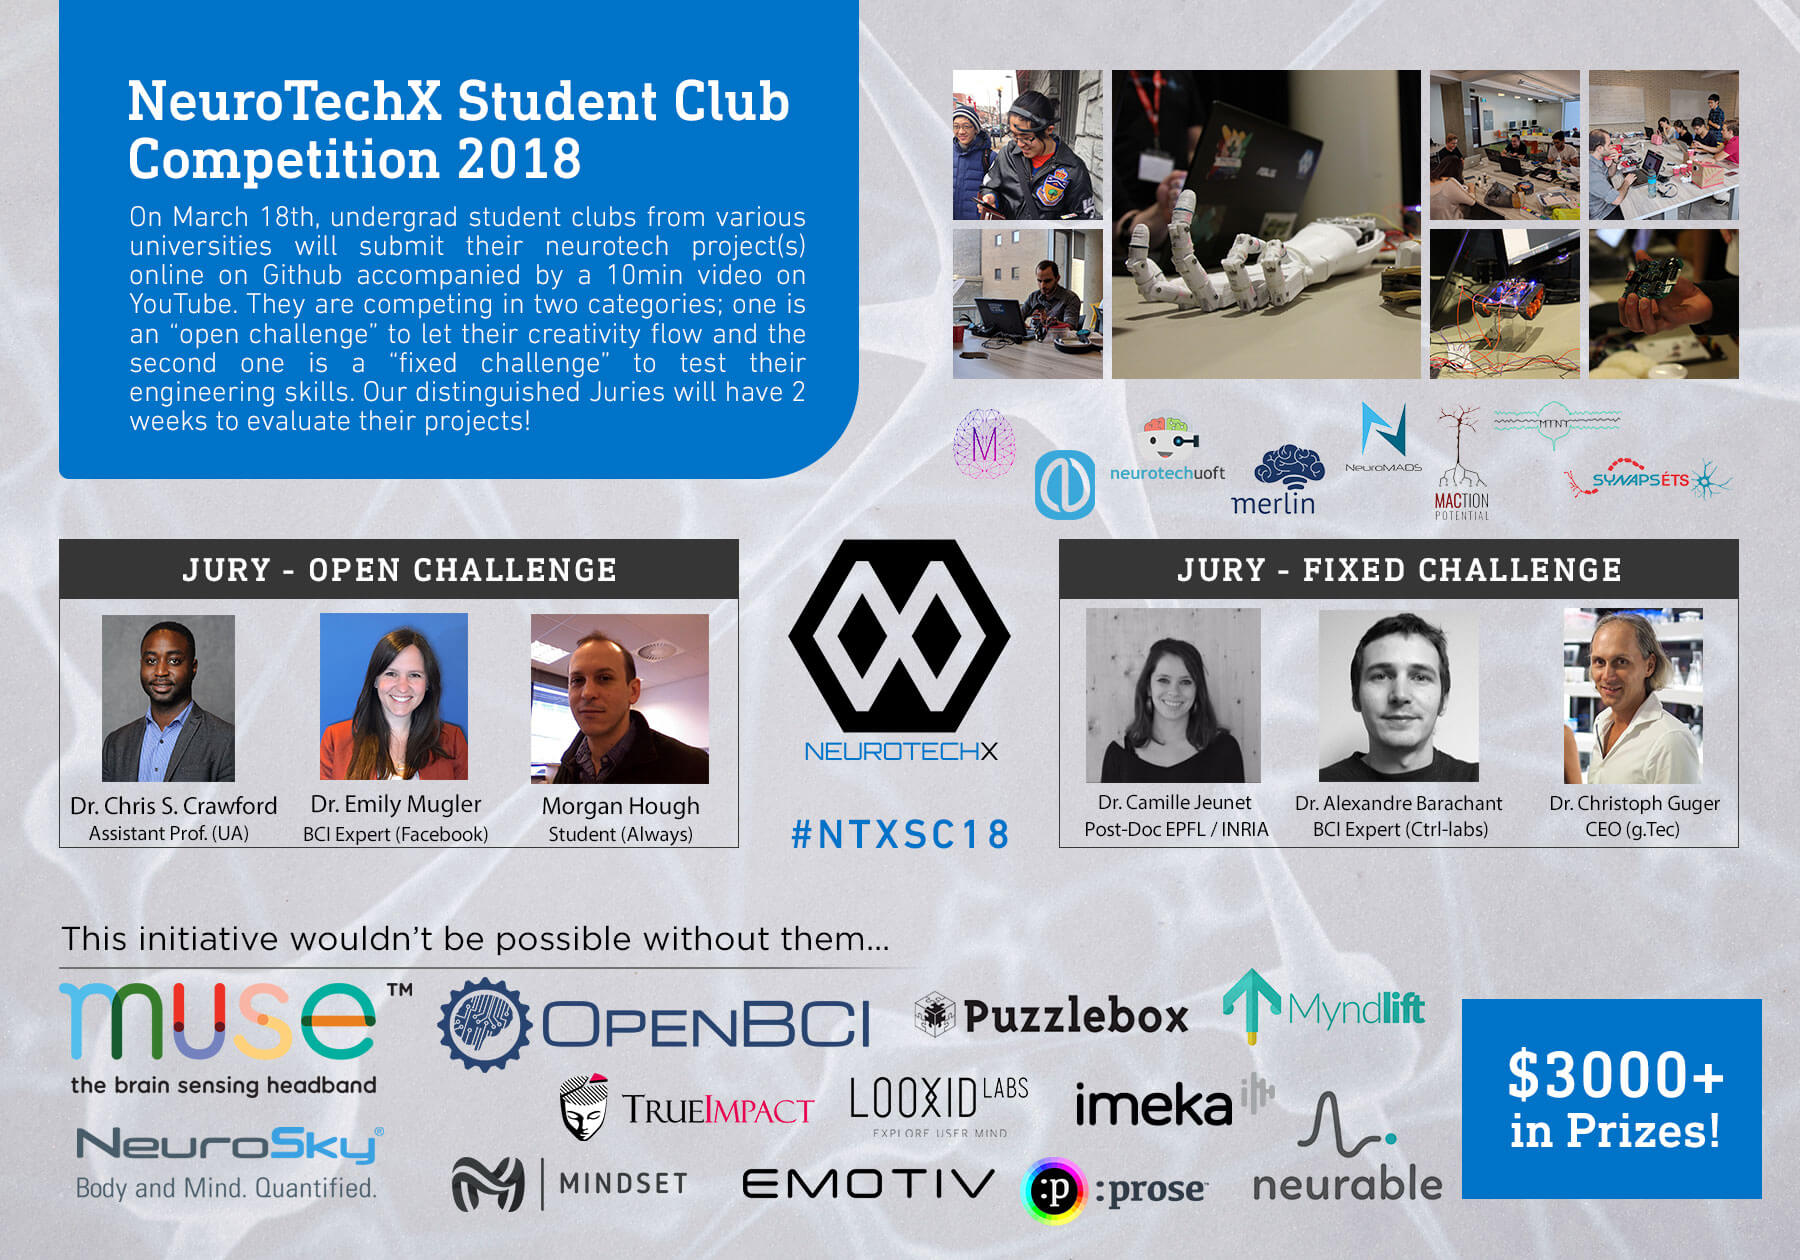
\includegraphics[width=\linewidth,height=44mm,keepaspectratio]{assets/history/student-competition-2018-flyer.jpg}
      \par\smallskip{\scriptsize Original 2018 competition announcement\par}
  \end{columns}
  {\tiny\color{NTXMuted}Sources: \href{https://medium.com/neurotechx/ntx-student-clubs-initiative-2fba98b0d082}{NeuroTechX's 2017 retrospective}; \href{https://neurotechx.com/ntx-student-clubs-competition/}{2018 announcement}\par}
  \note{[32:25--33:05] The retrospective explicitly connects the competition to helping students organize university clubs. Its 2016 pilot included SynapsETS, MENTAL, BSYS, PolyCortex, and NeuroTechUofT. The visual is the later 2018 flyer, not a 2016 Demo Day photograph. Morgan's lesson: the annual competition became an organizing function for student chapters. Keep this distinct from global hackathons and regional conferences.}
\end{frame}

\begin{frame}{Student participation: people and projects}
  \begin{columns}[c,onlytextwidth]
    \column{.58\textwidth}
      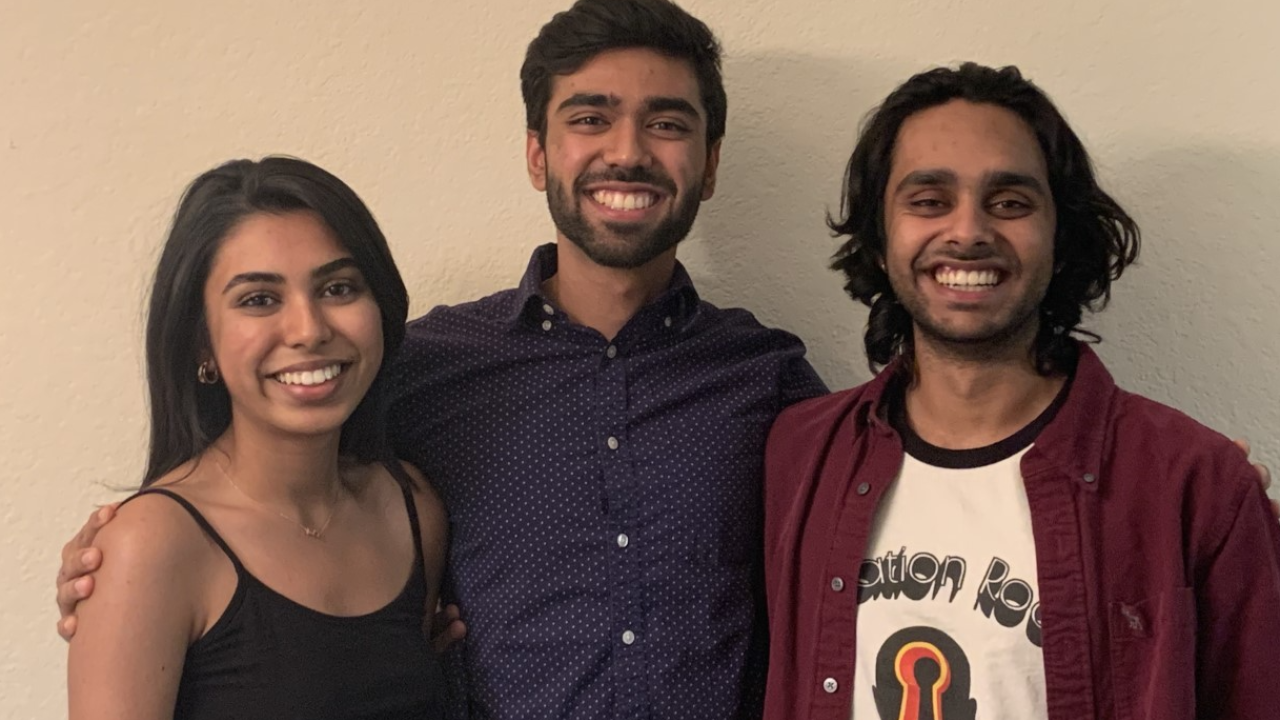
\includegraphics[width=\linewidth,height=37mm,keepaspectratio]{assets/chapters/uc-davis-neuroassist-team-2020.png}
      \par\smallskip{\small Neurotech@Davis: the NeuroAssist team\par}
    \column{.36\textwidth}
      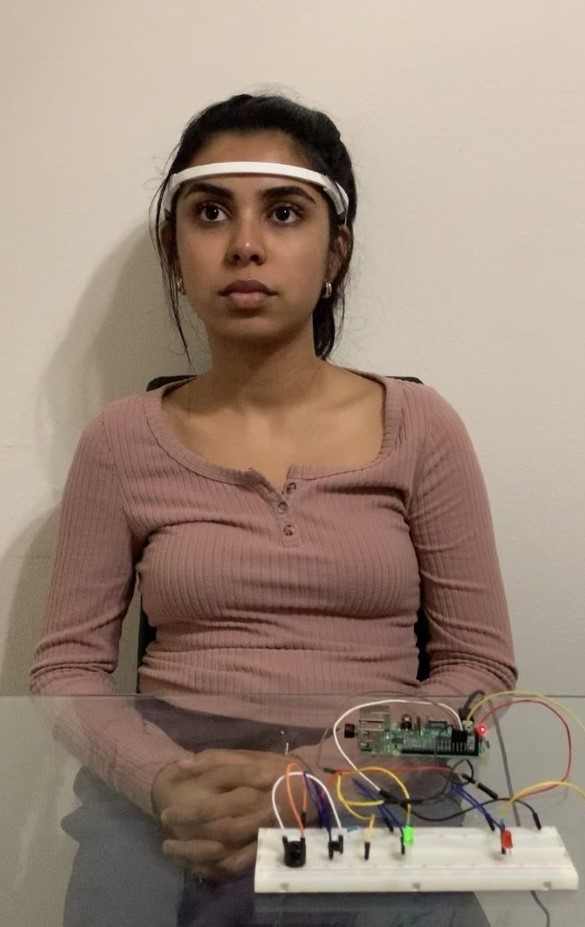
\includegraphics[width=\linewidth,height=37mm,keepaspectratio]{assets/chapters/uc-davis-neuroassist-headset-2020.jpg}
      \par\smallskip{\small Priyanshi wearing NeuroAssist\par}
  \end{columns}
  \medskip
  {\small Built for the 2020 NeuroTechX Student Competition.\par}
  \NTXSource{https://neuroengineering.ucdavis.edu/news/neurotechdavis-student-club-undergraduate-students-learn-about-neurotechnology}{Photos and identification: Neuroengineering at UC Davis, April 2022}
  \note{[33:05--33:45] UC Davis identifies the team as Priyanshi, Kushaal, and Ayush and both photographs with the 2020 NeuroAssist competition project. The article was published in 2022; do not label these as photographs taken at a 2022 competition. Use this as a concrete example of student participation, not a clinical efficacy claim or proof of every club's experience.}
\end{frame}

% Historical events are part of the main presentation, not an addendum.
% Allow approximately one minute each: 13:00--16:00.
\begin{frame}{The global hackathon: 2022}
  \begin{columns}[c,onlytextwidth]
    \column{.44\textwidth}
      \small
      \NTXPoint{October 29--30, 2022}{Free, global online participation with local chapter hosting.}
      \NTXPoint{Brain-age prediction from EEG}{Child Mind Institute's Healthy Brain Network (HBN) dataset.}
      \NTXPoint{A shared challenge platform}{Paris-Saclay's CodaLab; Sylvain Chevallier's MNE / scikit-learn starting kit.}
    \column{.52\textwidth}
      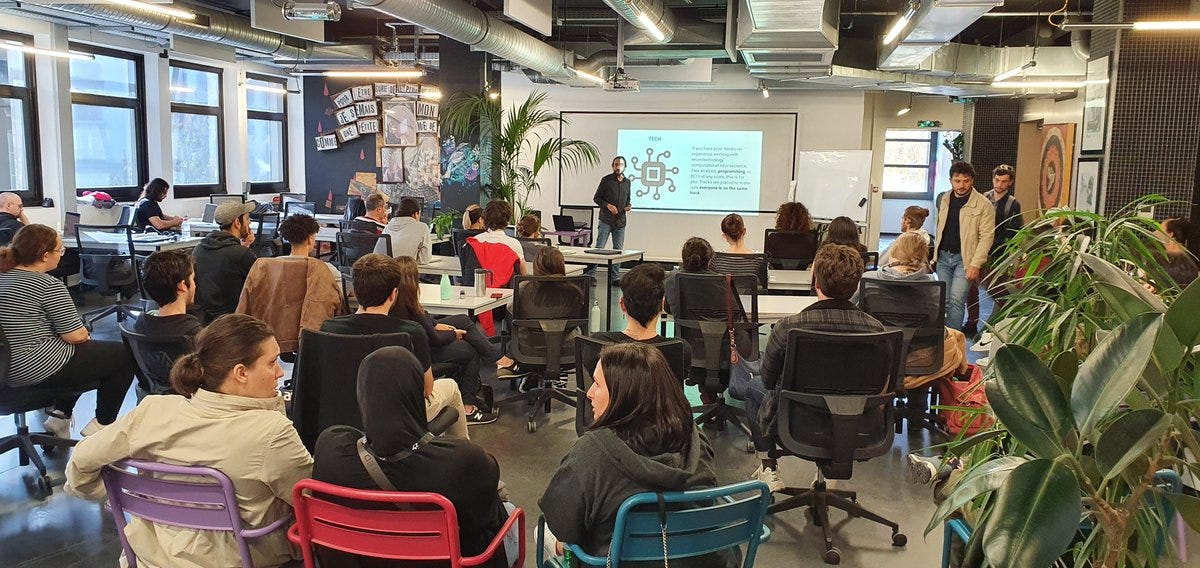
\includegraphics[width=\linewidth,height=44mm,keepaspectratio]{assets/chapters/paris-global-hackathon-2022.jpg}
      \par\smallskip{\scriptsize Briefing session in Paris\par}
  \end{columns}
  {\tiny\color{NTXMuted}Sources: \href{https://tailor-network.eu/brain-age-prediction-challenge/}{TAILOR}; \href{https://codalab.lisn.upsaclay.fr/competitions/8336}{CodaLab}; \href{https://gist.github.com/sylvchev/206f93acd7393ab3b955602eba42d427}{starting kit}; HBN: Morgan Hough; photo: NTX Content Lab / Firas Safieddine\par}
  \note{The photo is captioned Briefing session in Paris in the official Content Lab retrospective, published December 3, 2022. The program advertised five locations; the later retrospective reports six including New York. Do not confuse the advertised list with a final attendance audit.}
  \note{[33:45--34:45] Historical context, approximately one minute. Morgan identifies the data task as brain-age prediction using Child Mind Institute Healthy Brain Network EEG and confirms CodaLab as the platform. TAILOR's November 16, 2022 announcement verifies the brain-age task and Paris-Saclay CodaLab competition 8336; it gives November 4--22 as the challenge window, distinct from the October 29--30 hackathon. Sylvain's October 30 starting kit uses MNE, scikit-learn pipelines, PCA, and ridge regression. This was an EEG machine-learning challenge, not a deep-learning-only contest or a clinically validated brain-age diagnostic. The Content Lab retrospective credits Inria, TAILOR, Universite Paris-Saclay, and LISN. Do not confuse this with the separate RAMP/OpenBHB MRI brain-age challenge. Earlier hosting details remain in the source archive.}
\end{frame}

\begin{frame}{The global hackathon: 2023}
  \begin{columns}[c,onlytextwidth]
    \column{.44\textwidth}
      \small
      \NTXPoint{December 2--3, 2023}{Second annual global event: free and hybrid.}
      \NTXPoint{Eight advertised locations}{Paris, Vienna, Zurich, Delhi, Kharagpur, Bras\'{i}lia, Buenos Aires, London.}
      \NTXPoint{Four tracks}{Hardware; data; design and strategy; new ethics track.}
    \column{.52\textwidth}
      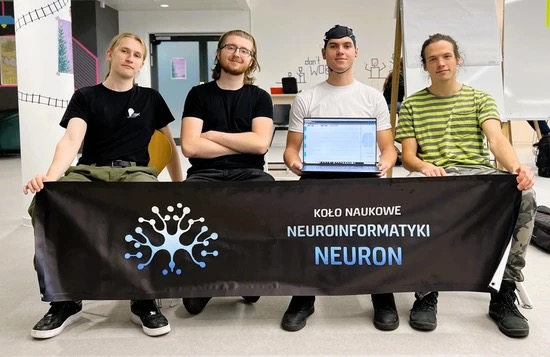
\includegraphics[width=\linewidth,height=42mm,keepaspectratio]{assets/chapters/vienna-global-hackathon-2023.jpg}
      \par\smallskip{\scriptsize Neuron club team, Vienna\newline ``Bore No More'' --- second in software\par}
  \end{columns}
  \smallskip{\scriptsize Historically coordinated with \'Ecole 42 across multiple cities.\par}
  {\tiny\color{NTXMuted}Sources: \href{https://neurotechx.com/hackathon2023/}{2023 program}; photo: \href{https://wit.pwr.edu.pl/en/news/students-from-the-neuron-club-successful-in-ntx-hackathon-163.html}{Wroc\l{}aw University of Science and Technology}; coordination: Morgan Hough\par}
  \note{[34:45--35:45] Historical context, approximately one minute. The 2023 program lists eight host cities and adds ethics as a fourth track; advertised locations do not establish attendance or growth. Morgan confirms historical multi-city coordination with Ecole 42; both official event pages display its sponsor logo, but no specific campus list or exclusive organizing role is inferred. The university recap identifies Neuron students Pawel Dzikiewicz, Tomasz Koralewski, Jakub Ner, and Adam Pawlowski presenting Bore No More in Vienna and placing second in software. This is the global hackathon, not the separate student club competition. No generalizable classifier-performance or clinical claim is made. Photo provenance is recorded in assets/chapters/event-photo-sources.md.}
\end{frame}

% Historical addition to Morgan's Google Slides deck.
% Suggested placement: after "Global NeuroTechX Community".
\begin{frame}{Global NeuroHack 2026}
  \textbf{April 10--12, 2026}\par
  Frontier Tower, San Francisco\par\bigskip

  A recent event we hosted, with NeuroTechX helping organize\newline
  and support the hackathon.\par\bigskip

  Three tracks:
  \begin{itemize}
    \item Blue-Sky Prototyping
    \item Non-Implantable Speech Decoding
    \item Maximizing Bit Rate
  \end{itemize}
  \medskip
  The program included workshops, mentor check-ins,\newline
  and project presentations.\par\medskip
  {\scriptsize\href{https://global-neurohack.github.io/}{global-neurohack.github.io}\par}
  \note{Historical context, approximately one minute. Morgan identified this as a recent event NeuroTechX hosted. The event website supplies the date, venue, tracks, and program, and credits NeuroTechX with organizing support. Its copy remains prospective: do not present advertised attendance, country counts, mentor counts, or scheduled activities as independently verified outcomes. Morgan's firsthand account should supply actual turnout, memorable projects, what worked, what did not, and any subsequent collaborations. No lesson or outcome has been invented here.}
\end{frame}


\section{NeuroTechX loves DLEEG}
\NTXDivider{NeuroTechX\,$\heartsuit$\,DLEEG}

\begin{frame}{MOABB: making BCI comparisons reproducible}
  \begin{columns}[c,onlytextwidth]
    \column{.43\textwidth}
      \small
      \NTXPoint{Mother of All BCI Benchmarks}{Open comparisons on public EEG datasets.}
      \NTXPoint{The 2024 benchmark study}{30 pipelines, 36 datasets:\newline motor imagery, P300, and SSVEP.}
      \NTXPoint{A shared research foundation}{Implementations and evaluations others can inspect and reproduce.}
    \column{.53\textwidth}
      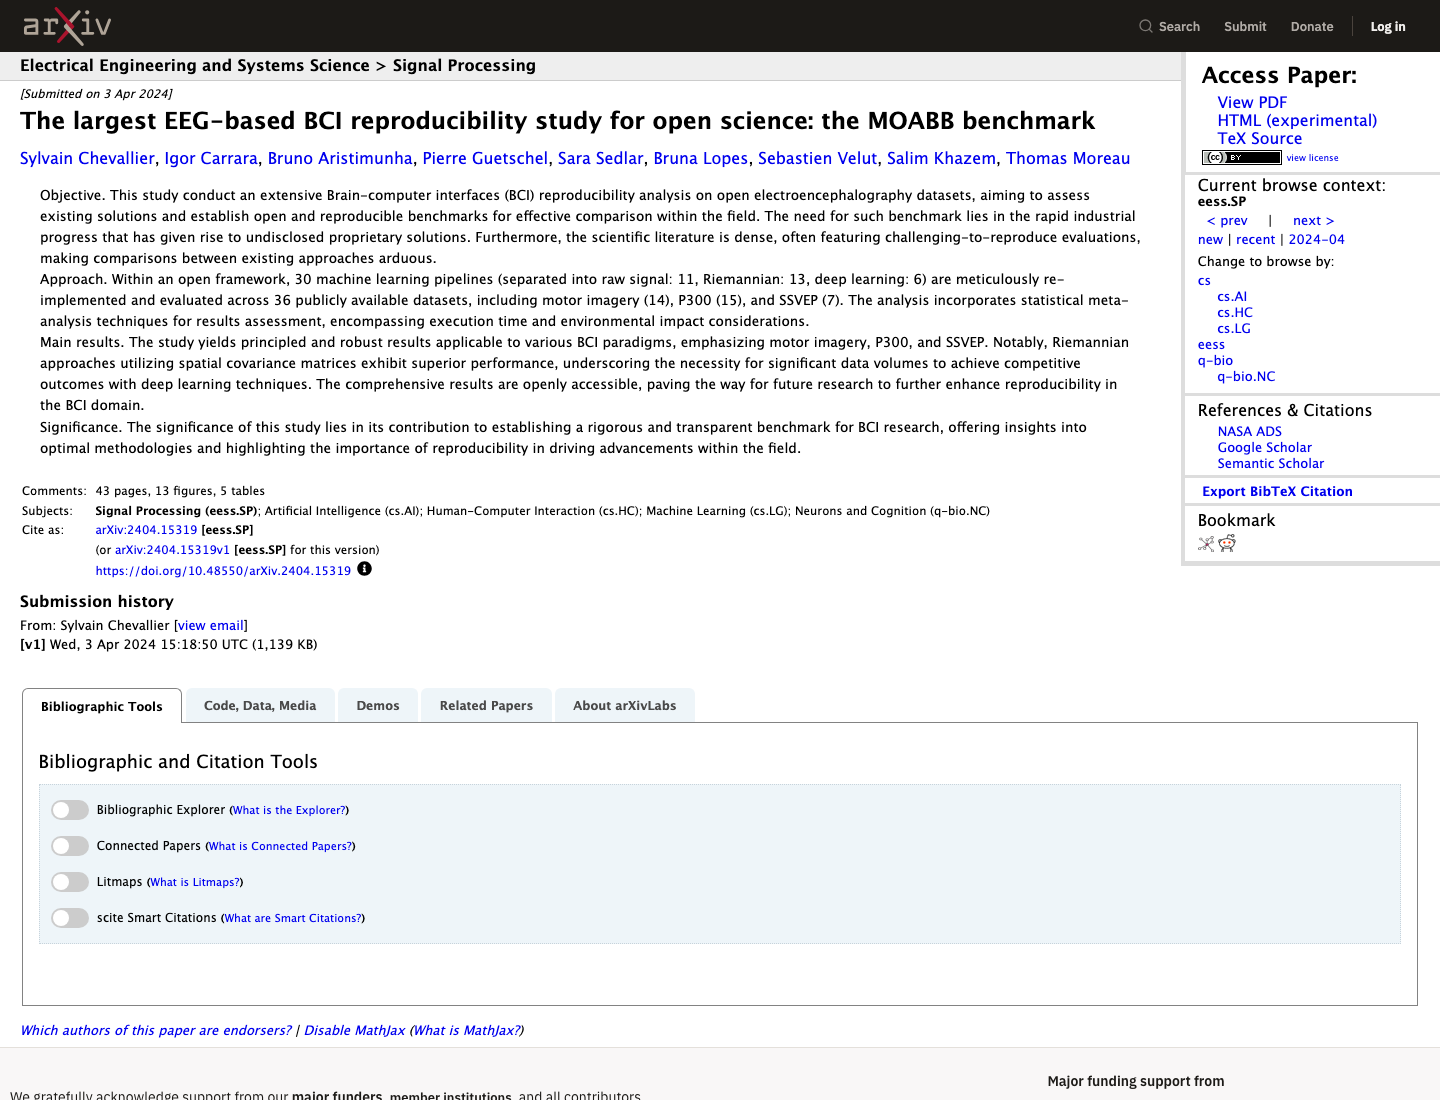
\includegraphics[width=\linewidth,height=45mm,keepaspectratio]{assets/history/moabb-arxiv-abstract.png}
      \par\smallskip{\scriptsize The MOABB benchmark --- arXiv abstract page\par}
  \end{columns}
  \NTXSource{https://arxiv.org/abs/2404.15319}{Chevallier et al., 2024, arXiv:2404.15319}
  \note{[36:45--38:15] MOABB is an example of community work producing a research artifact beyond a single event. The numerical scope is specific to the cited 2024 study, not today's dataset total. Credit the contributors. Do not generalize the study into a claim that a particular algorithm always wins or that benchmark performance establishes clinical utility.}
\end{frame}

\begin{frame}{Shared tools, shared teaching: a path into DLEEG}
  \begin{columns}[c,onlytextwidth]
    \column{.58\textwidth}
      \small
      \NTXPoint{An interoperable Python ecosystem}{MNE: EEG processing. scikit-learn: pipelines and evaluation. pyRiemann: covariance-based learning.}
      \NTXPoint{Pedro Rodrigues and Sylvain Chevallier}{Hands-on teaching with reusable notebooks: \href{https://github.com/plcrodrigues/Workshop-MOABB-BCI-Graz-2019}{Graz 2019} and the \href{https://github.com/mccorsi/BCI-2023-Open-Source-Tool-workshop}{2023 open-source BCI workshop}.}
      \NTXPoint{The next generation carries it forward}{Istanbul, MLSP 2025: Bruno Aristimunha co-organized with Sylvain, Florian Yger, and Marie-Constance Corsi.}
    \column{.38\textwidth}
      \centering
      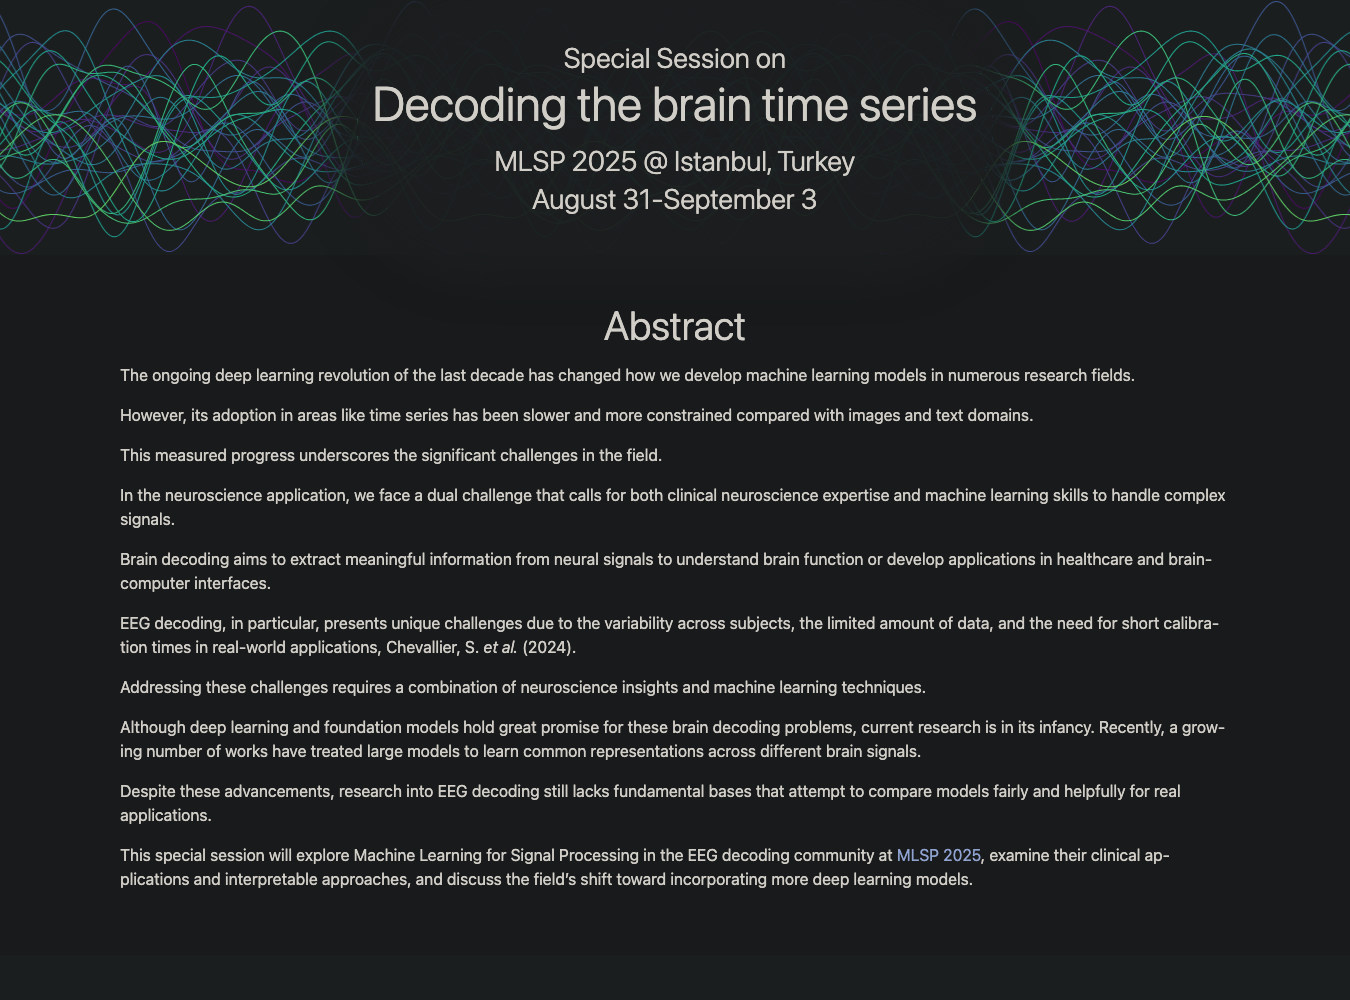
\includegraphics[width=\linewidth,height=42mm,keepaspectratio]{assets/history/dleeg-istanbul-workshop.png}\par\smallskip
      {\tiny Decoding the brain time series\newline Istanbul, August 31--September 3, 2025\newline Official special-session page\par}
  \end{columns}
  {\tiny\color{NTXMuted}Sources: linked workshop repositories; \href{https://mlsp2025-decoding-brain.github.io/}{MLSP 2025}; \href{https://bruaristimunha.github.io/}{Bruno Aristimunha}. DLEEG = deep learning for EEG.\par}
  \note{[38:15--39:45] Start with the ecosystem that makes rigorous EEG machine learning teachable. MNE handles EEG data and preprocessing; scikit-learn supplies reusable estimators, pipelines, and evaluation; pyRiemann brings covariance geometry into this ecosystem. These are broader than deep learning and provide useful baselines. Pedro is Pedro L. C. Rodrigues. His Graz 2019 repo explicitly teaches these tools with MOABB. The 2023 workshop lists Sylvain on MOABB and Pedro on pyRiemann; do not attribute every workshop exclusively to them. Also see the lkorczowski/BCI-2021-Riemannian-Geometry-workshop repository. Istanbul was a special session within IEEE MLSP 2025, not a standalone NTX training workshop. Its organizers include Bruno, Florian, Marie-Constance, and Sylvain; Hubert Banville was the announced keynote speaker. Bruno's own biography identifies Sylvain, Marie-Constance, and Raphael de Camargo as his PhD advisors. He illustrates the next generation; do not label all co-organizers as Sylvain's students or assert that NTX owns these libraries.}
\end{frame}

\begin{frame}{Yannick Roy and colleagues: mapping deep learning for EEG}
  \begin{columns}[c,onlytextwidth]
    \column{.47\textwidth}
      \small
      \NTXPoint{A systematic review, 2019}{\emph{Deep learning-based electroencephalography analysis: a systematic review.}}
      \NTXPoint{Across application areas}{Epilepsy, sleep, BCI, and cognitive and affective monitoring.}
      \NTXPoint{A community research agenda}{Share data and code; strengthen reproducibility and comparisons between methods.}
    \column{.49\textwidth}
      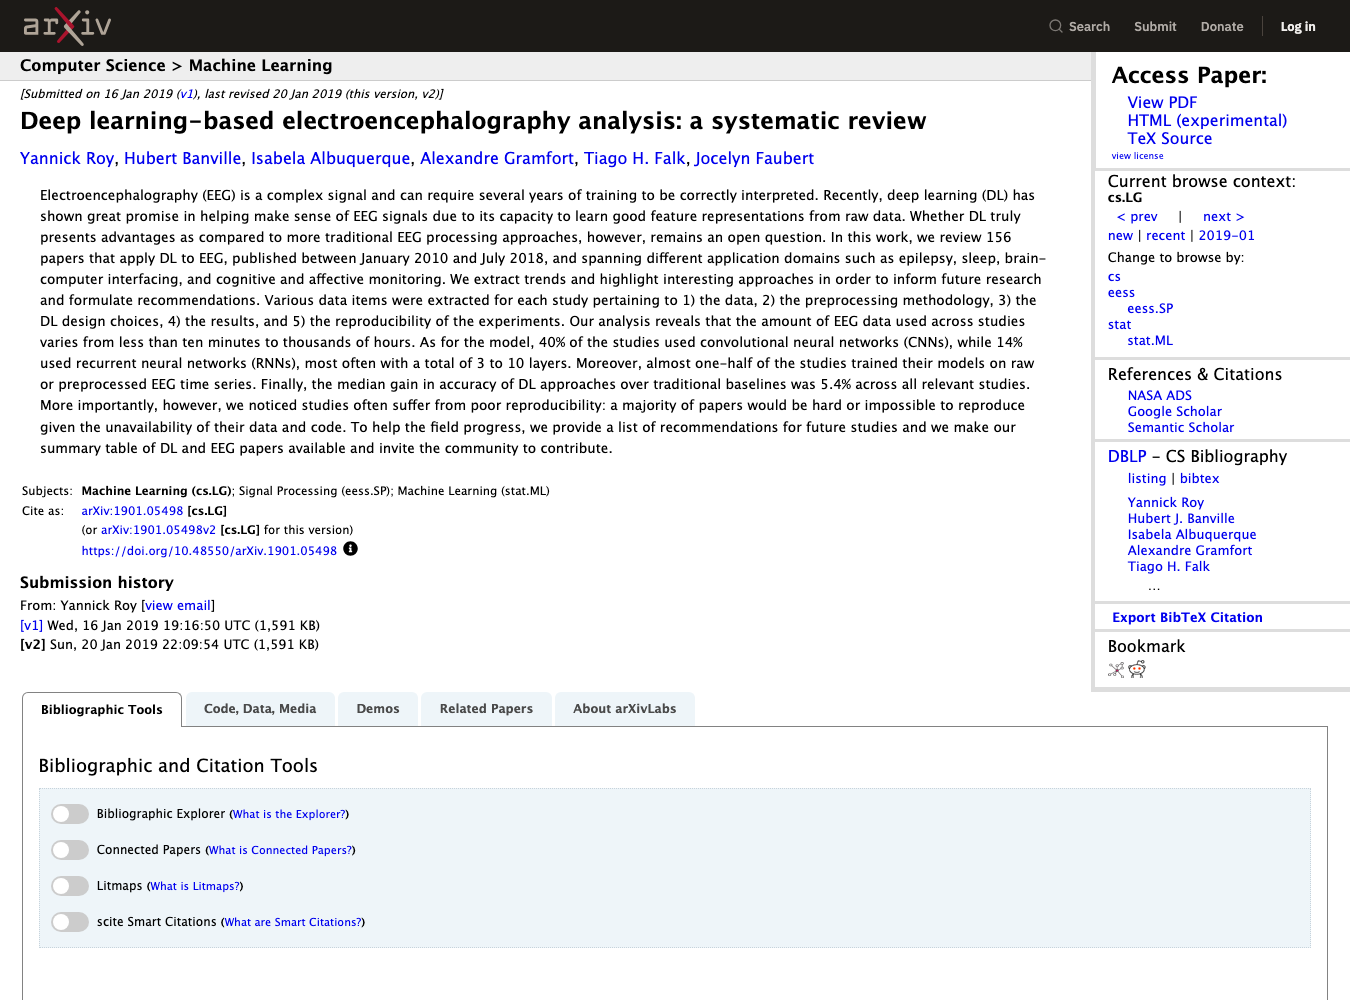
\includegraphics[width=\linewidth,height=45mm,keepaspectratio]{assets/history/dleeg-roy-article-page.png}\par\smallskip
      {\tiny Article's arXiv abstract page\newline Roy, Banville, Albuquerque, Gramfort, Falk, Faubert\par}
  \end{columns}
  {\tiny\color{NTXMuted}Sources: \href{https://arxiv.org/abs/1901.05498}{arXiv:1901.05498}; \href{https://doi.org/10.1088/1741-2552/ab260c}{Journal of Neural Engineering 16, 051001 (2019)}\par}
  \note{[39:45--41:15] Credit all authors: Yannick Roy, Hubert Banville, Isabela Albuquerque, Alexandre Gramfort, Tiago H. Falk, and Jocelyn Faubert. The review covers work published from January 2010 to July 2018 and emphasizes reproducibility and data/code availability. The displayed image is a genuine arXiv article-page screenshot, not the journal publisher's page. Its preprint abstract reports 156 papers; the published abstract indexed in PubMed reports 154, so the slide deliberately does not mix counts across versions. This is a review and research agenda, not a new model or evidence that deep learning always beats classical pipelines. Connect Yannick's work with the workshops and open tools without inventing a formal causal relationship between the review and later challenges.}
\end{frame}

\begin{frame}{Neureka 2020: community, clinical EEG, shared evaluation}
  \begin{columns}[c,onlytextwidth]
    \column{.58\textwidth}
      \small
      \NTXPoint{NeuroTechX + Novela Neurotech}{A global epilepsy challenge built around automatic seizure detection.}
      \NTXPoint{The TUH corpus team}{Joseph Picone and colleagues at Temple's Neural Engineering Data Consortium: TUH seizure data and open scoring tools.}
      \NTXPoint{A challenge becomes research}{19 teams; 16 scorable submissions. The team studied how scoring choices affect evaluation.}
    \column{.38\textwidth}
      \centering
      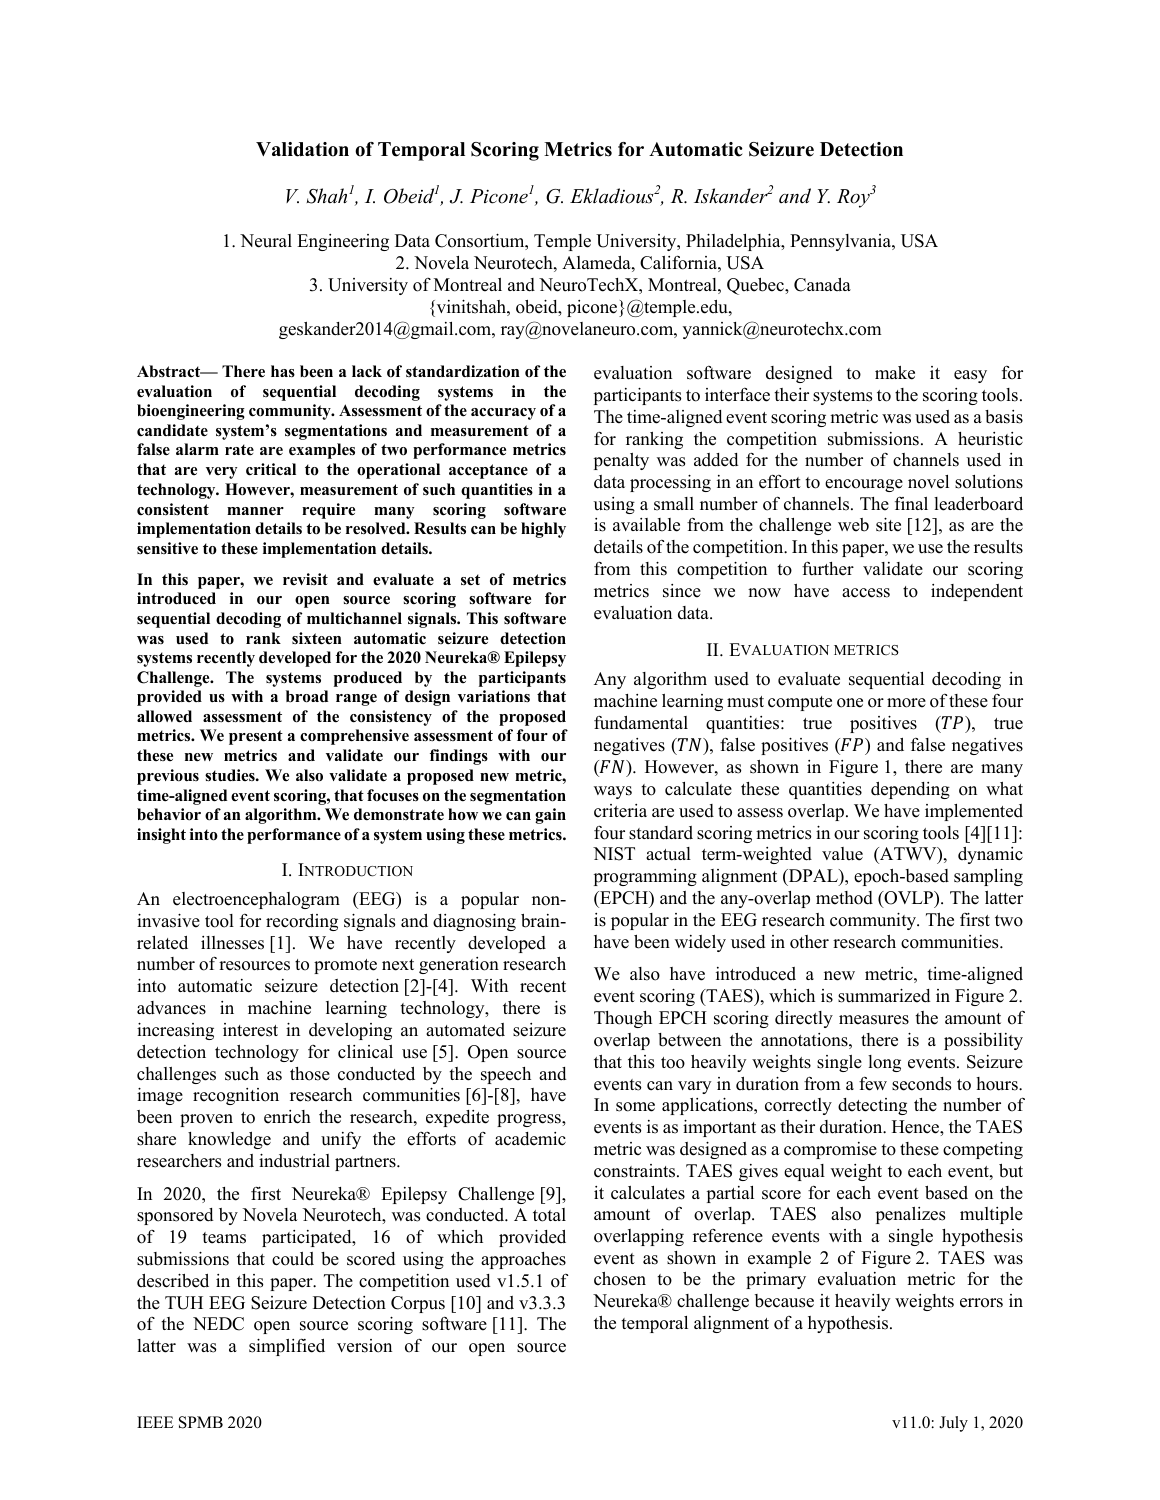
\includegraphics[width=\linewidth,height=46mm,keepaspectratio]{assets/history/neureka-scoring-first-page.png}\par\smallskip
      {\tiny Shah, Obeid, Picone, Ekladious, Iskander, Roy\newline IEEE SPMB 2020 scoring study\par}
  \end{columns}
  {\tiny\color{NTXMuted}Sources: \href{https://sccn.ucsd.edu/pipermail/eeglablist/2020/014884.html}{Yannick's challenge announcement}; \href{https://isip.piconepress.com/conferences/ieee_spmb/2020/papers/l02_05.pdf}{Validation of Temporal Scoring Metrics for Automatic Seizure Detection}\par}
  \note{[41:15--42:45] NeuroTechX and Novela Neurotech launched the challenge in 2020. The subsequent scoring paper lists Vinit Shah, Iyad Obeid, Joseph Picone, Georges Ekladious, Ray Iskander, and Yannick Roy; its affiliations link Temple's NEDC, Novela, and NeuroTechX. It reports 19 participating teams and 16 scorable systems using TUH EEG Seizure Detection Corpus v1.5.1 and NEDC scoring software v3.3.3. Say seizure detection, not prospective seizure prediction or diagnosis. The example belongs in the broader EEG machine-learning story: the challenge was not restricted to deep neural networks. Patient-separated train/development/evaluation sets and sensitivity to scoring choices illustrate why shared data need shared evaluation. No claim of approved clinical deployment, open patient-data redistribution, or exclusive NTX authorship of TUH.}
\end{frame}

% Existing benchmark, toolkit, methods-community and foundation-challenge frames follow.
\begin{frame}{Braindecode: deep learning joins the shared toolkit}
  \begin{columns}[c,onlytextwidth]
    \column{.45\textwidth}
      \small
      \NTXPoint{2017: deep learning for EEG}{Schirrmeister et al.: ConvNets and open-source Braindecode.}
      \NTXPoint{A connected research toolkit}{PyTorch, MNE, MOABB datasets, and pretrained models.}
      \NTXPoint{From classical baselines to learned features}{Train neural decoders within a reproducible EEG workflow.}
    \column{.51\textwidth}
      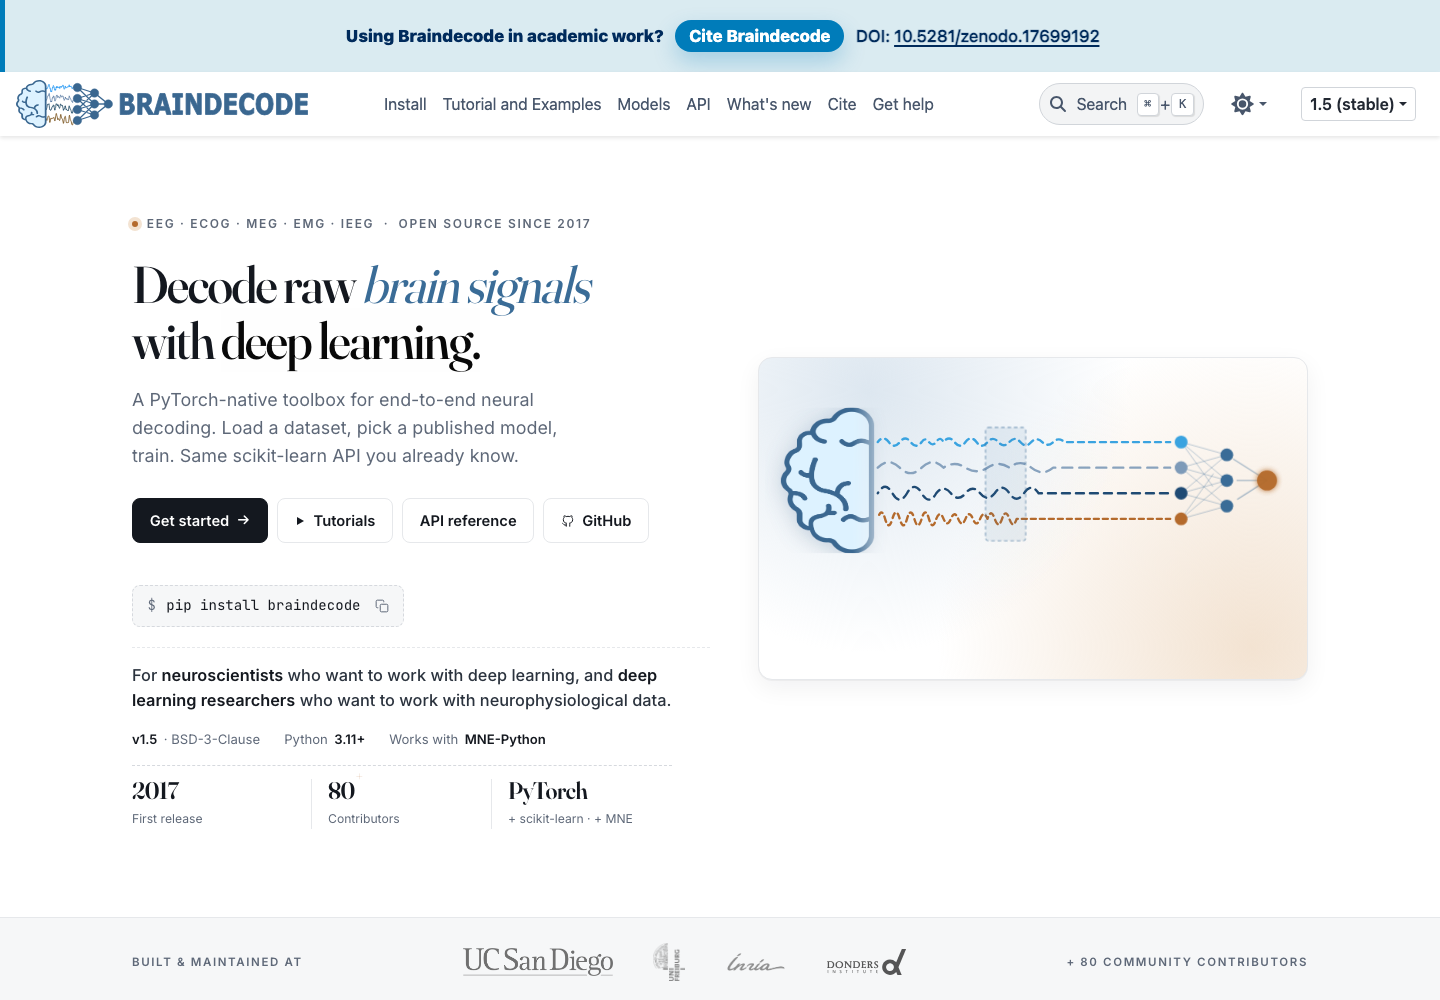
\includegraphics[width=\linewidth,height=45mm,keepaspectratio]{assets/history/braindecode-homepage.png}
      \par\smallskip{\scriptsize Braindecode's official project homepage\par}
  \end{columns}
  {\tiny\color{NTXMuted}Sources: \href{https://doi.org/10.1002/hbm.23730}{Schirrmeister et al., 2017}; \href{https://braindecode.org/stable/}{Braindecode}; \href{https://github.com/braindecode/OpenEEGBench}{Guetschel et al., OpenEEG-Bench, 2026}\par}
  \note{[42:45--44:15] Braindecode's foundational paper is Schirrmeister et al., Deep learning with convolutional neural networks for EEG decoding and visualization, Human Brain Mapping 2017, doi:10.1002/hbm.23730. Current documentation describes PyTorch/MNE integration and access to MOABB and pretrained models. OpenEEG-Bench is a distinct benchmark under the Braindecode organization, not a renamed MOABB or the NeurIPS competition itself. Guetschel, Aristimunha, Truong, Kokate, Tangermann, and Delorme's Toward OpenEEG-Bench paper builds explicitly on organizing the NeurIPS 2025 EEG Foundation Model Challenge. Its initial study covers five models and ten datasets. The current repository lists twelve datasets and probing, parameter-efficient adaptation, and full fine-tuning options. Do not mix those scopes or give an unverified current leaderboard ranking. Community contribution here means testing models under comparable preprocessing, splits, and adaptation procedures; not claiming NTX owns these projects.}
\end{frame}


\begin{frame}{OpenEEG-Bench: how should we adapt foundation models?}
  \begin{columns}[c,onlytextwidth]
    \column{.49\textwidth}
      \small
      \NTXPoint{A community-driven benchmark}{Compare EEG foundation models with shared data and evaluation pipelines.}
      \NTXPoint{Adaptation is part of the question}{Frozen-encoder probes, parameter-efficient adaptation, and full fine-tuning are different tests.}
      \NTXPoint{A contribution chapters can make}{Reproduce baselines, test new datasets, and report both accuracy and training cost.}
    \column{.47\textwidth}
      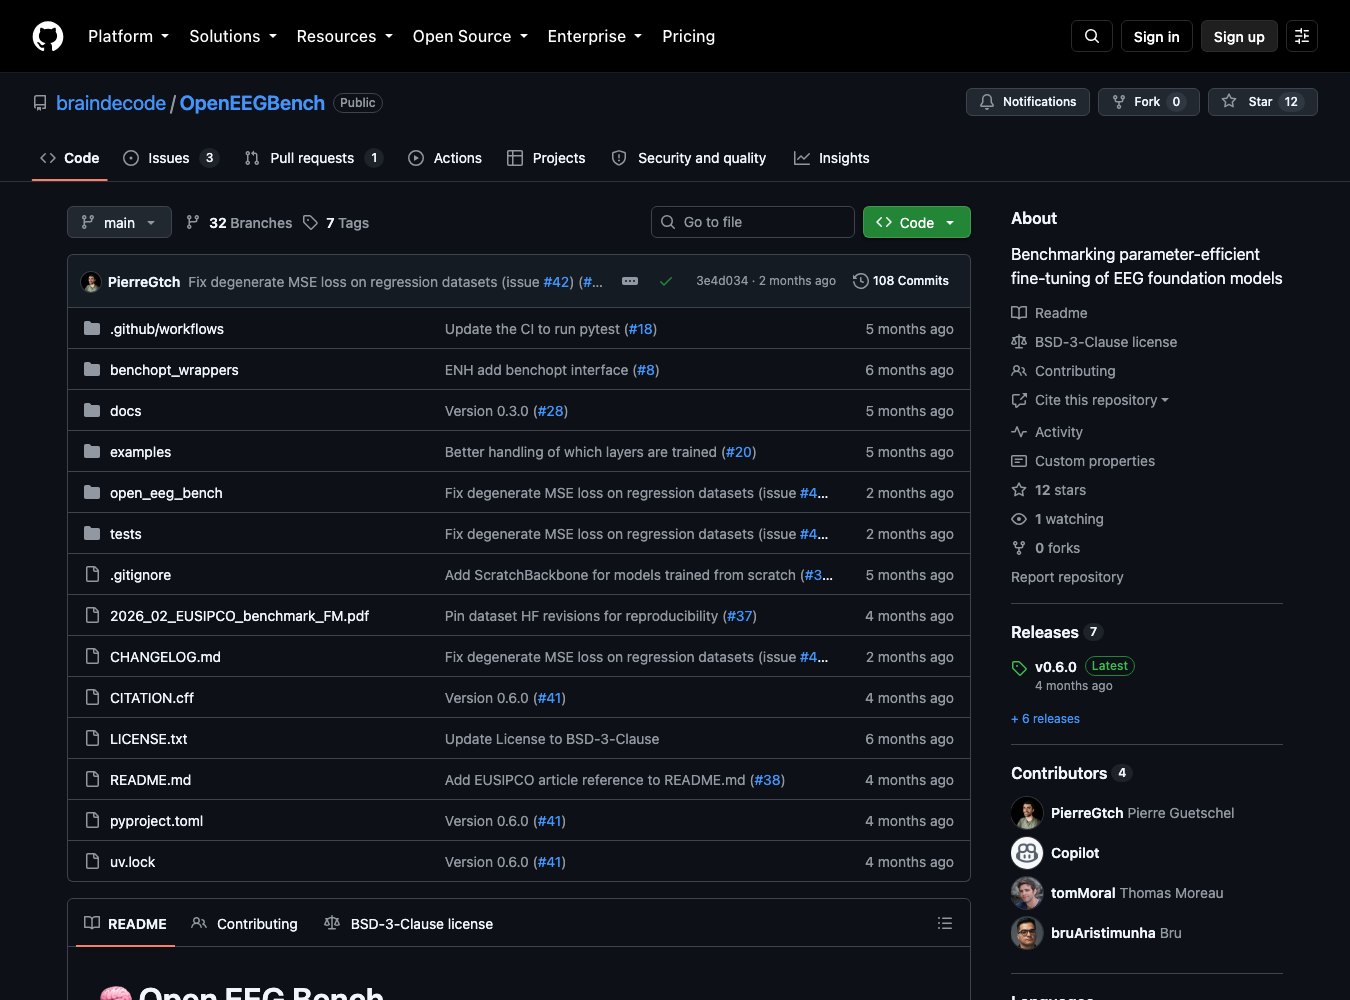
\includegraphics[width=\linewidth,height=43mm,keepaspectratio]{assets/history/openeegbench-repository.png}\par\smallskip
      {\tiny OpenEEG-Bench / Braindecode GitHub organization\par}
  \end{columns}
  \NTXSource{https://github.com/braindecode/OpenEEGBench}{Guetschel and colleagues, OpenEEG-Bench, 2026}
  \note{[44:15--45:45] This dedicated slide separates the benchmark from the Braindecode software history. The initial Toward OpenEEG-Bench paper evaluated five models on ten datasets; the evolving repository has a different scope. Avoid presenting either number as a permanent total. The current code supports frozen encoders, ridge probes, low-rank and other parameter-efficient approaches, full fine-tuning and two-stage adaptation. These answer different questions and must not be pooled into an undifferentiated leaderboard. Community contribution is our proposed use of the project, not a claim of NTX ownership or an established chapter program.}
\end{frame}

\begin{frame}{NeuroAtlas: a reality check for EEG foundation models}
  \begin{columns}[c,onlytextwidth]
    \column{.57\textwidth}
      \small
      \NTXPoint{KU Leuven + MIT, 2026}{42 datasets; approximately 260,000 hours across epilepsy, sleep, brain age, and BCI.}
      \NTXPoint{What transfers from a frozen model?}{EEG foundation models, generic time-series foundation models, and supervised-pretrained baselines.}
      \NTXPoint{No consistent EEG-specific advantage}{Rankings vary across datasets and metrics; an out-of-the-box universal EEG model remains a goal.}
    \column{.39\textwidth}
      \centering
      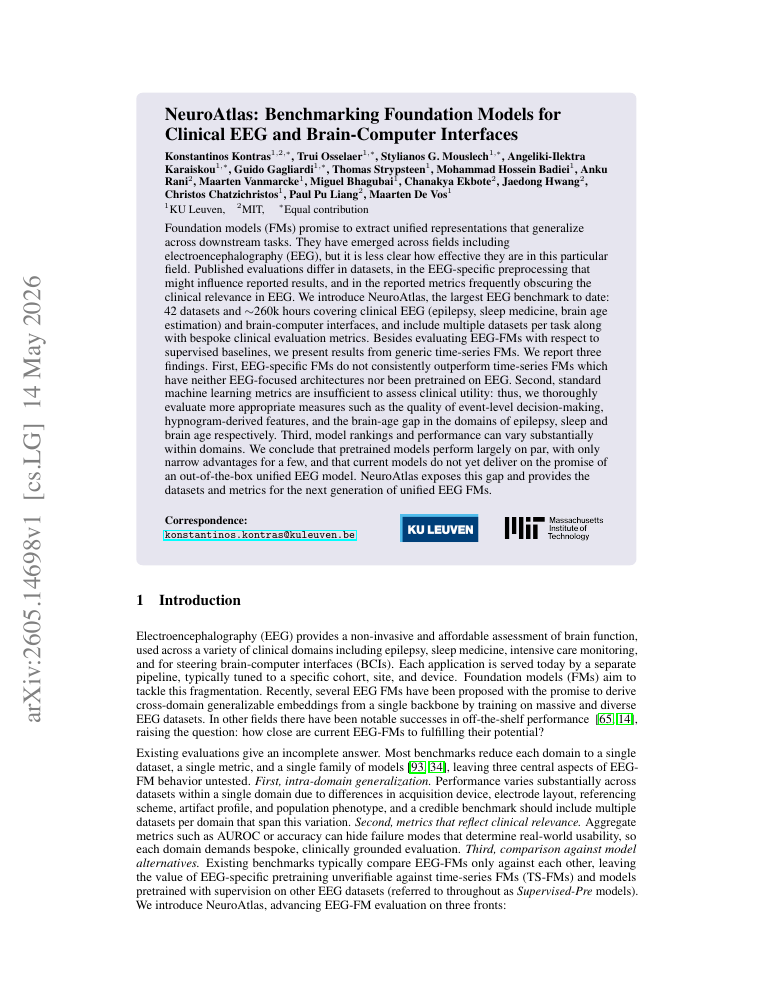
\includegraphics[width=\linewidth,height=46mm,keepaspectratio]{assets/history/neuroatlas-first-page.png}\par\smallskip
      {\tiny Kontras and colleagues, May 2026 preprint\par}
  \end{columns}
  \NTXSource{https://arxiv.org/abs/2605.14698}{NeuroAtlas: Benchmarking Foundation Models for Clinical EEG and Brain-Computer Interfaces}
  \note{[45:45--47:15] NeuroAtlas is the MIT/KU Leuven project Morgan confirmed, not NeuroSTORM. Its frozen-encoder protocol fits downstream probes rather than fully fine-tuning each backbone. The comparison includes supervised-pretrained neural models, not just classical non-neural pipelines. EEG-specific pretraining did not consistently beat generic time-series pretraining. Clinical-task metrics can change conclusions drawn from standard accuracy scores. This is a May 2026 preprint and a scoped benchmark, not proof that all foundation models fail or that any model is clinically ready.}
\end{frame}

\begin{frame}{Do NeuroFMs beat classical methods?}
  \begin{columns}[c,onlytextwidth]
    \column{.54\textwidth}
      \small
      \NTXPoint{Not consistently}{With scarce BCI data, gains over compact networks or classical decoders are often not significant.}
      \NTXPoint{Fine-tuning can change the result}{Data-rich settings can favor fine-tuned models. Frozen probing is a different test.}
      \NTXPoint{Keep the classical baseline}{Compare on the same task and splits, with uncertainty, calibration needs, and compute cost.}
    \column{.42\textwidth}
      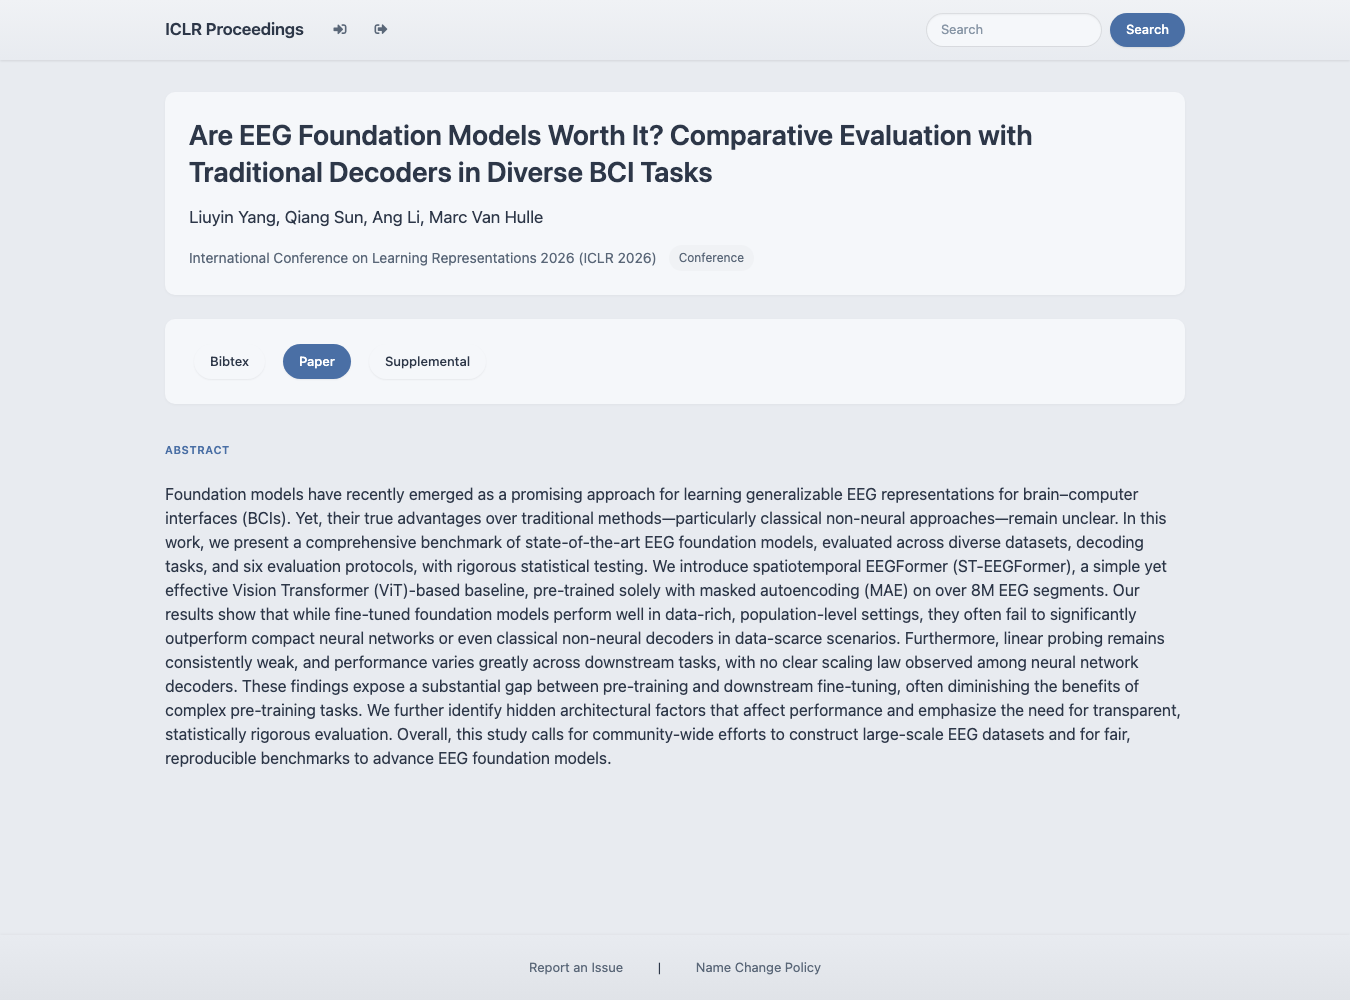
\includegraphics[width=\linewidth,height=43mm,keepaspectratio]{assets/history/eeg-fms-worth-it-page.png}\par\smallskip
      {\tiny Yang, Sun, Li, Van Hulle / ICLR 2026\newline Official proceedings abstract page\par}
  \end{columns}
  {\tiny\color{NTXMuted}Sources: \href{https://proceedings.iclr.cc/paper_files/paper/2026/hash/f0f39b7686634fc81ca0112566b2c05f-Abstract-Conference.html}{Are EEG Foundation Models Worth It?}; \href{https://github.com/LiuyinYang1101/STEEGFormer}{code and benchmark}\par}
  \note{[47:15--48:45] This separate ICLR 2026 study directly compares foundation models with traditional BCI decoders across six evaluation protocols. It supports a conditional answer, not a blanket claim that classical methods win. The authors report stronger foundation-model results with full fine-tuning and sufficient data, but frequently no significant advantage in data-scarce settings. Compact neural networks are distinct from classical non-neural methods. These experiments and NeuroAtlas have different protocols and cannot be merged into a single ranking. Our takeaway is to move into deep learning without discarding rigorous classical baselines. Cost and calibration reporting are our evaluation recommendations, not numerical results asserted from this paper.}
\end{frame}

\begin{frame}{CuttingGardens: global methods, local communities}
  \begin{columns}[c,onlytextwidth]
    \column{.55\textwidth}
      \small
      \NTXPoint{2023: the first distributed edition}{Shared M/EEG lectures; local tutorials, discussions, and networking.}
      \NTXPoint{2025: studying the conference model}{Published evaluation of ecological and social sustainability.}
      \NTXPoint{Next: 21--25 September 2026}{A broadcast global program with local activities around the world.}
    \column{.41\textwidth}
      \centering
      
\includegraphics[width=\linewidth,height=46mm,keepaspectratio]{assets/history/cuttinggardens-2026.png}
      \par\smallskip{\scriptsize Official 2026 event artwork\par}
  \end{columns}
  {\tiny\color{NTXMuted}Sources: \href{https://cuttinggardens2023.org/}{CuttingGardens 2023}; \href{https://doi.org/10.1371/journal.pstr.0000177}{Corneyllie et al., 2025}; \href{https://cuttingeeg.org/cuttinggardens2026/}{CuttingGardens 2026}\par}
  \note{[48:45--50:15] CuttingGardens is part of the CuttingEEG conference series, not an NTX event or a Braindecode project. The 2023 meeting introduced distributed local hubs connected by a common program. Corneyllie, Walters, Chaumon and colleagues published Doing conferences differently: A decentralised multi-hub approach for ecological and social sustainability in PLOS Sustainability and Transformation on June 23, 2025, doi:10.1371/journal.pstr.0000177. The paper reports 21 hubs, 730 in-person and 300 online attendees for 2023; these are retrospective figures, not 2026 forecasts. The upcoming global meeting is September 21--25, 2026. Local dates and activities vary. The 2026 site contains inconsistent hub/continent totals, so none are asserted. The connection to NTX is a model for distributed methods education and participation, not a formal partnership claim.}
\end{frame}

\begin{frame}{From global hackathons to foundation-model challenges}
  \begin{columns}[c,onlytextwidth]
    \column{.52\textwidth}
      \small
  \NTXPoint{Global hackathons}{A community coming together around shared technical challenges.}
  \NTXPoint{2025: EEG Foundation Challenge}{Cross-task and cross-subject decoding.\newline NeurIPS competition; results highlighted at SfN.}
  \NTXPoint{2026: EEG/EMG Foundation Challenge}{Four tracks testing generalization across brain and body signals.\newline Winners present at the NeurIPS Brain and Body workshop.}
    \column{.44\textwidth}
      \centering
      {\small\textbf{2025 EEG $\longrightarrow$ 2026 EEG / EMG}\par}\medskip
      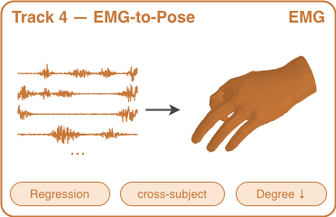
\includegraphics[width=\linewidth,height=33mm,keepaspectratio]{assets/history/challenge2026-emg-to-pose.png}\par\smallskip
      {\scriptsize A new brain-and-body task: EMG-to-pose\newline Official 2026 challenge illustration\par}
  \end{columns}
  {\tiny\color{NTXMuted}Sources: \href{https://eeg2025.github.io/}{EEG 2025}; \href{https://sccn.ucsd.edu/pipermail/eeglablist/2025/018754.html}{SCCN at SfN}; \href{https://neural-interfaces26.github.io/}{EEG/EMG 2026}; \href{https://brainbodyfm-workshop.github.io/}{Foundation Models for the Brain and Body}\par}
  \note{[50:15--51:45] Morgan describes this as a progression from the global hackathon community into larger research challenges. The 2025 competition was part of NeurIPS; SCCN's November 2025 SfN booth announcement invited discussion of its results. The 2026 challenge covers image retrieval from EEG, BCI decoding, sleep onset, and hand pose from EMG. Its website says winners will present at Foundation Models for the Brain and Body at NeurIPS. This is upcoming, not a completed event. The challenge site credits promotion via NeuroTechX, EEGLAB, and MNE-Python. Distinguish Morgan's community-history account from formal event ownership; do not imply NTX exclusively organized all these programs.}
\end{frame}

\begin{frame}{Toward a MindEye-style EEG reconstruction project}
  \begin{columns}[c,onlytextwidth]
    \column{.48\textwidth}
      \small
      \NTXPoint{Alljoined: public data + model code}{Alljoined-1.6M: 1.6M+ EEG-image trials, 20 participants. ENIGMA: EEG-to-image reconstruction.}
      \NTXPoint{An ambitious chapter project}{Reproduce the results, then work toward a live EEG-to-image demonstration.}
      \NTXPoint{A direction, not yet equivalence}{MindEye's real-time demonstration uses fMRI. ENIGMA's reported EEG results average repeated trials.}
    \column{.48\textwidth}
      \includegraphics[page=6,trim=52 340 65 80,clip,width=\linewidth,height=43mm,keepaspectratio]{assets/history/enigma-2026.pdf}\par\smallskip
      {\tiny ENIGMA, Fig. 3: authors' selected best-scoring outputs\newline Seen images, not imagined scenes\par}
  \end{columns}
  {\tiny\color{NTXMuted}Sources: \href{https://huggingface.co/datasets/Alljoined/Alljoined-1.6M}{Dataset (CC BY-NC-SA 4.0)}; \href{https://github.com/Alljoined/ENIGMA}{ENIGMA code}; \href{https://arxiv.org/abs/2602.10361}{Kneeland et al., 2026}; \href{https://arxiv.org/abs/2607.22753}{Real-time MindEye2 adaptation, 2026}\par}
  \note{[51:45--53:15] This is Morgan's proposed direction for ambitious community projects, not an announcement of an NTX deployment or a demonstrated EEG port of MindEye. Alljoined publicly provides a large consumer-hardware EEG-image dataset and ENIGMA training, inference, and evaluation code. Public availability does not imply unrestricted commercial reuse: the dataset card specifies CC BY-NC-SA 4.0. We have not verified a pretrained checkpoint release. ENIGMA reconstructs viewed stimuli using a shared EEG encoder and generative image model. Appendix A.1 reports averaging 80 repetitions per inference sample; Figure 3 selects the highest-scoring sampled outputs. These are not typical single-trial live results or literal readouts of imagination. Iyer and colleagues' July 2026 real-time MindEye2 adaptation uses fMRI and RT-Cloud. The opportunity is to reproduce EEG baselines, test held-out images and people, and measure end-to-end latency and single-trial performance before calling a system real-time.}
\end{frame}


\section{How do we add to the community?}

\begin{frame}{The NeuroTech Microcredential Program}
  \begin{columns}[T,onlytextwidth]
    \column{.62\textwidth}
      \NTXPoint{2022: partnership announced}{Queen's Centre for Neuroscience Studies and NeuroTechX; Ontario-funded development.}
      \NTXPoint{2024--2025: hands-on capstones}{First cohort: May 2024. Second: August 2025.\newline 15 students in each cohort.}
      \NTXPoint{Online learning into lab practice}{Neuroscience, recording, imaging, and ethics;\newline a two-week, team-based capstone.}
    \column{.33\textwidth}
      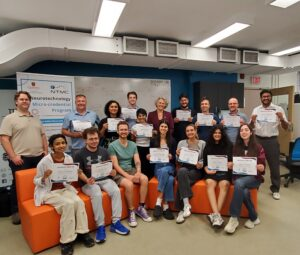
\includegraphics[width=\linewidth]{assets/history/queens-capstone-2025.jpg}
      \par\smallskip{\scriptsize 2025 capstone cohort\par}
  \end{columns}
  {\tiny\color{NTXMuted}Sources: \href{https://www.queensu.ca/gazette/media/news-release-queen-s-micro-credentials-address-knowledge-gaps-burgeoning-neurotech-industry}{Queen's launch announcement, October 2022}; \href{https://neurotechmicrocreds.com/capstone/}{program history and cohort photo}\par}
  \note{[53:15--55:15] Queen's announced the partnership on October 17, 2022, with Susan Boehnke directing the program. Its announcement anticipated online courses from January 2023; that is an announced schedule, not independently verified delivery. The program documents 15 students in each of its first two capstones, May 2024 and August 2025. Students combined workshops with project design, data collection, analysis, and presentations. The current homepage describes an initial NTX partnership; do not infer present governance. The photographed cohort is 2025. This is the concrete education history that sets up more ambitious future student projects.}
\end{frame}

\section{The Second Wave of BCI}
\NTXDivider{The Second Wave of BCI}

\begin{frame}{Brain implants did not begin with Neuralink}
  \begin{columns}[c,onlytextwidth]
    \column{.55\textwidth}
      \small
      \NTXPoint{A longer implant history}{From cardiac pacemakers to cochlear implants and deep brain stimulation.}
      \NTXPoint{Different interfaces and purposes}{Cochlear implants stimulate the auditory nerve; DBS stimulates brain targets. Neither is synonymous with a motor BCI.}
      \NTXPoint{BCI before the headlines}{Utah arrays and BrainGate preceded Neuralink. Hochberg et al. (2006): implanted neural control of devices by a person with tetraplegia.}
    \column{.41\textwidth}
      \centering
      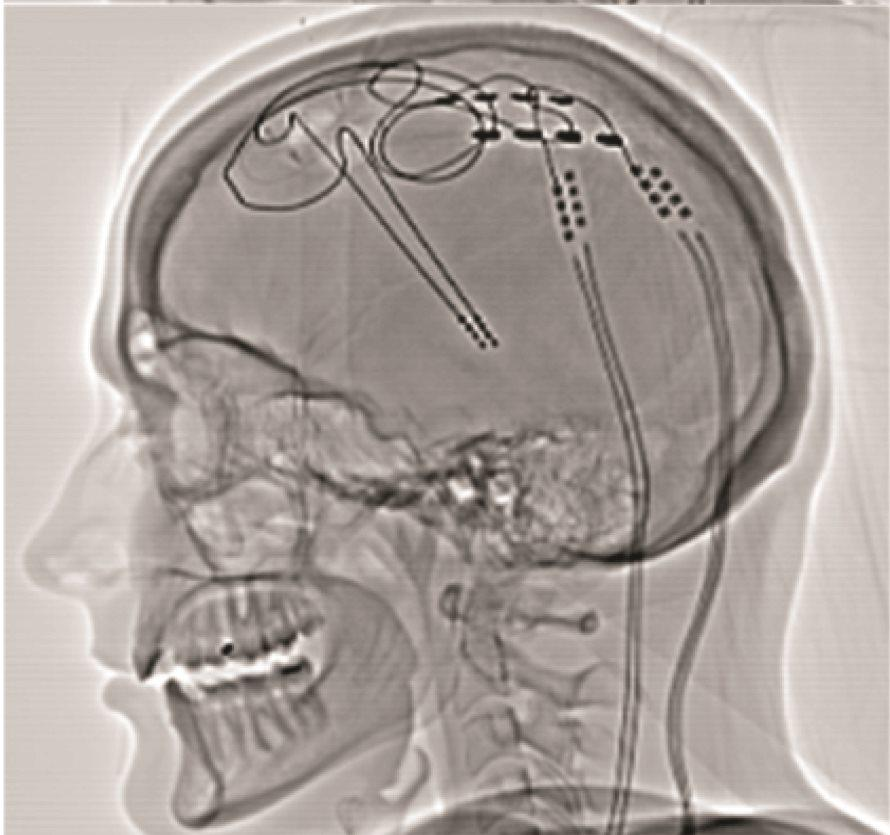
\includegraphics[width=\linewidth,height=43mm,keepaspectratio]{assets/history/india-implant-xray-000.jpg}\par\smallskip
      {\tiny Implant image reused from my NeuroTechX India talk\newline Original slide credit: Ingenia\par}
  \end{columns}
  {\tiny\color{NTXMuted}Sources: \href{https://www.nidcd.nih.gov/health/cochlear-implants}{NIDCD}; \href{https://www.ninds.nih.gov/health-information/disorders/deep-brain-stimulation-dbs}{NINDS}; \href{https://doi.org/10.1038/nature04970}{Hochberg et al., Nature, 2006}\par}
  \note{[55:15--56:45] Adapted from slides 5--18 of Morgan's NeuroTechX India presentation, Neuralink and Brain-Computer Interfaces. Begin with the implant history, not a claim that these devices are all BCIs. Cardiac pacemakers are an engineering antecedent, not brain implants. Cochlear implants act on the auditory nerve, whereas DBS electrodes deliver stimulation in brain targets. The image is carried over from slide 6, which credits Ingenia; do not identify it as a Neuralink device or infer a patient diagnosis or exact implant model. BrainGate's 2006 paper provides a concrete human intracortical BCI milestone, not the beginning of the whole field. Omit the old deck's sweeping clinical claims, device comparisons, and relative dates.}
\end{frame}

\begin{frame}{The second wave: BCI enters the public imagination}
  \begin{columns}[c,onlytextwidth]
    \column{.53\textwidth}
      \small
      \NTXPoint{My framing: a second wave}{Elon Musk and Neuralink's marketing brought BCI into a much wider public conversation.}
      \NTXPoint{Engineering and publicity are different}{Neuralink's 2019 paper described flexible threads, insertion robotics, and custom electronics. Public attention is not clinical evidence.}
      \NTXPoint{The community opportunity}{Turn that curiosity into learning, open projects, and informed founders --- while keeping expectations grounded.}
    \column{.43\textwidth}
      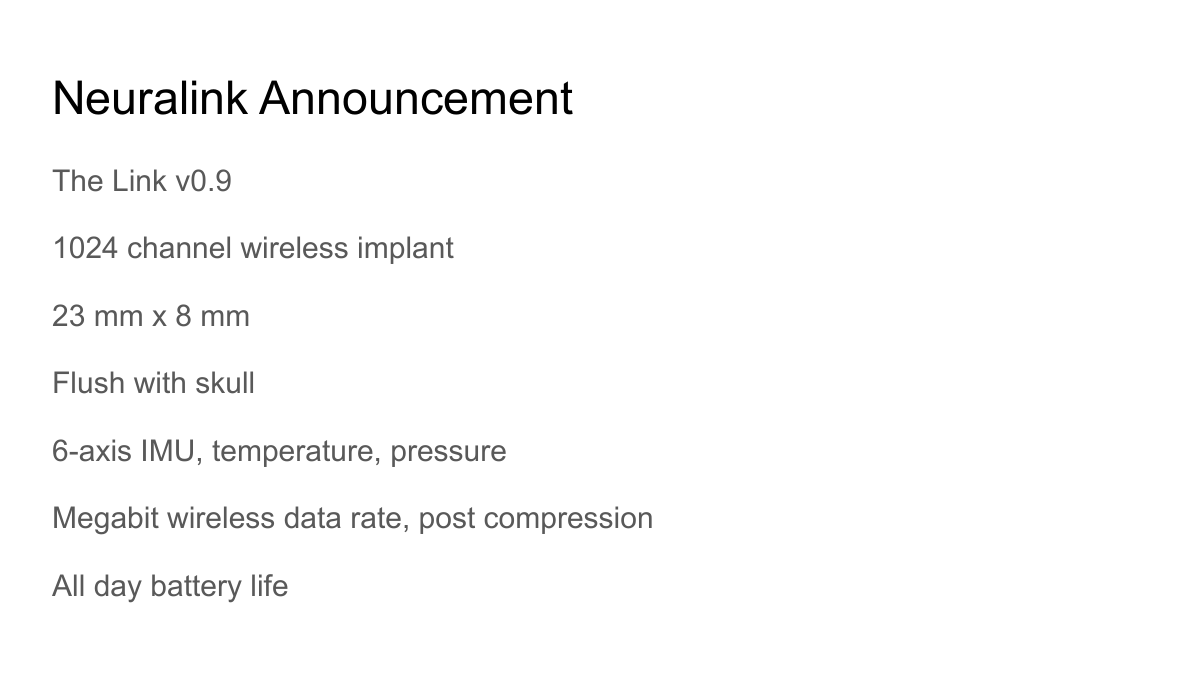
\includegraphics[width=\linewidth,height=40mm,keepaspectratio]{assets/history/india-neuralink-announcement-historical.png}\par\smallskip
      {\scriptsize From my NeuroTechX India presentation\par}
      {\tiny Historical Link v0.9 announcement slide\newline Not current specifications or verified clinical outcomes\par}
  \end{columns}
  {\tiny\color{NTXMuted}Sources: \href{https://docs.google.com/presentation/d/1tg9bppwmBDEhUSRyLswBP6Aj8QDDXgv3TXCEmOl_0yQ/edit}{Morgan Hough, NeuroTechX India deck}; \href{https://doi.org/10.2196/16194}{Musk \& Neuralink, JMIR, 2019}. ``Second wave'': Morgan's interpretation.\par}
  \note{[56:45--58:15] This is Morgan's proposed second-wave narrative, not a standard historical taxonomy or a claim that Neuralink invented BCI. The original India deck discussed Link v0.9 announcements alongside predecessors and competitors. The inset is an archival reproduction of slide 18, not an endorsement of its announcement claims as measured performance. Do not read its numbers as current product specifications. Distinguish the 2019 research platform in the cited paper from the later Link v0.9 announcement. The marketing/public-awareness argument is Morgan's interpretation; no quantitative attribution of investment or recruitment is asserted. Connect this discussion back to NeuroTechX: attention can bring people through the door, but learning, collaboration, and evidence help them become contributors and founders.}
\end{frame}

\begin{frame}{InterfaceNeuro: bringing the implant ecosystem together}
  \begin{columns}[c,onlytextwidth]
    \column{.52\textwidth}
      \small
      \NTXPoint{From InterfaceRice to InterfaceNeuro}{A joint Rice--Georgia Tech meeting series connecting research, engineering, medicine, and industry.}
      \NTXPoint{2025: Georgia Tech, May 7--8}{Brain, body, and machine interfaces; \emph{Wired Lives} brought implanted-BCI users' stories into the conversation.}
      \NTXPoint{2026: Rice, May 19--20}{Translational brain research, chronic BCI implants, and the wider social context.}
    \column{.44\textwidth}
      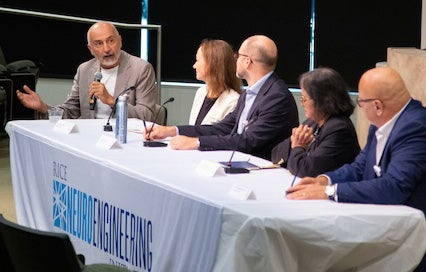
\includegraphics[width=\linewidth,height=40mm,keepaspectratio]{assets/history/interfaceneuro-rice-2026.jpg}\par\smallskip
      {\tiny InterfaceNeuro 2026, Rice University\newline Photo: Donald Soward / Rice University\par}
  \end{columns}
  {\tiny\color{NTXMuted}Sources: \href{https://inc.rice.edu/about}{Conference history}; \href{https://inc.rice.edu/}{InterfaceNeuro}; \href{https://news.rice.edu/news/2026/rice-hosts-translational-brain-research-conference}{Rice 2026 report / photo}\par}
  \note{[58:15--59:45] InterfaceNeuro and the Rice/Georgia Tech meetings are a connected series, not three independent conferences. The official history documents InterfaceRice in 2024, InterfaceNeuro at Georgia Tech on May 7--8, 2025, and the 2026 Rice event on May 19--20. The history page's odd/even-year description contradicts those dated events; use the actual dates, not that rule. The 2025 Story Collider event Wired Lives included people living with implanted BCIs. Rice's 2026 recap confirms multidisciplinary participation and credits Donald Soward for this panel photo. These meetings illustrate where sustained dialogue follows public interest in implants; no NTX ownership, partnership, or Morgan attendance is inferred.}
\end{frame}

\begin{frame}{Follow the methods communities: Lead-DBS and NEURAL}
  \begin{columns}[c,onlytextwidth]
    \column{.55\textwidth}
      \small
      \NTXPoint{Lead-DBS: recurring participation}{Developer meetings, workshops, shared code, and support around DBS imaging and analysis.}
      \NTXPoint{Bordeaux: learning the disconnectome}{NEURAL workshops with Michel Thiebaut de Schotten and colleagues; 2025 and June 8--12, 2026.}
      \NTXPoint{Stay connected beyond the headlines}{Follow the meetings, learn the tools, and contribute to the communities doing the methodological work.}
    \column{.41\textwidth}
      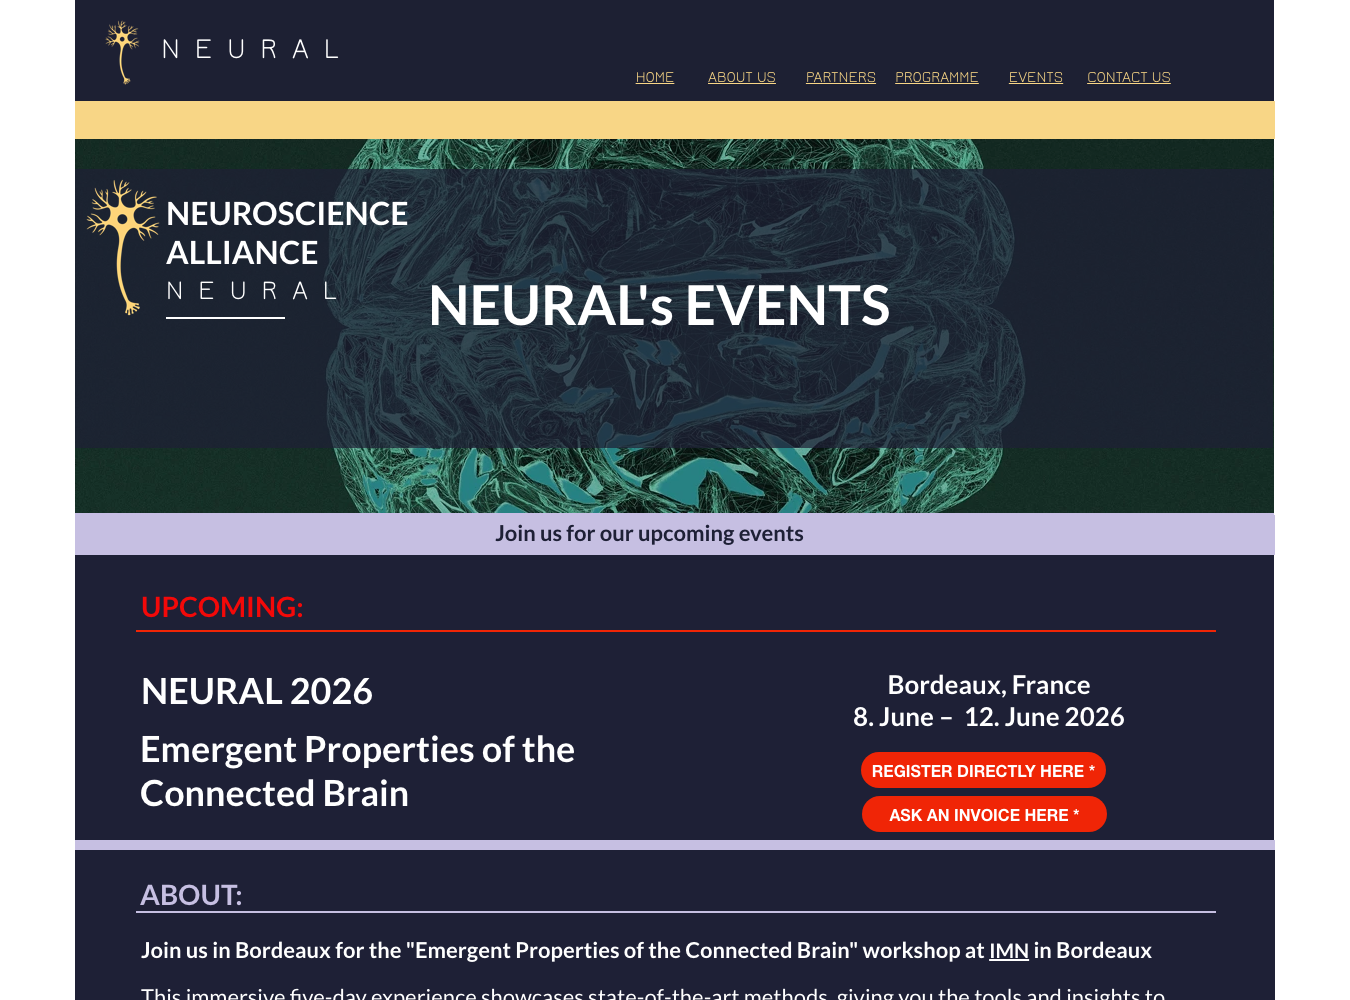
\includegraphics[width=\linewidth,height=43mm,keepaspectratio]{assets/history/neural-bordeaux-2026-page.png}\par\smallskip
      {\tiny NEURAL: Emergent Properties of the Connected Brain\newline Official page; June 2026 event is now past\par}
  \end{columns}
  {\tiny\color{NTXMuted}Sources: \href{https://netstim.gitbook.io/leaddbs/ways-to-contribute-to-lead-dbs}{Lead-DBS community}; \href{https://www.lead-dbs.org/helpsupport/workshops/}{workshops}; \href{https://storage.googleapis.com/bcblabweb/events.html}{NEURAL program}\par}
  \note{[59:45--61:15] Lead-DBS's contributor guide invites people to monthly developer meetings coordinated on Slack; its workshop archive documents hands-on training. This is an imaging and analysis community, not an implanted motor-BCI product. The French meeting is identified here as NEURAL, Emergent Properties of the Connected Brain, in Bordeaux. Stephanie Forkel's institutional record documents the October 2025 edition; the organizer page lists June 8--12, 2026, with Michel Thiebaut de Schotten teaching the disconnectome, alongside Valentina Pacella, Stephanie Forkel and Anna Matsulevits. Its stale Upcoming label should not be repeated in a September talk. Disconnectome methods concern network disconnection, including after lesions; they are not synonymous with DBS targeting or BCI decoding. These are related communities to follow, not NTX programs or proof of clinical effectiveness.}
\end{frame}

% Open participation in analysis, not permission to perform implant procedures.
\begin{frame}{OpenScope: access to an observatory, not just a dataset}
  \begin{columns}[c,onlytextwidth]
    \column{.54\textwidth}
      \small
      \NTXPoint{Allen Institute's shared platform}{External researchers propose experiments using mouse Neuropixels recordings and two-photon imaging.}
      \NTXPoint{A 2026 release to work with}{Predictive Processing data: public S3 assets and partial NWB files; complete DANDI releases follow as finalized.}
      \NTXPoint{An entry point without your own implant lab}{Use the OpenScope Databook to analyze recordings and ask new questions.}
    \column{.42\textwidth}
      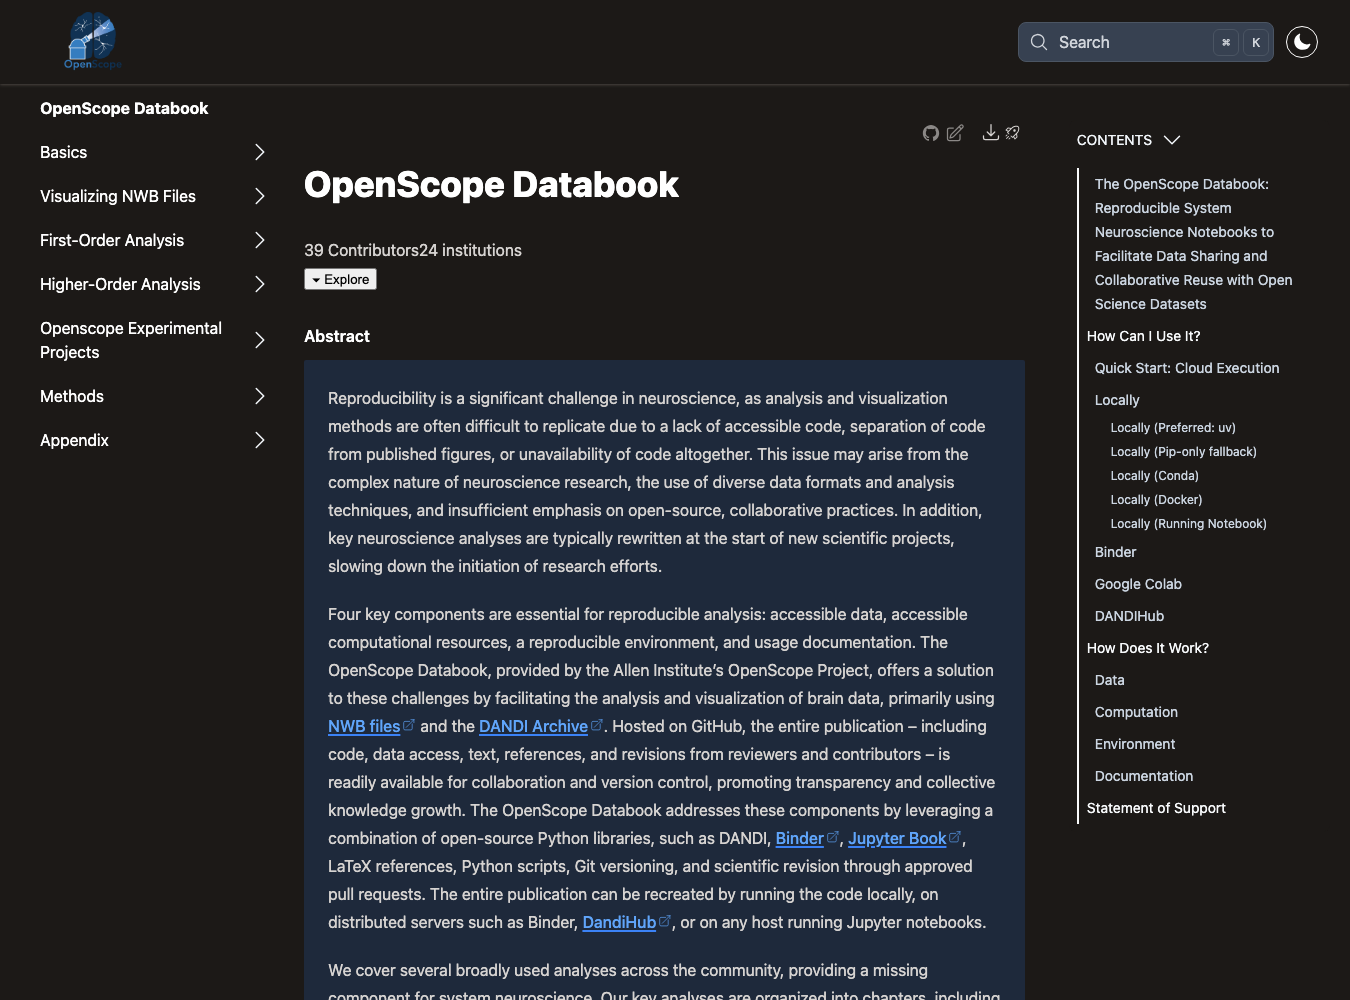
\includegraphics[width=\linewidth,height=43mm,keepaspectratio]{assets/history/openscope-databook-page.png}\par\smallskip
      {\tiny OpenScope Databook / Allen Institute\par}
  \end{columns}
  {\tiny\color{NTXMuted}Sources: \href{https://www.allenneuraldynamics.org/projects/openscope}{OpenScope}; \href{https://allenneuraldynamics.github.io/openscope-community-predictive-processing/data-access/}{2026 release guide}; \href{https://alleninstitute.github.io/openscope_databook/}{Databook}\par}
  \note{[61:15--62:45] OpenScope lowers the cost of experimental access through a selected-proposal model and makes recorded data reusable. It is primarily mouse systems neuroscience, not a human implant trial. Do not imply an application call is currently open: the program page notes no 2025 call and points to its community project. Its traditional release policy includes an embargo. The Predictive Processing guide specifically labels its release ongoing as of April 2026; complete multimodal NWB files on DANDI were still being finalized. Public S3 access needs no AWS account. We distinguish released assets from promised future completion. Reanalysis offers a way into invasive-recording methods without performing surgery or owning a recording facility.}
\end{frame}

\begin{frame}{DANDI + NWB: make invasive recordings reusable}
  \begin{columns}[c,onlytextwidth]
    \column{.53\textwidth}
      \small
      \NTXPoint{NWB is the shared data standard}{Recordings, experimental context, and metadata in a form supported by common tools.}
      \NTXPoint{DANDI is the archive}{Find datasets, inspect metadata, download or stream data, and cite the version used.}
      \NTXPoint{Access to analysis across laboratories}{Study neural signals and behavior without collecting every dataset yourself. Respect each dataset's terms.}
    \column{.43\textwidth}
      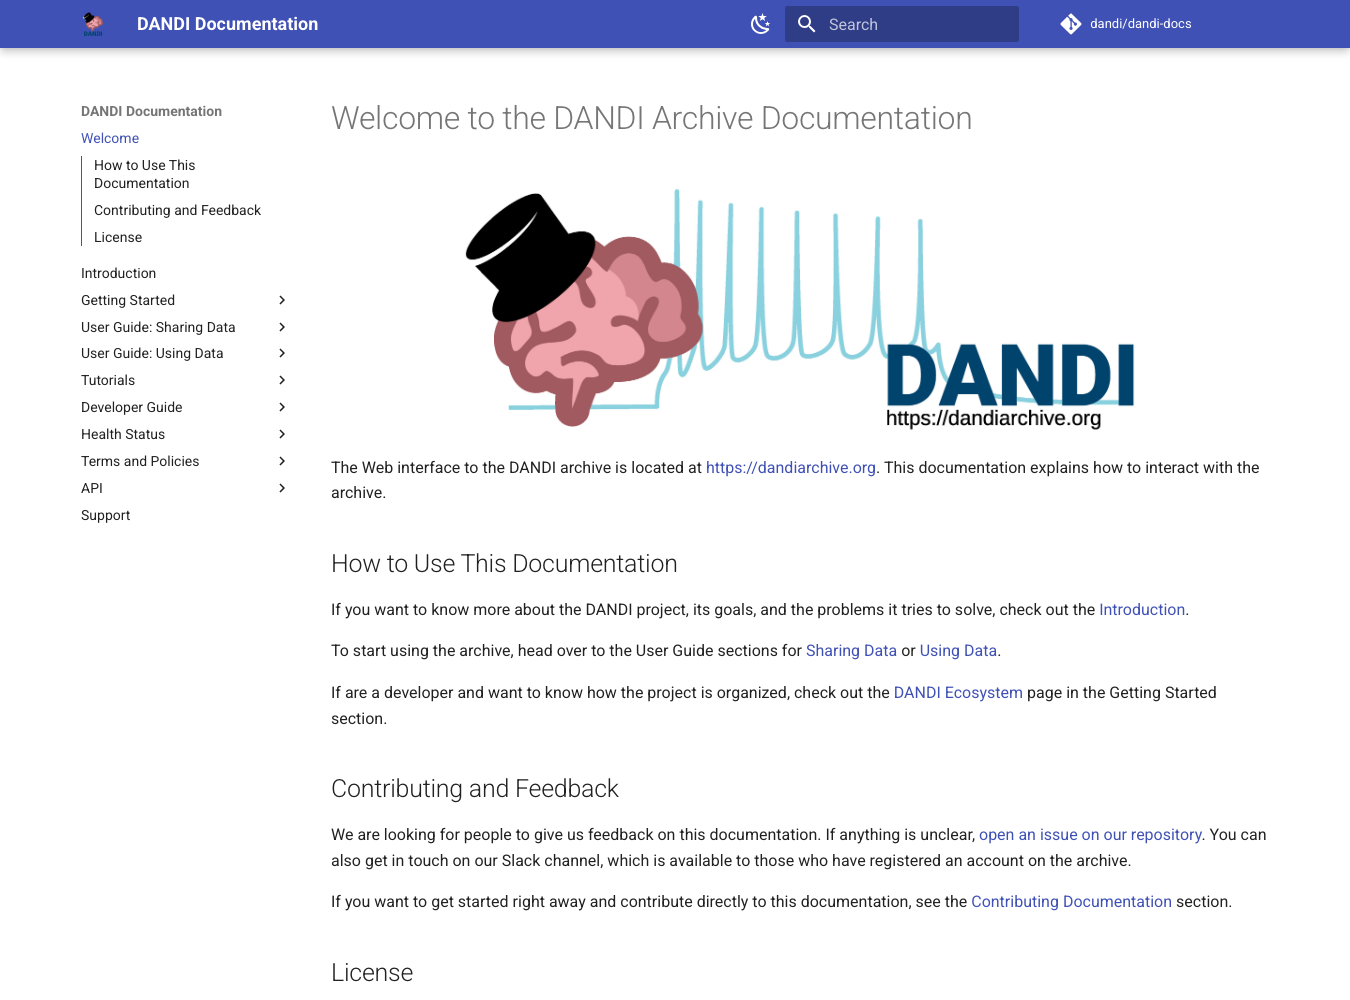
\includegraphics[width=\linewidth,height=43mm,keepaspectratio]{assets/history/dandi-documentation-page.png}\par\smallskip
      {\tiny Official DANDI archive documentation\par}
  \end{columns}
  {\tiny\color{NTXMuted}Sources: \href{https://docs.dandiarchive.org/}{DANDI documentation}; \href{https://nwb.org/}{Neurodata Without Borders}\par}
  \note{[62:45--64:15] Keep the roles clear: NWB is a neurophysiology data standard; DANDI provides discovery, storage, access and publication infrastructure. Neither is itself an implant or a clinical trial. The archive spans species and recording modalities, not exclusively human invasive BCI. Practical accessibility means fewer custom file readers, documented experimental context, and reusable analysis workflows. Streaming can reduce the need for full local downloads but does not eliminate bandwidth, compute or expertise requirements. Cite the precise Dandiset version and check its license and conditions; metadata availability does not mean all studies have identical access rules.}
\end{frame}

\begin{frame}{NeuroDataReHack 2026: learn by reusing real recordings}
  \begin{columns}[c,onlytextwidth]
    \column{.54\textwidth}
      \small
      \NTXPoint{July 12--17, HHMI Janelia}{A week of collaborative reanalysis in Ashburn, Virginia.}
      \NTXPoint{NWB + DANDI, with expert support}{OpenScope data, spike analysis, visualization, and independent projects; recorded talks are public.}
      \NTXPoint{Lower the participation barrier}{No registration fee; lodging and meals provided for participants. Travel remained their responsibility.}
    \column{.42\textwidth}
      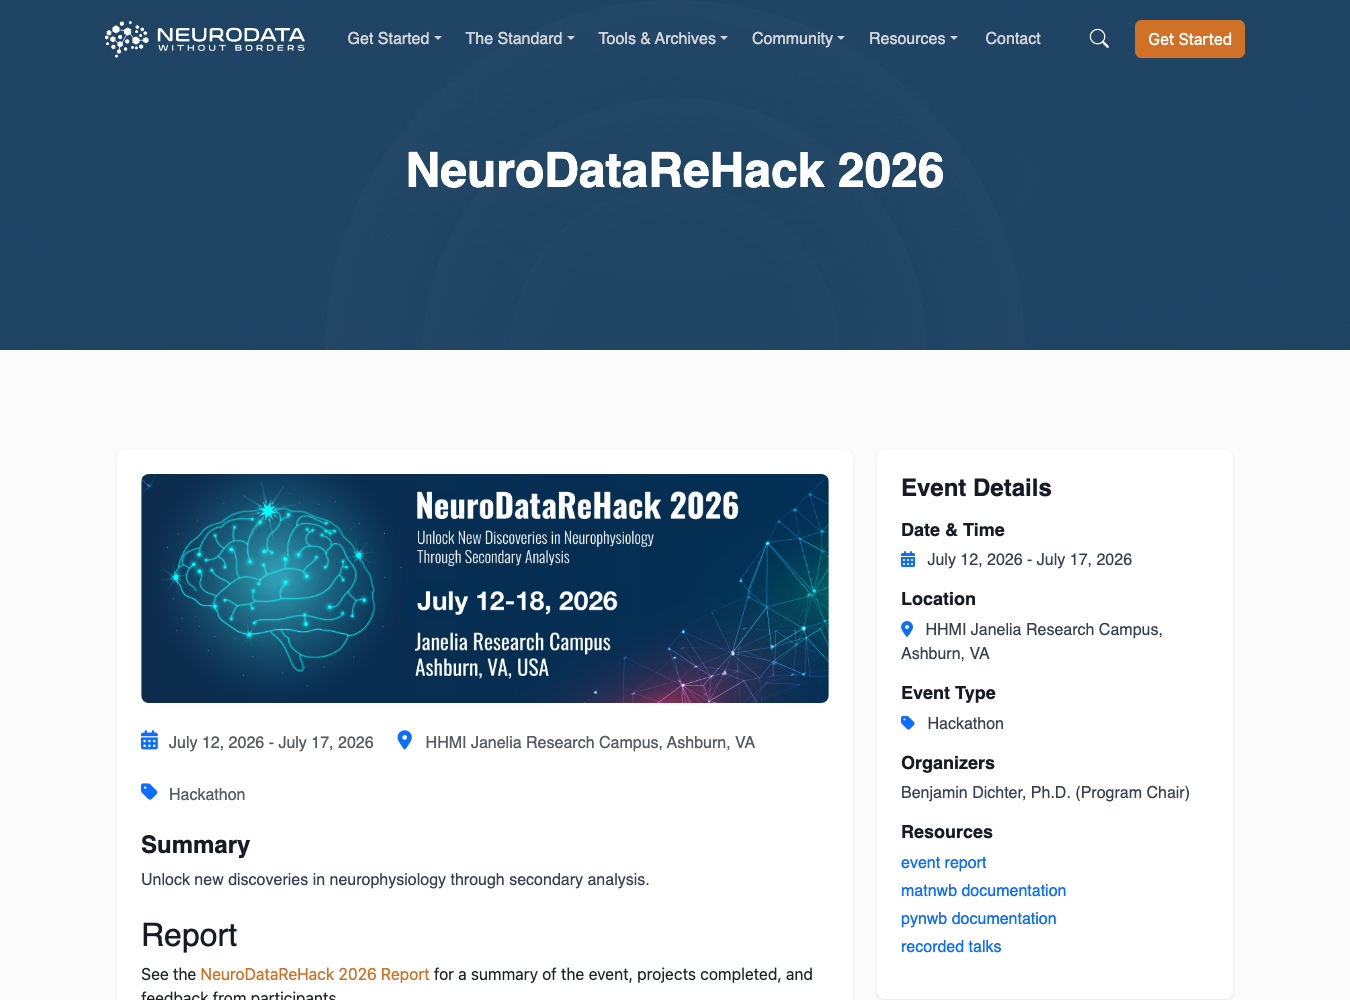
\includegraphics[width=\linewidth,height=43mm,keepaspectratio]{assets/history/neurodatarehack-2026-page.png}\par\smallskip
      {\tiny Official 2026 event page / NWB\par}
  \end{columns}
  \NTXSource{https://nwb.org/events/hck26-2026-janelia-ndrh/}{NeuroDataReHack 2026: program, report, and recordings}
  \note{[64:15--65:45] This summer's event has already happened; do not present registration as open. Its focus was secondary analysis rather than converting new data to NWB. Admission was selective and basic programming plus neurophysiology experience were expected, so free attendance does not mean unrestricted admission. Recorded teaching extends access beyond the cohort. These resources help people contribute computational work on invasive recordings while original data collection remains with qualified laboratories. No NTX organizing role is asserted.}
\end{frame}

\begin{frame}{Neuro Galaxy: from open recordings to shared models}
  \begin{columns}[c,onlytextwidth]
    \column{.54\textwidth}
      \small
      \NTXPoint{Tools for neural foundation models}{\texttt{torch\_brain}: data loading, training pipelines, and models across recordings.}
      \NTXPoint{Hands-on learning at Janelia ReHack}{Alexandre Andre's \emph{Applying Neural Foundation Models} tutorial used \texttt{torch\_brain}.}
      \NTXPoint{A project our community can take on}{Start with public recordings, reproduce a decoder, then test transfer across sessions or subjects.}
    \column{.42\textwidth}
      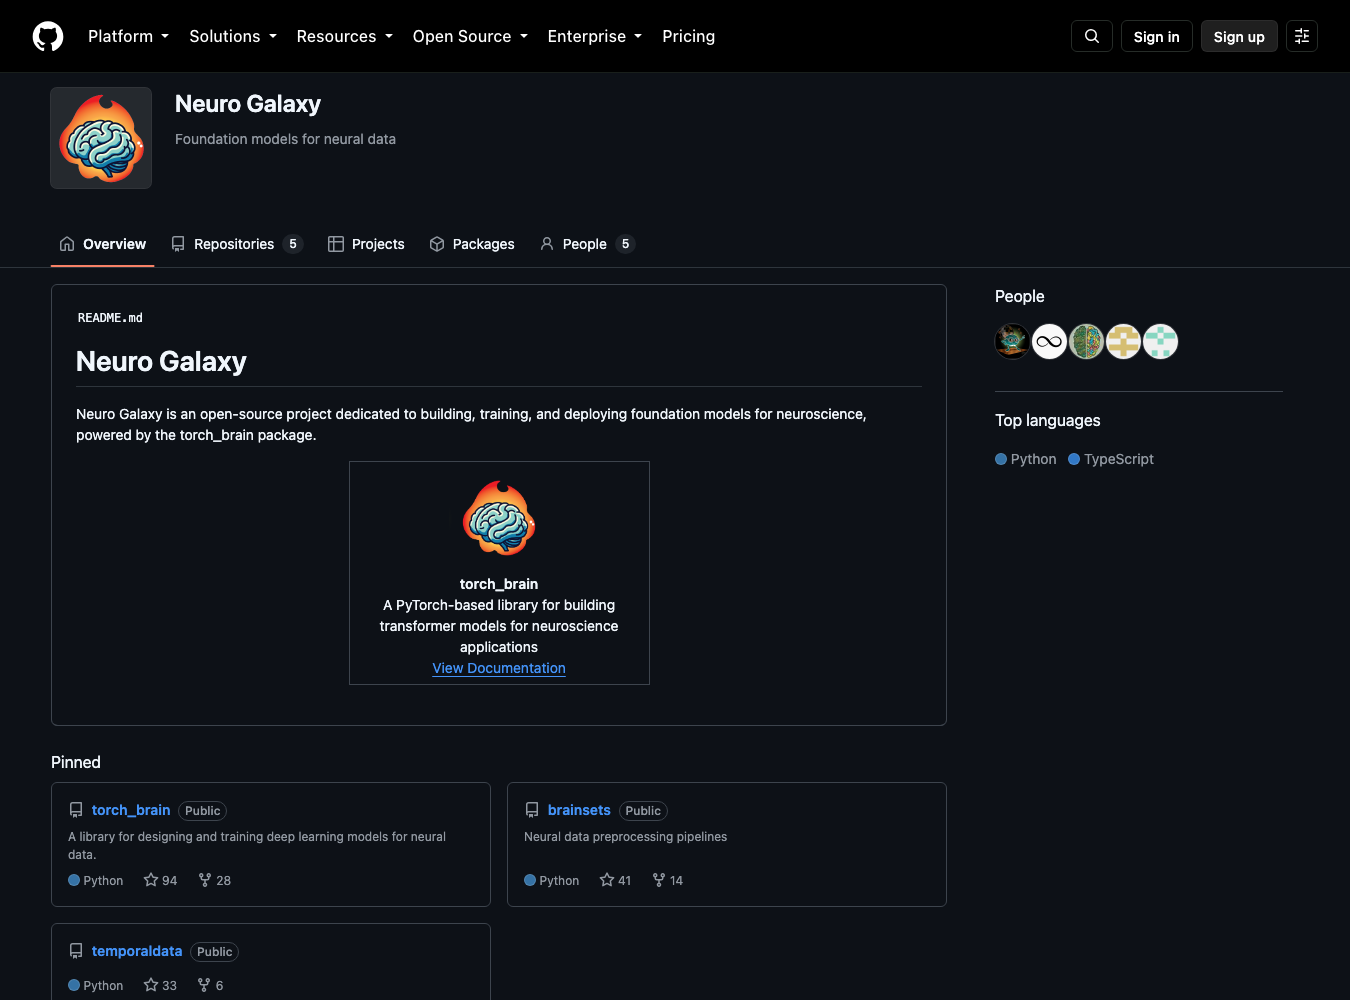
\includegraphics[width=\linewidth,height=43mm,keepaspectratio]{assets/history/neuro-galaxy-page.png}\par\smallskip
      {\tiny Neuro Galaxy / official GitHub organization\par}
  \end{columns}
  {\tiny\color{NTXMuted}Sources: \href{https://github.com/neuro-galaxy}{Neuro Galaxy}; \href{https://github.com/neuro-galaxy/torch_brain}{torch\_brain}; \href{https://nwb.org/events/hck26-2026-janelia-ndrh/}{ReHack 2026 program}\par}
  \note{[65:45--67:15] Neuro Galaxy provides an open-source framework, not one universal model or a commercial implant platform. The current torch\_brain repository says temporaldata and brainsets have been merged into it; pin versions when following older tutorials. Data loading supports neural and behavioral modalities, including spikes and regularly sampled signals. The verified event link is Alexandre Andre's July 14 Janelia tutorial. A separate NeuroGalaxy-branded hackathon has not yet been identified; do not invent its name, date or results. The proposed chapter project is Morgan's opportunity narrative, not an announced program. Retain classical baselines and held-out evaluation; access to code alone does not establish generalization or clinical readiness.}
\end{frame}


\section{What does the future hold for neurotech founders?}
\NTXDivider{The Next Neurotech Founders}
\begin{frame}{McGill NeuroTech: student-built TMS research hardware}
  \begin{columns}[c,onlytextwidth]
    \column{.57\textwidth}
      \small
      \NTXPoint{A new hardware-team preprint}{Lapatrie and collaborators: a low-cost monophasic transcranial magnetic stimulator.}
      \NTXPoint{About US\$700 in parts}{Off-the-shelf components and a custom coil; bench equipment is additional.}
      \NTXPoint{Build, characterize, share}{Measured magnetic fields inform cortical-field models. A concrete example of ambitious student research.}
      {\scriptsize Research prototype --- not approved for human stimulation or clinical use.\par}
    \column{.39\textwidth}
      \centering
      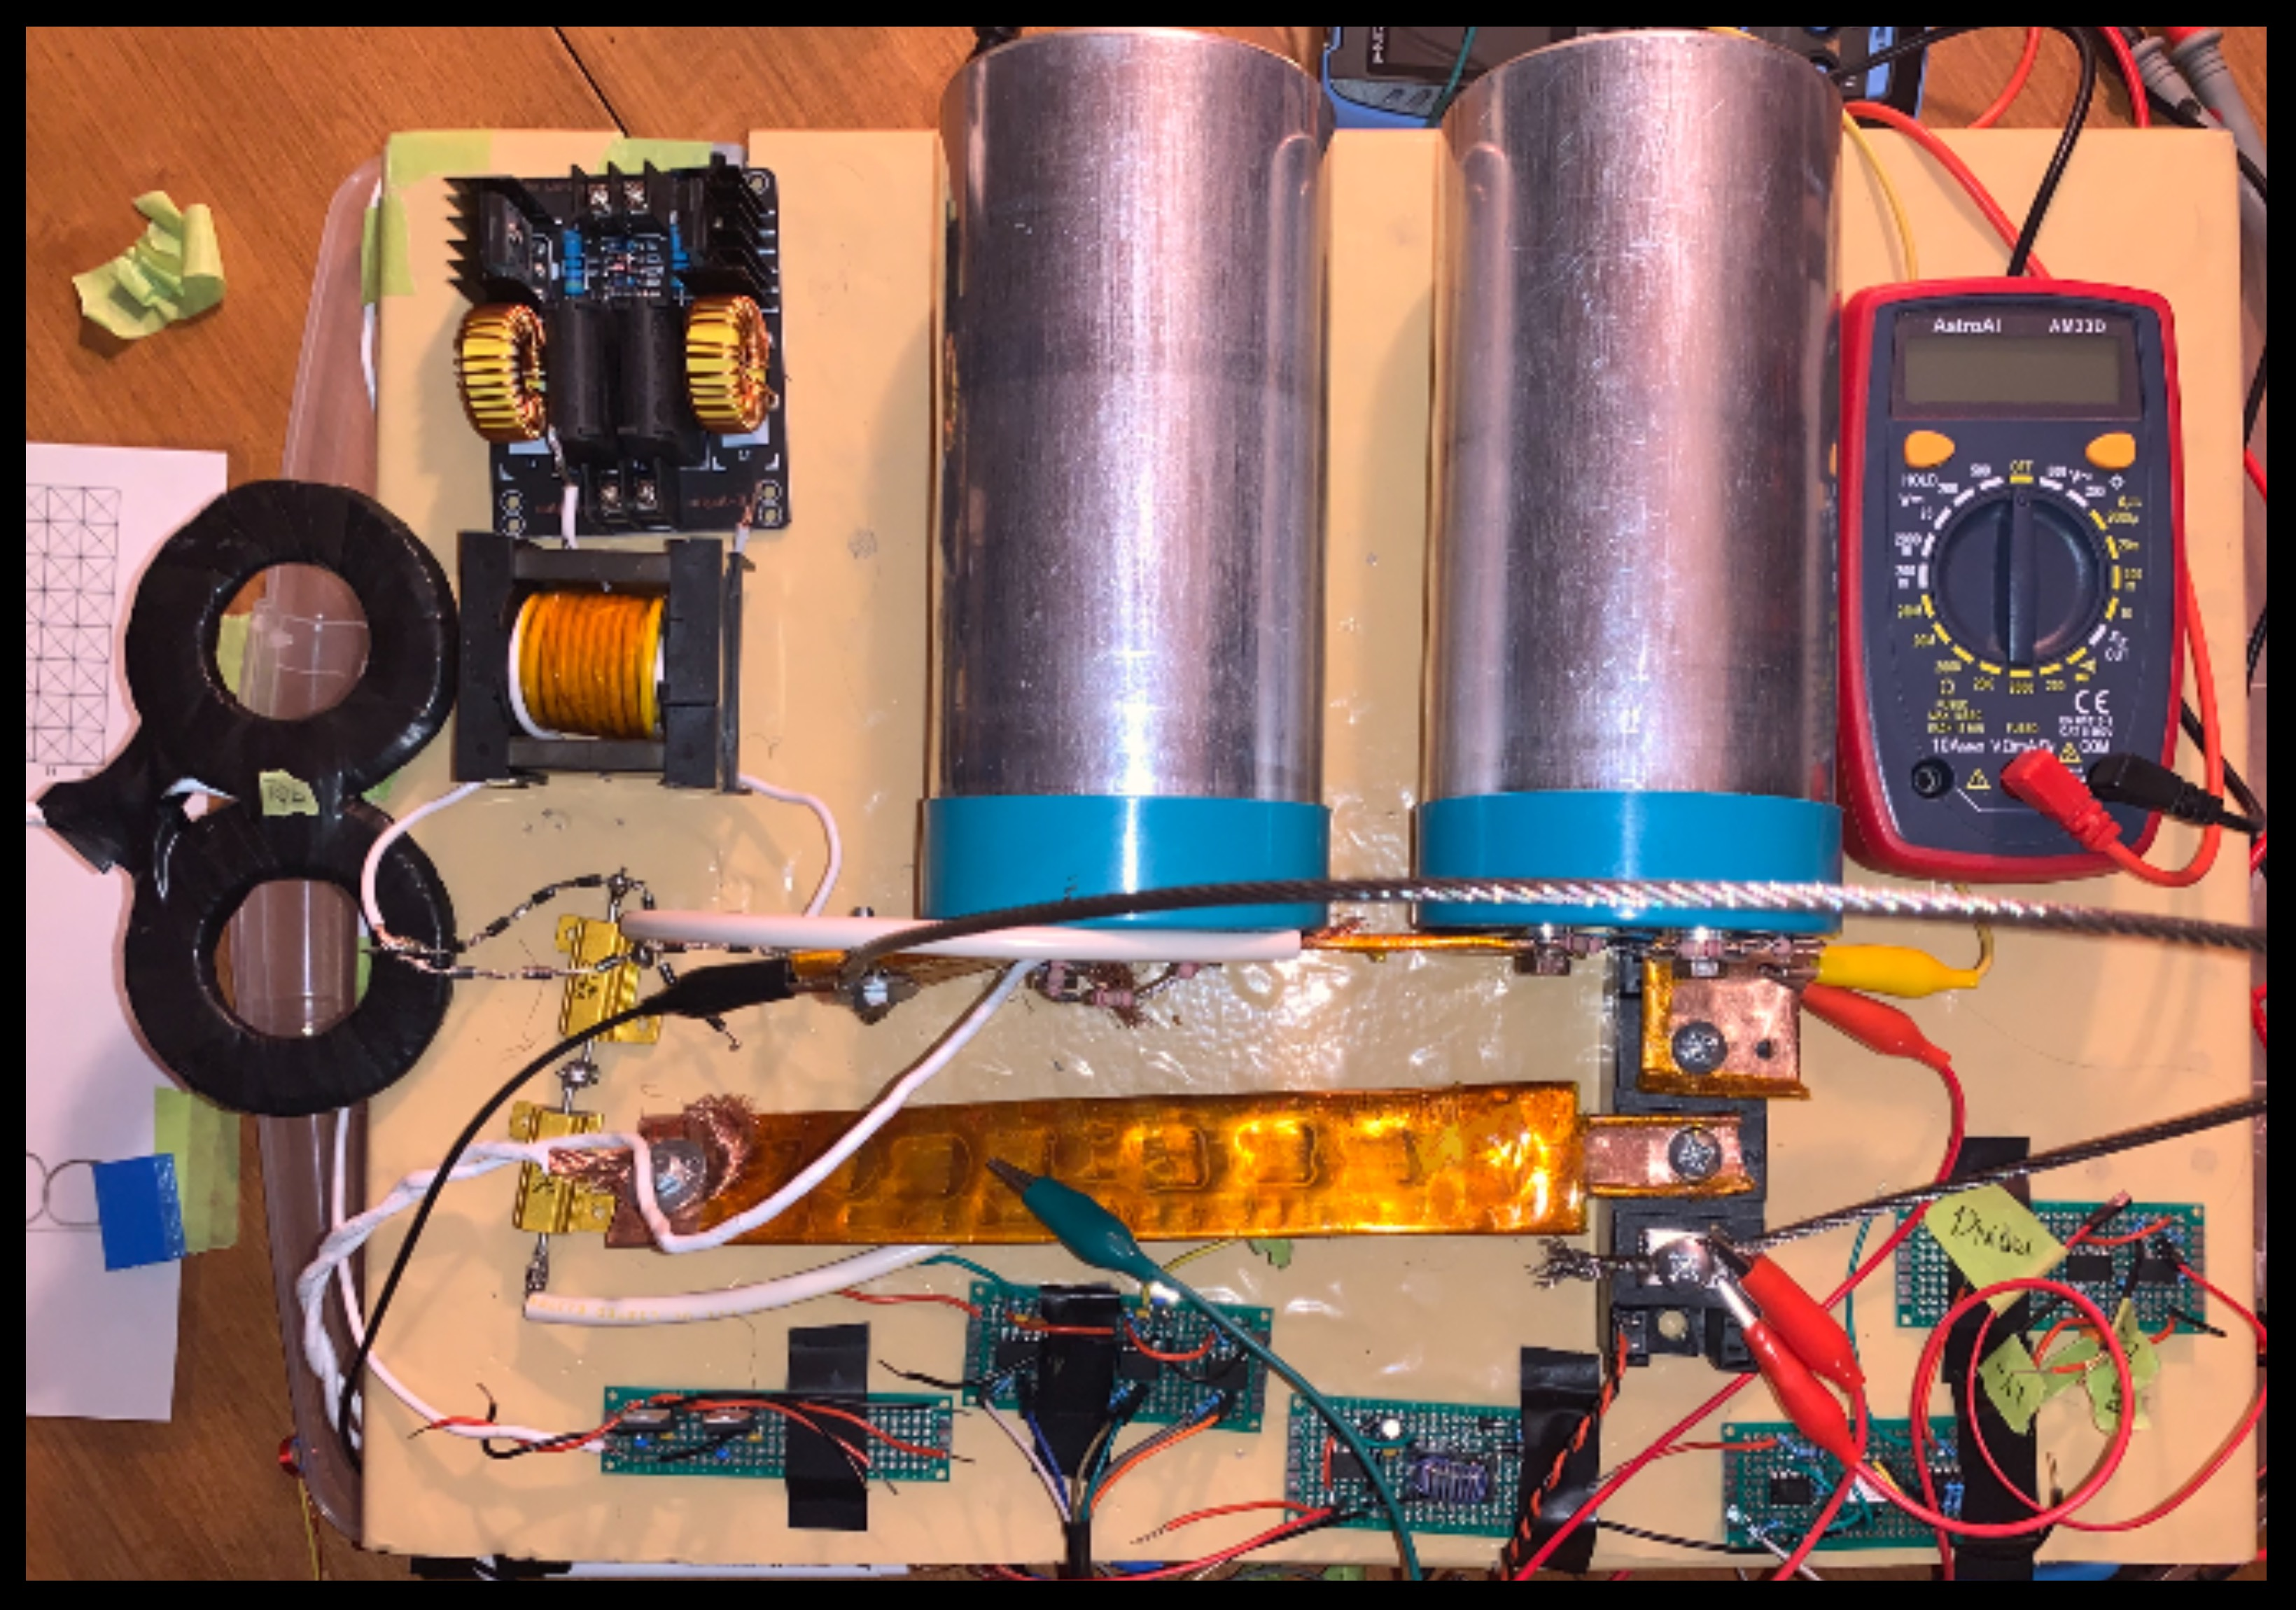
\includegraphics[width=\linewidth,height=23mm,keepaspectratio]{assets/history/mcgill-tms-prototype.jpg}
      \par{\tiny Prototype --- top view\par}\smallskip
      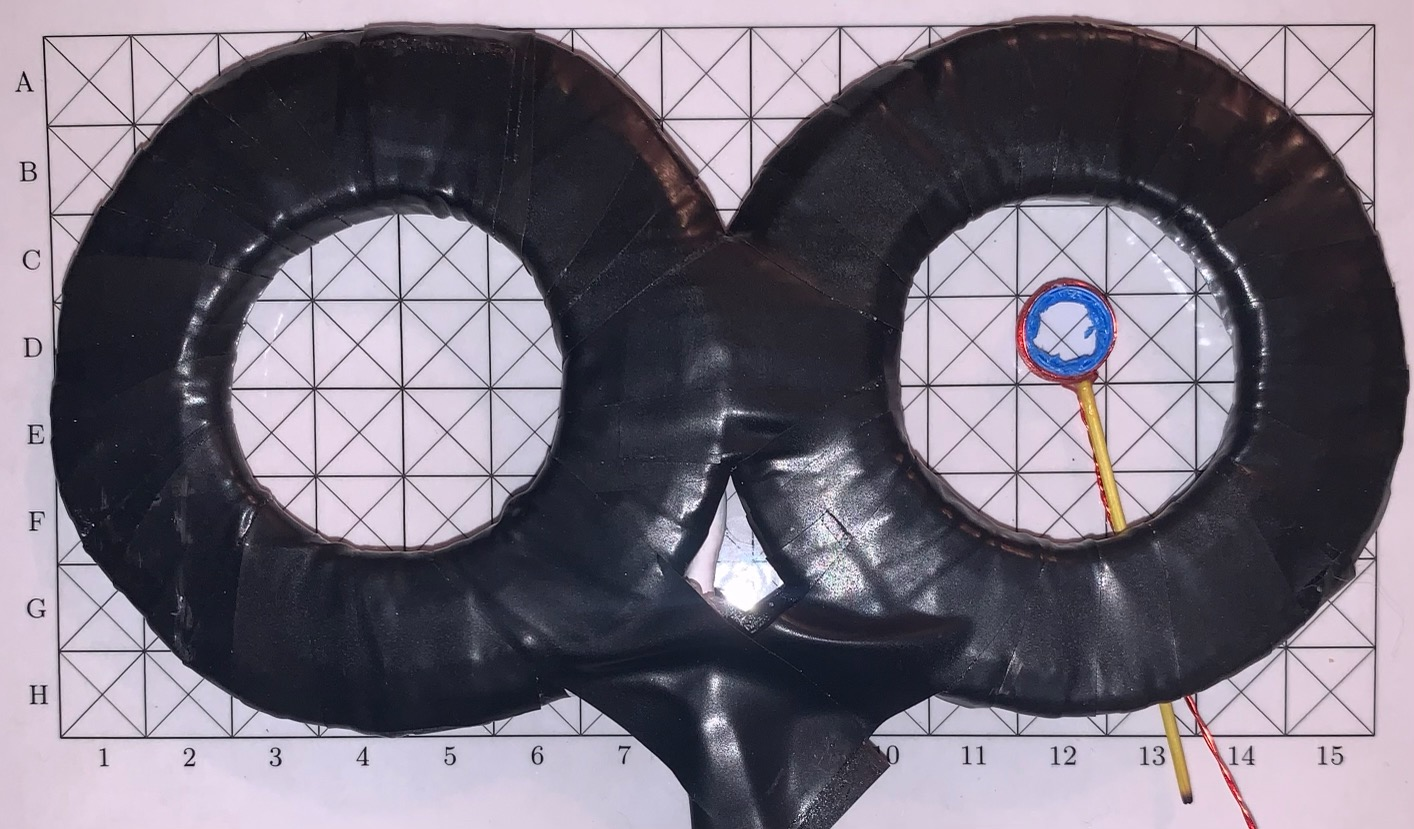
\includegraphics[width=\linewidth,height=21mm,keepaspectratio]{assets/history/mcgill-tms-coil.jpg}
      \par{\tiny Coil and field-measurement setup\par}
  \end{columns}
  {\tiny\color{NTXMuted}Sources: \href{https://www.linkedin.com/posts/maxence-lapatrie_brain-stimulation-research-can-be-expensive-activity-7498376586744709120-7w6N}{team announcement}; \href{https://doi.org/10.64898/2026.08.25.747050}{bioRxiv, August 2026}; photos: \href{https://www.mcgill.ca/ose/files/ose/2-35_-_maxence.pdf}{McGill project poster}\par}
  \note{[67:15--68:45] McGill NeuroTech announced the hardware team's new preprint. Credit Maxence Lapatrie, Yuzuha Isetani, Jathav Puvirajan, Antonella Catanzaro, Siqi Lyu, Han C. Nguyen, William Mathieu, and Milica Popovic. The preprint reports about USD700 in parts, excluding assumed bench equipment. Characterization combines measured magnetic fields with computational cortical-field estimates on an example anatomy; this is not evidence of demonstrated human stimulation or clinical efficacy. The announcement explicitly says the device is not approved for human stimulation or clinical use. High-energy electrical hardware requires qualified supervision and appropriate safety controls. Photos are extracted from the McGill-hosted project poster, not asserted to show the final preprint revision. Its earlier cost table differs from the new preprint; use the new preprint's rounded cost in the talk. The lesson is the scope of student engineering and characterization, not a DIY treatment recommendation.}
\end{frame}

\begin{frame}{More ambitious student projects: quantum sensors}
  \begin{columns}[c,onlytextwidth]
    \column{.51\textwidth}
      \small
  \NTXPoint{A starting point already exists}{Uncut Gem: an open-source diamond magnetometer from Quantum Village.}
  \NTXPoint{A student challenge}{Build the instrument, characterize its noise, and publish reproducible measurements.}
  \NTXPoint{A longer-term neurotech question}{What would it take to move from a magnetic-field demonstration to useful biosignal sensing?}
    \column{.45\textwidth}
      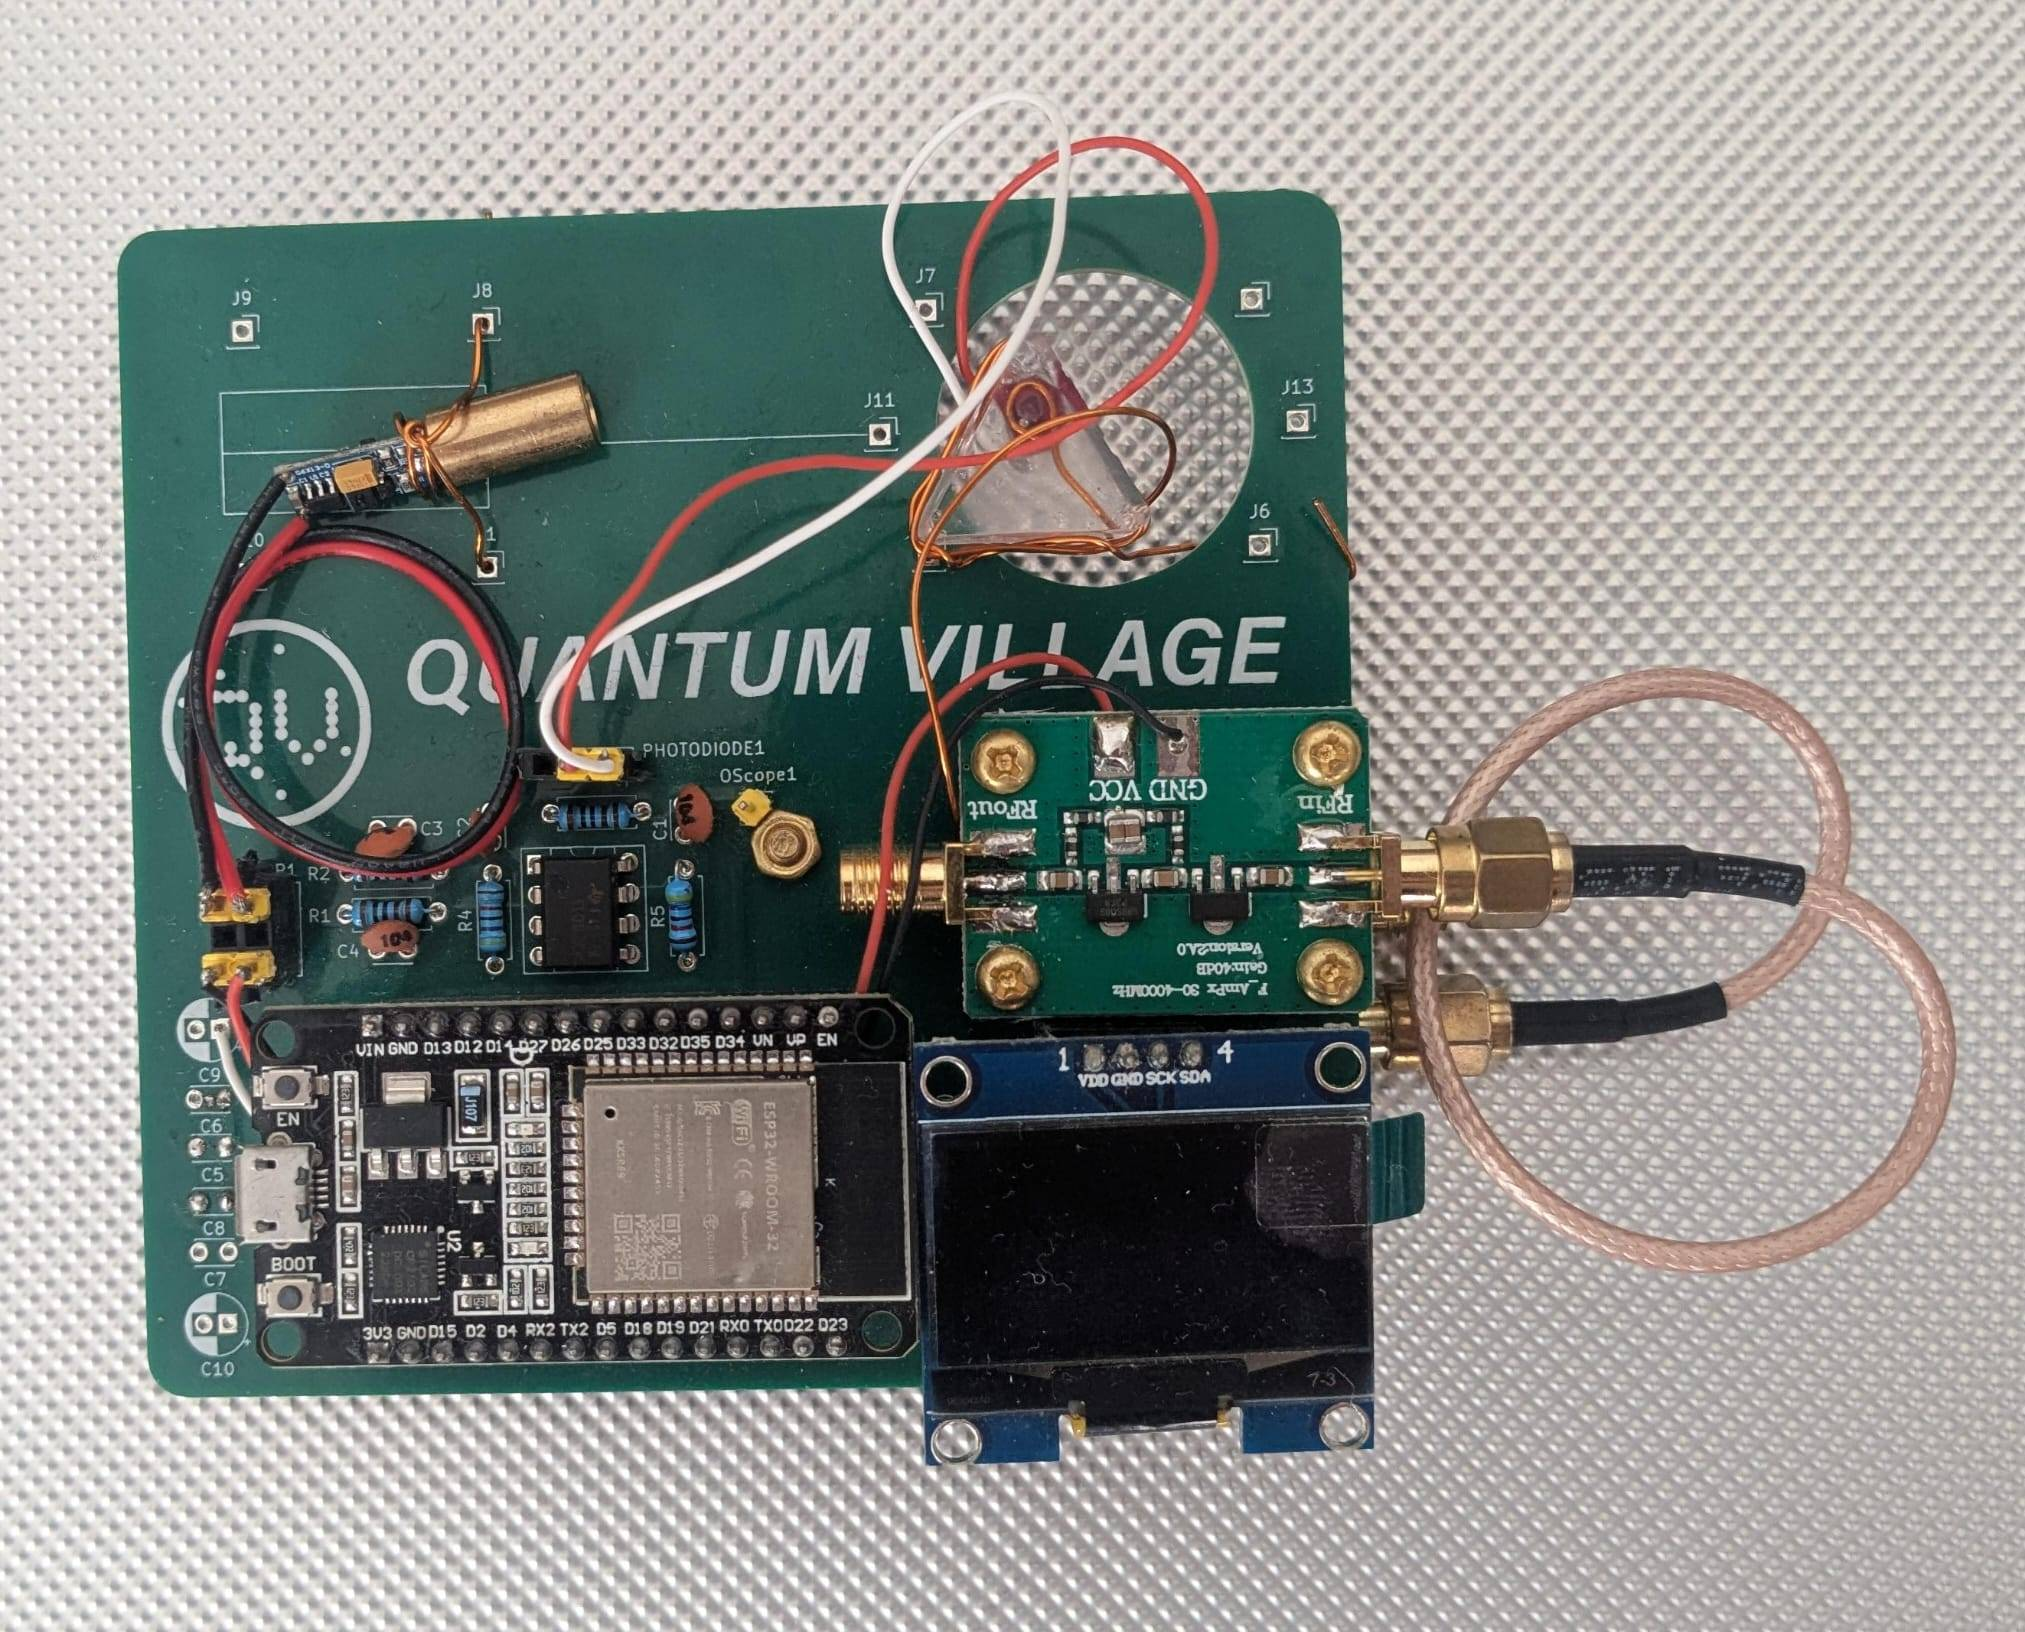
\includegraphics[width=\linewidth,height=45mm,keepaspectratio]{assets/history/uncut-gem-prototype.jpeg}\par\smallskip
      {\scriptsize Uncut Gem prototype\newline Photo: \href{https://quantumvillage.org/uncut-gem.html}{Quantum Village}\par}
  \end{columns}
  \NTXSource{https://arxiv.org/abs/2509.18329}{Carney and Kumaran: Uncut Gem; proposed student challenge, not an announced NTX program}
  \note{[68:45--70:15] Nitrogen-vacancy centers in diamond provide a concrete route into quantum sensing. The project publishes hardware and firmware. This is a learning platform, not a demonstrated brain scanner. Propose characterization and reproducibility as meaningful student contributions. Brain-field sensitivity is a separate research challenge; do not imply that assembling this kit produces an MEG instrument. Work requires appropriate equipment training and supervision.}
\end{frame}

\begin{frame}{Build an MRI: Johns Hopkins, September 16--18}
  \begin{columns}[c,onlytextwidth]
    \column{.50\textwidth}
      \small
  \NTXPoint{Coming up: DELTA DIY-MRI 2026}{Three days at Johns Hopkins University in Baltimore: learn, design, build, and scan.}
  \NTXPoint{A mentored, hands-on team project}{Build low-field MRI components and image a phantom: magnets, RF and gradient coils, acquisition, and reconstruction.}
  \NTXPoint{Free attendance; currently sold out}{Join the waitlist, or explore the public build resources and community.}
    \column{.46\textwidth}
      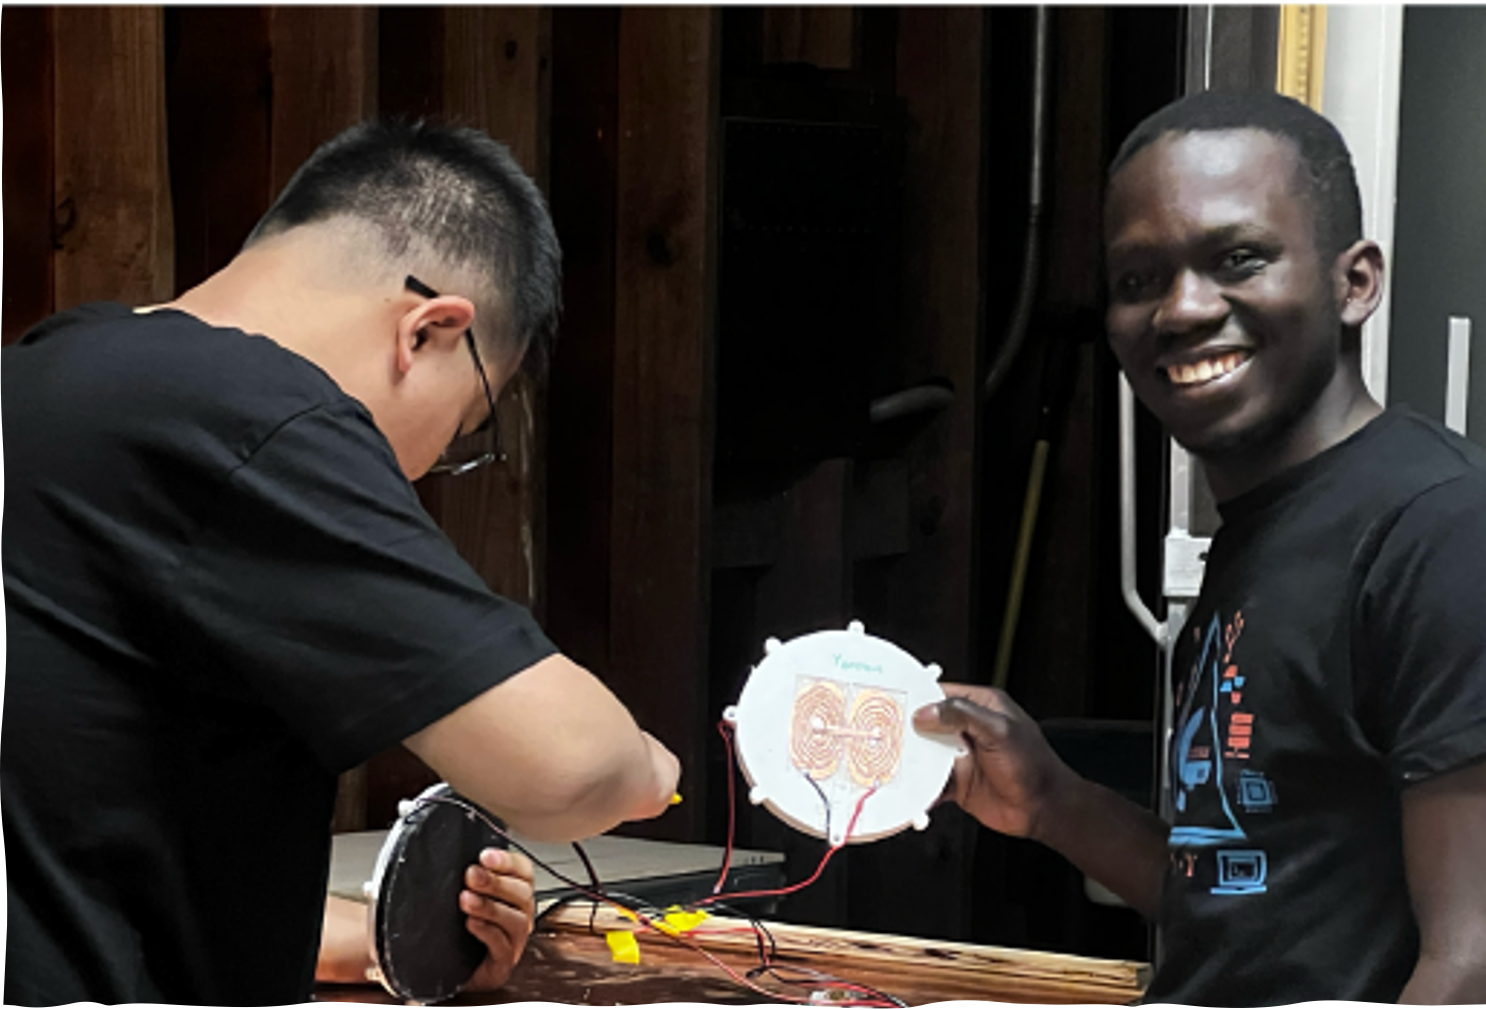
\includegraphics[width=\linewidth,height=42mm,keepaspectratio]{assets/history/jhu-diy-mri-build.png}\par\smallskip
      {\scriptsize Earlier workshop: hands-on building\newline Photo: DELTA DIY-MRI organizers\par}
  \end{columns}
  \NTXSource{https://delta-diy-mri.github.io/}{delta-diy-mri.github.io --- September 16--18, 2026; waitlist and resources}
  \note{[70:15--71:45] Announce the upcoming DELTA DIY-MRI workshop at Johns Hopkins University, Baltimore, September 16--18, 2026: nine days after this September 7 presentation. The official page checked September 6 says attendance is free but sold out, with a waitlist; do not promise a place. Its public wiki, repository and GitHub Discussions offer another route to participate. The picture is an earlier workshop photograph supplied on the organizer's site, not a photograph of the upcoming event. The previous event was May 5--7, 2025, not August 2026. This is an independent workshop, not an NTX-organized event. Mentored work covers magnet, RF, gradients, acquisition and reconstruction, ending in phantom imaging, not human scanning. The broader precedent remains MRI4ALL's four-day 2023 build. A student adaptation requires prepared components, expert mentors and magnet, RF, electrical and mechanical safety oversight.}
\end{frame}

\begin{frame}{LIBRE Hub: sharing an MRI build in Paraguay}
  \begin{columns}[T,onlytextwidth]
    \column{.62\textwidth}
      \NTXPoint{Open bioimaging across communities}{LIBRE Hub connects scientists, engineers, and makers in Latin America and beyond.}
      \NTXPoint{OSI2ONE in Asunci\'on}{Joshua Harper's team at Universidad Paraguayo Alemana described building an open low-field MRI.}
      \NTXPoint{Share what it takes to build}{Construction experience and practical considerations, presented in a June 2024 seminar.}
    \column{.32\textwidth}
      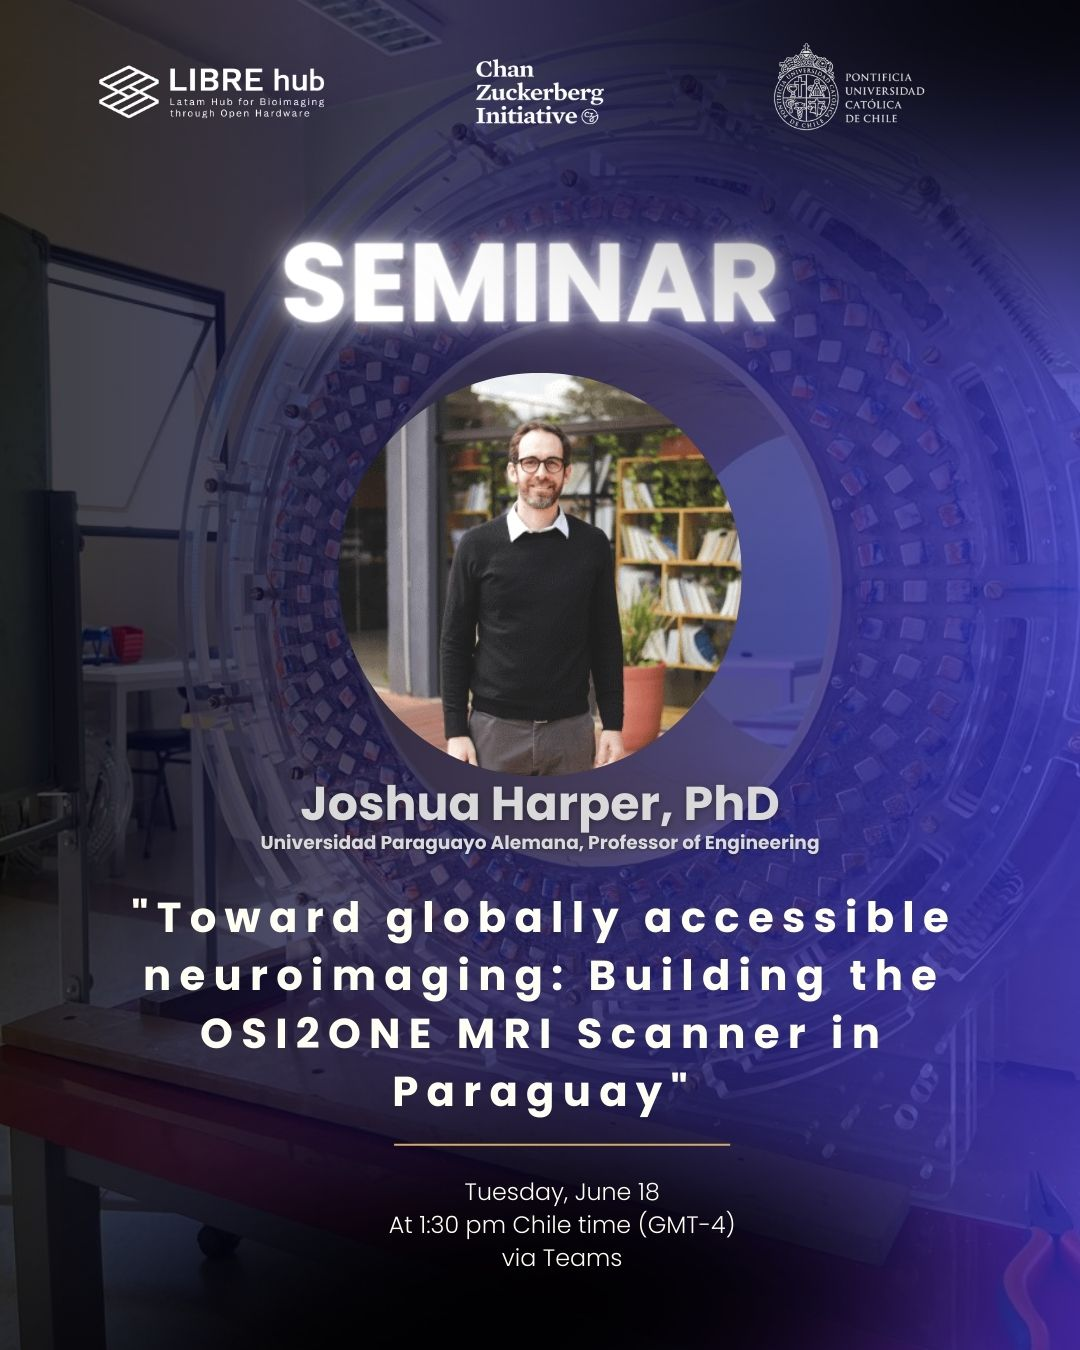
\includegraphics[width=\linewidth,height=49mm,keepaspectratio]{assets/history/librehub-paraguay-mri-2024.jpg}
      \par\smallskip{\scriptsize Original LIBRE Hub announcement\par}
  \end{columns}
  {\tiny\color{NTXMuted}Sources: \href{https://librehub.github.io/}{LIBRE Hub}; \href{https://librehub.github.io/2024/06/05/joshua-harper.html}{Joshua Harper seminar, 18 June 2024}; \href{https://youtu.be/NiABwvTVwp8}{recording}\par}
  \note{[71:45--73:15] LIBRE Hub is the dissemination and training community, not the builder or owner of this MRI project. The June 18, 2024 seminar describes a build underway at Universidad Paraguayo Alemana in Asuncion, Paraguay, using the Open Source Imaging Initiative's OSI2ONE design, intended for a neuroimaging project at a clinic in Bolivia. This source does not establish completed installation or clinical use in Bolivia. The image is the seminar flyer, not a documentary photograph of a completed Paraguayan scanner. Keep distinct from MRI4ALL's four-day build; no weekend completion claim is made for Paraguay. The lesson is locally developed expertise supported by shared designs and practical teaching.}
\end{frame}

\begin{frame}{CONNExIN: building expertise, looking toward Lagos}
  \begin{columns}[c,onlytextwidth]
    \column{.67\textwidth}
      \small
  \NTXPoint{Udunna Anazodo and the CONNExIN team}{Hybrid, hands-on neuroimaging training: developing local experts who can train others.}
  \NTXPoint{A shared contribution at ISMRM 2026}{Draper et al., abstract 563-01-002.\newline Morgan Hough, NeuroTechX --- co-author.}
  {\scriptsize\itshape Training 105 African clinicians and students in open neuroimaging analysis: CAMERA's dementia research program\par}
  \medskip
  \NTXPoint{Our hope for Lagos}{To become the first NeuroTechX city chapter in sub-Saharan Africa --- an ambition we hope to realize.}
    \column{.28\textwidth}
      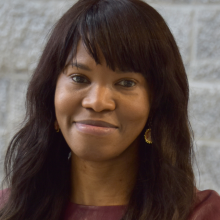
\includegraphics[width=\linewidth,height=35mm,keepaspectratio]{assets/people/udunna-anazodo.png}\par\smallskip
      {\small Udunna Anazodo\par}
      {\tiny Portrait: \href{https://mcmedhacks.com/team/dr-udunna-anazodo/}{McMedHacks}\par}
  \end{columns}
  {\tiny\color{NTXMuted}Sources: \href{https://event.fourwaves.com/connexin/pages/41f08c9e-6502-46b4-bf53-ec5a6cf095b7}{CONNExIN program}; \href{https://echo.ismrm.org/abstracts/view/a98f4909-2b73-49d0-849b-14f932d68bca}{ISMRM 2026 abstract}; Lagos aspiration: Morgan Hough\par}
  \note{[73:15--74:45] The official program spelling is CONNExIN. Credit Udunna Anazodo and the whole team. Its organizers describe a free hybrid train-the-trainer initiative connecting the MiND Lab at the Montreal Neurological Institute with McGill's aging research centre, the Medical Artificial Intelligence Lab in Nigeria, and CAMERA. Team-based learning builds local neuroimaging expertise. The 2025 program lists the MAI Lab in Lagos as its hybrid location. The accepted ISMRM 2026 digital-poster abstract is Training 105 African clinicians and students in open neuroimaging analysis: CAMERA's dementia research program, presented by Ethan Draper in Cape Town on May 13. Morgan is listed as a co-author with NeuroTechX affiliation. The title's 105 is not independently verified as a completion or certification count: the full abstract and results are access-restricted and were not read. Our hope is for Lagos to become the first NTX city chapter in sub-Saharan Africa. This is Morgan's aspiration, not a claim that a chapter has launched or an independently audited first-ever ranking. The public NTX directory mentions Lagos without proving launch status. Do not conflate this with the existing ISMRM African Chapter or imply that NTX owns CONNExIN.}
\end{frame}


\begin{frame}{From making almost anything to growing almost anything}
  \begin{columns}[c,onlytextwidth]
    \column{.66\textwidth}
      \small
      \setlength{\medskipamount}{3pt}
      \NTXPoint{1998 --- How to Make (Almost) Anything}{Neil Gershenfeld's MIT course: learn fabrication by building.}
      \NTXPoint{2001 onward --- CBA / Fab Labs}{Center for Bits and Atoms: information meets fabrication. Fab Labs share tools; Fab Academy connects local learning.}
      \NTXPoint{2015 --- How to Grow (Almost) Anything}{Distributed synthetic biology education through Fab Labs and community biology labs.}
      \NTXPoint{2019 / 2021 --- Campus to global classrooms}{MIT/Harvard offering in 2019; remote experiments, robotics, and mentoring in the 2021 redesign.}
    \column{.30\textwidth}
      \centering
      
\includegraphics[width=\linewidth,height=23mm,keepaspectratio]{assets/history/cba-official-logo.jpg}
      \par\bigskip
      
\includegraphics[width=\linewidth,height=19mm,keepaspectratio]{assets/history/htgaa-logo.pdf}
      \par\smallskip{\scriptsize How to Grow (Almost) Anything\par}
  \end{columns}
  {\tiny\color{NTXMuted}Sources: \href{https://betterworld.mit.edu/spectrum/issues/spring-2018/how-to-make-almost-anything-better/}{MIT: HTMAA}; \href{https://cba.mit.edu/about/}{CBA}; \href{https://fabfoundation.org/getting-started/}{Fab Foundation}; \href{https://www.media.mit.edu/articles/a-global-lab-for-teaching-and-practicing-synthetic-biology/}{MIT: HTGAA history}\par}
  \note{[74:45--76:15] MIT's official course name is How to Make (Almost) Anything, abbreviated HTMAA, rather than HTBAA. Gershenfeld began it in 1998. CBA launched with NSF support in 2001, studying the relationship between information and physical things. Fab Labs extend access to fabrication tools; Fab Academy distributes instruction across local labs. These are related, not interchangeable institutions. HTGAA began globally in 2015, drawing on the Fab Lab and community biology networks. David Kong and George Church offered it to MIT and Harvard graduate students in 2019; Joseph Jacobson is also credited as an instructor. In 2021, remote robotic experiments and mentoring supported distributed participation. The connection to Biopunk Lab here is the community-learning model, not a claim of formal MIT, Fab Lab, or HTGAA affiliation.}
\end{frame}

\begin{frame}{From using chips to learning how to make them}
  \begin{columns}[c,onlytextwidth]
    \column{.47\textwidth}
      \small
      \NTXPoint{Hacker Fab: open fabrication}{Student-built tools, shared processes, and device characterization.}
      \NTXPoint{Demonstrated at CMU}{Working transistors, including self-aligned NMOS devices.}
      \NTXPoint{Our next ambition}{Explore CMOS access and custom sensor electronics through fabrication communities.}
    \column{.49\textwidth}
      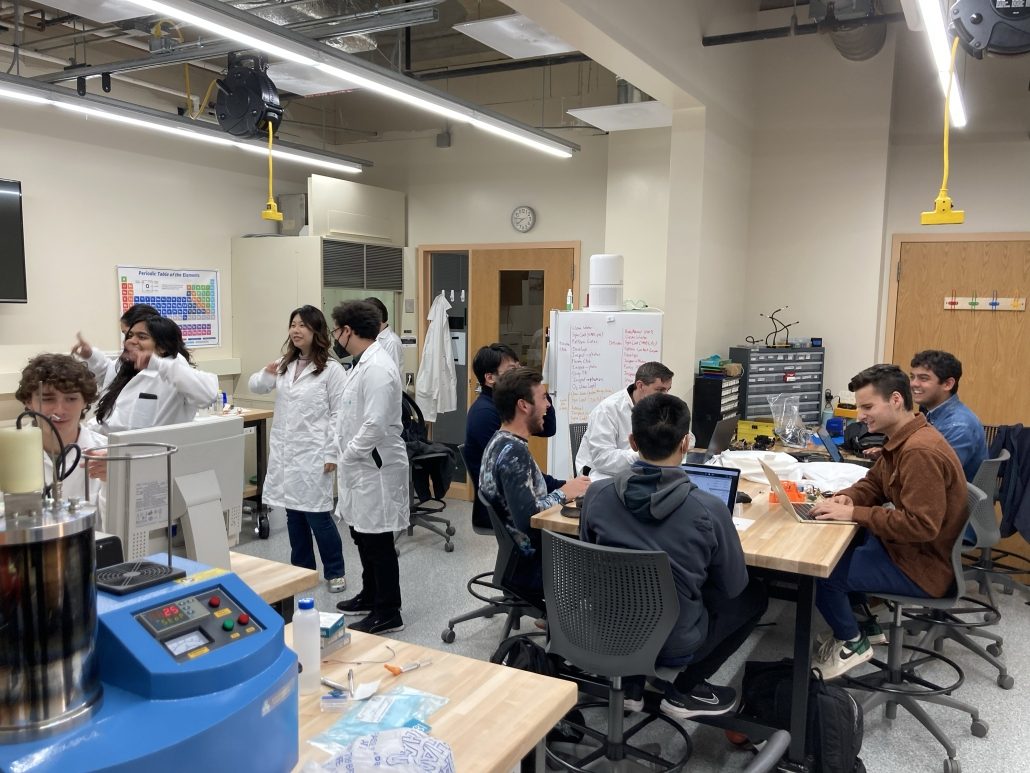
\includegraphics[width=\linewidth,height=45mm,keepaspectratio]{assets/history/hackerfab-cmu-lab.jpg}
      \par\smallskip{\scriptsize Inside Hacker Fab at Carnegie Mellon\par}
  \end{columns}
  \NTXSource{https://hackerfab.ece.cmu.edu/}{Hacker Fab at Carnegie Mellon University; CMOS access is a proposed direction}
  \note{[76:15--77:45] Hacker Fab started at CMU in 2023. Its documented NMOS demonstration should not be relabeled as a complete CMOS process or a commercial foundry service. The relevant lesson is access to tools and process knowledge. For neurotech students, projects could span test structures, characterization, and sensor-interface designs as facilities allow. No partnership or fabrication access is promised. Semiconductor processing requires facility-specific chemical, vacuum, thermal, and electrical safety training.}
\end{frame}

\begin{frame}{Biopunk Lab: a home for synthetic neurobiology}
  \begin{columns}[c,onlytextwidth]
    \column{.49\textwidth}
      \small
      \NTXPoint{Back in San Francisco}{Founding Member of Biopunk Lab, working on synthetic neurobiology.}
      \NTXPoint{A place for hands-on work}{Cell culture facility for Neurotech@Berkeley's wetware group.}
      \NTXPoint{Community enables experiments}{Supporting replication work inspired by Mind in Vitro and DishBrain research.}
    \column{.47\textwidth}
      \centering
      
\includegraphics[height=17mm]{assets/history/biopunk-logo.png}
      \par\medskip
      \begin{minipage}[c]{.40\linewidth}
        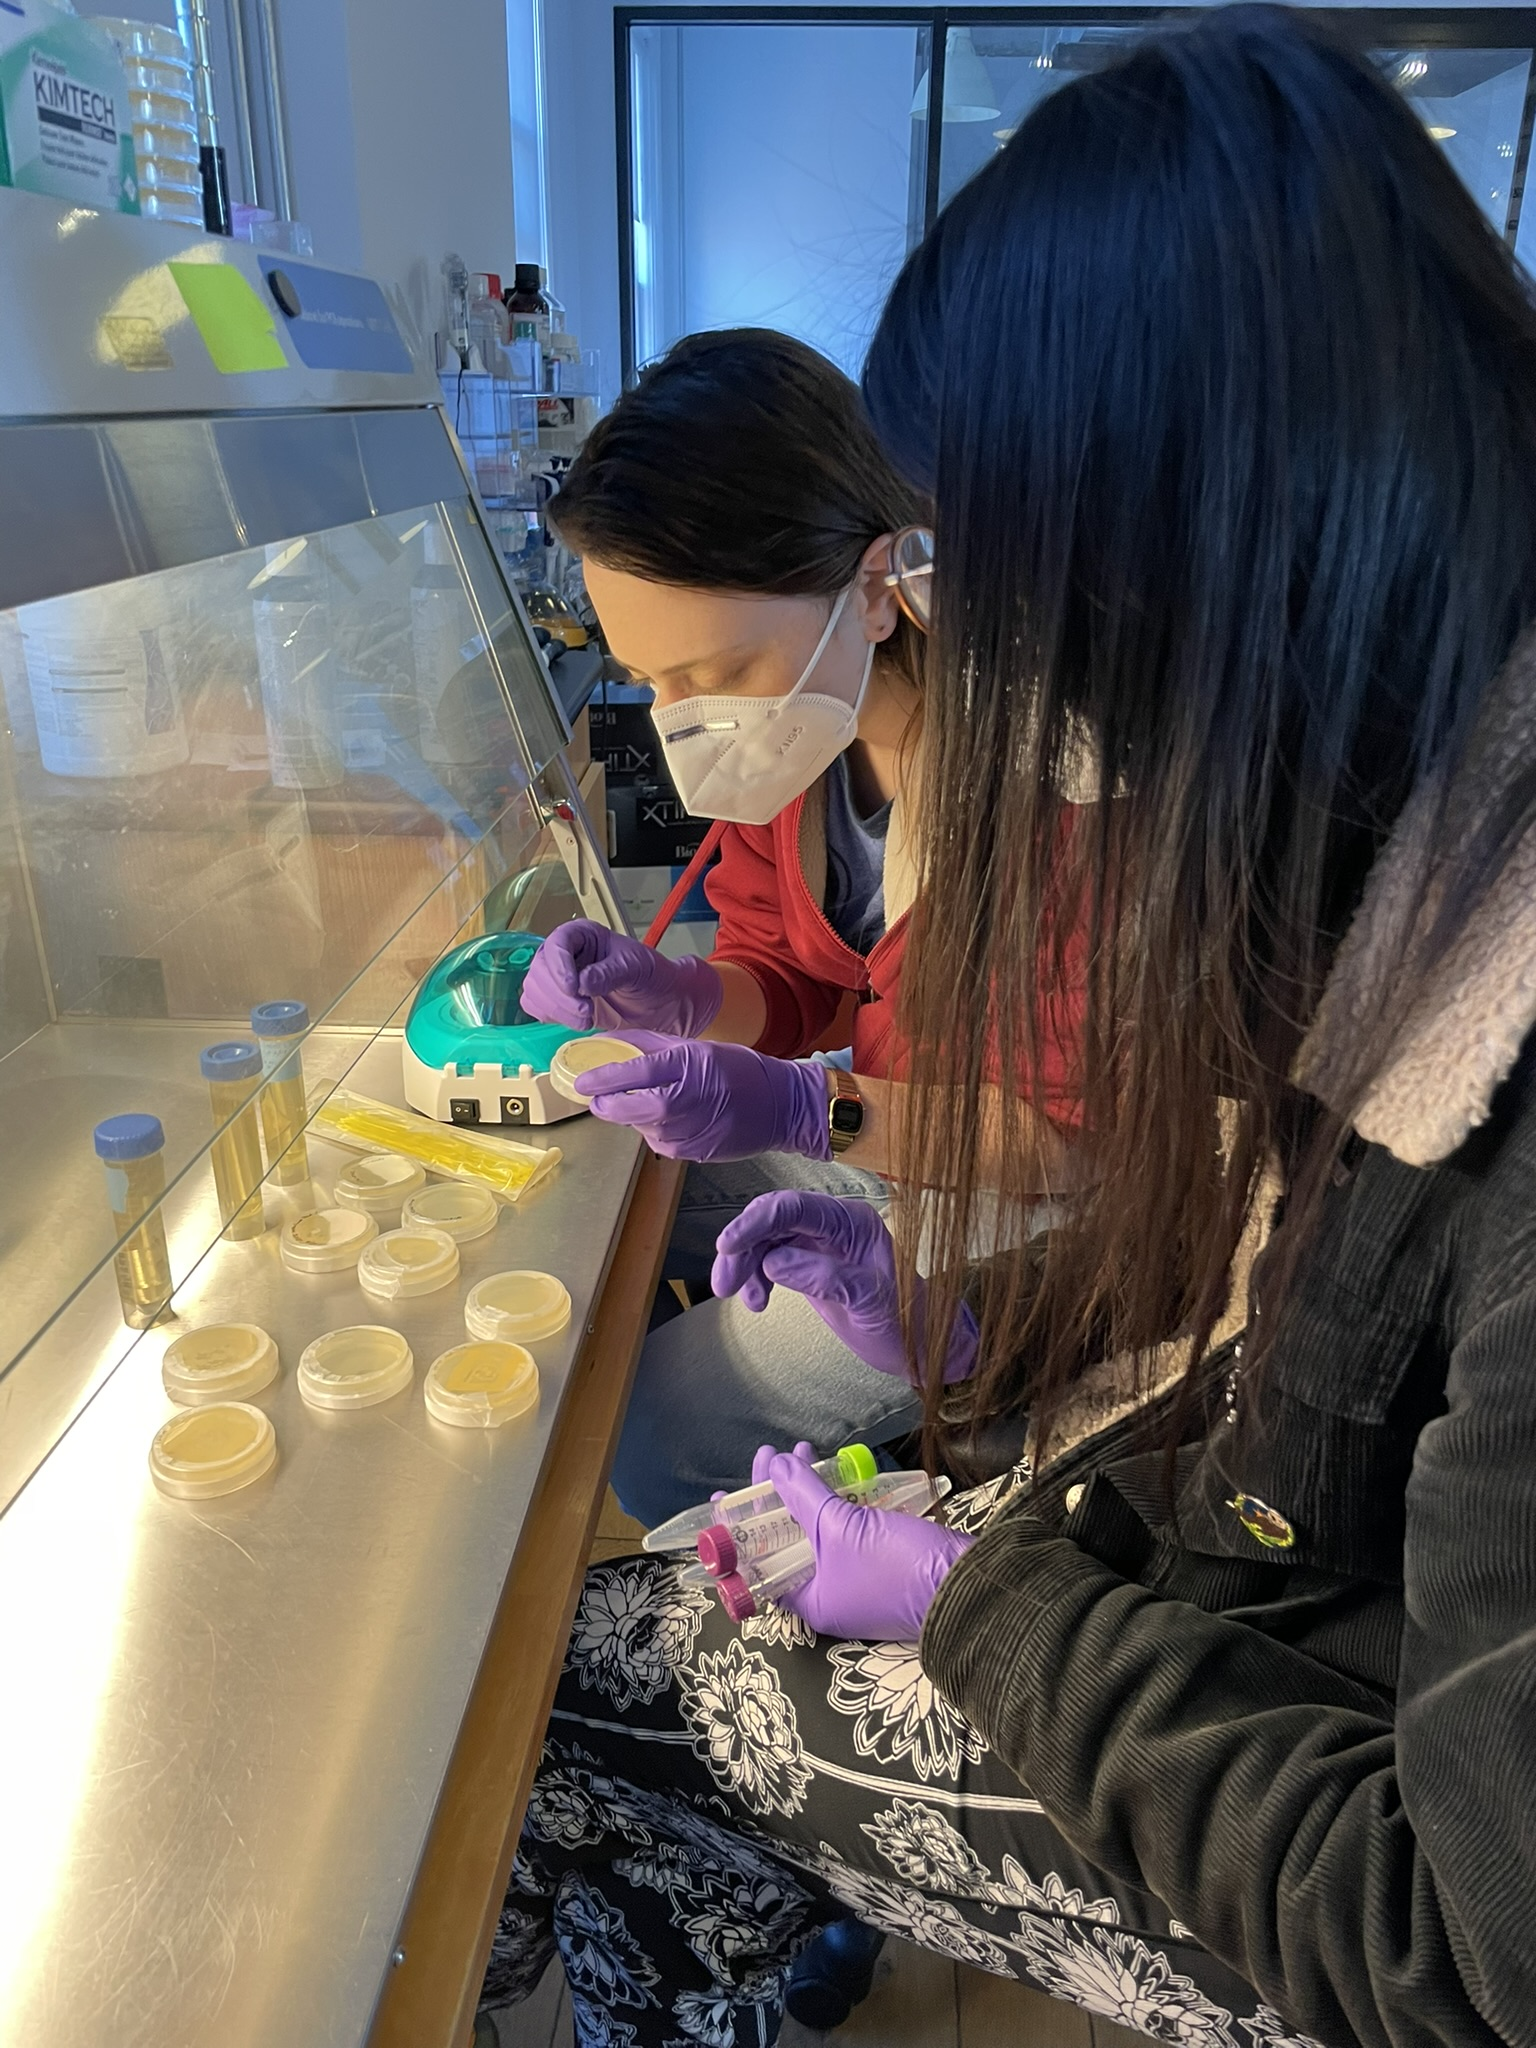
\includegraphics[width=\linewidth,height=31mm,keepaspectratio]{assets/history/biopunk-biosafety.jpeg}
      \end{minipage}\hfill
      \begin{minipage}[c]{.57\linewidth}
        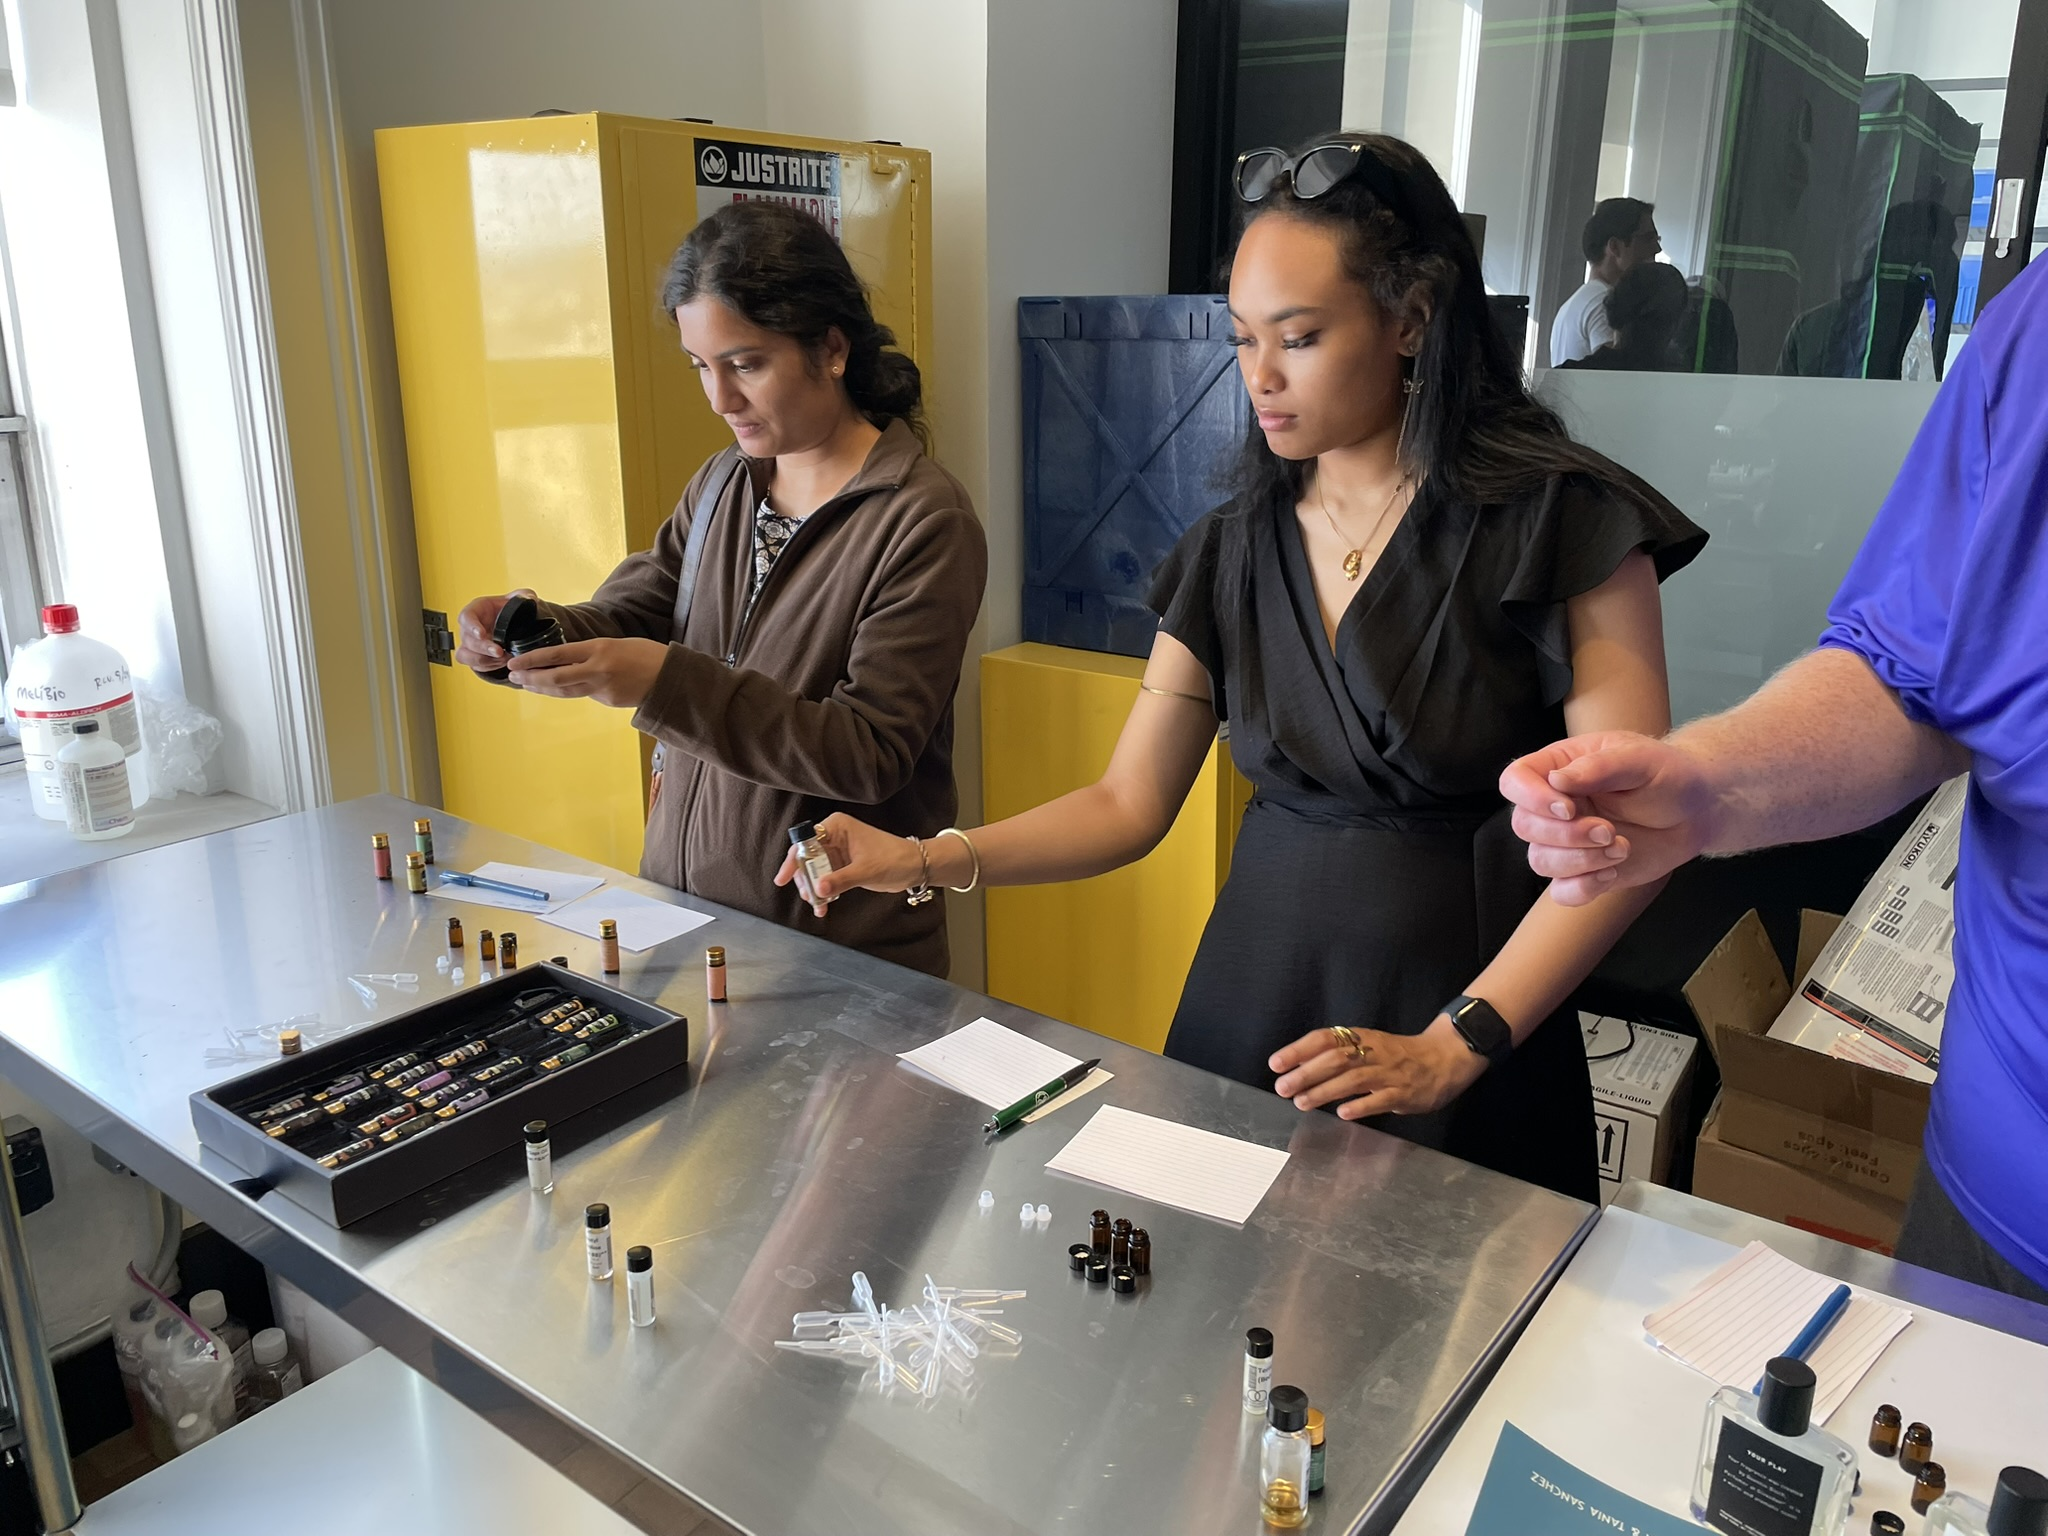
\includegraphics[width=\linewidth,height=31mm,keepaspectratio]{assets/history/biopunk-workshop.jpeg}
      \end{minipage}
      \par\smallskip{\scriptsize Lab work and community workshop\par}
  \end{columns}
  {\tiny\color{NTXMuted}Activities: Morgan Hough's firsthand account. Photos and logo: \href{https://biopunklab.com/}{Biopunk Lab}\par}
  \note{[77:45--79:15] Introduce Biopunk Lab through your experience as a founding member working on synthetic neurobiology. You report that Neurotech@Berkeley's wetware group currently uses the lab as its cell culture facility. This is a firsthand account, not an independently verified institutional announcement. The next slide distinguishes the Illinois Mind in Vitro hardware from Cortical Labs' DishBrain experiments and introduces the Open Ephys collaboration. Describe the work as an effort toward replication, not a completed replication or demonstrated learning result. Cell provenance, biosafety, and ethical oversight remain essential.}
\end{frame}

\begin{frame}{The future of neurobiotech: community wetware}
  \centering
  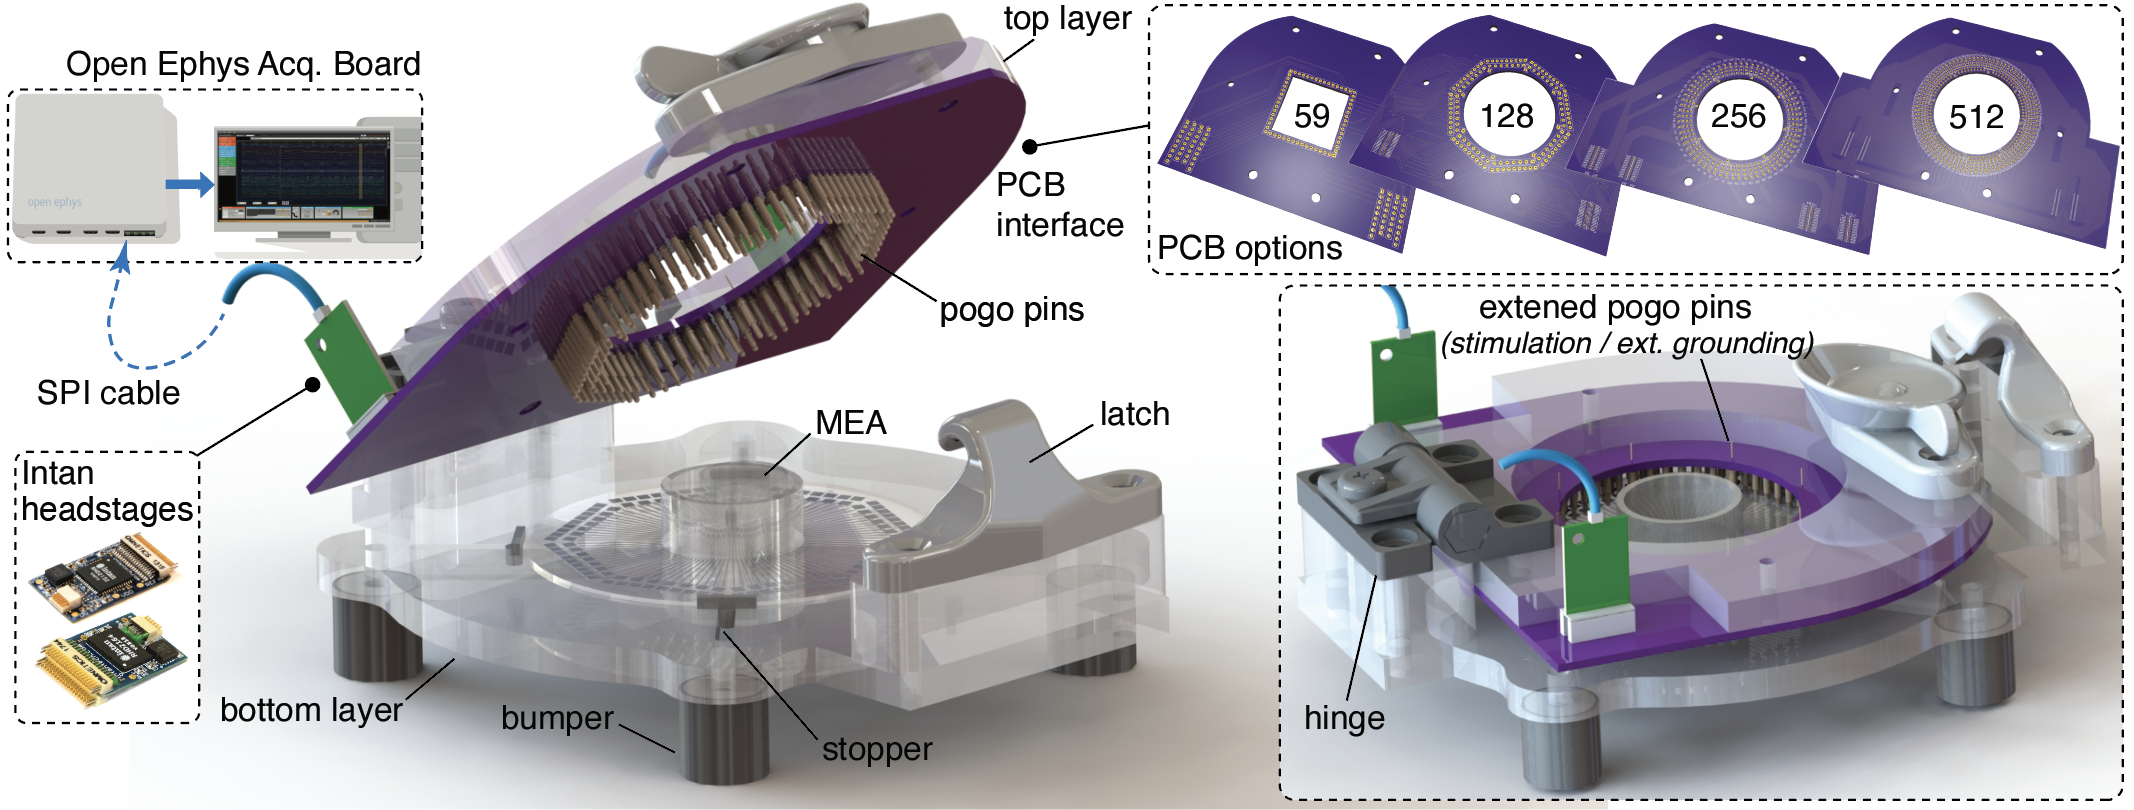
\includegraphics[width=.91\linewidth,height=28mm,keepaspectratio]{assets/history/mind-in-vitro-overview.jpg}
  \par\smallskip
  \raggedright
  {\small
  \textbf{Mind in Vitro as a starting point} --- Open hardware for interfacing with living neurons.\par\smallskip
  \textbf{Working with Open Ephys} --- Developing a low-cost MEA/bioreactor for neuronal stimulation and recording.\par\smallskip
  \textbf{Neurotech@Berkeley wetware at Biopunk Lab} --- Using the cell-culture facility to pursue replication, guided by DishBrain and follow-up studies.\par}
  \medskip
  {\tiny\color{NTXMuted}Image: \href{https://gazzolalab.github.io/MiV-OH/overview/system_overview.html}{MiV-OH / Gazzola Lab}; \href{https://doi.org/10.1002/advs.202306826}{Zhang et al., 2024}; \href{https://doi.org/10.1016/j.neuron.2022.09.001}{DishBrain, 2022}; local work: Morgan Hough\par}
  \note{[79:15--81:15] Morgan reports collaboration with Open Ephys toward a low-cost MEA/bioreactor and Berkeley wetware's current use of Biopunk Lab for cell culture. These are firsthand accounts, not independently verified institutional announcements. The image is the Illinois MiV design, not a completed local device. MiV uses custom MEAs, Intan headstages, Open Ephys acquisition, and modular stimulation/fluidic interfaces. DishBrain (Kagan et al., Neuron 2022) uses a different high-density MEA platform for closed-loop Pong experiments. Follow-ups: Habibollahi et al., Nature Communications 2023, on critical dynamics; Khajehnejad et al., 2024 preprint arXiv:2405.16946, on sample efficiency. Full citations are in assets/history/mind-in-vitro-sources.md. Hardware replication is distinct from reproducing behavioral results; no completed Berkeley replication, learning, or sentience result is claimed. Appropriate cell provenance, biosafety, and ethical oversight remain necessary.}
\end{frame}

\begin{frame}{Marley Xiong and collaborators: projects to Aleph}
  \begin{columns}[c,onlytextwidth]
    \column{.49\textwidth}
      \small
      \NTXPoint{Student community: McGill NeuroTech}{Marley Xiong, Raffi Hotter, and fellow students: Milo, NTX competition 2019.}
      \NTXPoint{Brainhack: testing a difficult idea}{A ten-day acoustoelectric tank proof of concept with collaborators.}
      \NTXPoint{Aleph: continuing the ambition}{Marley, Raffi, and Lev Chizhov: announced cofounders.}
    \column{.47\textwidth}
      \centering
      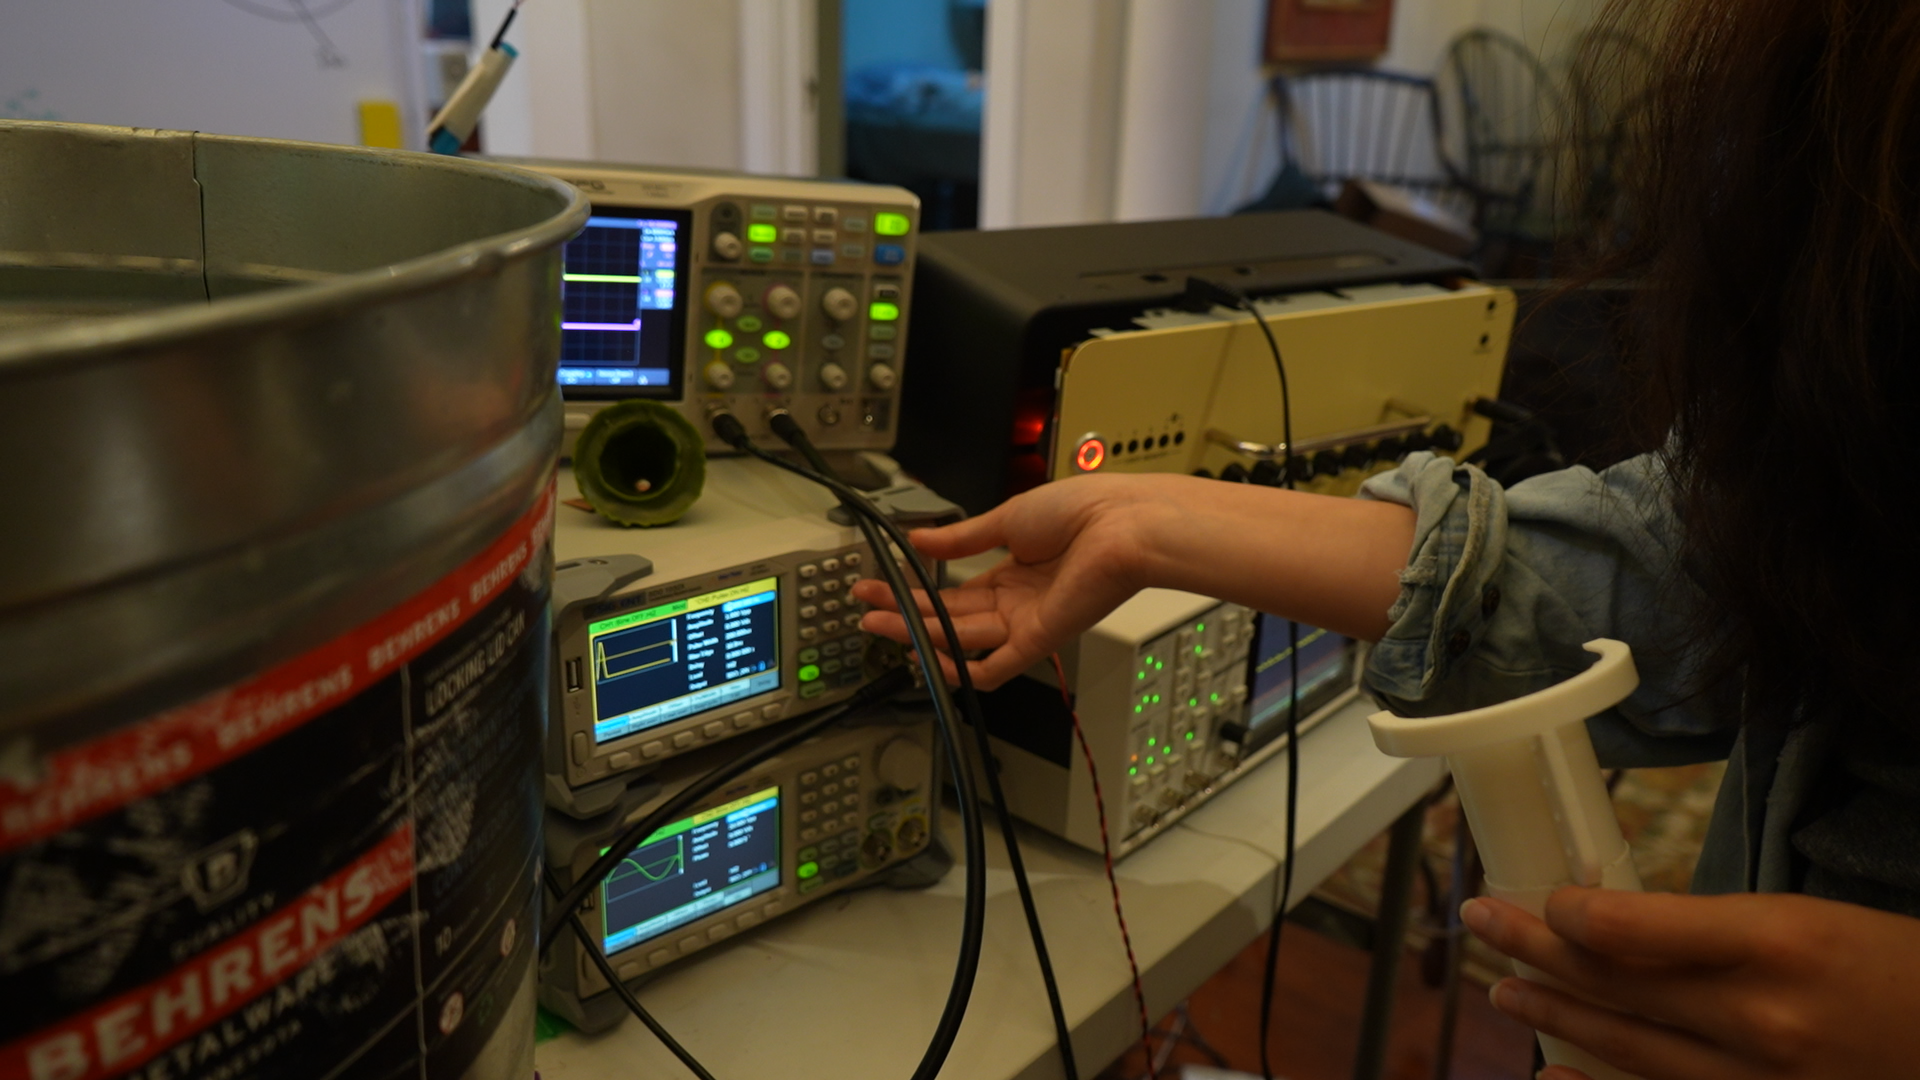
\includegraphics[width=\linewidth,height=24mm,keepaspectratio]{assets/history/brainhack-ae-workbench.png}
      \par\smallskip
      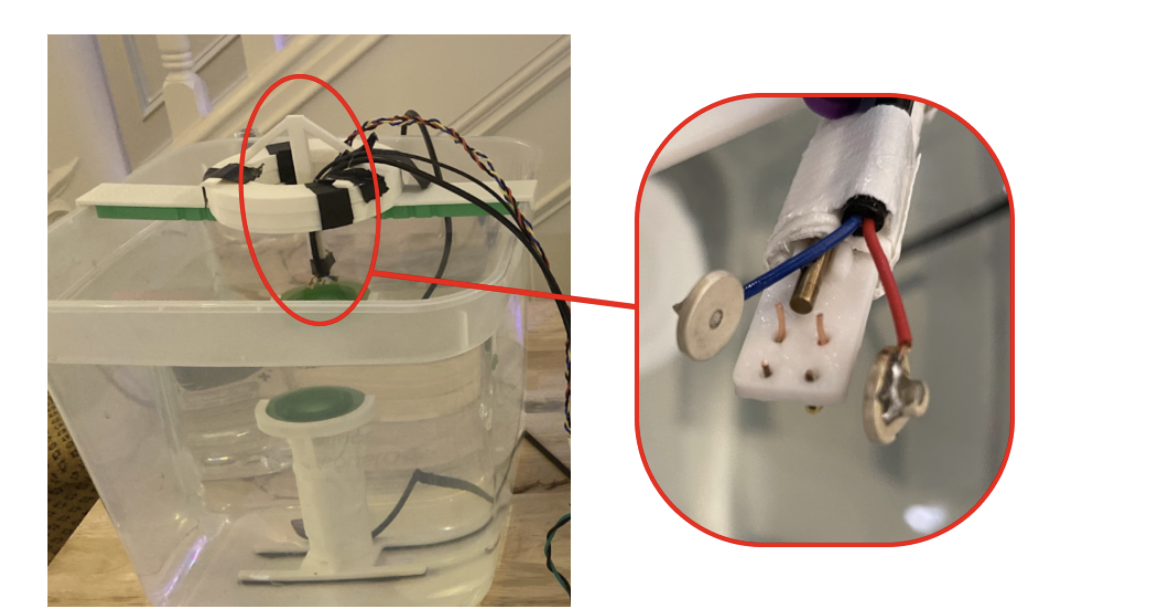
\includegraphics[width=\linewidth,height=23mm,keepaspectratio]{assets/history/brainhack-ae-probe.png}
      \par\smallskip{\scriptsize Brainhack: workbench and tank probe\par}
  \end{columns}
  {\tiny\color{NTXMuted}Sources: \href{https://reporter.mcgill.ca/meet-milo-mcgills-brain-powered-wheelchair/}{McGill Reporter}; \href{https://brainhack.vercel.app/ae}{Brainhack project}; \href{https://www.linkedin.com/posts/marley-xiong_on-thursday-we-shared-the-most-detailed-scan-activity-7476685168531988480-xSam}{Marley's Aleph announcement}\par}
  \note{[81:15--83:15] Credit the teams, not only the later founders. The Brainhack AE page names Ethan Childerhose, Kevin Chung, Andy Kong, Brian Machado, and Marley Xiong. It describes a tank experiment, not a demonstrated human neural interface. Morgan supplies the broader Brainhack-to-Aleph narrative; public sources verify these milestones and overlapping participants, not a formal spinout or a causal claim that NTX created Aleph. Aleph's brain-interface aspirations are not demonstrated telepathy. Invite Morgan's firsthand account of how relationships and shared work continued.}
\end{frame}

\NTXDivider{Education is Changing}

\begin{frame}{Neuromatch: changing who can learn the methods}
  \begin{columns}[c,onlytextwidth]
    \column{.46\textwidth}
      \small
      \NTXPoint{An open curriculum}{Computational neuroscience, deep learning, and NeuroAI beyond a single university.}
      \NTXPoint{Learning with other people}{Coding, teaching-assistant support, and shared projects.}
      \NTXPoint{An opportunity for our chapters}{Study groups that carry shared learning into local projects.}
    \column{.50\textwidth}
      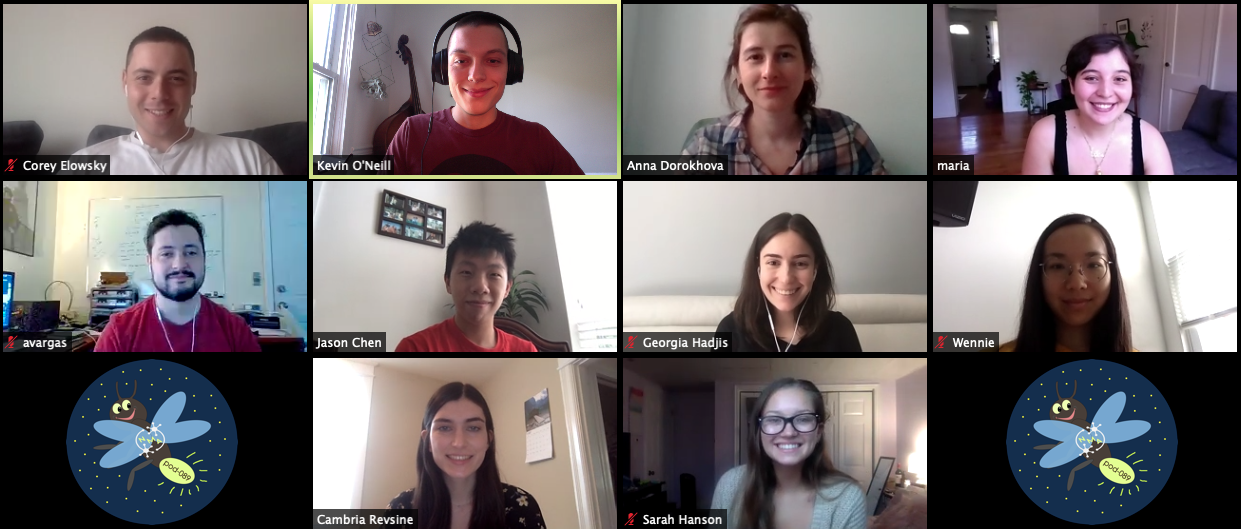
\includegraphics[width=\linewidth,height=44mm,keepaspectratio]{assets/history/neuromatch-pod-2020.png}
      \par\smallskip{\scriptsize Neuromatch Academy, 2020\newline Pod 089 --- photo: \href{https://kevingoneill.github.io/teaching/2020-07-NMA}{Kevin O'Neill}\par}
  \end{columns}
  {\tiny\color{NTXMuted}Sources: \href{https://neuromatch.io/courses/}{Neuromatch courses}; \href{https://neuromatch.io/open-education-resources/}{open educational resources}\par}
  \note{[83:15--85:15] Neuromatch illustrates how a community can make advanced computational education accessible beyond a local department. Distinguish freely available course materials from admission to supported live courses. Its resources are shared for reuse with attribution; external study groups are not automatically Neuromatch-endorsed. The chapter study-group idea is our proposed use, not a new partnership. Connect this to Queen's: complementary routes through structured credentials, open curricula, and peer learning.}
\end{frame}

\begin{frame}{The BCI Guys: another way into neurotechnology}
  \begin{columns}[c,onlytextwidth]
    \column{.52\textwidth}
      \small
      \NTXPoint{Learning through media}{Videos, conversations, and hands-on demonstrations make neurotechnology approachable.}
      \NTXPoint{Foundations of Neurotechnology}{A course developed with NeuroTechX, connecting video learning with NeuroTechEDU materials.}
      \NTXPoint{Why science storytelling matters to me}{I sponsor PBS Space Time and am a major fan of Journey to the Microcosmos.}
    \column{.44\textwidth}
      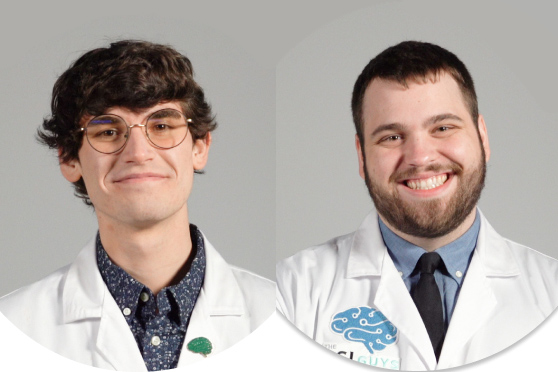
\includegraphics[width=\linewidth,height=39mm,keepaspectratio]{assets/history/bci-guys-rit.jpg}
      \par\smallskip{\scriptsize Harrison Canning and Colin Fausnaught\newline Photo: RIT, 2021\par}
  \end{columns}
  {\tiny\color{NTXMuted}Sources: \href{https://www.bciguys.com/course}{The BCI Guys: course}; \href{https://www.rit.edu/news/rit-student-and-alumnus-follow-passion-neurotechnology}{RIT profile / photograph}\par}
  \note{[85:15--86:45] The BCI Guys offer another entry point: approachable science communication and demonstrations alongside a structured introductory course. Their own 2023 post credits The BCI Guys and NeuroTechX with creating Foundations of Neurotechnology. The course page also describes NeuroTechEDU materials; do not promise that every historical platform remains available. Harrison is pictured left and Colin right. These formats complement formal education and research training. My sponsorship of PBS Space Time and enthusiasm for Journey to the Microcosmos are personal statements, not NeuroTechX sponsorships or partnerships. The lesson is that people can discover the field through compelling content, then find peers and projects through the community.}
\end{frame}

\begin{frame}{MedARC and Sophont: open collaboration in deep learning}
  \begin{columns}[c,onlytextwidth]
    \column{.51\textwidth}
      \small
      \NTXPoint{Research beyond a single lab}{Open medical AI projects, journal clubs, and shared resources.}
      \NTXPoint{A concrete neurotech example}{MindEye and MindEye2: collaborative fMRI-to-image research with public code.}
      \NTXPoint{Community alongside a company}{Sophont connects researchers with MedARC's community and research resources.}
    \column{.44\textwidth}
      \centering
      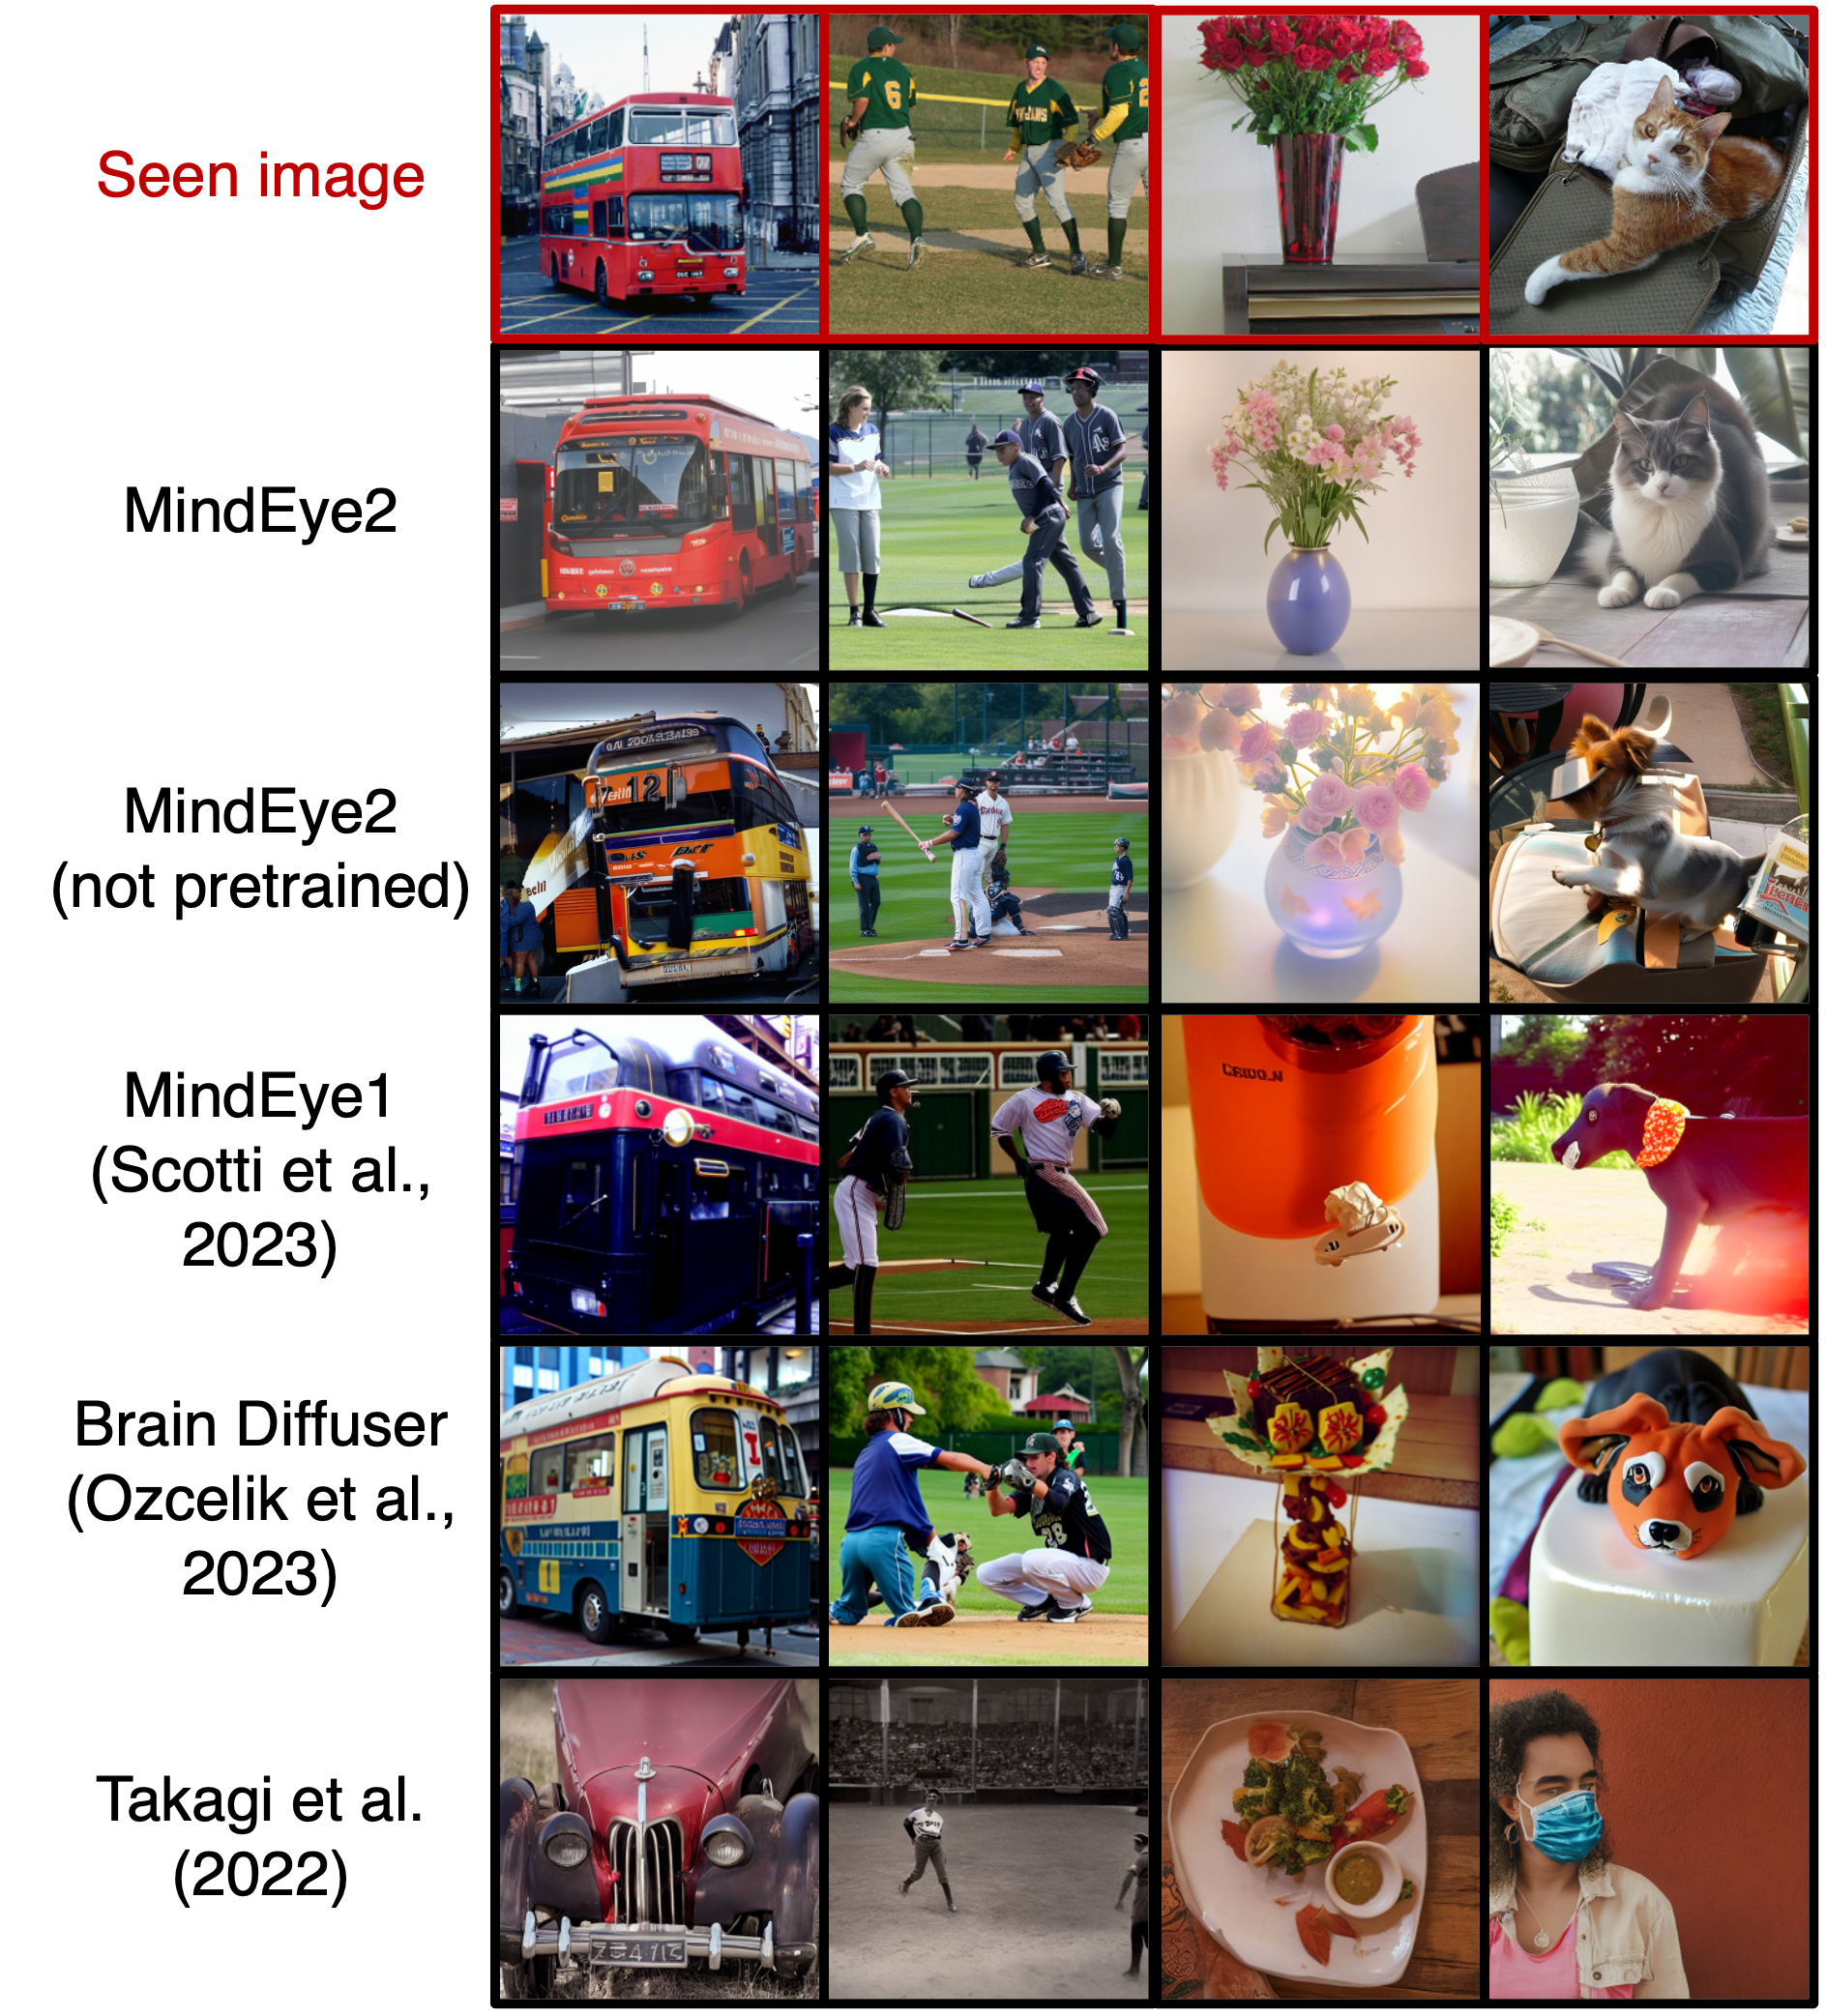
\includegraphics[width=\linewidth,height=46mm,keepaspectratio]{assets/history/medarc-mindeye2-results.png}
      \par\smallskip{\scriptsize MindEye2 --- published reconstruction examples\par}
  \end{columns}
  {\tiny\color{NTXMuted}Sources: \href{https://www.medarc.ai/}{MedARC}; \href{https://sophont.med/}{Sophont}; \href{https://medarc-ai.github.io/mindeye2/}{MindEye2}\par}
  \note{[86:45--88:45] The lesson is an organizational model for participating in deep-learning research: shared projects, expertise, resources, and public research artifacts. Sophont describes these community activities on its own site; access is not a guaranteed entitlement for every volunteer. MindEye2 concerns fMRI-to-image research under a particular experimental setup, not unrestricted mind reading or a consumer device. Do not imply all company assets or datasets are unrestricted. These are external examples, not NTX programs. Ask what our chapters can learn from this way of organizing research.}
\end{frame}

\begin{frame}{Agentic coding: Better Code, Better Science}
  \begin{columns}[c,onlytextwidth]
    \column{.46\textwidth}
      \NTXPoint{Russell A. Poldrack}{An open textbook on reproducible scientific software in the age of AI.}
      \NTXPoint{Beyond generating code}{Testing, workflows, and scientific validation.}
      \NTXPoint{For our community}{Shared reading and code review alongside hands-on projects.}
    \column{.49\textwidth}
      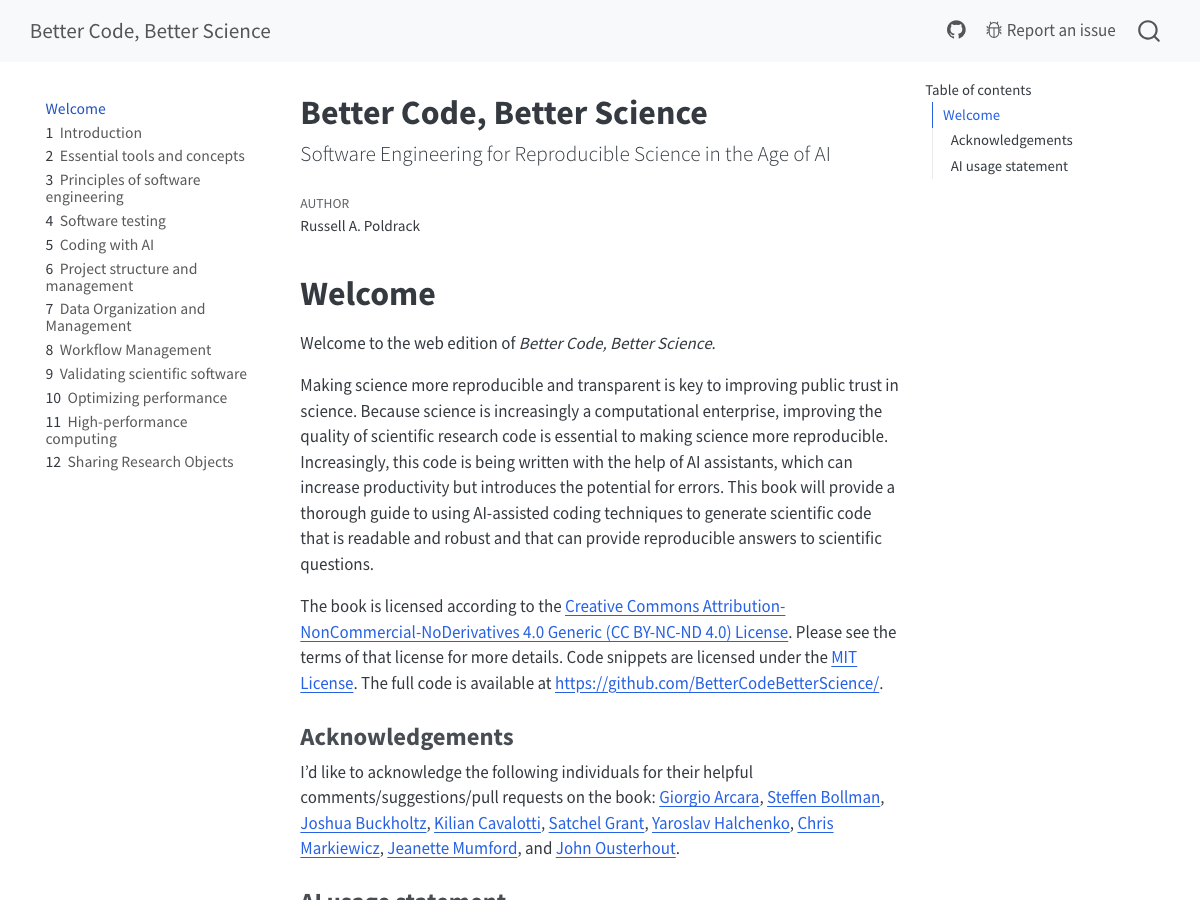
\includegraphics[width=\linewidth,height=48mm,keepaspectratio]{assets/history/better-code-better-science.png}
      \par\smallskip{\scriptsize Official web edition --- title-page screenshot\par}
  \end{columns}
  \NTXSource{https://bettercode-book.org/}{Russell A. Poldrack: Better Code, Better Science; text CC BY-NC-ND 4.0}
  \note{[88:45--89:45] Poldrack introduced this living textbook in May 2025. Its current web edition explicitly addresses readable, robust, reproducible scientific code in the age of AI. Chapters cover software engineering, testing, AI-assisted coding, workflows, and scientific validation. The image is a genuine screenshot of the official web title page, not a fabricated printed-book cover; no official cover was found in the current repository assets. Narrative text is licensed CC BY-NC-ND 4.0 and code snippets MIT. The proposal for NTX reading groups and code review is our suggested use, not a partnership or a course already launched.}
\end{frame}

\begin{frame}{Agentic research: learning the whole workflow}
  \begin{columns}[c,onlytextwidth]
    \column{.52\textwidth}
      \NTXPoint{Seyed Yahya Shirazi, Ph.D.}{Swartz Center for Computational Neuroscience, UC San Diego.}
      \NTXPoint{Agentic Research Course}{A ten-week course hosted by the Open Science Collective; open materials, CC BY 4.0.}
      \NTXPoint{From Git to research practice}{Coding agents, code quality, literature, manuscripts, figures, and neuroinformatics.}
    \column{.43\textwidth}
      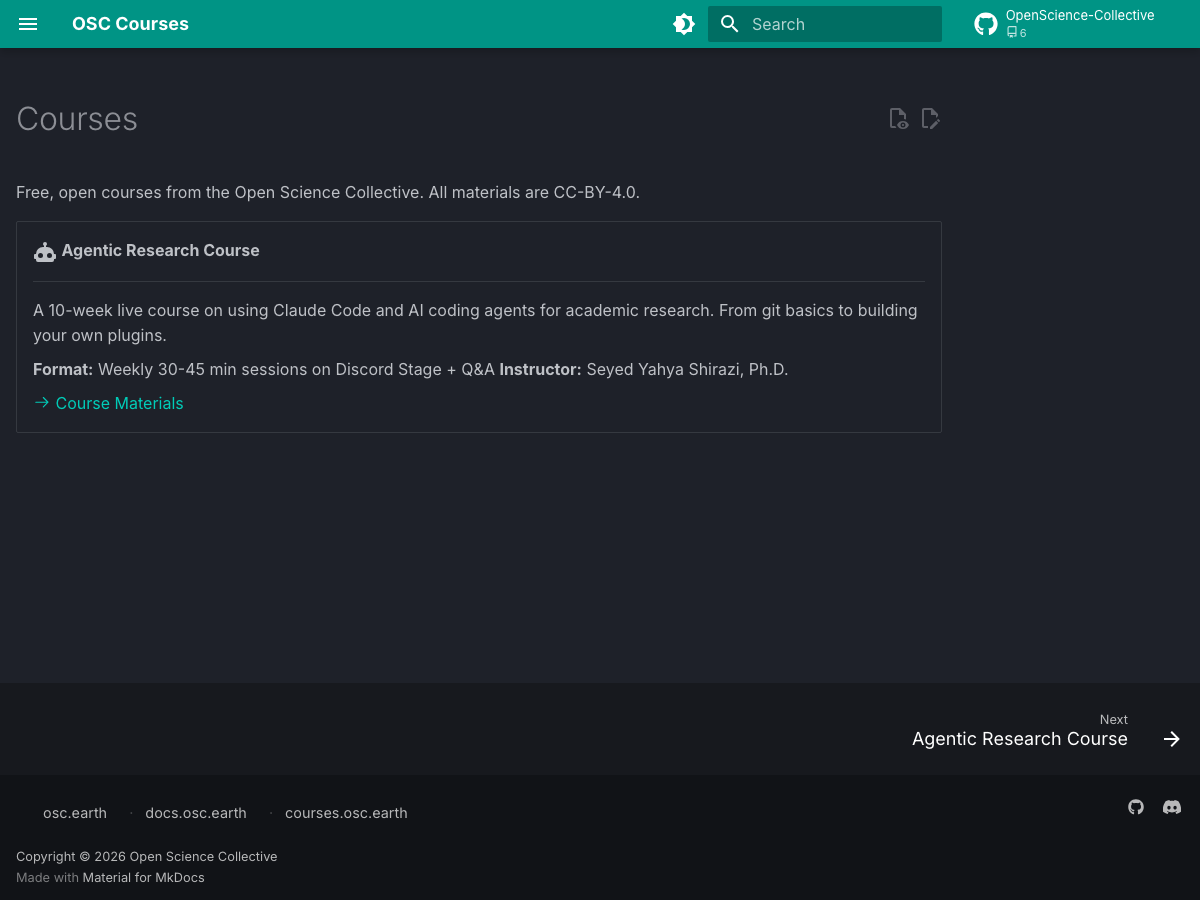
\includegraphics[width=\linewidth,height=44mm,keepaspectratio]{assets/history/agentic-research-course.png}
      \par\smallskip{\scriptsize Official Open Science Collective course page\par}
  \end{columns}
  {\tiny\color{NTXMuted}Sources: \href{https://courses.osc.earth/}{course site / screenshot}; \href{https://github.com/OpenScience-Collective/agentic-research-course}{syllabus, April--June 2026}; \href{https://neuromechanist.github.io/}{instructor}\par}
  \note{[89:45--90:45] This is the course Morgan referred to: Agentic Research Course, taught by Seyed Yahya Shirazi, a researcher at UCSD's Swartz Center for Computational Neuroscience. It is hosted by the Open Science Collective, not presented as a UCSD degree-credit offering. The repository schedules ten sessions from April 8 through June 9, 2026, covering Git, Claude Code, project management, CI/CD, literature search, grants, manuscripts, figures, neuroinformatics, and plugins. The syllabus lists BIDS, PsychoPy, and LSL in its neuroinformatics session. Course materials are free and CC BY 4.0; this does not mean commercial model usage is free. The repository limits its no-prior-coding prerequisite statement to weeks one and two. Do not promise recordings for every session or describe the spring schedule as upcoming. The link is a resource chapters could learn from, not a formal NTX partnership.}
\end{frame}

\NTXDivider{Take Away}


\begin{frame}{What would make these ambitions possible?}
  \begin{columns}[c,onlytextwidth]
    \column{.50\textwidth}
      \small
  \NTXPoint{Access to facilities and mentors}{Help students work beyond the equipment available in a typical club.}
  \NTXPoint{Projects that survive a competition}{Documentation, reproducible tests, and a handover to the next cohort.}
  \NTXPoint{A route to the next experiment}{Keep promising teams connected to collaborators and research opportunities.}
    \column{.46\textwidth}
      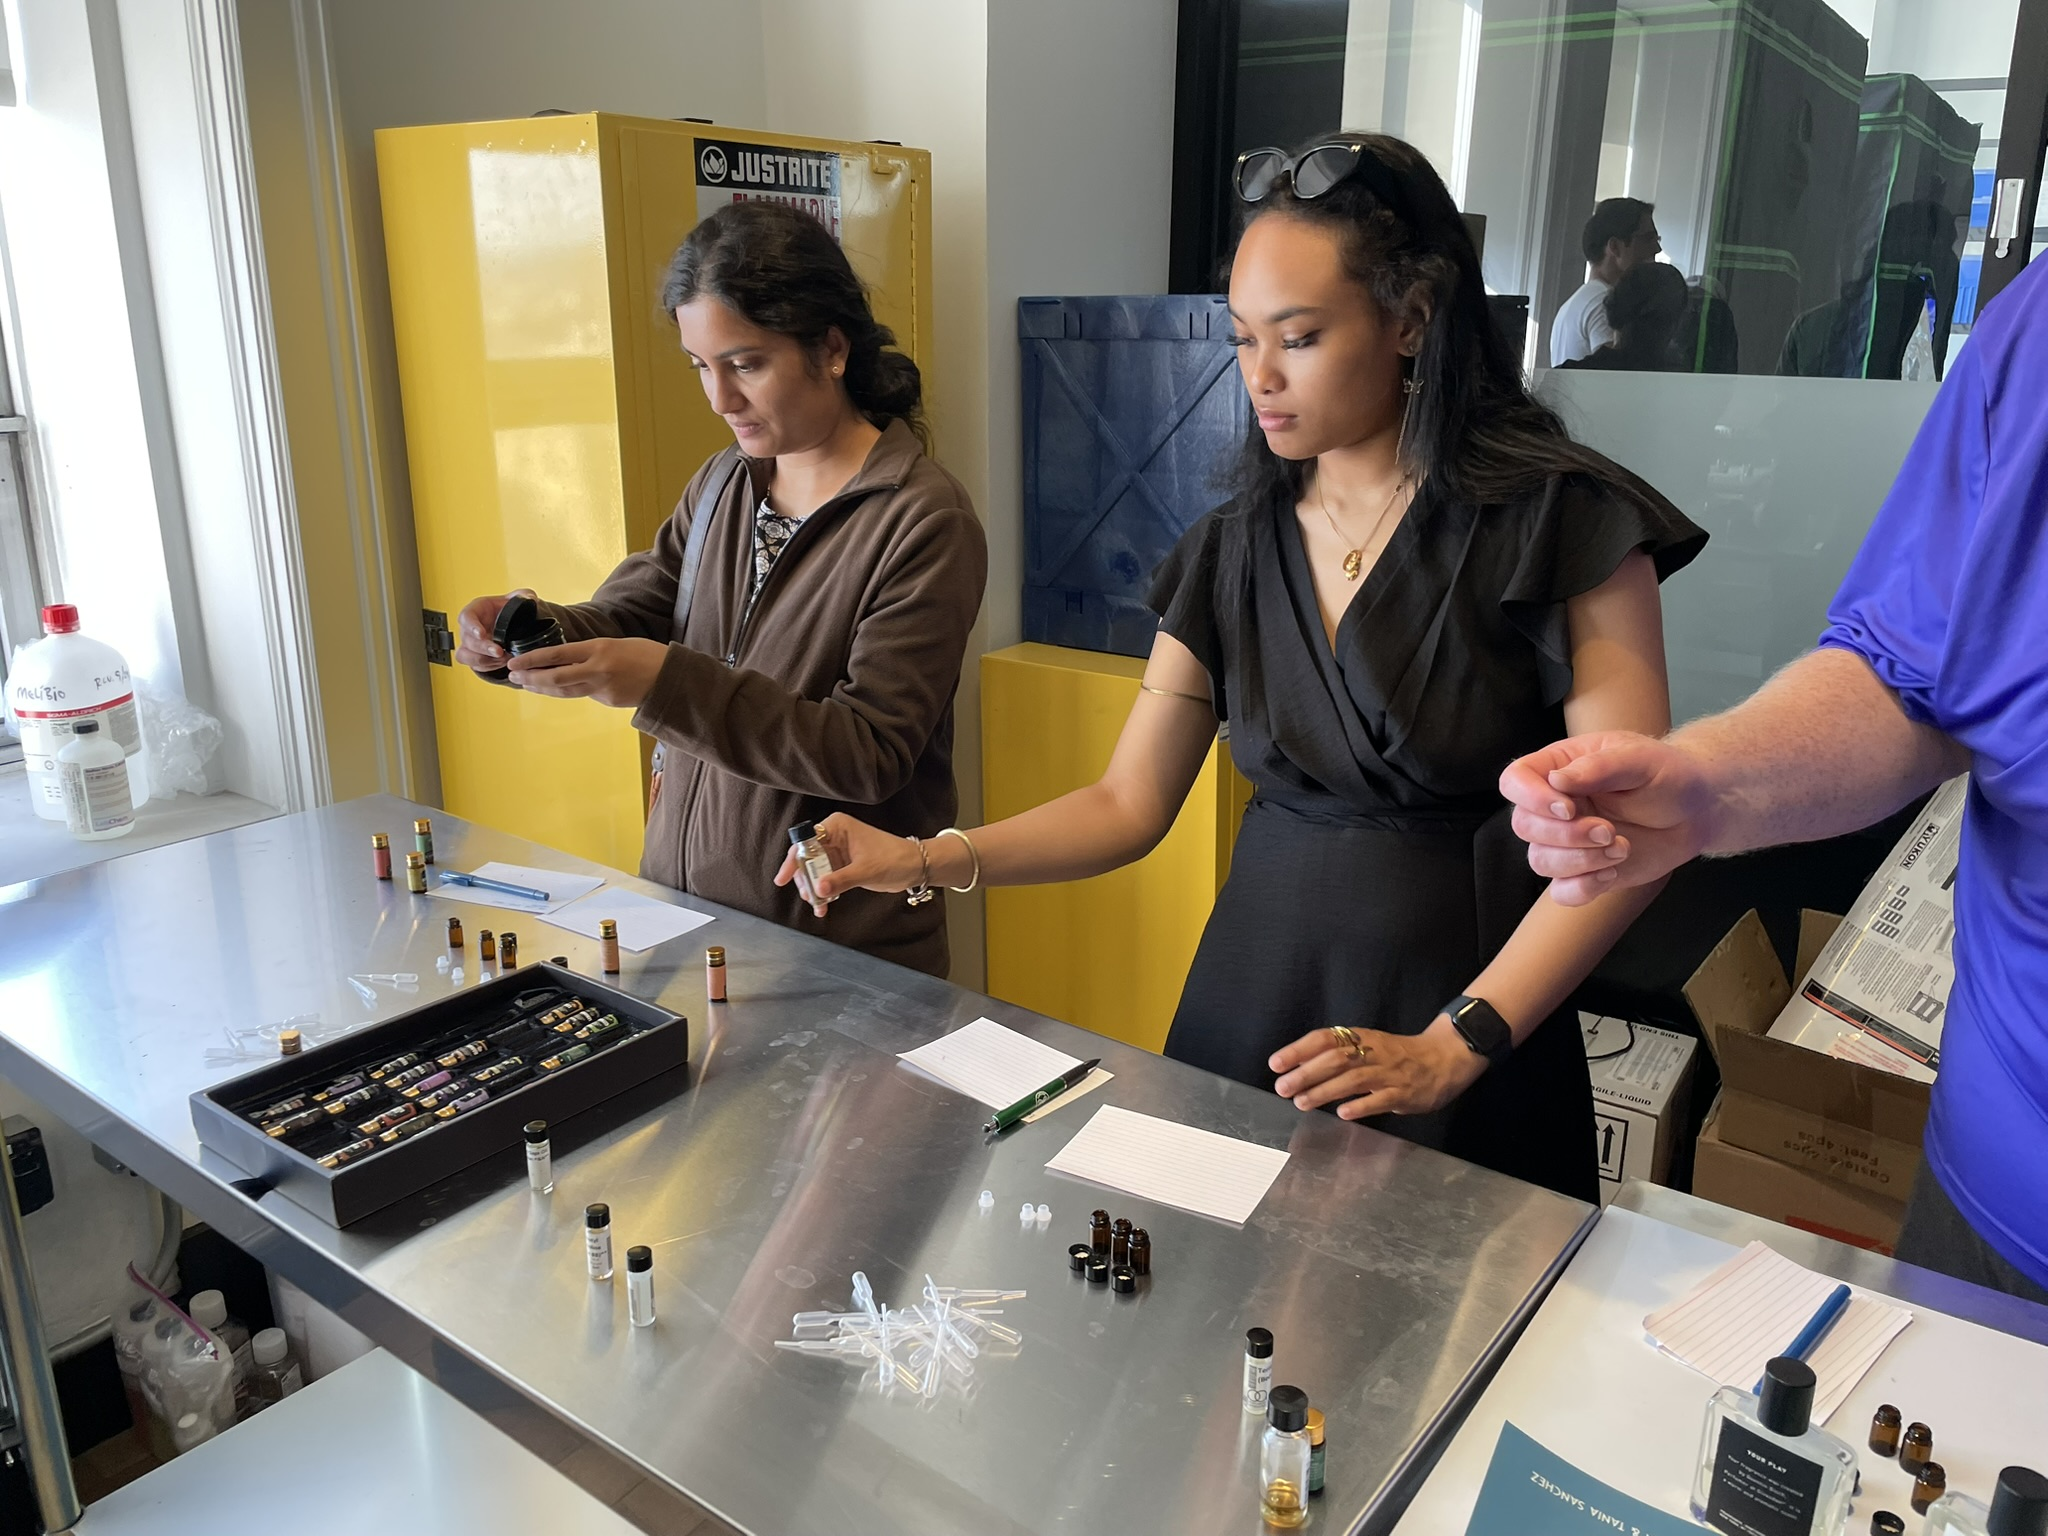
\includegraphics[width=\linewidth,height=44mm,keepaspectratio]{assets/history/biopunk-workshop.jpeg}\par\smallskip
      {\scriptsize Facilities and people to learn with\newline Photo: \href{https://biopunklab.com/}{Biopunk Lab}\par}
  \end{columns}
  \note{[90:45--91:45] These are proposed priorities, not new NTX commitments or claims that access is already secured. Connect the examples: quantum sensing needs characterization; MRI needs systems integration; fabrication needs facilities; sustained research needs teams that continue. Open curricula, collaborative research, and evaluated coding agents add new ways to participate. Invite the audience to contribute expertise and access.}
\end{frame}

\begin{frame}{A founder can also be a community contributor}
  \begin{columns}[c,onlytextwidth]
    \column{.50\textwidth}
      \small
  \NTXPoint{Bring a question people can work on}{A technical problem, an experiment, or a result to examine together.}
  \NTXPoint{Share something useful}{Documentation, a reproducible example, a workshop, or time helping another builder.}
  \NTXPoint{Build relationships through the work}{Meet people by learning, making, and contributing alongside them.}
    \column{.46\textwidth}
      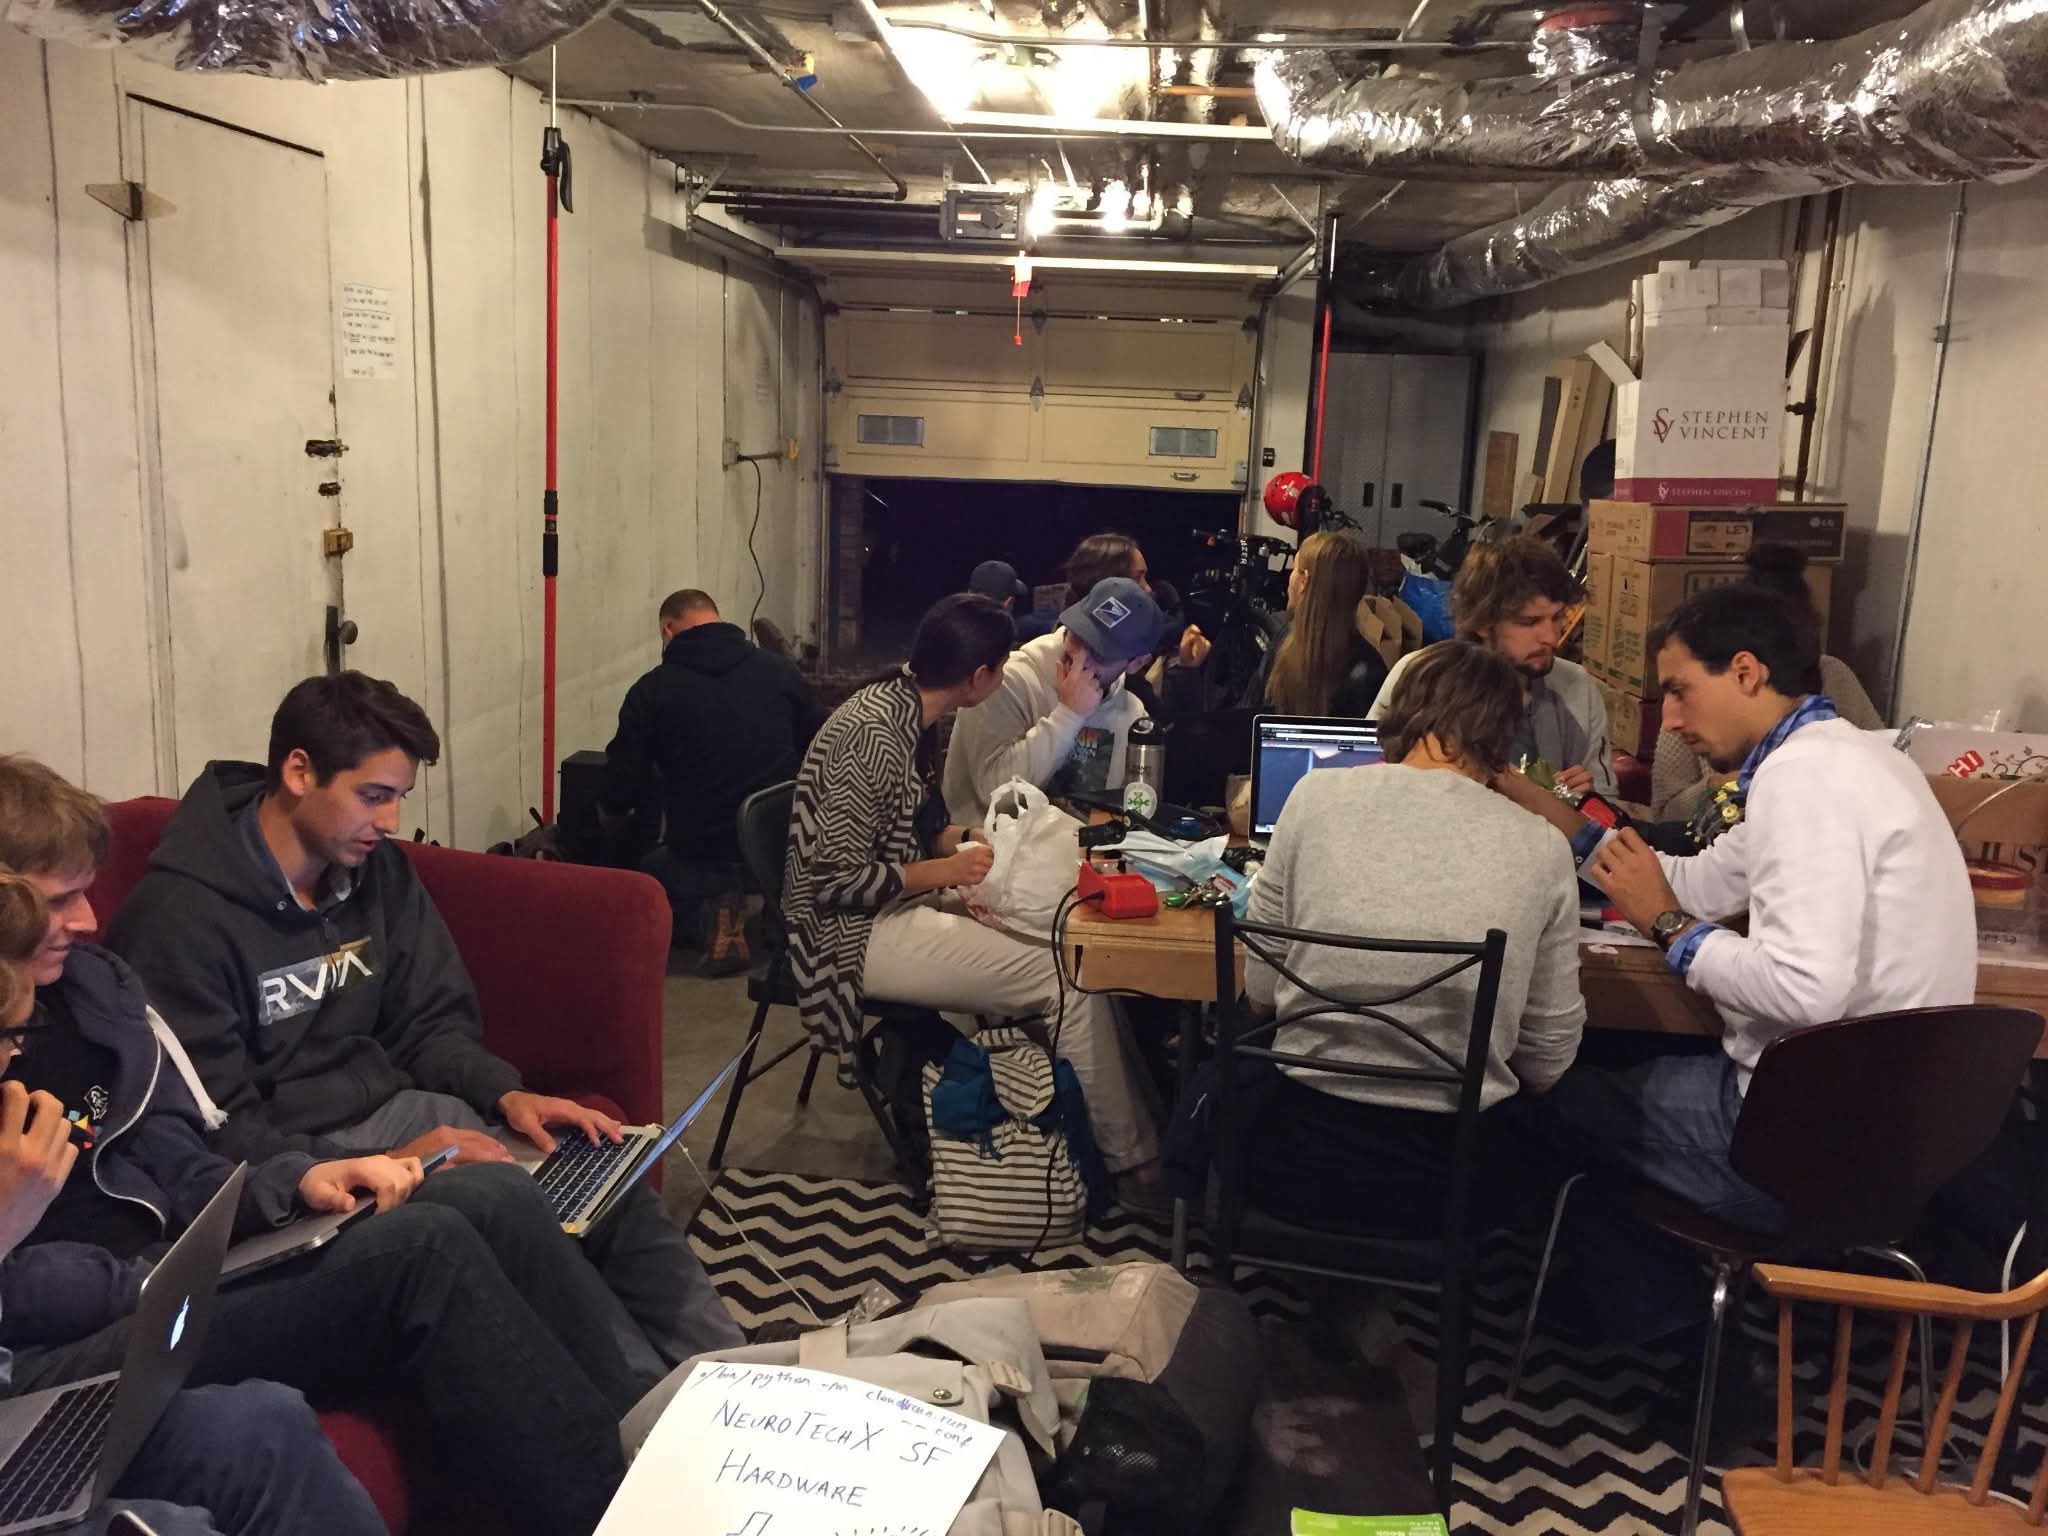
\includegraphics[width=\linewidth,height=44mm,keepaspectratio]{assets/chapters/san-francisco-original-hacknight.jpg}\par\smallskip
      {\scriptsize Start by working on something together\newline Original SF Hacknights --- Morgan's photo\par}
  \end{columns}
  \note{[91:45--93:45] This is an invitation to participate, grounded in the existing formats. It does not promise cofounder matching, funding, regulatory support, or access to a particular partner. Invite founders to think about what they can add to the community as well as what they hope to find. This is discussion framing, not an organizational commitment.}
\end{frame}


\begin{frame}{What can we build and learn together?}
  \begin{columns}[T,onlytextwidth]
    \column{.48\textwidth}
      \centering
      \textbf{Join NTX}\par\smallskip
      {\setlength{\fboxsep}{3mm}\colorbox{white}{\color{black}\qrcode[height=31mm,level=M,hyperlink=false]{https://bit.ly/ntx-slack}}}\par\smallskip
      {\small\href{https://bit.ly/ntx-slack}{bit.ly/ntx-slack}\par}
      {\scriptsize NeuroTechX Slack community\par}
    \column{.48\textwidth}
      \centering
      \textbf{Slides \& LaTeX repo}\par\smallskip
      {\setlength{\fboxsep}{3mm}\colorbox{white}{\color{black}\qrcode[height=31mm,level=M,hyperlink=false]{https://github.com/m9h/neurotechx-presentations}}}\par\smallskip
      {\scriptsize\href{https://github.com/m9h/neurotechx-presentations}{github.com/m9h/neurotechx-presentations}\par}
      {\scriptsize\color{NTXMuted}Public repository --- slides and LaTeX source\par}
  \end{columns}
  \medskip
  {\small Morgan Hough \quad \href{mailto:mhough@neurotechx.com}{mhough@neurotechx.com}\par}
  \note{[93:45--94:45] Thank the audience. Invite participation in the next generation of student projects. This expanded working version is approximately 67 minutes including acknowledgements, before discussion. Confirm the event slot before delivery.}
  \note{The QR codes encode https://bit.ly/ntx-slack and https://github.com/m9h/neurotechx-presentations. The latter comes from this repository's origin remote. Morgan authorized public release on September 6, 2026. The repository is public; the QR code opens its slides, PDFs and LaTeX source.}
\end{frame}

\section{Acknowledgements}
\begin{frame}{Acknowledgements}
  \begin{columns}[T,onlytextwidth]
    \column{.47\textwidth}
      \textbf{Board Members}\par\smallskip
      \begin{minipage}[t]{.48\linewidth}
        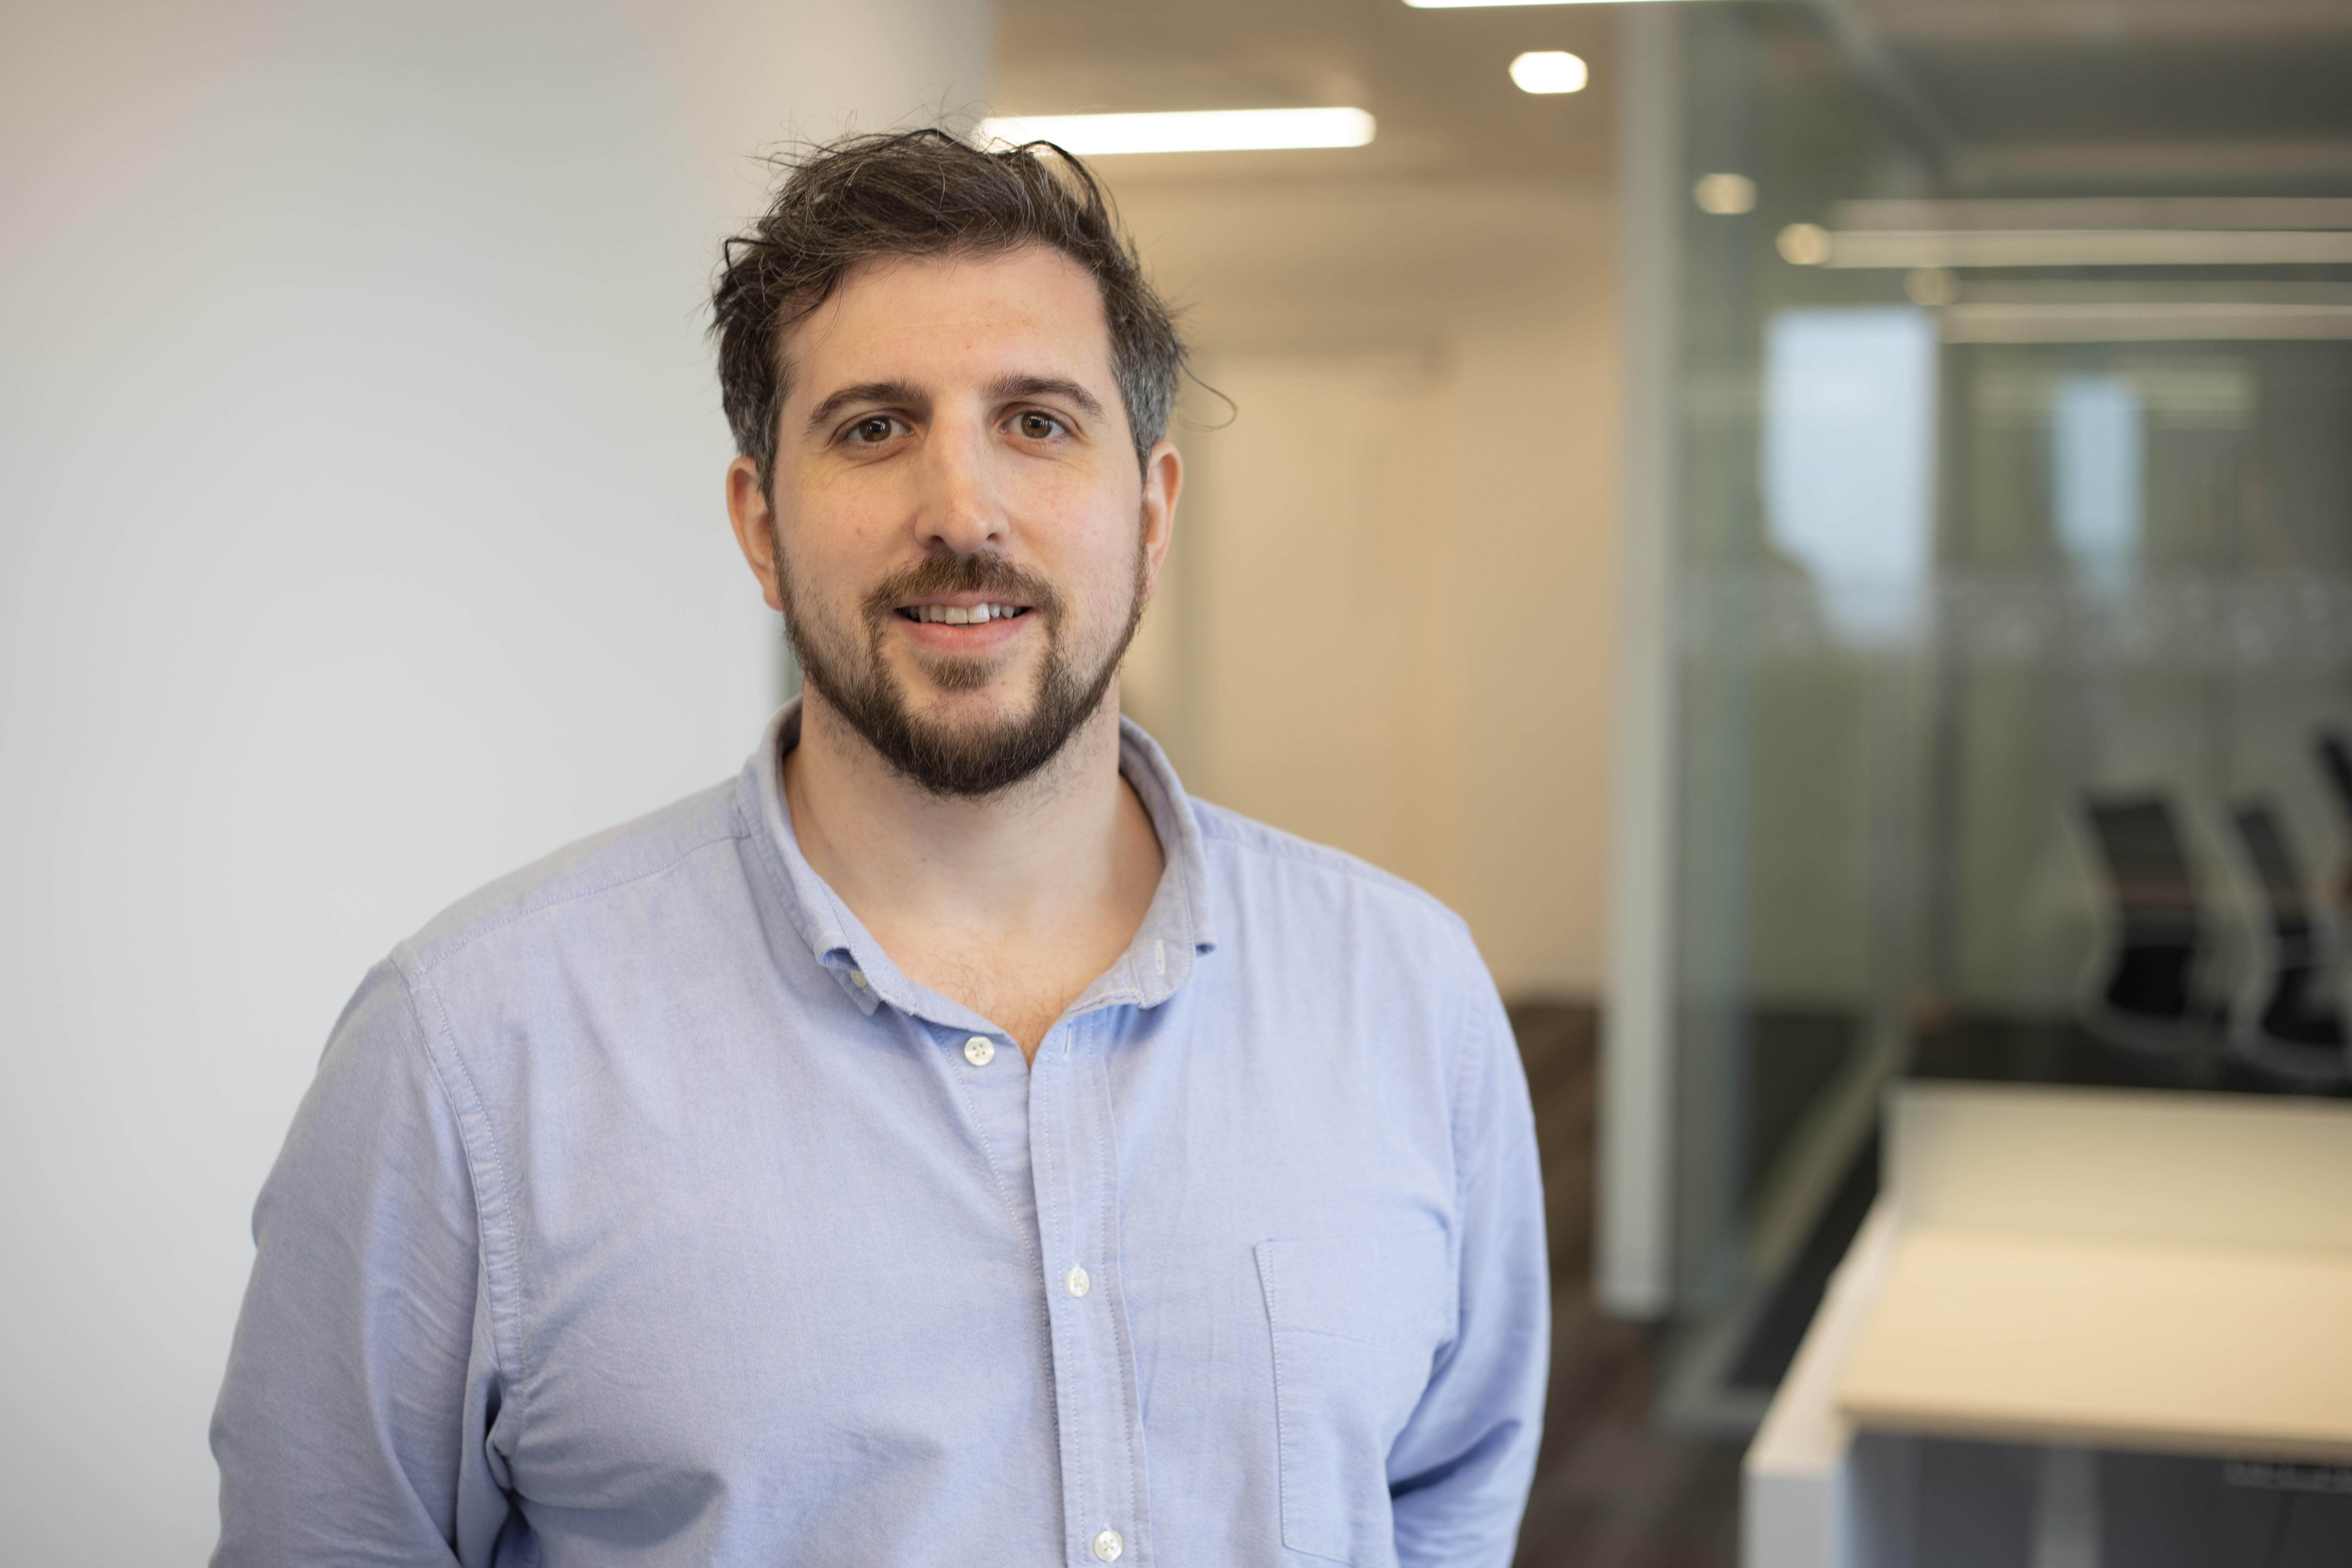
\includegraphics[width=\linewidth,height=21mm,keepaspectratio]{assets/people/john-griffiths.jpg}
        \par\smallskip{\small John Griffiths\par}
      \end{minipage}\hfill
      \begin{minipage}[t]{.48\linewidth}
        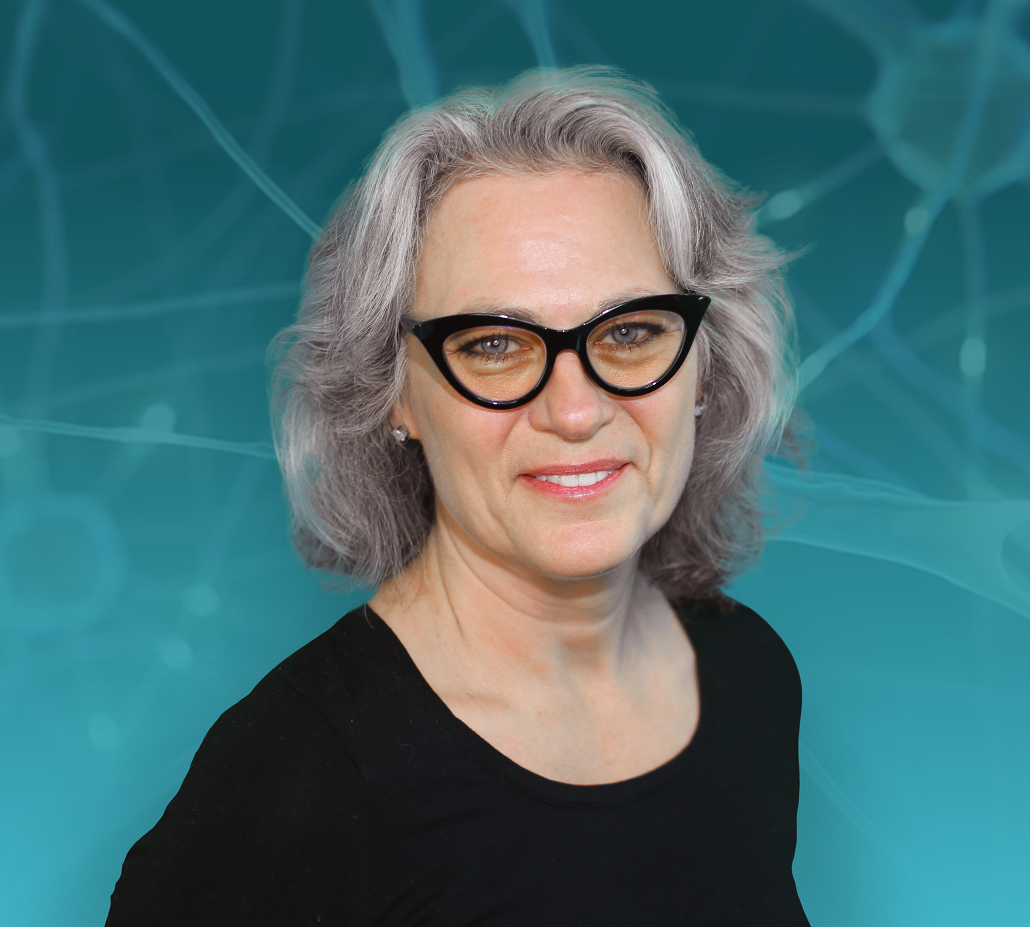
\includegraphics[width=\linewidth,height=21mm,keepaspectratio]{assets/people/susan-boehnke.png}
        \par\smallskip{\small Susan Boehnke\par}
      \end{minipage}
      \par\medskip
      {\small
        \textbf{BCIWiki} --- Landon Burress\par\medskip
        \textbf{MOABB} --- Bruno Aristimunha\par
        Lead developer\par\medskip
        \textbf{NeuroTechX SLC} --- Leonardo Ferrisi\par
      }
    \column{.48\textwidth}
      \small
      \setlength{\medskipamount}{3pt}
      \NTXPoint{Officers}{Han Nyguen and Dhruv Mehrotra}
      \NTXPoint{NTX Content Laboratory}{Sophie Valentine}
      \NTXPoint{CogLab / Learning Planet Institute}{Romain Rouyer and Hans Rajoharison}
      \NTXPoint{NeuroTechX Berlin}{Cris Michelli and Mitch Altman}
      \NTXPoint{Greater Bay Area}{Kimberley Cheung\newline Hong Kong / Shenzhen / Guangzhou}
  \end{columns}
  \medskip
  {\tiny\color{NTXMuted}Portraits: \href{https://www.camh.ca/en/science-and-research/science-and-research-staff-directory/john-griffths}{CAMH}; \href{https://neurotechmicrocreds.com/our-team/susan-boehnke-phd/}{Queen's NeuroTech Microcredential Program}\par}
  \note{[94:45--95:15] Thank these colleagues for their contributions. Morgan supplied Dhruv Mehrotra's correction and Kimberley Cheung's acknowledgement for Hong Kong, Shenzhen, and Guangzhou. CogLab's official team page verifies Romain Rouyer and Hans Rajoharison. Greater Bay Area is shorthand for Guangdong--Hong Kong--Macao Greater Bay Area, which includes these three cities and others; it does not imply Kimberley has a formal role across the entire region. Sources: https://coglab.fr/about/team/ and https://www.bayarea.gov.hk/en/about/overview.html.}
  \note{Morgan requested acknowledgement of Landon with BCIWiki and Bruno as MOABB lead developer. Landon's own BCIWiki contribution to Open Neuroscience spells his name Landon Burress: https://open-neuroscience.com/en/post/bciwiki/. Bruno's own GitHub profile verifies Bruno Aristimunha and his MOABB involvement: https://github.com/bruAristimunha. The lead-developer role is supplied by Morgan.}
\end{frame}
